\documentclass{article}

  % packages
    % basic stuff for rendering math
    \usepackage[letterpaper, top=1in, bottom=1in, left=1in, right=1in]{geometry}
    \usepackage[utf8]{inputenc}
    \usepackage[english]{babel}
    \usepackage{amsmath} 
    \usepackage{amssymb}
    \usepackage{polynom}
    \usepackage{longdivision}

    % extra math symbols and utilities
    \usepackage{mathtools}        % for extra stuff like \coloneqq
    \usepackage{mathrsfs}         % for extra stuff like \mathsrc{}
    \usepackage{centernot}        % for the centernot arrow 
    \usepackage{bm}               % for better boldsymbol/mathbf 
    \usepackage{enumitem}         % better control over enumerate, itemize
    \usepackage{hyperref}         % for hypertext linking
    \usepackage{xr-hyper}
    \usepackage{fancyvrb}          % for better verbatim environments
    \usepackage{newverbs}         % for texttt{}
    \usepackage{xcolor}           % for colored text 
    \usepackage{listings}         % to include code
    \usepackage{lstautogobble}    % helper package for code
    \usepackage{parcolumns}       % for side by side columns for two column code
    

    % page layout
    \usepackage{fancyhdr}         % for headers and footers 
    \usepackage{lastpage}         % to include last page number in footer 
    \usepackage{parskip}          % for no indentation and space between paragraphs    
    \usepackage[T1]{fontenc}      % to include \textbackslash
    \usepackage{footnote}
    \usepackage{etoolbox}

    % for custom environments
    \usepackage{tcolorbox}        % for better colored boxes in custom environments
    \tcbuselibrary{breakable}     % to allow tcolorboxes to break across pages

    % figures
    \usepackage{pgfplots}
    \pgfplotsset{compat=1.18}
    \usepackage{float}            % for [H] figure placement
    \usepackage{tikz}
    \usepackage{tikz-cd}
    \usepackage{circuitikz}
    \usetikzlibrary{arrows}
    \usetikzlibrary{positioning}
    \usetikzlibrary{calc}
    \usepackage{graphicx}
    \usepackage{caption} 
    \usepackage{subcaption}
    \captionsetup{font=small}

    % for tabular stuff 
    \usepackage{dcolumn}

    \usepackage[nottoc]{tocbibind}
    \pdfsuppresswarningpagegroup=1
    \hfuzz=5.002pt                % ignore overfull hbox badness warnings below this limit

  % New and replaced operators
    \let\lbrack\relax
    \let\rbrack\relax
    \let\Char\relax
    \let\O\relax
    \newcommand{\lbrack}{[}
    \newcommand{\rbrack}{]}
    \DeclareMathOperator{\Char}{char}
    \DeclareMathOperator{\Tr}{Tr}
    \DeclareMathOperator{\Tran}{Tran}
    \DeclareMathOperator{\Sym}{Sym}
    \DeclareMathOperator{\Span}{span}
    \DeclareMathOperator{\Aut}{Aut}
    \DeclareMathOperator{\End}{End}
    \DeclareMathOperator{\im}{Im}
    \DeclareMathOperator{\ev}{ev}
    \DeclareMathOperator{\Dih}{Dih}
    \DeclareMathOperator{\O}{O}
    \DeclareMathOperator{\sign}{sgn}
    \DeclareMathOperator{\SO}{SO}
    \DeclareMathOperator{\Div}{div}
    \DeclareMathOperator{\ord}{ord}
    \DeclareMathOperator{\curl}{curl}
    \DeclareMathOperator{\Isom}{Isom}
    \DeclareMathOperator{\GL}{GL}
    \DeclareMathOperator{\SU}{SU}
    \DeclareMathOperator{\SL}{SL}
    \DeclareMathOperator{\GA}{GA}
    \DeclareMathOperator{\std}{std}
    \DeclareMathOperator{\Cov}{Cov}
    \DeclareMathOperator{\Var}{Var}
    \DeclareMathOperator{\Corr}{Corr}
    \DeclareMathOperator{\Int}{Int}
    \DeclareMathOperator{\Id}{Id}
    \DeclareMathOperator{\Lie}{Lie}
    \DeclareMathOperator{\Hom}{Hom}
    \DeclareMathOperator{\Alt}{Alt}
    \DeclareMathOperator{\rank}{rank}
    \DeclareMathOperator{\conv}{conv}
    \DeclareMathOperator{\aff}{aff}
    \DeclareMathOperator{\arccot}{arccot}
    \DeclareMathOperator*{\argmin}{\arg\!\min}
    \DeclareMathOperator*{\argmax}{\arg\!\max}
    \newcommand{\qed}{\hfill$\blacksquare$}     % I like QED squares to be black

  % Custom Environments
    \newtcolorbox[auto counter, number within=section]{question}[1][]
    {
      colframe = orange!25,
      colback  = orange!10,
      coltitle = orange!20!black,  
      breakable, 
      title = \textbf{Question \thetcbcounter ~(#1)}
    }

    \newtcolorbox[auto counter, number within=section]{exercise}[1][]
    {
      colframe = teal!25,
      colback  = teal!10,
      coltitle = teal!20!black,  
      breakable, 
      title = \textbf{Exercise \thetcbcounter ~(#1)}
    }
    \newtcolorbox[auto counter, number within=section]{solution}[1][]
    {
      colframe = violet!25,
      colback  = violet!10,
      coltitle = violet!20!black,  
      breakable, 
      title = \textbf{Solution \thetcbcounter}
    }
    \newtcolorbox[auto counter, number within=section]{lemma}[1][]
    {
      colframe = red!25,
      colback  = red!10,
      coltitle = red!20!black,  
      breakable, 
      title = \textbf{Lemma \thetcbcounter ~(#1)}
    }
    \newtcolorbox[auto counter, number within=section]{theorem}[1][]
    {
      colframe = red!25,
      colback  = red!10,
      coltitle = red!20!black,  
      breakable, 
      title = \textbf{Theorem \thetcbcounter ~(#1)}
    } 
    \newtcolorbox[auto counter, number within=section]{proposition}[1][]
    {
      colframe = red!25,
      colback  = red!10,
      coltitle = red!20!black,  
      breakable, 
      title = \textbf{Proposition \thetcbcounter ~(#1)}
    } 
    \newtcolorbox[auto counter, number within=section]{corollary}[1][]
    {
      colframe = red!25,
      colback  = red!10,
      coltitle = red!20!black,  
      breakable, 
      title = \textbf{Corollary \thetcbcounter ~(#1)}
    } 
    \newtcolorbox[auto counter, number within=section]{proof}[1][]
    {
      colframe = orange!25,
      colback  = orange!10,
      coltitle = orange!20!black,  
      breakable, 
      title = \textbf{Proof. }
    } 
    \newtcolorbox[auto counter, number within=section]{definition}[1][]
    {
      colframe = yellow!25,
      colback  = yellow!10,
      coltitle = yellow!20!black,  
      breakable, 
      title = \textbf{Definition \thetcbcounter ~(#1)}
    } 
    \newtcolorbox[auto counter, number within=section]{example}[1][]
    {
      colframe = blue!25,
      colback  = blue!10,
      coltitle = blue!20!black,  
      breakable, 
      title = \textbf{Example \thetcbcounter ~(#1)}
    } 
    \newtcolorbox[auto counter, number within=section]{code}[1][]
    {
      colframe = green!25,
      colback  = green!10,
      coltitle = green!20!black,  
      breakable, 
      title = \textbf{Code \thetcbcounter ~(#1)}
    } 

    \definecolor{dkgreen}{rgb}{0,0.6,0}
    \definecolor{gray}{rgb}{0.5,0.5,0.5}
    \definecolor{mauve}{rgb}{0.58,0,0.82}
    \definecolor{lightgray}{gray}{0.93}

    % default options for listings (for code)
    \lstset{
      autogobble,
      frame=ltbr,
      language=C,                           % the language of the code
      aboveskip=3mm,
      belowskip=3mm,
      showstringspaces=false,
      columns=fullflexible,
      keepspaces=true,
      basicstyle={\small\ttfamily},
      numbers=left,
      firstnumber=1,                        % start line number at 1
      numberstyle=\tiny\color{gray},
      keywordstyle=\color{blue},
      commentstyle=\color{dkgreen},
      stringstyle=\color{mauve},
      backgroundcolor=\color{lightgray}, 
      breaklines=true,                      % break lines
      breakatwhitespace=true,
      tabsize=3, 
      xleftmargin=2em, 
      framexleftmargin=1.5em, 
      stepnumber=1
    }

  % Page style
    \pagestyle{fancy}
    \fancyhead[L]{Abstract Algebra}
    \fancyhead[C]{Muchang Bahng}
    \fancyhead[R]{August 2021} 
    \fancyfoot[C]{\thepage / \pageref{LastPage}}
    \renewcommand{\footrulewidth}{0.4pt}          % the footer line should be 0.4pt wide
    \renewcommand{\thispagestyle}[1]{}  % needed to include headers in title page

  % external documents 
    \externaldocument[st-]{../Set_Theory/paper}[../Set_Theory/paper.pdf] 
    \externaldocument[pst-]{../Point_Set_Topology/paper}[../Point_Set_Topology/paper.pdf] 

\begin{document}

\title{Abstract Algebra}
\author{Muchang Bahng}
\date{Spring 2024}

\maketitle
\tableofcontents
\pagebreak 

This covers computability theory, complexity theory, and automata theory. 
Alphabet. Boolean logic


\section{Group-Like Structures} 

\subsection{Semigroups and Monoids}

  Now the endowment of some structures gives rise to the following. Usually, we will start with the most general algebraic structures and then as we endow them with more structure, we can prove more properties. Let's talk about the most basic type of algebraic structure. If you have a set $S$ and some associative operation on it, we have a semigroup. 

  \begin{definition}[Semigroup]
    A \textbf{semigroup} $(S, \cdot)$ is a set $S$ with an associative binary operation 
    \begin{equation}
      \cdot : S \times S \to S
    \end{equation}
  \end{definition} 

  \begin{example}[Continuous Time Markov Chain]
    Let $(\Omega, \mathcal{F}, \mathbb{P})$ be a probability space and $(S, \mathcal{S})$ a measurable space. Then, a homogeneous continuous-time Markov chain is a stochastic process $\{X_t\}_{t \geq 0}$ taking values in $S$ (i.e. $X_t: \Omega \rightarrow S$) satisfying the \textbf{Markov property}: for every bounded measurable $f$ and and $t, s \geq 0$, 
    \begin{equation}
      \mathbb{E}[ f(X_{t + s}) \mid \{X_r\}_{r \leq t} ] = \mathbb{E}[ f(X_{t + s}) \mid X_t ] = (P_s f)(X_t)
    \end{equation}
    The set $\{P_t\}_{t \geq 0}$ with the composition operation gives us the \textit{Markov semigroup}. 
  \end{example} 

  To be honest the above example is the only time I have every seen a semigroup come up, so we proceed immediately to the next structure. 

  \begin{definition}[Monoid]
    A \textbf{monoid} $(M, \cdot, e)$ is a semigroup with an identity element $e \in M$ such that given a $m \in M$
    \begin{equation}
      e \cdot m = m \cdot e = m
    \end{equation}
  \end{definition} 

  We first should ask whether the identity is unique in a monoid. It turns out it is. 

  \begin{lemma}[Uniqueness of Monoid Identity]
    The identity $e$ of a monoid $M$ is unique. 
  \end{lemma}
  \begin{proof}
    Assume not, i.e. there are 2 identities $e \neq e^\prime$. But then 
    \begin{equation}
      e = e e^\prime = e^\prime \implies e = e^\prime
    \end{equation}
    where the implication follows from transitivity of equivalence relations. 
  \end{proof} 

  From set theory, we have directly worked with two examples of monoids. 

  \begin{example}[Set Operations]
    Let $S$ be any nonempty set. Then $(2^S, \cup, \emptyset)$ and $(2^S, \cap, S)$ are monoids. So it seems that there are flavors of algebra that aren't really separable from set theory. 
  \end{example}

  \begin{definition}[Submonoid]
    Given a monoid $(M, \ast)$, let $M^\prime \subset M$. If the restriction of $\ast$ to $M^\prime \times M^\prime$ is closed in $M^\prime$, then we can define the \textbf{submonoid} $(M^\prime, \ast)$. 
  \end{definition} 

  It may seem like the identity of a submonoid must be the identity of the monoid, but this is not always the case. We may take a subset $M^\prime \subset M$ such that $\cdot$ is closed in $M^\prime$ and there may be some $e^\prime \in M^\prime, e^\prime \neq e$ such that it acts like an identity on $M^\prime$. 

  \begin{example}[Identities of Submonoids May Not be the Same]
    Let $(M, \times, I)$ be the monoid of $2 \times 2$ matrices over $\mathbb{R}$ with the identity matrix $I$, and let $M^\prime$ be the set of matrices of form 
    \begin{equation}
      \begin{pmatrix} a & 0 \\ 0 & 0 \end{pmatrix} \text{ for } a \in \mathbb{R}, \qquad I^\prime = \begin{pmatrix} 1 & 0 \\ 0 & 0 \end{pmatrix}
    \end{equation}
    Then $(M^\prime, \times, I^\prime)$ is a submonoid with a different identity element. 
  \end{example}

  \begin{example}[$\mathbb{N}$ is a Monoid]
    The natural numbers, defined \hyperref[st-naturals]{here} are a monoid. More specifically, 
    \begin{enumerate}
      \item $(\mathbb{N}, +, 0)$ is a monoid under addition. 
      \item $(\mathbb{N}, \times, 1)$ is a monoid under multiplication. 
      \item $(2\mathbb{N}, +, 0)$ is a monoid under addition, where $2\mathbb{N}$ is the set of all even numbers. 
      \item $2\mathbb{N}$ cannot be a monoid since $1 \not\in 2\mathbb{N}$. 
    \end{enumerate}
  \end{example}

  \begin{definition}[Monoid of Transformations]
    Given a set $S$, consider the set of all functions $S^S \coloneqq \{f: S \rightarrow S\}$. Then, with function composition $\circ$, $(S^S, \circ)$ is a monoid with the identity function $e: x \mapsto x$ as the identity element. This is called the \textbf{monoid of transformations} of $S$. 
  \end{definition} 

  \begin{theorem}[Cardinality of Monoid of Transformations]
    If $|S| = n$, then the monoid of transformations has cardinality $n^n$. 
  \end{theorem}

\subsection{Groups} 

  Now we look at a specific case of monoids where invertibility is defined. The existence of inverses produces a whole suite of interesting properties, as we will see. 
  
  \begin{definition}[Group]
    A \textbf{group} $(G, \cdot)$ is a set with binary operation $x \cdot y$---also written as $xy$---having the following properties.
    \begin{enumerate}
      \item \textit{Closure}. $x, y \in G \implies xy \in G$\footnote{but not necessarily $xy  = yx$}
      \item \textit{Associativity}. $\forall x, y, z \in G, x(yz) = (xy)z$
      \item \textit{Identity}. $\exists e \in G$ s.t. $\forall x \in G, xe = ex = x$
      \item \textit{Inverses}. $\forall x \in G \; \exists x^{-1} \in G$ s.t. $x x^{-1} = x^{-1} x = e$
    \end{enumerate}
    The \textbf{order} of a group is the cardinality $|G|$. An \textbf{abelian group} $(A, +)$ is a group where $+$ is commutative.\footnote{Note that I switched the notation from $\ast$ to $+$. By convention and to avoid confusion, $+$ denotes commutative operations. }
  \end{definition} 

  This is an extremely simple structure, and the first thing we should prove is the uniqueness of the identity and inverses. 

  \begin{lemma}[Uniqueness of Identity and Inverse]
    The identity and the inverse is unique, and for any $a, b$, the equation $x*a = b$ has the unique solution $x = b* a^{-1}$.
  \end{lemma}
  \begin{proof}
     Assume that there are two identities of group $(G,*)$, denoted $e_{1}, e_{2}$, where $e_{1} \neq e_{2}$. According to the properties of identities, $e_{1} = e_{1} * e_{2} = e_{2} \implies e_{1} = e_{2}$. \\
    As for uniqueness of a inverses, let $a$ be an element of $G$, with its inverses $a_{1}^{-1}, a_{2}^{-1}$. Then, 
    \begin{align*}
      a * a_{1}^{-1} = e & \implies a_{2}^{-1} * \Big(a * a_{1}^{-1} \Big)= a_{2}^{-1} * e \\
       & \implies \Big(a_{2}^{-1} * a \Big) * a_{1}^{-1} = a_{2}^{-1} \\
       & \implies e * a_{1}^{-1} = a_{2}^{-1}
    \end{align*}
    Since the inverse is unique, we can operate on each side of the equation $x*a = b$ to get $x*a*a^{-1} = b*a^{1} \implies x * e = x = b*a^{-1}$. Clearly, the derivation of this solution is unique since the elements that we have operated on are unique.
  \end{proof} 
  
  At this point, we can see that for each group there is a corresponding ``multiplication table'' defined by the operation. For example, we can create a set of $6$ elements $\{r_0, r_1, r_2, s_0, s_1, s_2\}$ and define the operation $\times$ as the following. 

  \begin{figure}[H]
    \centering 
    \begin{tabular}{c|cccccc}
      $\times$ & $r_0$ & $r_1$ & $r_2$ & $s_0$ & $s_1$ & $s_2$ \\
      \hline
      $r_0$ & $r_0$ & $r_1$ & $r_2$ & $s_0$ & $s_1$ & $s_2$ \\
      $r_1$ & $r_1$ & $r_2$ & $r_0$ & $s_1$ & $s_2$ & $s_0$ \\
      $r_2$ & $r_2$ & $r_0$ & $r_1$ & $s_2$ & $s_0$ & $s_1$ \\
      $s_0$ & $s_0$ & $s_2$ & $s_1$ & $r_0$ & $r_2$ & $r_1$ \\
      $s_1$ & $s_1$ & $s_0$ & $s_2$ & $r_1$ & $r_0$ & $r_2$ \\
      $s_2$ & $s_2$ & $s_1$ & $s_0$ & $r_2$ & $r_1$ & $r_0$ \\
    \end{tabular}
    \caption{Multiplication table for some group. Note that we can only write such a table explicitly for a group of finite elements. But even for arbitrary groups, we should think of the operation completely defining a possibly ``infinite'' table.} 
  \end{figure} 

  It is clear that in an abelian group, the multiplication table must be symmetric across the diagonal. 

  \begin{example}[Familiar Groups]
    So what are some examples of groups? 
    \begin{enumerate}
      \item $(\mathbb{N}, +)$ is not a group since $3 \in \mathbb{N}$ but $-3 \not\in \mathbb{N}$. It is a commutative monoid. 
      \item $(\mathbb{N}, \times)$ is not a group but is a commutative monoid. 
      \item $(\mathbb{Z}, +)$ is an abelian group. 
      \item $(\mathbb{Z}, \times)$ is not a group. 
      \item $(\mathbb{Q}, +)$ and $(\mathbb{Q} \setminus \{0\}, \times)$ are both abelian groups. 
      \item $(\mathbb{R}, +)$ and $(\mathbb{R} \setminus \{0\}, \times)$ are both abelian groups. 
      \item The set of all invertible $n \times n$ matrices with matrix multiplication, denoted $(\GL (\mathbb{R}^n), \times)$ is a non-abelian group. 
      \item The set of all functions on a given interval $[a,b]$ is abelian with respect to addition, defined as $(f+g)(x) \equiv f(x) + g(x)$. 
    \end{enumerate}
  \end{example}

  \begin{example}[Group of Invertible Elements of a Monoid]
    Given $x \in (M, \cdot, e)$, let $x$ be \textbf{invertible} if there exists $x^{-1} \in M$ s.t. $x x^{-1} = x^{-1} x = e$. Then, the submonoid $M^\prime$ of invertible elements of $M$ is a group. This must be proved. 
    \begin{enumerate}
      \item \textit{Closure}. If $x, y \in M^\prime$, then $x^{-1}, y^{-1} \in M^\prime$ since $(x^{-1})^{-1} = x$. Therefore $y^{-1} x^{-1} = (xy)^{-1} \in M^\prime$, and so $xy \in M^\prime$. 
      \item \textit{Identity}. $e^{-1} = e$ so $e \in M^\prime$. 
      \item \textit{Inverses}. Exists by definition. 
      \item \textit{Associativity}. Is inherited from associativity of $\cdot$ in $M$. 
    \end{enumerate}
  \end{example}

  Let's prove a little more about groups so that we have more tools for manipulation. 

  \begin{lemma}[Properties of Group Operation]
    Given $a, b, c \in G$, 
    \begin{enumerate}
      \item $ab = cb \implies a = c$. 
      \item $\forall a \in G$, $(a^{-1})^{-1} = a$. 
      \item $(ab)^{-1} = b^{-1} a^{-1}$. 
    \end{enumerate}
  \end{lemma}
  \begin{proof}
    TBD. 
  \end{proof}

  \begin{theorem}
    Given group $G$, $(ab)^2 = a^2 b^2$ for all $a, b \in G$ iff $G$ is abelian. 
  \end{theorem}

  \begin{definition}[Subgroup]
    Given group $(G, \ast)$, a \textbf{subgroup} $(H, \ast)$ is a group such that $H \subset G$. $H$ is called a \textbf{proper subgroup} if $H \subsetneq G$. 
  \end{definition} 

  \begin{theorem}
    If $H, K \subset G$ are subgroups, then $H \cap K$ is a subgroup. 
  \end{theorem}

  Finally we end with an analogous result of the monoid of transformations. The problem with these transformations is that they may not be invertible, but if they are, i.e. bijective, then we can endow them with a group structure. 

  \begin{definition}[Group of Transformations]
    Given a set $S$, $\Sym(S)$ is the group of bijective maps $f: S \to S$ with composition as the operator. This is also called the \textbf{symmetric group} of $S$. 
  \end{definition}

  \begin{lemma}[Cardinality of Group of Transformations]
    If $S$ has cardinality $n$, then the order of $\Sym(S)$ is $n!$. 
  \end{lemma}

\subsection{Group Homomorphisms}

  At this point, we would like to try and classify groups (e.g. can we find \textit{all} possible groups of a finite set?). But consider the two groups. 

  \begin{figure}[H]
    \centering
    \begin{subfigure}[b]{0.48\textwidth}
      \centering
      \begin{tabular}{c|ccc}
        \hline
        $+$ & 0 & 1 & 2 \\
        \hline
        0 & 0 & 1 & 2 \\
        1 & 1 & 2 & 0 \\
        2 & 2 & 0 & 1 \\
        \hline
      \end{tabular}
    \end{subfigure}
    \hfill 
    \begin{subfigure}[b]{0.48\textwidth}
      \centering
      \begin{tabular}{c|ccc}
        \hline
        $+$ & a & b & c \\
        \hline
        a & a & b & c \\
        b & b & c & a \\
        c & c & a & b \\
        \hline
      \end{tabular}
    \end{subfigure}
    \caption{Two isomorphic groups.}
  \end{figure} 

  These groups have different elements, but the operation behaves in exactly the same way between them (it may be a little harder if I relabeled the elements or permuted the rows/columns). Since we can trivially make arbitrary sets there really isn't much meaning to having two versions of the same group (at least in the algebraic sense). Therefore, these groups should be labeled ``equivalent'' in some way, and we will precisely define this notion now. 

  \begin{definition}[Group Homomorphism]
    Let $(G, \circ)$ and $(H, *)$ be two groups. The mapping $f: (G, \circ) \longrightarrow (H, *)$ is a \textbf{group homomorphism} if for all $a, b \in G$, 
    \begin{equation}
      f(a \circ b) = f(a) * f(b)
    \end{equation} 
    Furthermore, 
    \begin{enumerate}
      \item A \textbf{group isomorphism} is a bijective group homomorphism, and we call groups $M, N$ \textbf{isomorphic}, denoted $M \simeq N$, if there exists an isomorphism between them. 
      \item An \textbf{endomorphism} is a homomorphism from a group to itself. 
      \item An \textbf{automorphism} is a isomorphism from a group to itself. 
    \end{enumerate}
  \end{definition} 

  It turns out that from the simple property that $f(ab) = f(a) f(b)$, it also maps identities to identities, and inverses to inverses!  

  \begin{lemma}[Homomorphisms Maps Identities/Inverses to Identities/Inverses]
    Given a homomorphism $f: (G, \ast) \rightarrow (H, \times)$ and $a \in G$, 
    \begin{equation}
      f(e_G) = e_H, \qquad f(a^{-1}) = f(a)^{-1}
    \end{equation}
  \end{lemma}
  \begin{proof}
    Let $a \in G$. Then 
    \begin{equation}
      f(a) = f(a e_G) = f(a) f(e_G) \implies e_H = f(a)^{-1} f(a) = f(a)^{-1} f(a) f(e_G) = f(e_G)
    \end{equation}
    To prove inverses, we see that 
    \begin{equation}
      f(a) f(a^{-1}) = f(a a^{-1}) = f(e_G) = e_H
    \end{equation}
    from above, and this implies that $f(a^{-1}) = f(a)^{-1}$. We can also do this with right hand side multiplication. 
  \end{proof}

  \begin{example}[Exponential Map]
    The map $a \mapsto 2^{a}$ is an isomorphism between $(\mathbb{R}, +)$ and $(\mathbb{R}^{+}, \times)$ since 
    \begin{equation}
      2^{a+b} = 2^a \times 2^b
    \end{equation} 
    which is proved in my real analysis notes when constructing the exponential map on the reals. 
  \end{example} 

  \begin{example}[Determinant]
    The determinant $\det: \GL_n (\mathbb{F}) \rightarrow \mathbb{F}^\ast$ is a homomorphism because of the product rule for determinants. 
  \end{example}

  \begin{example}[Projection onto Unit Circle]
    Given $\mathbb{C}^\ast = \mathbb{C} \setminus \{0\}$ with $\times$ and $S^1 = \{x \in \mathbb{C} \mid |x| = 1\}$ (which is a group under multiplication), the map $f: \mathbb{C}^\ast \rightarrow S^1$ defined $f(z) = z/|z|$ is a group homomorphism since 
    \begin{equation}
      f(z_1 z_2) = \frac{z_1 z_2}{|z_1 z_2|} = \frac{z_1 z_2}{|z_1| |z_2|} = f(z_1) f(z_2)
    \end{equation}
  \end{example} 

  Therefore, we can see that an isomorphism is really just a ``renaming'' of the elements, which aligns with our view of equivalence as above. Not only does it renamee the elements, but it preserves all the algebraic properties of the group and each element. 

  \begin{theorem}[Preservation of Properties in Isomorphism]
    If $f: G \rightarrow H$ is an isomorphism, then 
    \begin{enumerate}
      \item $f^{-1}$ is also an isomorphism. 
      \item $|G| = |H|$.
      \item $\forall a \in G$, $\ord(a) = \ord(f(a))$. 
      \item $G$ is abelian $\implies H$ is abelian. 
    \end{enumerate} 
  \end{theorem}
  \begin{proof}
    Listed. 
    \begin{enumerate}
      \item Since $f$ is bijective by definition, $f^{-1}$ is well-defined and bijective as well. Now we show that $f^{-1}$ is a group homomorphism. Given $c, d \in H$, take 
      \begin{equation}
        f \big( f^{-1} (c), f^{-1} (d)\big) = f \big( f^{-1} (c) \big) \, f \big( f^{-1} (d) \big) = cd 
      \end{equation}
      where the first equality follows since $f$ is a homomorphism, and the second since $f^{-1}$ is the inverse mapping. Now mapping both sides through $f^{-1}$, we get 
      \begin{equation}
        f^{-1} (c) f^{-1} (d) = f^{-1} (cd)
      \end{equation}
      and so $f^{-1}$ is a homomorphism. 

      \item This is trivial by bijectivity. 
      \item TBD. 
      \item Let $c, d \in H$. Then $c = f(a), d = f(b)$ for some $a, b \in G$, and so $cd = f(a) f(b) = f(ba) = f(b) f(a) = dc$. 
    \end{enumerate}
  \end{proof}

  A trivial example is the identity map, which is an automorphism. But can we generalize this a bit better? 

  \begin{theorem}
    Let $G$ be a group with $a \in G$. Then the following is an automorphism on $G$. 
    \begin{equation}
      \phi: G \longrightarrow G, \; \phi (x) = a x a^{-1}
    \end{equation}
  \end{theorem}
  \begin{proof}
    The map $\psi: G \longrightarrow G, \; \psi(x) = a^{-1} x a$ is clearly the inverse of $\phi$, with $\phi \psi = \psi \phi = I$ for all $x \in G \implies \phi$ is bijective. Secondly, $\phi(x) \phi(y) = a x a^{-1} a y a^{-1} = a (x y) a ^{-1} = \phi (x y) \implies \phi$ preserves the group structure. 
  \end{proof} 

  \begin{definition}[Kernel]
    Given group homomorphism $f: G \rightarrow H$, the \textbf{kernel} of $f$ is the preimage of the identity. 
    \begin{equation}
      \ker(f) \coloneqq \{g \in G \mid f(g) = e_H\}
    \end{equation}
  \end{definition} 

  \begin{theorem}[Kernels are Subgroup]
    Given a group homomorphism $f: G \rightarrow H$, 
    \begin{enumerate}
      \item $\ker(f)$ is a subgroup of $G$.  
      \item $f$ is injective $\iff \ker(f) = \{e_G\}$. 
    \end{enumerate}
  \end{theorem}
  \begin{proof}
    For the first part, we prove the properties of a group. To show closed, consider $a, b \in \ker(f)$. Then $f(ab) = f(a) f(b) = e_H e_H = e_H \implies ab \in \ker(f)$. Since $f(e_G) = e_H$, $e_G \in \ker(f)$. If $a \in \ker(f)$, then $f(a^{-1}) = f(a)^{-1} = e_H^{-1} = e_H \implies a^{-1} \in \ker(f)$. Finally associativity follows from associativity of the supgroup. 

    For the second part, we prove bidirectionally. 
    \begin{enumerate}
      \item $(\rightarrow)$. Since $f$ is injective, $f(a) = f(b) \implies a = b$. Let $a \in \ker(f)$. Then $f(a) = e_H$, and so $f(e_G) = e_H = f(a)$. By injectivity, $a = e_G$, and so $\ker(f) = \{e_G\}$. 
      \item $(\leftarrow)$. Let $a, b \in G$ s.t. $f(a) = f(b)$. Then $f(a) f(b)^{-1} = e_H \implies af(a) f(b^{-1}) = f(a b^{-1}) = e_H \implies ab^{-1} \in \ker(f)$. But by hypothesis $\ker(f) = \{e_G\} \implies ab^{-1} = e_G \implies a = b$. 
    \end{enumerate}
  \end{proof}

\subsection{Group Presentations} 

  A group $G$ may be very abstract and complicated, and so working with all its elements can be a bit painful. It would be more useful to work with a smaller subset $S$ of $G$ that can completely characterize $G$.\footnote{Note that this is similar to the basis that generates a topology.} We would like to formalize this notion, which will be very useful later on. For now, let's start off with a simple element $a \in G$, and perhaps we can consider the elements 
  \begin{equation}
    \ldots, a^{-2}, a^{-1}, a^0 = e, a^1, a^2, \ldots
  \end{equation}
  However, there are two interpretations to $a^{-2}$ is it the inverse of $a^2$ or $a^{-1} a^{-1}$? It turns out that these are equivalent. 

  \begin{lemma}[Power to an Integer is Well-Defined]
    For all $n \in \mathbb{N}$, 
    \begin{equation}
      (a^{-1})^n = (a^n)^{-1}
    \end{equation}
  \end{lemma}
  \begin{proof}
    We prove by induction on $n$. It is trivially true for $n=1$. Now given that it is true for some $n \in \mathbb{N}$, we have 
    \begin{equation}
      (a^{-1})^{n+1} = (a^{-1})^n a^{-1} = (a^n)^{-1} a^{-1} = (a a^n)^{-1} = (a^{n+1})^{-1}
    \end{equation}
  \end{proof}

  Therefore it makes sense to just write it as $a^{-n}$. It may or may not be the case that $a$ may cycle back to itself for some $n$, i.e. $a = a^n$. 

  \begin{definition}[Order of an Element]
    The \textbf{order} of a group element $a \in G$ is the minimum number $n \in \mathbb{N}$ s.t. $a = a^n$, denoted $|a|$ or $\ord(a)$.\footnote{Note that this is different from the order of a group. This is confusing but is the convention. }
  \end{definition} 

  Now the set of all multiples of $a$ may or may not be the group, but if we take a certain subset of these elements and take all multiples of all combinations of them, we may have better coverage of the group. 

  \begin{definition}[Word]
    A \textbf{word} is any written product of group elements and inverses. They are generally in the form
    \begin{equation}
      s_{1}^{\epsilon_{1}} s_{2}^{\epsilon_{2}} s_{3}^{\epsilon_{3}}... s_{k}^{\epsilon_{k}}, \text{ where } e_i \in \mathbb{Z}
    \end{equation} 
    e.g. given a set $\{x,y,z\}$, $x y, x z^{-1} y y x^{-2},...$ are words. 
  \end{definition}

  \begin{definition}[Generating Set]
    The \textbf{generating set} $\langle S \rangle$ of a group $G$ is a subset of $G$ such that every element of the group can be expressed as a word of finitely many elements under the group operations. The elements of the generating set are called \textbf{generators}.
  \end{definition}

  \begin{definition}[Group Presentations] 
    The \textbf{free group} $F_{S}$ over a given set $S$ consists of all words that can be built from elements of $S$. Often with this generating set $S$, we have a set of relations $R$ that tell us which elements are equal. The \textbf{group presentation} writes both $S$ and $R$ in the form 
    \begin{equation}
      \langle S \mid R \rangle
    \end{equation}
  \end{definition}

  \begin{theorem}
    If every element other than the identity has order 2, then $G$ is abelian. 
  \end{theorem}

  With these group presentations we can start identifying specific groups. Let's start with the simplest group with one generator and zero/one relation: the cyclic group. 

  \begin{definition}[Cyclic Group]
    A \textbf{cyclic group} is a group generated by a single element. 
    \begin{enumerate}
      \item In an infinite cyclic group, there is no relation and we write 
      \begin{equation}
        Z \coloneqq \langle a \rangle = \{ \ldots, a^{-2}, a^{-1}, e, a, a^2, \ldots \}
      \end{equation}

      \item In a finite cyclic group, there exists a $n \in \mathbb{N}$ such that $a^{n} = e$ and we write 
      \begin{equation}
        Z_n \coloneqq \langle a \mid a^n = e \rangle = \{e, a, a^2, \ldots, a^{n-1} \}
      \end{equation}
    \end{enumerate}
  \end{definition} 
  
  \begin{example}[Cyclic Groups] 
    Here are some examples of cyclic groups. 
    \begin{enumerate}
      \item $(\mathbb{Z}_n, +)$, the integers mod $n$, is a cyclic group of order $n$, generated by $1$.\footnote{In fact, the generator of $\mathbb{Z}_n$ can be any integer relatively prime to $n$ and less than $n$.} 
      \item The $n$th roots of unity in $\mathbb{C}$ is a cyclic group of order $n$, generated by the counterclockwise rotation $e^{2\pi/n}$. 
      \item The set of discrete angular rotations in $SO(2)$, in the form of 
      \begin{equation}
        R =  \bigg\{ \begin{pmatrix}
        \sin{\theta} & \cos{\theta} \\
        \cos{\theta} & -\sin{\theta}
        \end{pmatrix}\; \bigg| \; \theta \in \Big\{\frac{2 \pi}{n} k\Big\}_{k = 0}^{n-1} \bigg\}
      \end{equation}

      \item $(\mathbb{Z}, +)$ is an infinite cyclic group. 
    \end{enumerate}
  \end{example}

  That's really it for cyclic groups, and to make things simpler, there is a complete characterization of them. 

  \begin{theorem}[Cyclic Groups are Unique up to Order]
    Given a cyclic group, $Z$ or $Z_n$ 
    \begin{enumerate}
      \item If it is finite, then $(Z_n, +) \simeq (\mathbb{Z}_n, +) \simeq \langle 1 \rangle$. 
      \item If it is infinite, then $(Z, +) \simeq (\mathbb{Z}, +) \simeq \langle 1 \rangle$. 
    \end{enumerate}
  \end{theorem}
  \begin{proof}
    
  \end{proof} 

  Therefore, we have completely characterized all cyclic groups! Furthermore, cyclic groups are contained in the sense that any subgroup is also a cyclic group. So you won't find any weird groups embedded in cyclic groups; you can safely assume that they are all cyclic. The proof for this is quite a useful technique, where we try to arrive at a contradiction between some minimally chosen $k$ and the remainder $r$ that must be less than $k$. 

  \begin{theorem}[Subgroups of Cyclic Groups]
    Any subgroup of a cyclic group is cyclic. 
  \end{theorem}
  \begin{proof}
    Let $G = \langle a \rangle$ be a cyclic group. Then given a subgroup $H$, we must have $e \in H$. If there are no other elements we are done, and if there are extra elements then let $k \in \mathbb{N}$ be the smallest natural (which exists due to the well-ordering principle) such that $a^k \in H$. Now we claim that $H = \langle a^k \rangle$. Given any $a^n \in H$, we can use Euclidean algorithm on the integers to write $n = qk + r$ for $0 \leq r < k$. Therefore, 
    \begin{align}
      a^n = a^{qk + r} = (a^k)^q \cdot a^r & \implies a^r = a^n (a^k)^{-q} \\
                                           & \implies a^r \in H 
    \end{align}
    but this contradicts the fact that $k$ is minimal, and so $r = 0$. This means that $a^n = (a^k)^q$ and so $a^n$ is a multiple of $a^k$. 
  \end{proof}

  \begin{example}[Integers to Even Integers]
    Let $2 \mathbb{Z}$ denote the set of all even integers with addition. Then we can verify that this is a group, and 
    \begin{equation}
      \mathbb{Z} \simeq 2 \mathbb{Z}
    \end{equation}
  \end{example}

  \begin{theorem}[Homomorphisms between Cyclic Groups]
    There are precisely $\gcd(n, m)$ homomorphisms $f: Z_n \to Z_m$. 
  \end{theorem}
  \begin{proof}
    
  \end{proof}

  The next type of group we will focus on is the dihedral group. These are usually introduced as the symmetry group (group of rotations and flips you can do on a polygon) to preserve its symmetry. However, it seems a bit disconnected with cyclic groups and group presentations, so I introduce it in the following way. Once I define it, I connect to its geometric interpretations in the following examples. 

  \begin{definition}[Dihedral Group]
    The \textbf{Dihedral Group} of order $2n$ is the group 
    \begin{equation}
      \Dih(n) \coloneqq \langle r, f \mid r^n = f^2 = e, rfr = f  \rangle
    \end{equation}
  \end{definition}

  To parse this definition a bit, note that the relation $r^n = e$ behaves like a cyclic group of order $n$, and so we can interpret these as rotations of an object by $2\pi/n$. The second is that $f^2 = e$ is also a cyclic group of order $2$, but it behaves more like a flip in that if you flip twice, you get back to the original. With these relations, we can think of the Dihedral group as having two ``copies'' of cyclic groups that have some extra properties. 

  Finally, the relation $rfr = f$ is a bit harder to parse, but it just means that a rotation, then flip, then rotation (which rotates backwards since we flipped), is equal to flipping once. Symbolically, this relation allows us to ``push'' all of the flips to the back. 
  \begin{equation} 
    f r = r^n f r = r^{n-1} f
  \end{equation}
  Perhaps a slightly more complicated example for $n = 5$. 
  \begin{equation}
    f r^3 f^3 r = f r^3 f r = f r^2 f = r^5 f r^2 f = r^4 f r f = r^3 f^2 = r^3
  \end{equation}
  and after this the relation $r^n = f^2 = e$ allows us to cancel some out. 

  \begin{example}[Dihedral Group of Order 4, aka Klein-4 Group]
    We use the following group presentation to write the dihedral group of order 4. However, we can relabel them to get a simpler table. 

    \begin{figure}[H]
      \centering
      \begin{subfigure}[b]{0.48\textwidth}
        \centering
        \begin{tabular}{|c|c|c|c|c|}
          \hline
          & $e$ & $r$ & $f$ & $rf$ \\
          \hline
          $e$ & $e$ & $r$ & $f$ & $rf$ \\
          \hline
          $r$ & $r$ & $e$ & $rf$ & $f$ \\
          \hline
          $f$ & $f$ & $rf$ & $e$ & $r$ \\
          \hline
          $rf$ & $rf$ & $f$ & $r$ & $e$ \\
          \hline
        \end{tabular}
      \end{subfigure}
      \hfill 
      \begin{subfigure}[b]{0.48\textwidth}
        \centering 
        \begin{tabular}{c|cccc}
          \hline
          $\cdot$ & $e$ & $a$ & $b$ & $c$ \\
          \hline
          $e$ & $e$ & $a$ & $b$ & $c$ \\
          $a$ & $a$ & $e$ & $c$ & $b$ \\
          $b$ & $b$ & $c$ & $e$ & $a$ \\
          $c$ & $c$ & $b$ & $a$ & $e$ \\
          \hline
        \end{tabular}
      \end{subfigure}
      \caption{Cayley multiplication table for the Klein 4-group.}
      \label{fig:dihedral_order4}
    \end{figure}

    It can be described as the symmetry group of a non-square rectangle. With the three non-identity elements being horizontal reflection, vertical reflection, and 180-degree rotation. 
  \end{example}

  \begin{example}[Dihedral Group of Order 6]
    The group of rotations and flips you can do on a equilateral triangle is called the Dihedral Group $\Dih(3)$. It is not abelian. 
    \begin{figure}[H]
      \centering 
      \begin{tabular}{|c|c|c|c|c|c|c|}
        \hline
        & $e$ & $r$ & $r^2$ & $f$ & $rf$ & $r^2f$ \\
        \hline
        $e$ & $e$ & $r$ & $r^2$ & $f$ & $rf$ & $r^2f$ \\
        \hline
        $r$ & $r$ & $r^2$ & $e$ & $rf$ & $r^2f$ & $f$ \\
        \hline
        $r^2$ & $r^2$ & $e$ & $r$ & $r^2f$ & $f$ & $rf$ \\
        \hline
        $f$ & $f$ & $r^2f$ & $rf$ & $e$ & $r^2$ & $r$ \\
        \hline
        $rf$ & $rf$ & $f$ & $r^2f$ & $r$ & $e$ & $r^2$ \\
        \hline
        $r^2f$ & $r^2f$ & $rf$ & $f$ & $r^2$ & $r$ & $e$ \\
        \hline
      \end{tabular}
      \caption{Multiplication table for $D_3$ using simplified notation.} 
      \label{fig:triangle_d3_simplified}
    \end{figure}
    Dih$(3)$ is the group of all rotations and reflections that preserve the structure of the equilateral triangle in $\mathbb{R}^2$, a regular 2-simplex. 
    \begin{center}
      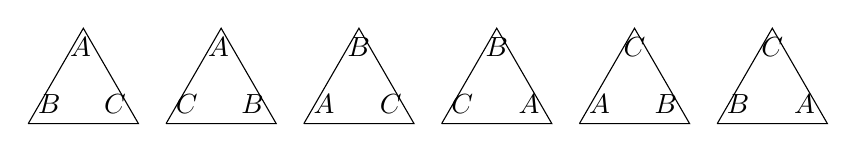
\begin{tikzpicture}[scale=0.7]
        \draw (-1,0)--(1,0)--(0,1.732)--(-1,0);
        \draw (-3.5,0)--(-1.5,0)--(-2.5,1.732)--(-3.5,0);
        \draw (-6,0)--(-4,0)--(-5,1.732)--(-6,0);
        \draw (4,0)--(6,0)--(5,1.732)--(4,0);
        \draw (1.5,0)--(3.5,0)--(2.5,1.732)--(1.5,0);
        \draw (6.5,0)--(8.5,0)--(7.5,1.732)--(6.5,0);
        \node[below] at (-5.05, 1.732) {$A$};
        \node[below] at (-2.55, 1.732) {$A$};
        \node[below] at (-0, 1.732) {$B$};
        \node[below] at (2.5, 1.732) {$B$};
        \node[below] at (5, 1.732) {$C$};
        \node[below] at (7.5, 1.732) {$C$};
        \node[above right] at (-6,0) {$B$};
        \node[above right] at (-3.5,0) {$C$};
        \node[above right] at (-1,0) {$A$};
        \node[above right] at (1.5,0) {$C$};
        \node[above right] at (4,0) {$A$};
        \node[above right] at (6.5,0) {$B$};
        \node[above left] at (-4.05,0) {$C$};
        \node[above left] at (-1.55,0) {$B$};
        \node[above left] at (0.95,0) {$C$};
        \node[above left] at (3.45,0) {$A$};
        \node[above left] at (5.95,0) {$B$};
        \node[above left] at (8.45,0) {$A$};
      \end{tikzpicture}
    \end{center}
  \end{example}

  \begin{example}[Dihedral Group of Order 8]
    The group of rotations and reflections that preserve the structure of a square in $\mathbb{R}^2$. is called the Dihedral Group $\Dih(4)$. 

    \begin{figure}[H]
      \centering 
      \begin{tabular}{|c|c|c|c|c|c|c|c|c|}
        \hline
        & $e$ & $r$ & $r^2$ & $r^3$ & $f$ & $rf$ & $r^2f$ & $r^3f$ \\
        \hline
        $e$ & $e$ & $r$ & $r^2$ & $r^3$ & $f$ & $rf$ & $r^2f$ & $r^3f$ \\
        \hline
        $r$ & $r$ & $r^2$ & $r^3$ & $e$ & $rf$ & $r^2f$ & $r^3f$ & $f$ \\
        \hline
        $r^2$ & $r^2$ & $r^3$ & $e$ & $r$ & $r^2f$ & $r^3f$ & $f$ & $rf$ \\
        \hline
        $r^3$ & $r^3$ & $e$ & $r$ & $r^2$ & $r^3f$ & $f$ & $rf$ & $r^2f$ \\
        \hline
        $f$ & $f$ & $r^3f$ & $r^2f$ & $rf$ & $e$ & $r^3$ & $r^2$ & $r$ \\
        \hline
        $rf$ & $rf$ & $f$ & $r^3f$ & $r^2f$ & $r$ & $e$ & $r^3$ & $r^2$ \\
        \hline
        $r^2f$ & $r^2f$ & $rf$ & $f$ & $r^3f$ & $r^2$ & $r$ & $e$ & $r^3$ \\
        \hline
        $r^3f$ & $r^3f$ & $r^2f$ & $rf$ & $f$ & $r^3$ & $r^2$ & $r$ & $e$ \\
        \hline
      \end{tabular}
      \caption{Multiplication table for $D_4$ using simplified notation.} 
      \label{fig:square_d4_simplified}
    \end{figure}

    Note that this is \textbf{not} the same as the symmetry group of the regular tetrahedron! 
  \end{example} 

  Following this pattern, we can extrapolate to find that the Dihedral group is a symmetry group. 

  \begin{theorem}[Dihedral Groups as Symmetry Groups]
    $\Dih(n)$ is similarly the group of all rotations and reflections that preserve the structure of a regular $n$-gon in $\mathbb{R}^2$. 
  \end{theorem}

  \begin{example}[Groups of Order 3]
    $\Dih(3) \simeq S_{3}$, since permutations of the vertices of a triangle are isomorphic to a permutations of a 3-element set. 
  \end{example}  

  \begin{theorem}[Tip]
    To prove a group homomorphism, show that every element of $G$ and $H$ can be written as a word of certain $g_i$'s in $G$ and then $h_i$'s in $H$, and map the $g_i$'s to $h_i$'s. 
  \end{theorem}

\subsection{Symmetric and Alternating Groups}

  We have seen the natural construction of the symmetric group of a set as the set of bijective transformations. Now the reason that symmetric groups are nice is that we can embed a group into its symmetric group. 

  \begin{theorem}[Cayley's Theorem]
    This applies for both monoids and groups. 
    \begin{enumerate}
      \item Any monoid is isomorphic to a monoid of transformations, i.e. there exists an injective monoid homomorphism 
        \begin{equation}
          f: M \to M^M
        \end{equation}
      \item Any group is isomorphic to a group of transformations, i.e. there exists an injective group homomorphism
        \begin{equation}
          f: G \to \Sym(G)
        \end{equation}
    \end{enumerate}
  \end{theorem}
  \begin{proof}
    Let $(M, \cdot, 1)$ be a monoid. Then we will construct a homomorphism $f: M \to M^M$, the monoid of transformations from $M$ to itself. For any $a \in M$, we define the \textit{left translation} $a_L : x \mapsto ax$. We claim that the set $M^\prime \coloneqq \{a_L \in M^M \mid a \in M \}$ is indeed a monoid. 
    \begin{enumerate}
      \item \textit{Closure}. Given $a, b \in M$, $ab \in M$ and so $ab_L \in M^\prime$. But $(ab_L)(x) = (ab)x = a (bx) = a_L (bx) = a_L (b_L (x)) = (a_L \circ b_L)(x)$, so $ab_L = a_L \circ b_L$. 
      \item \textit{Identity}. $e \in M \implies e_L \in M$ where $e_L : x \mapsto x$. 
    \end{enumerate}
    Next we claim that is is an isomorphism. 
    \begin{enumerate}
      \item This is a homomorphism due to the closure and identity properties proved above. 
      \item It is injective since given $a \neq b$ in $M$, $a_L$ and $b_L$ acts on the identity in different ways $a_L(e) = a \neq b = b_L (e)$, so $a_L \neq b_L$. 
      \item It is surjective by definition. 
    \end{enumerate}
    We have proved for monoids. For groups, we have the additional assumption that inverses exist in $G$, and we must prove that the set of left translations $G^\prime$ is indeed a group. It suffices to prove that inverses exist in $G^\prime$. Given $a \in G$, $a_L \in G^\prime$. But $a^{-1} \in G$ since $G$ is a group, and so $a^{-1}_L \in G^\prime$ as well. We can see that 
    \begin{align}
      (a^{-1}_L a_L) (x) & = (a^{-1} a) x = ex = x \\
      (a_L a^{-1}_L) (x) & = (a a^{-1}) x = ex = x
    \end{align}
    and so indeed $(a^{-1})_L = (a_L)^{-1}$. From this additional fact all the rest follows exactly as for monoids. 
  \end{proof}

  \begin{corollary}[Cayley]
    Every group $G$ is isomorphic to a subgroup of its symmetric group. 
  \end{corollary}

  Now we limit our scope to only finite sets, i.e. finite symmetric groups, which are often called \textbf{permutation} groups. For such finite sets the labeling does not matter since such groups are always isomorphic, so we can say $S = \{1, 2, \ldots, n\}$.

  \begin{theorem}[Symmetric Group as a Symmetry Group]
    The symmetric group $S_n$ is isomorphic to the symmetry group of the $n$-simplex in $\mathbb{R}^{n-1}$. 
  \end{theorem}
  \begin{proof}
    
  \end{proof}

  Now armed with group presentations and generating sets, let attempt to find a group presentation for a permutation group. Given set $S = \{1, 2, \ldots, n\}$, a permutation $\gamma \in \Sym(S)$ is denoted 
  \begin{equation}
    \gamma = \begin{pmatrix} 
      1 & 2 & 3 & 4 & \ldots & n-2 & n-1 & n \\ 
      i_1 & i_2 & i_3 & i_4 & \ldots & i_{n-2} & i_{n-1} & i_n 
    \end{pmatrix} \in \Sym(S)
  \end{equation} 

  We begin by introducing a specific instance of a permutation. 

  \begin{definition}[Cycle Permutation]
    A permutation is said to be \textbf{cyclic} if there exists some subset $A \subset S$ such that $\gamma$ acts as 
    \begin{equation}
      a_1 \mapsto a_2 \mapsto a_3 \ldots \mapsto a_k \mapsto a_1
    \end{equation}
    and leaves the rest unchanged. The notation for this is 
    \begin{equation}
      \begin{pmatrix} a_1 & a_2 & \ldots & a_k \end{pmatrix} \in \Sym(S)
    \end{equation}
    A cycle acting on a subset of 2 elements, i.e. a swap of two elements, is called a \textbf{transposition}. Two cyclic rotations $\gamma_1, \gamma_2$ are \textbf{disjoint} if the subsets that they act on are disjoint: $A \cap B = \emptyset$. 
  \end{definition}

  \begin{example}[Some Cyclic Permutations]
    This notation can be a bit weird, so let's give some simple examples. 
    \begin{enumerate}
      \item $(1 2)$ is a mapping $1 \rightarrow 2,\; 2 \rightarrow 1$. 
      \item $(1 2 3)$ is a mapping $1\rightarrow 2,\; 2 \rightarrow 3,\; 3 \rightarrow 1$. 
      \item $(1 2 3) (4 5)$ is a mapping $1\rightarrow 2,\; 2 \rightarrow 3,\; 3 \rightarrow 1, \;4 \rightarrow 5, \;5 \rightarrow 4$. 
    \end{enumerate}
  \end{example}

  \begin{lemma}
    Every element in finite $S_{n}$ can be decomposed into a partition of cyclic permutations.
  \end{lemma}

  \begin{example}[Cyclic Decomposition of Permutation]
    For the following permutation
    \begin{equation}
      \gamma = \begin{pmatrix} 
        1 & 2 & 3 & 4 & 5 & 6 & 7 & 8 \\ 
        3 & 6 & 5 & 4 & 8 & 2 & 7 & 1 
      \end{pmatrix} = (7)(4)(26)(1358)
    \end{equation} 
  \end{example}

  \begin{theorem}[Transpositions]
    The set of all transpositions forms a generating set of $S_{n}$. 
  \end{theorem}

  Recognizing that the set of transpositions is the generating set of the permutation group. In fact, transpositions allow us talk about the parity of an arbitrary permutation, through its signature. 

  \begin{definition}[Signature]
    The \textbf{signature} of a permutation is a homomorphism
    \begin{equation}
      \sign : S_{n} \longrightarrow \{1, -1\}
    \end{equation}
  \end{definition}

  \begin{lemma}
    The signature of a permutation changes for every transposition that is applied to it. 
  \end{lemma} 

  Now we are ready to introduce another fundamental type of group. 

  \begin{definition}[Alternating Group]
    The \textbf{alternating group} is the kernel of the signature homomorphism $\sign: S_n \to \{\pm 1\}$. 
    \begin{equation}
      A_n \coloneqq \ker{\sign}
    \end{equation}
    It is the set of even permutations with order $n!/2$.\footnote{Note that the set of odd permutations do not form a group, since the composition of two odd permutations (each having signature $-1$ is an even permutation. }
  \end{definition}

  This construction might seem arbitrarily specific to study so early into algebra, but as we will see later, we will find that that for $n \geq 5$, they will be simple groups that can't be decomposed and therefore fundamental in a sense. 

  \begin{example}[Low Order Symmetric Groups]
    \begin{enumerate}
      \item $S_{0}$ is the set of all permutations on the \textbf{null set}. $S_{1}$ is the set of all permutations on the \textbf{singleton set}. Both sets have cardinality 1 and the element is \textbf{trivial}. Note that $S_{1} = A_{1}$. 
      \item $S_{2}$ is a cyclic, abelian group of order 2 consisting of the identity permutation and the transposition of two elements. 
      \item $S_{3}$ is the first cyclic, nonabelian group, with order 6. $S \simeq \Dih(3)$, which can be seen as the group of rotations and reflections on the equilateral triangle, and the elements of $S_{3}$ equate to permuting the vertices on the triangle. 
    \end{enumerate}
  \end{example}

  In lecture, we talked about the number of all finite set is $e$. Since $n!$ is the order of permutation groups, i.e. the order of automorphism groups, we can sum their inverses over all $n \in \mathbb{N}$ to get $e$.  

\subsection{Group Actions} 

  We have studied the general properties of groups, but historically group theory arose from the study of transformation groups (which is why I also introduced is so early on). These transformation groups can be thought of as an abstract group it itself, but another way to interpret it is to see how it \textit{acts} on a set. 

  \begin{definition}[Group Action]
    Let $G$ be a group, $S$ a set. Then, a (left) group action of $G$ on $S$ is a function
    \begin{equation}
      \sigma: G \times S \to S, \qquad \sigma(g, a) = g \cdot a 
    \end{equation}
    satisfying two axioms. 
    \begin{enumerate}
      \item \textit{Identity}. $\forall a \in S, \sigma(e, a) = a$. 
      \item \textit{Compatibility}. $\forall g, h \in G \text{ and } \forall x \in X, \sigma(gh, x) = \sigma(g, \sigma(h, x))$.
    \end{enumerate}
    The group $G$ is said to \textbf{act on} $S$, and the evaluation $\sigma(g, a)$ can be interpreted as the result after transforming $a$ through $g$. 
  \end{definition}
  
  \begin{theorem}[Group Action as a Homomorphism onto the Symmetric Group]
    We have the immediate facts. 
    \begin{enumerate}
      \item For a fixed $g \in G$, the group action $\sigma_g (s) \coloneqq \sigma(g, s): S \to S$ is a bijection, i.e. an element of $\Sym(S)$. The inverse is the function mapping $x \mapsto \sigma(g^{-1}, x)$.
      \item The map from $G$ to $\Sym(S)$ defined by $g \mapsto \sigma_g$ is a homomorphism. 
    \end{enumerate}
  \end{theorem}
  \begin{proof}
    
  \end{proof}

  \begin{example}[Permutations and Dihedral Groups as Group Actions]
    In fact, we have seen two concrete examples of such group actions. 
    \begin{enumerate}
      \item The permutation group acts on the set $S = \{1, \ldots, n\}$ by permuting its elements. It also acts on a set of $n$-simplexes by rotating/flipping them. 
      \item The dihedral group acts on the set of regular $n$-gons by rotating/flipping them. 
    \end{enumerate}
  \end{example}



\section{Subgroups} 

  We have seen a few examples of subgroups, but we will heavily elaborate on here. We know that given a set, we can define an equivalence relation on it to get a quotient set. Now if we have a group, defining any such equivalence relation may not be compatible with the group structure. Therefore, it would be nice to have some principles in which we can construct such compatible equivalence classes, i.e. through a \textbf{congruence relation} that preserves the operations. 

  We introduce some standard notation. 

  \begin{definition}[Subgroup of Integer Multiples]
    The set $k \mathbb{Z}$ is the set of all integer multiples of $k$. This is a group under addition. 
  \end{definition}

\subsection{Cosets}

  Fortunately, we can do such a thing by taking a subgroup $H \subset G$ and ``shifting'' it to form the cosets of $G$, which are the equivalence classes. 
  
  \begin{definition}[Coset]
    Given a group $G$, $a \in G$, and subgroup $H$, 
    \begin{enumerate}
      \item A \textbf{left coset} is $a H \coloneqq \{a h \mid h \in H \}$. 
      \item A \textbf{right coset} is $H a \coloneqq \{h a \mid h \in H \}$. 
      \item When $G$ is abelian, the \textbf{coset} is denoted $a + H$. 
    \end{enumerate}
    With this, we can take arbitrary elements $a, b \in G$ and determine if they are in the same coset as such. Since $a \in aH$, $b \in aH$ iff $b = ah$ for some $h \in H$. Therefore, we have the equivalence relation. 
    \begin{equation}
      a \equiv b \pmod{H} \iff a = b h \text{ for some } h \in H
    \end{equation}
  \end{definition}
  \begin{proof}
    We show that this indeed forms an equivalence class. 
    \begin{enumerate}
      \item \textit{Reflexive}. $a \equiv a \pmod{H}$ since $e \in H \implies a = a e$. 
      \item \textit{Symmetric}. Let $a \equiv b \pmod{H}$. Then $a = bh$ for some $h \in H$, but since $H$ is a group, $h^{-1} \in H \implies a h^{-1} = b \implies b \equiv a \pmod{H}$. 
      \item \textit{Transitive}. Let $a \equiv b \pmod{H}$ and $b \equiv c \pmod{H}$. Then $a = bh$ and $b = ch^\prime$ for some $h, h^\prime \in H$. But then 
      \begin{equation}
        a = bh = (ch^\prime) h = c(h^\prime h)
      \end{equation}
      where $h^\prime h \in H$ due to closure. 
    \end{enumerate}
  \end{proof} 

  Note that a coset is \textit{not} a subgroup. It is only the case that $eH = H$ is a subgroup, but for $a \neq e$, $aH$ does not even contain the identity. We should think of a coset as a \textit{translation} of the subgroup $H$. 

  \begin{example}[Familiar Cosets]
    Here are some examples. Note that all it takes is to find \textit{some} subgroup, and the cosets will naturally pop up. 
    \begin{enumerate}
      \item Let $H = 2 \mathbb{Z} \subset (\mathbb{Z}, +)$ be the even integers. Then $0 + H$ and $1 + H$ are the even and odd integers, respectively. 
      \item Let $H = \{e, f\} \subset \Dih(3)$. Then 
      \begin{equation}
        H = \{e, f\}, rH = \{r, rf\}, r^2 H = \{r^2, r^2 f\} 
      \end{equation}
      are the cosets. 
    \end{enumerate}
  \end{example}

  With this partitioning scheme in mind, the following theorem on the order of such groups becomes very intuitive, and has a lot of consequences. 

  \begin{theorem}[Lagrange's Theorem]
    Let $G$ be a finite group and $H$ its subgroup. Then 
    \begin{equation}
      |G| = [G:H] |H|
    \end{equation}
    where $[G:H]$, called the \textbf{index of $H$}, is the number of cosets in $G$. Therefore, the order of a subgroup of a finite group divides the order of the group. 
  \end{theorem}
  \begin{proof}
    The union of the $[G:H]$ disjoint cosets is all of $G$. On the other hand, every $H$ is in one-to-one correspondence with each coset $aH$, so every coset has $|H|$ elements. Therefore, there are $[G:H] |H|$ elements altogether. 
  \end{proof}

  Therefore, Lagrange's theorem says that \textit{given} that you find a subgroup, the order of the subgroup must divide the order of $G$. However, that doesn't mean that such a subgroup may even exist. For example, there is a group of order 12 having no subgroup of order 6. 

  \begin{corollary}
    The order of any element of a finite group divides the order of the group. 
  \end{corollary}
  \begin{proof}
    Take any $a \in G$ and construct the cyclic subgroup $\langle a \rangle \subset G$. Then by Lagrange's theorem, $|a| = |\langle a \rangle|$ divides $|G|$. 
  \end{proof}

  \begin{corollary}
    Every finite group of a prime order is cyclic. 
  \end{corollary}
  \begin{proof}
    Let $a \in G$ be any element other than the identity $e$, and consider $\langle a \rangle \subset G$. The order must divide $|G|$ which is prime, so $|a| = 1$ or $|G|$. But $|a| \neq 1$ since we did not choose the identity, so $|a| = |G| \implies \langle a \rangle = G$. 
  \end{proof}

  \begin{corollary}
    If $|G| = n$, then for every $a \in G$ $a^n = e$. 
  \end{corollary}
  \begin{proof}
    Let $|a| = k$. Then $k \mid n$, and so $a^n = a^{kl} = (a^k)^l = e^l = e$. 
  \end{proof}

  \begin{corollary}[Fermant's Little Theorem]
    Let $p$ be a prime number. The multiplicative group $\mathbb{Z}_{p} \setminus \{0\}$ of the field $\mathbb{Z}_{p}$ is an abelian group of order $p-1 \implies g^{p-1} = 1$ for all $g \in \mathbb{Z}_{p} \setminus \{0\}$. So,
    \begin{equation}
      a^{p-1} \equiv 1 \iff a^{p} \equiv a \pmod{p}
    \end{equation}
  \end{corollary} 

  We can generalize this. 

  \begin{definition}[Euler's Totient Function]
    \textbf{Euler's Totient Function}, denoted $\varphi(n)$, consists of all the numbers less than or equal to $n$ that are coprime to $n$. 
  \end{definition}

  \begin{theorem}[Euler's Theorem]
    For any $n$, the order of the group $\mathbb{Z}_{n} \setminus \{0\}$ of invertible elements of the ring $\mathbb{Z}_{n}$ equals $\varphi(n)$, where $\varphi$ is Euler's totient function. In other words with $G = \mathbb{Z}_{n} \setminus \{0\}$, 
    \begin{equation}
      a^{\varphi(n)} \equiv 1 \pmod{n}, \; \text{ where $a$ is coprime to $n$}
    \end{equation}
  \end{theorem}

  \begin{example}
    In $\mathbb{Z}_{125} \setminus \{0\}$, $\varphi(125) = 125 - 25 = 100 \implies 2^{100} \equiv 1 \pmod{125}$
  \end{example}

\subsection{Normal Subgroups}

  By introducing cosets, we have successfully constructed an equivalence relation on $G$. This set of cosets is indeed a partition of $G$, but we would like to endow it with a group structure that respects that of $G$. That is, let $a, b \in G$ and its corresponding cosets be $aH, bH$. Then, we would like to define an operation $\cdot$ on the cosets such that 
  \begin{equation}
    (aH) \cdot (bH) \coloneqq (ab)H
  \end{equation} 
  That is, we would like to upgrade the equivalence relation to a \textit{congruence relation}. If we try to show that this is indeed a well-defined operation, we run into some trouble. Suppose $aH = a^\prime H$ and $bH = b^\prime H$. Then with our definition, we should be able to derive that $(aH)(bH) = (a^\prime H) (b^\prime H)$ through the equation 
  \begin{equation}
     (aH) (bH) = (ab)H = (a^\prime b^\prime) H = (a^\prime H) (b^\prime H) 
  \end{equation}
  We have $a^\prime = a h_1$, $b^\prime = b h_2$, and $a^\prime b^\prime = ab h$. Then, 
  \begin{align}
    (ab) H = (a^\prime b^\prime) H & \implies a^\prime b^\prime = abh \text{ for some } h \in H \\
                                   & \implies a h_1 b h_2 = abh \text{ for some } h_1, h_2, h \in H
  \end{align}
  But the final statement is not true in general. In an abelian group, we could just swap $h_1$ and $b$ to derive it completely, but perhaps there is a weaker condition on just the subgroup $H$ that allows us to ``swap'' the two. 

  \begin{definition}[Normal Subgroups]
    A subgroup $N \subset G$ is a \textbf{normal subgroup} iff the left cosets equal the right cosets. That is, $\forall g \in G, h \in H$. 
    \begin{equation}
      g^{-1} h g \in H
    \end{equation}
    We call $g^{-1} h g$ the \textbf{conjugate} of $h$ by $g$. 
  \end{definition} 

  \begin{example}[Normal Subgroups]
    For intuition, we provide some examples of normal subgroups. 
    \begin{enumerate}
      \item If $G$ is abelian, every subgroup is normal. So $(2\mathbb{Z}, +)$ is normal, and $(\mathbb{Q}, \times) \subset (\mathbb{R}, \times)$ is also normal. 
      \item Given $G = (\mathbb{R} \setminus \{0\}, \times)$, let $H = (\mathbb{R}^+, \times) \subset G$ be a subgroup. Then $H$ is normal since for any $g \in \mathbb{R}$, $g, g^{-1}$ are either both positive or both negative, and so $g h g^{-1} > 0 \implies g h g^{-1} \in H$. $H$ and $(-1)H$ are two cosets of $\mathbb{R}$. 
      \item $\SL_n (\mathbb{F}) \subset \GL_n (\mathbb{F})$ is a normal subgroup since the determinant of the inverse is ihe inverse of the determinant, and so for any $g \in \GL_n (\mathbb{F})$, 
      \begin{equation}
        \det(g h g^{-1}) = \det(g) \det(h) = \det(g^{-1}) = \det(g) \cdot 1 \cdot \frac{1}{\det(g)} = 1 \implies g h g^{-1} \in \SL_n (\mathbb{F}) 
      \end{equation}

      \item The subgroup $H = \{e, r^2\} \subset \Dih(4)$ is a normal subgroup. It is clearly a subgroup isomorphic to $Z_2$, and to see normality, note that $r^2$ commutes with any $g = r^n \in \Dih(4)$. If $g$ contains a flip, then we can just check the 4 cases knowing that $f r = r^3 f$. 
      \begin{align}
        f r^2 f^{-1} & = f r^2 f = (f r)(r f) = r^3 f r f = r^3 r^3 f^2 = r^2 \\ 
        (rf) r^3 (rf)^{-1} & = \ldots = r^2
      \end{align}
      Therefore $\Dih(4)/H$ has order 4, which means it must be isomorphic to either the cyclic group or the Klein 4 group. It turns out it's the Klein 4 group. 
    \end{enumerate}
  \end{example}

  \begin{example}[Subgroups that are Not Normal]
    Here are some subgroups that are not normal. 
    \begin{enumerate}
      \item Given $G = \Dih(3)$, $H = \{e, f\}$ is not normal since $rf r^{-1} = r f r^2 = r^2 f \not\in H$. 
      \item The subgroup 
      \begin{equation}
        H = \bigg\{ \begin{pmatrix} a & b \\ 0 & c \end{pmatrix} \; \bigg| \; ac \neq 0 \bigg\} \subset \GL_2 (\mathbb{R})
      \end{equation} 
      is not normal since 
      \begin{equation}
        h = \begin{pmatrix} 1 & 1 \\ 0 & 1 \end{pmatrix} \in H , a = \begin{pmatrix} 1 & 0  \\ 1 & 1 \end{pmatrix} \in \GL_2 (\mathbb{R}) \implies a h a^{-1} = \begin{pmatrix} 0 & 1 \\ -1 & 2 \end{pmatrix} \not\in H
      \end{equation}
    \end{enumerate}
  \end{example}

  Finally, we present some relevent results of alternating subgroups. 

  \begin{theorem}[Alternating Group is Normal in Symmetric]
    $A_n$ is a normal subgroup of $S_n$, of index\footnote{i.e. the number of cosets} $2$. 
  \end{theorem}
  \begin{proof}
    
  \end{proof} 

  \begin{lemma}[Cycles in Alternating Group]
    \label{thm:cycles_alt}
    We have the following. 
    \begin{enumerate}
      \item Every element of $A_n$ can be written as the product of 3-cycles. 
      \item If $n \geq 4$, $H$ is a normal subgroup of $A_n$, and $H$ contains one 3-cycle, then $H = A_n$. 
    \end{enumerate}
  \end{lemma}
  \begin{proof}
    Since we've proved that every permutation is the product of transpositions, it suffices to prove that the product of two transpositions can be written as the product of 3-cycles. We check this case by case, where distinct symbols represent distinct values. 
    \begin{enumerate}
      \item $(\alpha \; \beta) ( \gamma \; \delta) = (\alpha \; \beta \; \gamma) (\beta \; \gamma \; \delta)$ 
      \item $(\alpha \; \beta)(\alpha \; \gamma) = (\alpha \; \gamma \; \beta)$ 
      \item $(\alpha \; \beta) (\alpha \; \beta) = e$
    \end{enumerate}
    Therefore every even permutation is the product of 3-cycles. 
  \end{proof}

  \begin{definition}[Simple Group]
    A \textbf{simple group} is a group with no proper normal subgroup. That is, the only normal subgroups are the trivial group and itself. 
  \end{definition}

  \begin{theorem}[Alternating Groups are Simple]
    For $n \geq 5$, $A_n$ is a simple group. 
  \end{theorem}
  \begin{proof}
    Let $H \subset A_n$ be a normal subgroup containing more than the identity. If we can find a single 3-cycle in $H$, then it follows from \ref{thm:cycles_alt} that $H = A_n$. Let $\gamma \in H$, $\gamma \neq e$, and write $\gamma = \gamma_1 \ldots \gamma_m$ as a product of disjoint cycles. We have 4 cases. 
    \begin{enumerate}
      \item Let $k \geq 4$ and suppose that some factor, say $\gamma_1$ is a $k$-cycle. WLOG let us assume that $\gamma_1 = (1 \ldots k)$. Since $H$ is normal, $(1, 2, 3) \gamma (1, 2, 3)^{-1} \in H$ and $(1, 2, 3)$ commutes with all the factors of $\gamma$ except $\gamma_1$ (since the cycles are disjoint and so $\gamma_i$ for $i \neq 1$ does not contain $1, 2, 3$). Thus letting 
      \begin{equation}
        \sigma = (1, 2, 3) \gamma (1, 2, 3)^{-1} = (2, 3, 1, 4, \ldots, k) \gamma_2 \ldots \gamma_m \in H
      \end{equation} 
      since $H$ is a group we have 
      \begin{align}
        \sigma \gamma^{-1} & = \begin{pmatrix} 2 & 3 & 1 & 4 \ldots & k \end{pmatrix} \begin{pmatrix} 1 & 2 & 3 & 4 & \ldots & k \end{pmatrix}^{-1} \\
                           & = \begin{pmatrix} 2 & 3 & 1 & 4 & \ldots & k \end{pmatrix} \begin{pmatrix} k & \ldots & 4 & 3 & 2 & 1 \end{pmatrix} = \begin{pmatrix} 1 & 2 & 4 \end{pmatrix}
      \end{align}

      \item Suppose $\gamma$ has at least two 3-cycles as factors, say $\gamma_1 = (1, 2, 3), \gamma_2 = (4, 5, 6)$. Then 
      \begin{equation}
        \sigma = (3, 4, 5) \gamma (3, 4, 5)^{-1} = (1, 2, 4) (3, 6, 5) \gamma_3 \ldots \gamma_m \in H
      \end{equation}
      and again we have 
      \begin{align}
        \sigma \gamma ^{-1} & = 
        \begin{pmatrix} 1 & 2 & 4 \end{pmatrix}
        \begin{pmatrix} 3 & 6 & 5 \end{pmatrix}
        \begin{pmatrix} 4 & 5 & 6 \end{pmatrix}^{-1}
        \begin{pmatrix} 1 & 2 & 3 \end{pmatrix}^{-1} \\ 
                          & = \begin{pmatrix} 1 & 6 & 3 & 4 & 5 \end{pmatrix}
      \end{align}
      which is a 5-cycle, and we are done by case 1. 

      \item Suppose $\gamma$ has precisely one 3-cycle factor and all others are transposisions. If the 3-cycle is $\gamma_1 = (1, 2, 3)$, then $\gamma^2 = (1, 2, 3)^2 = (1, 3, 2)$ is a $3$-cycle. 

      \item Suppose $\gamma$ is the product of disjoint transpositions. Say $\gamma_1 = (1, 2), \gamma_2 = (3, 4)$. Then as before 
      \begin{equation}
        \sigma = \begin{pmatrix} 1 & 2 & 4 \end{pmatrix} \gamma \begin{pmatrix} 1 & 2 & 4 \end{pmatrix}^{-1}  \implies \sigma \gamma^{-1} = \begin{pmatrix} 1 & 4 \end{pmatrix} \begin{pmatrix} 2 & 3 \end{pmatrix} \in H
      \end{equation}
      Since $n \geq 5$ by our theorem hypothesis, the permutation $\tau = (2, 3, 5) \in A_n$, and so 
      \begin{align}
        \tau \begin{pmatrix} 1 & 4 \end{pmatrix} \begin{pmatrix} 2 & 3 \end{pmatrix} \tau^{-1} & = \begin{pmatrix} 1 & 4 \end{pmatrix} \begin{pmatrix} 3 & 5 \end{pmatrix} \in H \\
            \implies & \begin{pmatrix} 1 & 4 \end{pmatrix} \begin{pmatrix} 2 & 3 \end{pmatrix} \begin{pmatrix} 1 & 4 \end{pmatrix} \begin{pmatrix} 3 & 5 \end{pmatrix} = \begin{pmatrix} 2 & 5 & 3 \end{pmatrix} \in H
      \end{align}
    \end{enumerate}
  \end{proof}

\subsection{Quotient Groups}

  Now that we know about normal subgroups, this allows us to endow on the quotient set a group structure. 

  \begin{definition}[Quotient Group]
    Given a group $G$ and a normal subgroup $H$, the \textbf{quotient group} $G/H$ is the group of left cosets $aH$ with 
    \begin{enumerate}
      \item the operation $(aH) \cdot (bH) \coloneqq (ab)H$ 
      \item the identity element $eH$. 
      \item inverses $(aH)^{-1}) = (a^{-1})H$. 
    \end{enumerate}
    and order $|G/H| = |G| / |H|$.  
  \end{definition}
  \begin{proof}
    We verify the properties of a group. 
    \begin{enumerate}
      \item Suppose as above that $aH = a^\prime H$ and $bH = b^\prime H$. Then $a^\prime = ah$ and $b^\prime = bk$ for some $h, k \in H$. Since $H$ is normal, $b^{-1} h b = h^\prime$ for some $h^\prime \in H$. Therefore, 
      \begin{equation}
        a^\prime b^\prime = (ah) (bk) = a(hb) k = (ab h^\prime) k = (ab)(h^\prime k) \in (ab) H
      \end{equation}
      and so $(ab)H = (a^\prime b^\prime)H$. 

      \item $eH$ is indeed the identity since $(aH)(eH) = (ae)H = aH$ and $(eH)(aH) = (ea)H = aH$. 
      \item Inverses are the same logic. 
      \item Associativity follows from associativity in $G$. 
    \end{enumerate}
    Finally, by Lagrange's theorem, the order is as stated. 
  \end{proof}

  Since the quotient defines a \textit{congruence} class, this makes it a group homomorphism. 

  \begin{theorem}[Quotient Maps are Homomorphisms]
    The map $p: G \rightarrow G/H$ is a group homomorphism. 
  \end{theorem}
  \begin{proof}
    Follows immediately from the definition. 
  \end{proof} 

  It's a bit hard thinking of an intuitive picture of a normal subgroup. Unless you sit down and try to prove that a subgroup is normal, it's difficult to tell right away. The following lemma characterizes normal subgroups in a different manner. 

  \begin{lemma}[Normal Subgroup as Kernel]
    \label{thm:normal_kernel}
    A subgroup $H \subset G$ is normal if and only if there exists a group homomorphism $\phi: G \rightarrow G^\prime$ with $\ker{\phi} = H$. 
  \end{lemma}
  \begin{proof}
    We prove bidirectionally. 
    \begin{enumerate}
      \item $(\rightarrow)$. Since $H$ is normal, we can form the quotient group $G/H$. Let $\phi: G \rightarrow G/H$ be defined $\phi(a) = aH$. Then, 
      \begin{align}
        \ker{\phi} = \phi^{-1}(eH) & = \{a \in G \mid aH = eH = H \} \\
                                   & = \{a \in G \mid a \in H \}
      \end{align}
      Therefore, $\phi$ is a homomorphism because $\phi(ab) = abH = (aH)(bH)$.   

      \item $(\leftarrow)$ Assume there is a group homomorphism $\phi$. Then, $\ker{\phi} \subset G$ is a subgroup proven in \ref{thm:kernels_subgroup}. Now consider any $g \in G$. Then 
      \begin{equation}
        \phi(g h g^{-1}) = \phi(g) \phi(h) \phi(g^{-1}) = \phi(g) \cdot e \cdot \phi(g)^{-1} = e \implies g h g^{-1} \in \ker{\phi}
      \end{equation}
    \end{enumerate}
  \end{proof}

  Now that we can construct quotient groups, we would like to see if they are isomorphic to any current groups that we know. More specifically, if we have a normal subgroup $H \subset G$, we can cleverly think of some other group $G^\prime$ and construct a group homomorphism $f: G \to G^\prime$ such that $H = \ker{f}$. If we can do this, then we can construct a nice isomrophism from $G/H$ to $G^\prime$. 

  \begin{theorem}[Fundamental Group Homomorphism Theorem]
    Let $f: G \to G^\prime$ be a surjective homomorphism.\footnote{Sometimes called an \textit{epimorphism}.} Then $G/{\ker{f}} \simeq G^\prime$.\footnote{Note that if $f$ is not surjective, we can just have it be surjective by restricting $G^\prime$ to be the image of $f$. }

    \begin{figure}[H]
      \centering 
      \begin{tikzcd}
        G \arrow[r, "f"] \arrow[d, "p"] & G' \\
        G/\ker{f} \arrow[ur, "\bar{f}"'] &
      \end{tikzcd}
      \caption{Given $f$ and the projection map $p: G \to G/{\ker{f}}$, this induces an isomorphism $\bar{f}$ such that $f = \bar{f} \circ p$.} 
      \label{fig:group_fund_homo_theorem}
    \end{figure}
  \end{theorem}
  \begin{proof}
    Let $H = \ker{f}$, which is then a normal subgroup from \ref{thm:normal_kernel}. Now we define a homomorphism 
    \begin{equation}
      \bar{f}: G/H \to G^\prime, \qquad \bar{f}(aH) = f(a)
    \end{equation}
    We check the following. 
    \begin{enumerate}
      \item $\bar{f}$ is well defined. If we have $a, a^\prime \in G$ with $aH = a^\prime H$, then $a^\prime = a h$ for some $h \in H = \ker{f}$. So $f(a^\prime) = f(ah) = f(a) f(h) = f(a)$. 

      \item $\bar{f}$ is a homomorphism. We see that 
      \begin{align}
        \bar{f}((aH)(bH)) & = \bar{f}((ab)H) \\ 
                          & = f(ab) \\
                          & = f(a) f(b) \\  
                          & = \bar{f}(aH) \bar{f}(bH) 
      \end{align}

      \item $\bar{f}$ is surjective. This is trivially true since if not, then $f = \bar{f} \circ p$ cannot be surjective. 

      \item $\bar{f}$ is injective. By \ref{thm:kernels_subgroup}, it suffices to show that $\ker{\bar{f}}$ is trivial. Suppose $aH \in \ker{\bar{f}}$. Then $\bar{f}(aH) = f(a) = e_{G^\prime} \implies a \in H \implies aH = eH$. 
    \end{enumerate}
  \end{proof}

  \begin{example}[Cyclic Groups]
    $(k \mathbb{Z}, +) \subset (\mathbb{Z}, +)$ is a normal subgroup. Our intuition might tell us that the cosets of the form $k \mathbb{Z}, 1 + k \mathbb{Z}, \ldots, (k-1) + k\mathbb{Z}$ behave like integers modulo $k$, i.e. a cyclic group. Therefore, we can construct the map 
    \begin{equation}
      f: \mathbb{Z} \to Z_k, \qquad f(x) = x \pmod{k}
    \end{equation} 
    This is a homomorphism and also $\ker{f} = k \mathbb{Z}$, and so by the fundamental homomorphism theorem 
    \begin{equation}
      \frac{\mathbb{Z}}{k \mathbb{Z}} \simeq Z_k 
    \end{equation}
    By establishing the connection between the integers and cyclic groups, we establish the notation $Z_k = \mathbb{Z}_k$. 
  \end{example}

  \begin{example}[Quotient of Reals over Integers]
    We can see that $(\mathbb{Z}, +) \subset (\mathbb{R}, +)$ is a normal subgroup. Our intuition might tell us that the cosets (which are disconnected sets consisting of isolated points $\{\ldots, x - 1, x, x + 1, \ldots\}$) behave sort of like the rotations on a circle $S^1$. Therefore, let us construct a map 
    \begin{equation}
      f: \mathbb{R} \to S^1, \qquad f(x) = \cos{2\pi x} + i \sin{2\pi x} \subset \mathbb{C}
    \end{equation}
    Since $f(x + y) = f(x) f(y)$, it follows that $f$ is a homomorphism. On the other hand, $\ker{f} = \{ x \in \mathbb{R} \mid \cos{2 \pi x} = 1, \sin{2 \pi x} = 0 \} = \mathbb{Z}$. Therefore by the fundamental homomorphism theorem, we have
     
    \begin{equation}
      \mathbb{R}/\mathbb{Z} \simeq S^1
    \end{equation}
  \end{example}

\subsection{Orbits and Stabilizers}

  \begin{definition}[Orbits]
    Let $G$ be a transformation group on set $X$. Points $x, y \in X$ are equivalent with respect to $G$ if there exists an element $g \in G$ such that $y = g x$. This has already been defined through the equivalence of figures before. This relation splits $X$ into equivalence classes, called \textbf{orbits}. Note that cosets are the equivalence classes of the transformation group $G$; oribits are those of $X$. We denote it as
    \begin{equation}
      Gx \equiv \{ g x \;|\;g \in G \}
    \end{equation}
  \end{definition}

  By definition, transitive transformation groups have only one orbit.

  \begin{definition}
    The subgroup $G_{x} \subset G$, where $G_{x} \equiv \{ g \in G | g x = x\}$ is called the \textbf{stabilizer} of $x$.
  \end{definition}

  \begin{example}
    The orbits of $O(2)$ are concentric circles around the origin, as well as the origin itself. The stabilizer of $0$ is the entire $O(2)$.
  \end{example}

  \begin{example}
    The group $S_n$ is transitive on the set $\{1, 2, ..., n\}$. The stabilizer of $k, (1 \leq k \leq n)$ is the subgroup $H_{k} \simeq S_{n-1}$, where $H_k$ is the permutation group that does not move $k$ at all. 
  \end{example}

  \begin{theorem}
    There exists a 1-to-1 injective correspondence between an orbit $G_x$ and the set $G / G_{x}$ of cosets, which maps a point $y = g x \in G x $ to the coset $g G_x$. 
  \end{theorem}

  \begin{corollary}
    If $G$ is a finite group, then 
    \begin{equation}
      |G| = |G_x| |G x|
    \end{equation}
    In fact, there exists a precise relation between the stabilizers of points of the same orbit, regardless of $G$ being finite or infinite: 
    \begin{equation}
      G_{g x} = g G_{x} g^{-1}
    \end{equation}
  \end{corollary}

\subsection{Centralizers and Normalizers} 

\subsection{Lattice of Subgroups} 


\section{Group Actions} 

\subsection{Sylow Theorems}


\section{Classification of Groups} 

\subsection{Direct Products}

  \begin{definition}[Direct Product]
    The \textbf{direct product} of two groups $G$ and $H$ is denoted
    \begin{equation}
      G \times H \equiv \{ (g, h)\;|\; g \in G, h \in H \}
    \end{equation}
    Note that the product need not be binary (nor must it be of finite arity). 
  \end{definition}

  \begin{example}
    The \textbf{general affine group} is defined 
    \begin{equation}
      \text{GA}(V) \equiv \text{Tran}\,V \times \text{GL}(V)
    \end{equation}
  \end{example}

  \begin{example}
    The \textbf{Galileo Group} is the transformation group of spacetime symmetries that are used to transform between two reference frames which differ only by constant relative motion within the constructs of Newtonian physics. It is denoted 
    \begin{equation}
      \text{Tran}\;\mathbb{R}^{4} \times H \times \text{O} (3)
    \end{equation}
    where $H$ is the group of transformations of the form 
    \begin{equation}
      (x, y, z, t) \longmapsto (x+at, y+bt, z+ct, t)
    \end{equation}
  \end{example}

  \begin{example}
    The \textbf{Poincaré Group} is the symmetry group of spacetime within the principles of relativistic mechanics, denoted
    \begin{equation}
      G = \text{Tran}\; \mathbb{R}^{4} \times \text{O}_{3,1}
    \end{equation}
    where O$_{3,1}$ is the group of linear transformations preserving the polynomial 
    \begin{equation}
      x^{2} + y^{2} + z^{2} - t^{2}
    \end{equation}
  \end{example} 

\subsection{Semidirect Products} 

\subsection{Classification of Finite Abelian Groups} 

  \begin{theorem}[Groups of Order 1, 2, 3]
    We have the following. 
    \begin{enumerate}
      \item There is only one group of order 1. 
        \begin{equation}
          Z_1 \simeq S_1 \simeq A_2
        \end{equation}

      \item There is only one group of order 2. 
        \begin{equation}
          Z_2 \simeq S_2 \simeq D_2
        \end{equation}

      \item There is only one group of order 3. 
        \begin{equation}
          Z_3 = A_3
        \end{equation}
    \end{enumerate}
  \end{theorem}

  \begin{theorem}[Groups of Order 4]
    There are two groups of order 4. 
    \begin{equation}
      Z_4, \qquad Z_2^2 \simeq D_4
    \end{equation}
  \end{theorem}

\subsection{Group Extensions}

\subsection{Classification of Simple Groups of Small Order}

  \begin{theorem}[Classification of Simple Groups of Small Order]
    The following are the only groups of order $n$. You can notice that it is dominated by direct products of cyclic groups, since they exist for every order, while the other types increase in order very fast.   

    \begin{figure}[H]
      \centering
      \begin{tabular}{|c|l|l|}
      \hline
      $n$ & \textbf{Abelian Groups} & \textbf{Non-Abelian Groups} \\
      \hline
      1 & $\{e\}$ (trivial group) & None \\
      \hline
      2 & $\mathbb{Z}_2 = S_2 = \text{Dih}(1)$ & None \\
      \hline
      3 & $\mathbb{Z}_3 = A_3$ & None \\
      \hline
      4 & $\mathbb{Z}_4$, $\mathbb{Z}_2 \times \mathbb{Z}_2 = \text{Dih}(2)$ & None \\
      \hline
      5 & $\mathbb{Z}_5$ & None \\
      \hline
      6 & $\mathbb{Z}_6 = \mathbb{Z}_3 \times \mathbb{Z}_2$ & $S_3 = \text{Dih}(3)$ \\
      \hline
      7 & $\mathbb{Z}_7$ & None \\
      \hline
      8 & $\mathbb{Z}_8$, $\mathbb{Z}_4 \times \mathbb{Z}_2$, $\mathbb{Z}_2 \times \mathbb{Z}_2 \times \mathbb{Z}_2$ & $D_4 = \text{Dih}(4)$, $Q_8$ (quaternion) \\
      \hline
      9 & $\mathbb{Z}_9$, $\mathbb{Z}_3 \times \mathbb{Z}_3$ & None \\
      \hline
      10 & $\mathbb{Z}_{10} = \mathbb{Z}_5 \times \mathbb{Z}_2$ & $D_5 = \text{Dih}(5)$ \\
      \hline
      11 & $\mathbb{Z}_{11}$ & None \\
      \hline
      12 & $\mathbb{Z}_{12} = \mathbb{Z}_4 \times \mathbb{Z}_3$, $\mathbb{Z}_6 \times \mathbb{Z}_2$, $\mathbb{Z}_2 \times \mathbb{Z}_2 \times \mathbb{Z}_3$ & $A_4$, $D_6 = \text{Dih}(6)$, $\mathbb{Z}_3 \rtimes \mathbb{Z}_4$ (dicyclic) \\
      \hline
      \end{tabular}
      \caption{Classification of groups up to order 12.}
      \label{tab:groups_up_to_order_10}
    \end{figure}
  \end{theorem}



\section{Rings} 

  \begin{definition}[Ring]
    A \textbf{ring} is a set $(R, +, \times)$ equipped with two operations, called addition and multiplication. It has properties: 
    \begin{enumerate}
      \item $R$ is an abelian group with respect to $+$, where we denote the additive identity as $0$ and the additive inverse of $x$ as $-x$. 
      \item $R$ is a monoid with respect to $\times$, where we denote the multiplicative identity as $1$, also known as the \textbf{unity}. 
      \item $\times$ is both left and right distributive with respect to addition $+$
      \begin{align}
        a \times (b + c) & = a\times b + a\times c \\ 
        (a + b) \times c & = a\times c + b\times c 
      \end{align}
      for all $a, b, c \in \mathbb{R}$. 
    \end{enumerate} 
    If $\times$ is associative, $R$ is called an \textbf{associative ring}, and if $\times$ is commutative, $R$ is called a \textbf{commutative ring}. 
  \end{definition}

  In fact, in some cases the existence of the multiplicative identity is not even assumed, though we will do it here.\footnote{If a multiplicative identity is not assumed, then this is called an \textit{rng}, or a \textit{rung}.}

  \begin{lemma} 
    Additive inverses are unique and $-1 \times a$ is the additive inverse of $a$. 
  \end{lemma}
  \begin{proof}
    We can see that 
    \begin{align}
      -1 + 1 = 0 & \implies (-1 + 1) \times a = 0 \times a \\
                 & \implies -1 \times a + 1 \times a = 0 \\
                 & \implies -1 \times a + a = 0 
    \end{align}
    and therefore by definition $-1 \times a$ must be the additive inverse. 
  \end{proof} 

  \begin{definition}[Characteristic Number]
    The \textbf{characteristic} of ring $R$, denoted char$(R)$, is the smallest number of times one must successively add the multiplicative identity $1$ to get the additive identity $0$. 
    \begin{equation}
      1 + 1 + ... + 1 = 0 
    \end{equation}
    If no such number $n$ exists, then char$(R) = 0$. 
  \end{definition}

  \begin{theorem}[Freshman's Dream]
    Given a field $F$ with char$(F) = p$, 
    \begin{equation}
      (a + b)^p = a^p + b^p
    \end{equation}
  \end{theorem}
  \begin{proof}
    We have 
    \begin{equation}
      (a + b)^p = \sum_{k = 0}^p \binom{p}{k} a^{p-k} b^{k}
    \end{equation}
    It is clear that 
    \begin{equation}
      \binom{p}{k} = \frac{p (p-1) ... (p - k+1)}{k!}
    \end{equation}
    is divisible by $p$ for all $k \neq 0, p$, so all the middle terms must cancel out to $0$. 
  \end{proof}


  Note that we do not assume that there exists multiplicative inverses in a ring. However, there may be some elements for which multiplicative inverses do exist, i.e. $a, b \in R$ where $ab = 1$.  

  \begin{definition}[Unit]
    A \textbf{unit} of a ring $R$ is an element $u \in R$ that has a multiplicative inverse in $R$. That is, there exists a $v \in R$ s.t. $uv = vu = 1$. 
  \end{definition}

  The next property that we would like to talk about is a zero divisor, which is the property that nonzero $a, b \in R$ satisfy $ab = 0$. 

  \begin{definition}[Left, Right Zero Divisor]
    An element $a$ of a ring $R$ is called a \textbf{left zero divisor} if there exists a nonzero $x$ such that $a x = 0$ and a \textbf{right zero divisor} if there exists a nonzero $x$ such that $x a = 0$. 
  \end{definition} 

  Another property that we would desire is some sort of decomposition of ring elements as other ring elements. 

  \begin{definition}[Left, Right Divisor]
    Let $a, b \in R$ a ring. 
    \begin{enumerate}
      \item If there exists an element $x \in R$ with $ax = b$, we say $a$ is a \textbf{left divisor} of $b$. 

      \item If there exists an element $y \in R$ with $ya = b$, we say $a$ is a \textbf{right divisor} of $b$. 

      \item We say $a$ is a \textbf{two-sided divisor} if it is both a left divisor and a right divisor of $b$. Note that the $x$ and $y$ are not required to be equal. 
    \end{enumerate}
  \end{definition}

  It turns out that the existence of units and zero divisors classify rings into subcategories, which we will elaborate on. That is, we will start with the most general theory on rings, and then shrink down into subcategories of rings. 

  \begin{figure}[H]
    \centering 
    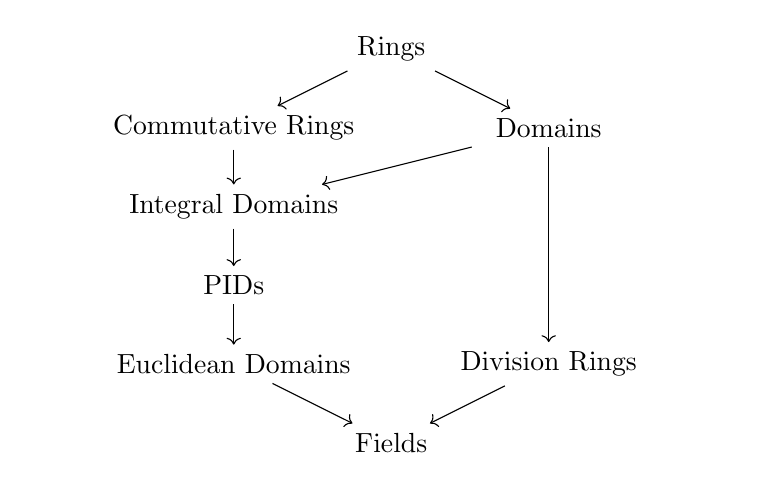
\begin{tikzpicture}[
        node distance=2cm,
        box/.style={
            text width=5cm,
            align=center
        }
    ]
        % Nodes for ring types
        \node[box] (rings) at (0,0) {Rings};
        \node[box] (comm) at (-2,-1) {Commutative Rings};
        \node[box] (domains) at (2,-1) {Domains};
        \node[box] (int) at (-2,-2) {Integral Domains};
        \node[box] (divring) at (2,-4) {Division Rings};
        \node[box] (pid) at (-2,-3) {PIDs};
        \node[box] (euc) at (-2,-4) {Euclidean Domains};
        \node[box] (fields) at (0,-5) {Fields};
        
        % Left path arrows
        \draw[->] (rings) -- (comm);
        \draw[->] (comm) -- (int);
        \draw[->] (int) -- (pid);
        \draw[->] (pid) -- (euc);
        \draw[->] (euc) -- (fields);
        \draw[->] (divring) -- (fields);
        
        % Right path arrows
        \draw[->] (rings) -- (domains);
        \draw[->] (domains) -- (int);
        \draw[->] (domains) -- (divring);
    \end{tikzpicture}
    \caption{Basic hierarchy of rings.} 
    \label{fig:ring_hierarchy}
  \end{figure} 

  \begin{example}[Integers, Rationals, Reals, Complexes]
    The fields $\mathbb{Z}, \mathbb{Q}$, $\mathbb{R}$, and $\mathbb{C}$ are rings with:
    \begin{enumerate}
      \item Sets: 
        \begin{itemize}
          \item $\mathbb{Q}$: rational numbers $\{\frac{a}{b} : a,b \in \mathbb{Z}, b \neq 0\}$
          \item $\mathbb{R}$: real numbers
          \item $\mathbb{C}$: complex numbers $\{a + bi : a,b \in \mathbb{R}\}$
        \end{itemize}
      \item Standard addition and multiplication
      \item Additive identity 0
      \item Multiplicative identity 1
    \end{enumerate}
    These form commutative rings with unity where every non-zero element has a multiplicative inverse.
  \end{example}

  \begin{example}[Continuous Functions]
    The set of all continuous functions $f: \mathbb{R} \rightarrow \mathbb{R}$ is a ring under point-wise addition and multiplication. 
  \end{example}

  \begin{example}[Matrices]
    The ring $M_n(R)$ of $n \times n$ matrices over a ring $R$ consists of:
    \begin{enumerate}
      \item $n \times n$ arrays of elements from $R$
      \item Matrix addition (entry-wise):
      \begin{equation}
        (A + B)_{ij} = A_{ij} + B_{ij}
      \end{equation}
      \item Matrix multiplication:
      \begin{equation}
        (AB)_{ij} = \sum_{k=1}^n A_{ik}B_{kj}
      \end{equation}
      \item Zero matrix as additive identity
      \item Identity matrix $I_n$ as multiplicative identity
    \end{enumerate}
    This forms a non-commutative ring for $n > 1$, even when $R$ is commutative.
  \end{example}

  \begin{example}[Power Set]
    Given a set $X$, let $2^X$ be its power set, that is the set of all subsets of $X$. Then, $2^X$ is a commutative associative ring with respect to the operations of symmetric difference (i.e. the set of elements which is in exactly one of the sets) 
    \begin{equation}
      M \bigtriangleup N \equiv (M \setminus N) \cup (N \setminus M)
    \end{equation}
    and intersection $\cap$, taken for addition an multiplication, respectively. We will not prove all of the axioms of the ring, but we can state some important facts about this structure. The additive identity is $\emptyset$ and the multiplicative identity is $X$. Finally, it is clear that 
    \begin{align*}
      & M \bigtriangleup N \equiv (M \setminus N) \cup (N \setminus M) \equiv N \bigtriangleup M \\
      & M \cap N = N \cap M \\
      & M \cap N \cap P = (M \cap N) \cap P = M \cap (N \cap P)
    \end{align*}
  \end{example}

\subsection{Ring Homomorphisms and Characteristics}

  So far, we have talked about many properties of rings but have not thoroughly gone over their classification. This is what we will do in this section, just like how we have classified groups. It turns out that classifying rings is significantly harder to do so, so we will talk about some low-order finite rings and provide some examples of isomorphisms between more complex rings. Recall that in point set topology, given a topological space $(X, \mathscr{T})$ and its quotient space, if we can construct a map from $X$ to a cleverly chosen space $Z$ that agrees with the quotient, then this induces a homeomorphism $X \cong Z$. 

  \begin{definition}[Ring Homomorphism, Isomorphism]
    A \textbf{ring homomorphism} $f: R \rightarrow S$ is a function that satisfies for all $a, b \in R$
    \begin{enumerate}
      \item $f(a + b) = f(a) + f(b)$
      \item $f(ab) = f(a) f(b)$ 
      \item $f(1_R) = 1_S$
    \end{enumerate}
    for all $a, b \in R$.\footnote{Note that the first is equivalent to it being a group homomorphism between $(R, +)$ and $(S, +)$. The second property may look like it is a group homomorphism between $(R, \times)$ and $(S, \times)$, but remember that neither are groups and it just states that closure distributes. Combined with the fact that the multiplicative identity matches, $f$ is really a homomorphism of \textit{monoids}. } If $f$ is a bijective ring homomorphism, it is called a \textbf{ring isomorphism}. 
  \end{definition} 

  \begin{definition}[Kernel]
    The \textbf{kernel} of a ring homomorphism $f: R \rightarrow S$ is the preimage of $0 \in S$.\footnote{Note that this is the additive identity, not the multiplicative identity. We must specify which identity, unlike a group which has just one identity.}
  \end{definition}

  \begin{lemma}[Properties of Ring Homomorphisms]
    It immediately follows that if $f: R \rightarrow S$ is a ring homomorphism, then 
    \begin{enumerate}
      \item $f(0) = 0$ 
      \item $\Im(f)$ is a subring of $S$. 
      \item A ring homomorphism is injective if and only if $\ker{f} = \langle 0 \rangle $.  
    \end{enumerate}
    Furthermore, if $f$ is a ring isomorphism, then 
    \begin{enumerate}
      \item $f^{-1}$ is a ring isomorphism. 
    \end{enumerate}
  \end{lemma}

  \begin{theorem}[Compositions of Ring Homomorphisms]
    Compositions of ring homomorphisms are ring homomorphisms. 
  \end{theorem} 

\subsection{Commutative Rings} 

  Note that for commutative rings, distinguishing left and right divisors are meaningless, and so we can talk about just \textit{divisors}. 

  \begin{lemma}[Left=Right Divisors]
    In a commutative ring $R$, $a$ is a left divisor of $b$ iff $a$ is a right divisor of $b$. In this case, we just say that $a$ is a \textbf{divisor} of $b$, written $a | b$. 
  \end{lemma}
  \begin{proof}
    $a$ is a right divisor of $b \iff \exists x (xa = b) \iff \exists x (ax = b) \iff a$ is a left divisor. 
  \end{proof} 

  \begin{definition}[Prime and Compositive Elements]
    In a commutative ring $R$, an element $p \in R$ is said to be \textbf{prime} if it is not $0$, not a unit, and has only divisors $1$ and $p$. 
  \end{definition}

  \begin{lemma}[Euclid]
    If $p$ is prime, then $p|ab \implies p|a$ or $p|b$.  
  \end{lemma}

  \begin{lemma} 
    Let $R$ be a commutative ring and $a, b, d \in R$. If $d|a$ and $d|b$, then $d | (ma + nb)$ for any $m, n \in R$. 
  \end{lemma} 

  \begin{definition}[Greatest Common Divisor]
    The \textbf{greatest common divisor} of elements $a$ and $b$, denoted $\gcd(a, b)$ of an commutative ring $R$ is a common divisor of $a$ and $b$ divisible by all their common divisors. That is, it is the element $d \in R$ satisfying 
    \begin{enumerate}
      \item $d \mid a$ and $d \mid b$ 
      \item if $k \mid a$ and $k \mid b$, then $k \mid d$. 
    \end{enumerate}
    If $\mathrm{gcd}(a, b) = 1$, then $a$ and $b$ are said to be \textbf{relatively prime}. 
  \end{definition} 

  Note that in an arbitrary commutative ring, the gcd of two elements always exists since we can at least identify $1$, but there may not be a \textit{unique} gcd. 

\subsection{Domains}

  We can see that domains behave similarly to the integers, but with the missing property that $\times$ is commutative. This motivates the following definition of an integral domain, which can be seen as a generalization of the integers. 

  \begin{definition}[Domain]
    A ring $R$ with no zero divisors for every element is called a \textbf{domain}. An \textbf{integral domain} is a commutative domain $R$.\footnote{Almost always, we work with integral domains so we will default to this.} 
  \end{definition} 

  \begin{example}[Domains vs Integral Domains]
    We show some examples of integral domains. 
    \begin{enumerate}
      \item The ring $\mathbb{Z}$ of integers. 
      \item The field $\mathbb{R}$. 
      \item The ring $\mathbb{Z}[x]$ of polynomials of one variable with integer coefficients. 
    \end{enumerate}
    We show examples of domains that are not integral domains. 
    \begin{enumerate}
      \item Quaternions $\mathbb{H}$ are not commutative but are a domain. 
    \end{enumerate}
  \end{example} 

  \begin{theorem}[Fields are Integral Domains]
    Every field is an integral domain. 
  \end{theorem}
  \begin{proof}
    
  \end{proof}

  \begin{theorem}[Polynomial Integral Domains]
    Rings of polynomials are an integral domain if the coefficients come from an integral domain. 
  \end{theorem}
  \begin{proof}
    
  \end{proof} 

  Factorization of polynomials over $\mathbb{C}$ into linear factors and polynomials over $\mathbb{R}$ into linear and quadratic factors is similar to the factoring of the integers to prime numbers. In fact, such a factorization exists for polynomials over any field $F$, but their factors can be of any degree. Moreover, there exists no general solution for the factoring of polynomials over any field. 

  \begin{example}
    $\mathbb{Z}$ and $F[x]$ over field $F$ are integral domains. Any field $F$ is also an integral domain. 
  \end{example}

  \begin{example}
    The quotient ring $\mathbb{Z}_n$ is not an integral domain when $n$ is composite. 
  \end{example}

  \begin{example}
    A product of two nonzero commutative rings with unity $R \times S$ is not an integral domain since $(1,0) \cdot (0, 1) = (0, 0) \in R \times S$. 
  \end{example}

  \begin{example}
    The ring of $n \times n$ matrices over any nonzero ring when $ n \geq 2$ is not an integral domain. Given matrices $A, B$, if the image of $B$ is in the kernel of $A$, then $A B = 0$.
  \end{example}

  \begin{example}
    The ring of continuous functions on the interval is not an integral domain. To see why, notice that given the piecewise functions 
    \begin{equation}
      f (x) = \begin{cases}
      1 - 2x & x \in [0, \frac{1}{2}] \\
      0 & x \in [\frac{1}{2}, 1] 
      \end{cases}, \; \;\;g (x) = \begin{cases}
      0 & x \in [0, \frac{1}{2}] \\
      2x - 1 & x \in [\frac{1}{2}, 1] 
      \end{cases}
    \end{equation}
    $f, g \neq 0$, but $f g = g f = 0$. 
  \end{example}

  \begin{theorem}
    An integral domain is a ring that is isomorphic to a subring of a field. 
  \end{theorem}

  \begin{theorem}
    The characteristic of an integral domain is either $0$ or a prime number. 
  \end{theorem}

  \begin{definition}[Regular Elements]
     An element $r$ of a ring $R$ is \textbf{regular} if the mapping 
     \begin{equation}
       \rho: R \longrightarrow R, \qquad x \mapsto x r
     \end{equation}
    is injective for all $x \in R$. 
  \end{definition}

  \begin{theorem}
    An integral domain is a commutative associative ring where every element is regular. 
  \end{theorem} 

  While we have shown that gcd's exist in commutative rings, we can say a bit more when working in Euclidean domains. 

  \begin{definition}[Associate Elements]
    Elements $a$ and $b$ are \textbf{associated}, denoted $a \sim b$ if either of the following equivalent conditions holds
    \begin{enumerate}
        \item $a | b \text{ and } b | a$
        \item $a = c b, \text{ where } c$ is invertible
    \end{enumerate}
    The two conditions are equivalent because $c$ and $c^{-1}$ are both in $A$. 
  \end{definition} 

  \begin{theorem}[GCD's in a Euclidean Domain]
    Any two distinct gcd's of $a, b$ in a Euclidean domain must be associate elements. 
  \end{theorem}

\subsection{Ideals}

  Now assuming that $R$ and $S$ are commutative rings, let's consider a special sort of subset of a commutative ring. Consider the kernel of the ring homomorphism. We can see that if $a, b \in \ker(f)$, then $f(a + b) = f(a) + f(b) = 0 + 0 = 0$, and so $\ker(f)$ is closed under addition. Furthermore, $a \in \ker(f)$ and \textit{any} $b \in R$ gives $f(ab) = f(a) f(b) = 0 f(b) = 0$, and so multiplying any element in the kernel by an arbitrary element in the rings keeps it in the kernel. We would like to generalize these properties into an \textit{ideal}. 

  \begin{definition}[Ideals]
    For a commutative ring $(R,+, \times)$, a \textbf{two-sided ideal}---or \textbf{ideal}---is a subset $I \subset R$ satisfying 
    \begin{enumerate}
      \item $a, b \in I \implies a + b \in I$. 
      \item $a \in I, r \in R \implies ra = ar \in I$.
    \end{enumerate}
    If $R$ is not necessarily commutative, then we $ra \neq ar$ in general, so we may distinguish between left and right ideals. 
  \end{definition}

  Let's try to elaborate more on this interpretation by introducing immediate consequences. 

  \begin{lemma}[Ideals are Groups Under $+$]
    Given a commutative ring $R$ and ideal $I \subset R$, $(I, +)$ is an abelian group. 
  \end{lemma}

  Therefore, we can see that it is an abelian group under $+$ and closed under $\times$. However, it is not guaranteed to have a multiplicative identity, which is why we can interpret $I$ as a ring without a multiplicative identity, also known as a \textit{rung}. 

  \begin{example}[Multiples of Elements Are an Ideal]
    We give 2 ideals: 
    \begin{enumerate}
      \item The set of even integers $2 \mathbb{Z}$ is an ideal in the ring $\mathbb{Z}$, since the sum of any even integers is even and the product of any even integer with an integer is an even integer. However, the odd integers do not form an ideal. 
      \item The set of all polynomials with real coefficients which are divisible by the polynomial $x^2 + 1$ is an ideal in the ring of all polynomials. 
    \end{enumerate}
  \end{example}

  Given these two examples, we can think of an ideal consisting of all multiples of a specific element $a$ that \textit{generates} the ideal. 

  \begin{definition}[Generators of Ideals]
    Given a commutative ring $R$, the \textbf{ideal generated by $a \in R$} is denoted 
    \begin{equation}
      \langle a \rangle \coloneqq \{r a \mid r \in R\}
    \end{equation}
    and more generally, we may have multiple generating elements. 
    \begin{equation}
      \langle a_1, \ldots, a_n \rangle \coloneqq \{ r_1 a_1 + \ldots r_n a_n \mid r_1, \ldots, r_n \in R \}
    \end{equation}
  \end{definition}

  Therefore, the ideals considered above can be written $\langle 2 \rangle \subset \mathbb{Z}$ and $\langle x - 2 \rangle \subset \mathbb{Q}[x]$. However, it may be the case that two elements generate the same ideal in a non-Euclidean domain, but constructing such an example is a bit challenging.   

  \begin{example}[Matrix with Last Row of Zeros]
    The set of all $n \times n$ matrices whose last row is zero forms a right ideal in the ring of all $n \times n$ matrices. However, it is not a left ideal.

    The set of all $n\times n$ matrices whose last column is zero is a left ideal, but not a right ideal. 
  \end{example}

  \begin{theorem}[Ideals of Fields]
    The only ideals that exist in a field $\mathbb{F}$ is $\{0\}$ and $\mathbb{F}$ itself. 
  \end{theorem}
  \begin{proof}
    Given a nonzero element $x \in \mathbb{F}$, every element of $\mathbb{F}$ can be expressed in the form of $a x$ or $x a$ for some $a \in \mathbb{F}$. 
  \end{proof}

\subsection{Quotient Rings}

  What is nice about ideals is that they induce an equivalence relation defined on a ring, which reminds you of working in modulos on the integers. 

  \begin{theorem}[Equivalence Relation Induced by an Ideal]
    Given a commutative ring $R$ and an ideal $I \subset R$, we say that two elements $a, b \in R$ are equivalent $\pmod{I}$, written $a \equiv b \pmod{I}$ iff $a - b \in I$. We claim two things: 
    \begin{enumerate}
      \item $\equiv$ is indeed an equivalence relation. 
      \item Given that $a \equiv a^\prime \pmod{I}$ and $b = b^\prime \pmod{I}$, 
        \begin{equation}
          a + b \equiv a^\prime + b^\prime \pmod{I}, \qquad ab \equiv a^\prime b^\prime \pmod{I}
        \end{equation}
    \end{enumerate}
  \end{theorem}
  \begin{proof}
    We first prove that $\equiv$ is indeed an equivalence relation. 
    \begin{enumerate}
      \item \textit{Reflexive}. $a \equiv a \pmod{I}$ is trivial since $a - a = 0 \in I$. 
      \item \textit{Transitive}. If $a \equiv b$. 
    \end{enumerate}
  \end{proof} 

  This quotient space maintains a lot of nice properties of the algebraic operations, and so we can form a new ring structure with this quotient space.  

  \begin{definition}[Quotient Rings, Rings of Residue Class]
    The quotient space $R/I$ induced by the mapping $a \mapsto [a]$ is indeed a commutative ring, called the \textbf{quotient ring}, with addition and multiplication defined 
    \begin{equation}
      [a] + [b] \coloneqq [a + b], \qquad [ab] \coloneqq [a] \, [b]
    \end{equation}
  \end{definition}
  \begin{proof}
    Note that the properties of the operation in $\frac{M}{R}$ inherits all the properties of the addition operation on $M$ that are expressed in the form of identities and inverses, along with the existence of the zero identity. 
    \begin{align*}
      0 \in M & \implies [0] \text{ is the additive identity in } \frac{M}{R} \\
      a + (-a) = 0 & \implies [a] + [-a] = [0] \\
      1 \in M & \implies [1] \text{ is the multiplicative identity in } \frac{M}{R}
    \end{align*}
  \end{proof} 

  \begin{example}[Quotient Rings of Integers]
    The quotient set $\mathbb{Z}/\langle n \rangle$ by the relation of congruence modulo $n$ is denoted $\mathbb{Z}_{n}$. 
    \begin{equation}
      \mathbb{Z}_{n} = \{ [0]_{n}, [1]_{n}, \ldots, [n-1]_{n} \}
    \end{equation}
    We list some quotient rings of the integers.  
    \begin{enumerate}
      \item In $\mathbb{Z}_{5} = \mathbb{Z}/\langle 5 \rangle$, the elements $[2]$ and $[3]$ are multiplicative inverses of each other since $[2] [3] = [6] = [1]$, and $[4]$ is its own inverse since $[4] [4] = [16] = [1]$. The addition and multiplication tables for $\mathbb{Z}_5$ is shown below. 
      \item Consider the ideal $I = \langle 2 \rangle \subset \mathbb{Z}_6$. We have $0 \equiv 2 \equiv 4 \pmod{I}$ and $1 \equiv 3 \equiv 5 \pmod{I}$, and so the quotient ring $\mathbb{Z}_6 / I$ consists of the two equivalence classes $[0]$ and $[1]$. 
    \end{enumerate}
  \end{example}

  \begin{example}[Quotient Rings of Polynomials]
    We list some quotient rings of the integers.  
    \begin{enumerate}
      \item Consider $\mathbb{Q}[x] / \langle x^2 - 2 \rangle$. We can see that any polynomial $f \in \mathbb{Q}[x]$ is equivalent $\pmod{I}$ to a linear polynomial, since $x^2 \equiv 2$. Alternatively we can apply the division algorithm to replace $f(x)$ by its remainder upon division by $x^2 - 2$, and thus in the quotient ring, $[x]$ plays the role of $\sqrt{2}$, which may indicate that $\mathbb{Q}[x] / \langle x^2 - 2 \rangle = \mathbb{Q}[\sqrt{2}]$. 
      \item Consider $\mathbb{Z}_2 [x]/ \langle x^2 + x + 1 \rangle$. As in the previous example, any polynomial in $\mathbb{Z}_2[x]$ is equivalent to a linear polynomial since $x^2 \equiv x + 1 \pmod{I}$. Therefore the elements of the quotient ring are $[0], [1], [x], [x+1]$ with the addition and multiplication tables. 

      \begin{figure}[H]
        \centering
        \begin{subfigure}[b]{0.48\textwidth}
          \centering
          \begin{tabular}{c|cccc}
            $+$ & $0$ & $1$ & $x$ & $x + 1$ \\
            \hline
            $0$ & $0$ & $1$ & $x$ & $x + 1$ \\
            $1$ & $1$ & $0$ & $x + 1$ & $x$ \\
            $x$ & $x$ & $x + 1$ & $0$ & $1$ \\
            $x + 1$ & $x + 1$ & $x$ & $1$ & $0$ \\
          \end{tabular}
          \caption{}
        \end{subfigure}
        \hfill 
        \begin{subfigure}[b]{0.48\textwidth}
          \centering
          \begin{tabular}{c|cccc}
            $\cdot$ & $0$ & $1$ & $x$ & $x + 1$ \\
            \hline
            $0$ & $0$ & $0$ & $0$ & $0$ \\
            $1$ & $0$ & $1$ & $x$ & $x + 1$ \\
            $x$ & $0$ & $x$ & $x + 1$ & $1$ \\
            $x + 1$ & $0$ & $x + 1$ & $1$ & $x$ \\
          \end{tabular}
          \caption{}
        \end{subfigure}
        \label{fig:boolean-algebra-tables}
      \end{figure}
    \end{enumerate}
  \end{example}

  Note that just like how quotient topologies do not preserve topological properties, as shown \hyperref[pst-quotient_trivial]{here} and \hyperref[pst-quotient_hausdorff]{here}, quotient rings inherit some---but not all---algebraic properties. 

  \begin{theorem}[Quotient Inherits Commutativity]
    Let $R$ be a commutative ring and $I \subsetneq R$ be an ideal. Then $R/I$ is a commutative ring. 
  \end{theorem}

  \begin{example}[Quotient Does Not Inherit Integral Domain Property]
    $\mathbb{Z}$ is an integral domain, but $\mathbb{Z}/\langle 6 \rangle$ is not since $[2] \times [3] = [0]$. 
  \end{example}


  The ring $\mathbb{Z}_n$ has all the properties of a field except the property of having inverses for all of its nonzero elements. This leads to the following theorem. 

  \begin{theorem}[Integer Quotient Rings as Finite Fields]
    The ring $\mathbb{Z}_{n}$ is a field if and only if $n$ is a prime number. 
  \end{theorem}
  \begin{proof}
    $(\rightarrow)$ Assume that $n$ is composite $\implies n = k l$ for $k, n \in \mathbb{N} \implies k, n \neq 0$, but 
    \begin{equation}
      [k]_n [l]_n = [k l]_n = [n]_n = 0
    \end{equation}
    meaning that $\mathbb{Z}_n$ contains $0$ divisors and is not a field. The contrapositive of this states $(\rightarrow)$. \\
    $(\leftarrow)$ Given that $n$ is prime, let $[a]_n \neq 0$, i.e. $[a]_n \neq [0]_n, [1]_n$. The set of $n$ elements 
    \begin{equation}
      [0]_n, [a]_n, [2a]_n, ..., [(n-1)a]_n
    \end{equation}
    are all distinct. Indeed, if $[k a]_n = [l a]_n$, then $[(k-l) a]_n = 0 \implies n = (k-l) a \iff n$ is not prime. Since the elements are distinct, exactly one of them must be $[1]_n$, say $[p a]_n \implies$ the inverse $[p]_n$ exists. 
  \end{proof}

  \begin{corollary}[Invertibility in $\mathbb{Z}_n$]
    For any $n$, $[k]_n$ is invertible in the ring $\mathbb{Z}_n$ if and only if $n$ and $k$ are relatively prime. 
  \end{corollary} 

  \begin{theorem}[Wilson's Theorem]
    Let $n$ be a prime number. Then 
    \begin{equation}
      (n-1)! \equiv -1 \pmod{n}
    \end{equation}
  \end{theorem}

\subsection{Homomorphism and Isomorphism Theorems}

  \begin{theorem}[Fundamental Ring Homomorphism Theorem]
    Let $R$ and $S$ be commutative rings, and suppose $f: R \rightarrow S$ be a surjective ring homomorphism. Then this induces a ring isomorphism
    \begin{equation}
      R /\ker{f} \simeq S
    \end{equation} 
    satisfying $\phi = \bar{\phi} \circ \pi$. 

    \begin{figure}[H]
      \centering 
      \begin{tikzcd}
        R \arrow[r, "\phi"] \arrow[d, "\pi"] & S \\
        R/\ker(\phi) \arrow[ru, "\bar{\phi}"] &  
      \end{tikzcd}
      \caption{The theorem states that the following diagram commutes. } 
      \label{fig:fund_ring_homo_theorem}
    \end{figure}
  \end{theorem}
  \begin{proof}
    
  \end{proof} 

\subsection{Unique Factorization Domain}

\subsection{Principal Ideal Domains}

  A good intuition to have about ideals is that they are the set of multiples of a certain element. However, this may not be true for ideals in general, but if this intuition is true, then we call this a \textit{principal ideal}. 

  \begin{definition}[Principal Ideals]
    Given commutative ring $R$ and $I \subset R$, if $I = \langle a \rangle$ for some $a \in R$---i.e. it is generated by a single element---$I$ is called a \textbf{principal ideal}. 
  \end{definition}

  \begin{definition}[Principal Ideal Domain]
    A \textbf{principal ideal domain}, also called a \textbf{PID}, is an integral domain in which every ideal is principal. 
  \end{definition}

  More generally, a \textbf{principal ideal ring} is a nonzero commutative ring in which every ideal is principal (i.e. can be generated by a single element). The distinction is that a principal ideal ring may have zero divisors whereas a principal ideal domain cannot. Principal ideal domains are thus mathematical objects that behave somewhat like the integers. That is, 
  \begin{enumerate}
    \item Any element of a PID has a unique decomposition into prime elements. 
    \item Any two elements of a PID have a greatest common divisor. 
    \item If $x$ and $y$ are elements of a PID without common divisors, then every element of the PID can be written in the form 
      \begin{equation}
        a x + b y
      \end{equation}
  \end{enumerate}

  We now introduce some examples of PIDs, which are not as trivial and should be introduced as theorems. 

  \begin{theorem}[Integers and Polynomials over Fields are PIDs]
    The following are all examples of principal ideal domains. 
    \begin{enumerate}
      \item Any field $\mathbb{F}$. 
      \item The ring of integers $\mathbb{Z}$. 
      \item $\mathbb{F}[x]$, rings of polynomials in one variable with coefficients in a field $\mathbb{F}$. 
    \end{enumerate}
  \end{theorem}
  \begin{proof}
    Listed. 
    \begin{enumerate}
      \item It is quite easy to see that a field $\mathbb{F}$ is a PID since the only two possible ideals are $\{0\}$ and $\mathbb{F}$, both of which are principal. 
      \item If $I \subset \mathbb{Z}$ is an ideal, then if $I = \langle 0 \rangle$, then we're done. Otherwise, let $a \in I$ be the smallest positive integer in $I$. It is clear that $\langle a \rangle \subset I$. Now given an element $b \in I$, by the Euclidean algorithm we have $b = aq + r$ with $r < a$. Since $a, b \in I$, it follows that $r \in I$. But since $0 \leq r < a$ and $a$ is the smallest positive integer, $r = 0$, and so $b = aq \implies b \in \langle a \rangle$. 
      \item The ring of polynomials $\mathbb{F}[x]$ is a PID since we can imagine a minimal polynomial $p$ in each ideal $I$. Every element in $I$ must be divisible by $p$, which means that the entire ideal $I$ can be generated by the minimal polynomial $p$, making $I$ principal.  
    \end{enumerate}
  \end{proof}

  \begin{corollary}[Ideals Generated by Primes]
    If $I \subsetneq \mathbb{Z}$ and a prime number $p \in I$, then $I = \langle p \rangle$. If $I \subset F[x]$ is an ideal and irreducible $f(x) \in I$, then $I = \langle f(x) \rangle$. 
  \end{corollary}
  \begin{proof}
    Listed. 
    \begin{enumerate}
      \item Since $\mathbb{Z}$ is a PID, $I = \langle a \rangle$ for some nonzero $a \in \mathbb{Z}$. We can assume $a$ is positive, and if $a = 1$, then $I = \mathbb{Z}$, which contradicts the $I$ is a proper subset. So $a \geq 2$. Now because $p \in I$, $p = ra$ for some $r \in \mathbb{Z}$, but since $p$ is prime, $r = 1, a = p$. 

      \item Since $F[x]$ is a PID and $I = \langle g(x) \rangle$ for some $g(x) \in F[x]$, let us take $f(x) \in I$. Then it must be true that $f(x) = g(x) h(x)$ for some $h(x) \in R$. However, This means that $\deg(g)$ or $\deg(h)$ must be $0$ since $f$ is irreducible. But if $g(x)$ was a constant, then $I = R$, so $g(x) = f(x)$. 
    \end{enumerate}
  \end{proof}

  \begin{corollary}[Kernel of Evaluation Homomorphism is Generated by Irreducible Factor]
    Suppose $f(x) \in F[x]$ is irreducible in $F[x]$, and $K \supset F$ is a field containing a root $\alpha$ of $f(x)$. Then the ideal of all polynomials in $F[x]$ vanishing at $\alpha$ is generated by $f(x)$. That is, given the evaluation homomorphism 
    \begin{equation}
      \ev_\alpha: F[x] \rightarrow K
    \end{equation}
    we claim $\ker(\ev_\alpha) = \langle f(x) \rangle$. 
  \end{corollary}
  \begin{proof}
    This is an immediate consequence of the previous corollary. 
  \end{proof}

  The great thing about PIDs is that they unlock a lot of the familiar properties that we see in the integers. In fact, pretty much everything holds except for the existence of Euclidean algorithm for factorization. 

  \begin{theorem}[Greatest Common Divisor]
    Given $a, b \in R$ a PID, $\gcd(a, b)$ is unique. 
  \end{theorem}

  \begin{theorem}[Unique Factorization Theorem]
    Every element $x \in R$ of a PID can be uniquely factored (up to permutations and units) into irreducible elements in $R$. 
  \end{theorem}

  Bezout's does not hold in integral domains in general. 

  \begin{theorem}[Bezout's Theorem]
    Given that one divides (with remainder) polynomial $f$ by $g = x - c$, let the remainder be $r \in F$. That is, 
    \begin{equation}
      f(x) = (x-c) q(x) + r, \; r \in F
    \end{equation}
    This implies that the remainder equals the value of $f$ at point $c$. That is, 
    \begin{equation}
      f(c) = r
    \end{equation}
    Note that a corollary of this is the single factorization theorem, but the single factorization holds for commutative rings in general. 
  \end{theorem} 

\subsection{Euclidean Domains}

  \begin{definition}[Euclidean Domain]
    Let $R$ be an integral domain which is not a field. $R$ is \textbf{Euclidean domain} if 
    \begin{enumerate}
      \item there exists a \textit{norm} $|\cdot|: R \setminus \mathbb{R}_0^+$, and  
      \item there exists a well-defined function, called \textbf{Euclidean division} $\mathcal{D}: R \times R \rightarrow R \times R$ that is defined 
      \begin{equation}
        \mathcal{D}(a, b) = (q, r) \text{ where } a = bq + r \text{ and } 0 \leq r < |b|
      \end{equation}
    \end{enumerate}
  \end{definition}

  The two prime examples are the integers and polynomials. 

  \begin{example}[Integers]
    $\mathbb{Z}$ is a Euclidean domain with Euclidean division, also called long division, defined 

    \begin{center}
      \intlongdivision{521}{13}
    \end{center}
  \end{example}

  \begin{theorem}[Polynomials are Euclidean Domains]
    Let $f(x), g(x) \in F[x]$ and $g(x) \neq 0$. Then, there exists polynomials $q(x), r(x)$ such that 
    \begin{equation}
      f(x) = q(x) g(x) + r(x), \qquad 0 \leq \deg(r) < \deg(g)
    \end{equation}
    where $\deg$ is the norm.
  \end{theorem}

  \begin{example}[Gaussian Integers]
    The subring of $\mathbb{C}$, defined
    \begin{equation}
      \mathbb{Z}[i] \equiv \{ a + b i \mid a, b \in \mathbb{Z} \}
    \end{equation}
    is a Euclidean integral domain with respect to the norm 
    \begin{equation}
      N(c) \equiv a^2 + b^2
    \end{equation}
    since $N(c d) = N(c) N(d)$ and the invertible elements of $\mathbb{Z}[i]$ are $\pm 1, \pm i$. 
  \end{example}

  \begin{example}[Dyadic Rationals]
    The ring of rational numbers of the form $2^{-n} m, \; n \in \mathbb{Z}_+, m \in \mathbb{Z}$, is a Euclidean domain. To define the norm, we can first assume that $m$ can be prime factorized into the form 
    \begin{equation}
      m = \pm \prod_{i} p_{i}^{k_i}, \; p \text{ prime}
    \end{equation}
    and the norm is defined 
    \begin{equation}
      N(\frac{m}{2^n}) \equiv 1 + \sum_i k_i
    \end{equation}
    We must further show that division with remainder is possible, but we will not show it here. 
  \end{example}

  \begin{theorem}[Chinese Remainder Theorem]
    
  \end{theorem}

\subsection{Division Rings}

  \begin{definition}[Division Ring]
    A \textbf{division ring}, also called a \textbf{skew field}, is an associative ring where every nonzero element is invertible with respect to $\times$.\footnote{Division rings differ from fields in that multiplication is not required to be commutative. }
  \end{definition}

  Let's establish the hierarchy. 

  \begin{lemma}[Division Rings are Domains]
    Every division ring $R$ is automatically a domain. 
  \end{lemma}
  \begin{proof}
    Every nonzero element is invertible. 
  \end{proof}

  \begin{example}[Invertible Matrices are a Division Ring]
    At first, a division ring may not seem different from a field. However, a classic example is the ring of invertible matrices, which is not necessarily commutative, but is a ring in which "division" can be done by right and left multiplication of a matrix inverse. 
    \begin{equation}
      a a^{-1} = a^{-1} a = I
    \end{equation}
    This implies that every element in the division ring commutes with the identity, but again commutativity does not necessarily hold for arbitrary elements $a, b$. 
  \end{example} 

\subsection{Fields}

  Our final structure is field, which are usually pretty tame compared to groups and rings. 

  \begin{definition}[Field]
    A \textbf{field} $(F, +, \times)$ is a commutative, associative ring where every nonzero element is a unit. 
  \end{definition}

  \begin{lemma}[Properties of Addition]
    The properties of addition hold in a field. 
    \begin{enumerate}
      \item If $x + y = x + z$, then $y = z$. 
      \item If $x + y = x$, then $y = 0$. 
      \item If $x + y = 0$, then $y = -x$. 
      \item $(-(-x)) = x$. 
    \end{enumerate}
  \end{lemma}
  \begin{proof}
    For the first, we have 
    \begin{align}
      x + y = x + z & \implies -x + (x + y) = -x + (x + z) && \tag{addition is a function} \\
                    & \implies (-x + x) + y = (-x + x) + z && \tag{$+$ is associative} \\
                    & \implies 0 + y = 0 + z && \tag{definition of additive inverse} \\
                    & \implies y = z && \tag{definition of identity}
    \end{align} 
    For the second, we can set $z = 0$ and apply the first property. For the third, we have 
    \begin{align}
      x + y = 0 & \implies -x + (x + y) = -x + 0 && \tag{addition is a function} \\
                & \implies (-x + x) + y = -x + 0 && \tag{$+$ is associative} \\
                & \implies 0 + y = -x + 0 && \tag{definition of additive inverse} \\
                & \implies y = -x && \tag{definition of identity}
    \end{align}
    For the fourth, we simply follow that if $y$ is an inverse of $z$, then $z$ is an inverse of $y$. Therefore, $-x$ being an inverse of $x$ implies that $x$ is an inverse of $-x$. $-(-x)$ must also be an inverse of $-x$. Since inverses are unique\footnote{This is proved in algebra.}, $x = -(-x)$. 
  \end{proof}

  \begin{lemma}[Properties of Multiplication]
    The properties of multiplication hold in a field. 
    \begin{enumerate}
      \item If $x \neq 0$ and $xy = xz$, then $y = z$. 
      \item If $x \neq 0$ and $xy = x$, then $y = 1$. 
      \item If $x \neq 0$ and $xy = 1$, then $y = x^{-1}$. 
      \item If $x \neq 0$, then $(x^{-1})^{-1} = x$. 
    \end{enumerate}
  \end{lemma}
  \begin{proof}
    The proof is almost identical to the first. Since $x \neq 0$, we can always assume that $x^{-1}$ exists. For the first, we have
    \begin{align}
      x y = x z & \implies x^{-1} (x y) = x^{-1} (x z) && \tag{multiplication is a function} \\
                & \implies (x^{-1} x) y = (x^{-1} x) z && \tag{$\times$ is associative} \\
                & \implies 1 y = 1 z && \tag{definition of multiplicative inverse} \\  
                & \implies y = z && \tag{definition of identity}
    \end{align}
    For the second, we can set $z = 1$ and apply the first property. For the third, we have 
    \begin{align}
      xy = 1 & \implies x^{-1} (x y) = x^{-1} 1 && \tag{multiplication is a function} \\
             & \implies (x^{-1} x) y = x^{-1} 1 && \tag{$\times$ is associative} \\
             & \implies 1 y = x^{-1} 1 && \tag{definition of multiplicative inverse} \\
             & \implies y = x^{-1} && \tag{definition of identity}
    \end{align}
    For the fourth, we simply see that $x^{-1}$ is a multiplicative inverse of both $x$ and $(x^{-1})^{-1}$ in the group $(\mathbb{F} \setminus \{0\}, \times)$, and since inverses are unique, they must be equal. 
  \end{proof}

  \begin{lemma}[Properties of Distribution]
    For any $x, y, z \in \mathbb{F}$, the field axioms satisfy 
    \begin{enumerate}
      \item $0 \cdot x = 0$.
      \item If $x \neq 0$ and $y \neq 0$, then $x y \neq 0$.
      \item $-1 \cdot x = -x$. 
      \item $(-x) y = - (xy) = x (-y)$. 
      \item $(-x) (-y) = xy$. 
    \end{enumerate}
  \end{lemma} 
  \begin{proof}
    For the first, note that 
    \begin{align}
      0 x & = (0 + 0) \cdot x = 0 x + 0x 
    \end{align}
    and subtracting $0x$ from both sides gives $0 = 0x$. For the second, we can claim that $xy \neq 0$ equivalently claiming that it will have an identity. Since $x, y \neq 0$, their inverses exists, and we claim that $(xy)^{-1} = y^{-1} x^{-1}$ is an inverse. We can see that by associativity, 
    \begin{equation}
      (y^{-1} x^{-1}) (xy) = y^{-1} (x^{-1} x) y = y^{-1} y = 1
    \end{equation} 
    For the third, we see that 
    \begin{equation}
      0 = 0 \cdot x = (1 + (-1)) \cdot x = 1 \cdot x + (-1) \cdot x = x + (-1) \cdot x 
    \end{equation}
    which implies that $-1 \cdot x$ is the additive inverse. The fourth follows immediately from the third by the associative property. For the fifth we can see that 
    \begin{align}
      (-x) (-y) & = (-1) x (-1) y && \tag{property 3} \\
                & = (-1) (-1) x y && \tag{$\times$ is commutative} \\
                & = -1 \cdot (-xy) && \tag{property 3} \\
                & = -(-xy) && \tag{property 3} \\
                & = xy && \tag{addition property 4}
    \end{align}
  \end{proof}


  \begin{theorem}
    Every field is a Euclidean domain. 
  \end{theorem}
  \begin{proof}
    Given $x, y \in \mathbb{F}$, assume $x y = 0$ with $x \neq 0$. Since $x$ is invertible,
    \begin{equation}
      0 = x^{-1} 0 = x^{-1} (x y) = y
    \end{equation}
    Now assuming that $y \neq 0$, since $y$ is invertible, 
    \begin{equation}
      0 = 0 y^{-1} = (x y) y^{-1} = x
    \end{equation}
  \end{proof}

  Let's give a few examples of fields. 

  \begin{theorem}[Wedderburn's little theorem]
    Every finite Euclidean domain is a field. 
  \end{theorem} 

  \begin{example}[Finite Fields]
    $\mathbb{Z}_p$ with $p$ prime is a field. 
  \end{example}




\section{Polynomial Rings} 

  In ring theory, the idea of \textit{adjoining} an existing ring $R$ with an arbitrary element $x$ will appear frequently. That is, given a ring $R$ and some $x$, can we try and construct a new ring $S$, denoted $R[x]$ that is the minimal ring containing both $R$ and $x$? What kind of elements would be in $R[x]$? 
  \begin{enumerate}
    \item Since $R \subset R[x]$, it must be the case that for $a \in R$, $a \in R[x]$. 
    \item Since $x \in R[x]$, it must be the case that $a x \in R[x]$ for all $a \in R$. 
    \item $x \times x = x^2 \in R[x]$, so it must be the case that $a x^2 \in R[x]$ 
    \item In general, for any $n \in \mathbb{N}$, $x^n \in R[x]$, so it must be the case that $a x^n \in R[x]$. 
  \end{enumerate}
  If we add these terms up, we have elements of the general form 
  \begin{equation}
    a_n x^n + a_{n-1} x^{n-1} + \ldots + a_1 x + a_0 
  \end{equation}
  This is what we refer to as a polynomial, and it indeed does have a ring structure. More generally, given a set of elements $S = \{x_1, \ldots, x_n\}$, $R[S]$ can be defined accordingly. Now let's formally define them. 

  \begin{definition}[Polynomial Ring]
    Given ring $R$ and a set of \textbf{indeterminates} $S = \{x_1, \ldots, x_n\}$, the \textbf{ring of polynomials} $R[S] = R[x_1, \ldots, x_n]$ is defined in the equivalent ways. 
    \begin{enumerate}
      \item It is the minimal ring containing $R$ as a subring and $x$. 
      \item It is the ring of formal expressions of the form 
      \begin{equation}
        f(x_1, \ldots, x_n) = \sum_{0 \leq k_i \leq n} a_{k_1 \ldots k_n} x_1^{k_1} x_2^{k_2} \ldots x_n^{k_n}, \quad a_i \in R
      \end{equation}
      which for univariate polynomials simplifies to 
      \begin{equation}
        f(x) = a_nx^n + a_{n-1}x^{n-1} + \dots + a_1 x + a_0, \quad a_i \in R
      \end{equation}
    \end{enumerate}
    From both definitions is becomes clear through the ring properties that 
    \begin{enumerate}
      \item Addition is defined component-wise: $a x^i + b x^i = (a + b) x^i$. 
      \item Multiplication is defined component-wise: $x^i x^j = x^{i + j}$. 
      \item Additive and multiplicative identities is $0$ and $1$. 
    \end{enumerate}
  \end{definition}

  Note that $x$ is just a formal symbol, whose powers $x^i$ are just placeholders for the corresponding coefficients $a_i$ so that the given formal expression is a way to encode the finitary sequence. $(a_0, a_1, a_2, ..., a_n)$. Two polynomials are equal if and only if the sequences of their corresponding coefficients are equal. Also note that unlike a function, which we write as $f$, for a polynomial we should write the indeterminate $f(x)$. We can however interpret $f(x)$ as a function as well (which may not be unique), and doing so allows us to determine special properties of $f(x) \in R[x]$. Before we move on, let's get some terms out of the way. 

  \begin{definition}[Some Terms for Polynomials]
    Given a univariate polynomial $f(x) \in R[x]$. 
    \begin{enumerate} 
      \item The \textbf{leading coefficient} is the last nonzero coefficient  
      \item The \textbf{degree} of $f$---denoted $\deg f$---is the index of the leading coefficient.
      \item A \textbf{monomial} is a polynomial of a single term $a_j x^j$. 
      \item A \textbf{linear} polynomial is a polynomial of degree 1. 
      \item A \textbf{quadratic} polynomial is a polynomial of degree 2. 
      \item A \textbf{cubic} polynomial is a polynomial of degree 3. 
    \end{enumerate}
  \end{definition}

  We need to be very careful about the properties that hold for polynomials, as they may not be intuitive. For example, for certain finite fields (which are rings), some formally different polynomials may be indistinguishable in terms of mappings.\footnote{$x$ and $x^2$ are equivalent in  $\mathbb{Z}_2 [x]$. } Second, a polynomial may have more roots than its degree. Therefore, we will work in different rings $R$ and provide conditions where our intuition is true in $R[x]$. It is clear that if you have two polynomials of degree $n$ and $m$, their sum may be degree $k < n, m$. This is not always true for multiplication. 

  \begin{example}[Product of Two Linear Polynomials is $0$]
    Given $f, g \in \mathbb{Z}_6 [x]$ with $f(x) = 2x + 4$ and $g(x) = 3x + 3$, we have 
    \begin{equation}
      f(x) \cdot g(x) = (2x + 4)(3x + 3) = 6x^2 + 18 x + 12 = 0
    \end{equation}
  \end{example}

  There is a simple condition in which the degree is additive, however. 

  \begin{theorem}[Bounds on Degrees From Operations]
    Given that $R$ is a ring and $f, g \in R[x]$, 
    \begin{equation}
      \deg(f+g) \leq \max\{\deg f, \deg g\} \\
    \end{equation}
    If $R$ is a domain, then 
    \begin{equation}
      \deg (f g) = \deg f + \deg g
    \end{equation}
    Note that this automatically implies that $R[x]$ is a domain. Combined with the lemma above, we have: $R$ is an integral domain $\implies R[x]$ is an integral domain. 
  \end{theorem}
  \begin{proof}
    The second may not be true if $R$ has zero divisors. 
  \end{proof}

  Just working in domains do not make things all better. Sometimes, we may have two different polynomials but they may define the same function from $R$ to $R$! 

  \begin{example}[Polynomials as Same Function]
    Given $f, g \in \mathbb{Z}_2 [x]$, 
    \begin{equation}
      f(x) = x \sim g(x) = x^2
    \end{equation} 
  \end{example}

  As shown in the example above, it is not so simple as to restrict which underlying set you are working on. Some rings $R$ may or may not assert uniqueness of functions in $F[x]$, and vice versa. Therefore, here are some special theorems. 

  \begin{theorem}[Uniqueness of Polynomials over Field]
    If the field $\mathbb{F}$ is infinite, then different polynomials in $\mathbb{F}[x]$ determine different functions. 
  \end{theorem}
  
  Unsurprisingly, the properties of the base ring $R$ determines the properties on $R$ that we see above. 

  \begin{lemma}[Ring Properties Extending to Polynomials]
    We have the following. 
    \begin{enumerate}
      \item $R$ is a commutative ring iff $R[x]$ is a commutative ring. 
      \item $R$ is an integral domain iff $R[x]$ is an integral domain. 
    \end{enumerate}
  \end{lemma}
  \begin{proof}
    For the first claim, 
    \begin{enumerate}
      \item $(\rightarrow)$ If $R$ is commutative then given $a, b \in R$, we have $(ax^i) (b x^j) = a (x^i b) x^j = (ab)(x^i x^j) = (ba) (x^j x^i) = (b x^j) (a x^i)$, and so from distributive property $R[x]$ is commutative. 
      \item $(\leftarrow)$ This is trivial since given $R[x]$ commutative, take $a, b \in R \subset R[x]$, and so $ab = ba$ in $R[x]$ implies commutativity in $R$. 
    \end{enumerate}
    For the second claim, it suffices to prove the domain property since commutativity is proved above. 
    \begin{enumerate}
      \item $(\rightarrow)$. Assume $R$ is a domain. Now take any two nonzero polynomials $f(x), g(x) \in R[x]$. Then look at their leading term $ax^n$ and $bx^n$. The leading coefficient of $(fg)(x)$ is $(ab) x^{n+m}$, and since $R$ is a domain $ab \neq = 0 \implies (fg)(x) \neq 0$. So $R[x]$ is a domain. 
      \item $(\leftarrow)$. This is trivial since given $R[x]$ integral domain, take $a, b \in R \subset R[x]$ with $a, b \neq 0$, and so $ab \neq 0$ since $R[x]$ is a domain. Therefore $R$ is a domain. 
    \end{enumerate}
  \end{proof} 

  With this theorem we unlock all the properties that we have studied in general for the subclasses of rings. Almost always we will assume that $R$ is at least commutative. 

\subsection{Euclidean Division} 

  Just like how we can do Euclidean division with integers, there is an analogous result for polynomials. However, we require to work with a \textit{field} $F$ rather than an arbitrary ring $R$. 

  \begin{theorem}[Polynomials as Euclidean Domain]
    $F$ is a field $\implies F[x]$ is a Euclidean domain. That is, given polynomials $f(x), g(x) \in F[x]$, there are unique polyomials $q(x), r(x) \in F[x]$ s.t. 
    \begin{equation}
      f(x) = q(x) g(x) + r(x), \qquad \deg(r(x)) < \deg(g(x))
    \end{equation} 
  \end{theorem} 
  \begin{proof}
    We first prove existence. If $\deg(f(x)) < \deg(g(x))$, then we can trivially set $q(x) = 0, r(x) = f(x)$. Therefore we can assume that $\deg(f(x)) \geq \deg(g(x))$. We can prove this by strong induction on $k = \deg(f(x))$. Assume that $\deg(f(x)) = 1$. Then if $\deg(g(x)) > 1$ it is trivial as before, so we show for $\deg(g(x)) = 1$. So let 
    \begin{equation}
      f(x) = a_1 x + a_0, \qquad g(x) = b_1 x + b_0 
    \end{equation}
    and we can find the solutions 
    \begin{equation}
      f(x) = \frac{a_1}{b_1} g(x) + \bigg( a_0 - \frac{a_1 b_0}{b_1} \bigg)
    \end{equation} 
    Now suppose that the results is known for whenver $\deg(f(x)) \leq k$ and we have a polynomial $F(x) = a_{k+1} x^{k+1} + \ldots a_0$ of degree $k+1$. Then we must check that there exists a quotient and remainder for $0 \leq \deg(g(x)) = m \leq k + 1$. Note that the coefficients of $x^{k+1}$ in $F(x)$ and in the polynomial $\frac{a_{k+1}}{b_m} x^{k+1-m} g(x)$ are the same, so the polynomial 
    \begin{equation}
      f(x) = F(x) - \frac{a_{k+1}}{b_m} x^{k+1-m} g(x) 
    \end{equation}
    has degree at most $k$. Thus by our induction hypothesis we can write $f(x) = q(x) g(x) + r(x)$, and so 
    \begin{align}
      F(x) & = f(x) + \frac{a_{k+1}}{b_m} x^{k+1-m} g(x) \\
           & = q(x) g(x) + r(x) + \frac{a_{k+1}}{b_m} x^{k+1-m} g(x) \\ 
           & = \bigg( q(x) + \frac{a_{k+1}}{b_m} x^{k+1-m} \bigg) g(x) + r(x)
    \end{align} 
    which is indeed a decomposition. Now to prove uniqueness, suppose we had two different decompositions 
    \begin{equation}
      f(x) = q(x) g(x) + r(x) = q^\prime (x) g(x) + r^\prime (x) \implies \big( q(x) - q^\prime (x) \big) g(x) = r(x) - r^\prime (x)  
    \end{equation}  
    IF $q(x) \neq q^\prime (x)$, then the degree of the LHS is at least $\deg(g(x))$, while the degree of the RHS must be strictly less, a contradiction. 
  \end{proof}

  \begin{example}[Polynomial Long Division] 
    The algorithimc way to get such $q(x), r(x)$ is through \textit{polynomial long division}. 
    
    \begin{center}
      \polylongdiv{x^3 + 4x^2 - x + 7}{x - 2}
    \end{center}

    Given field $\mathbb{Z}_5$, $\mathbb{Z}_5[x]$ is a Euclidean domain, with Euclidean division.  
  \end{example} 

  In fact, it turns out that you don't necessarily require a polynomial to always come from a field in order to do long division. You can do polynomial long division over \textit{any} commutative rings, as long as the leading coefficient of the divisor is a unit (and since all elements of a field are units, we can do so). This is because at each step, you only need to divide the leading coefficient of the divisor into the leading coefficient of the polynomial you have left. An immediate consequence of this theorem is the following. 

  \begin{corollary}[Remainder Theorem]
    Let $c \in F$ and $f(x) \in F[x]$. When we divide $f(x)$ by $g(x) = x - c$, the remainder is $f(c)$. 
  \end{corollary}
  \begin{proof}
    By the Euclidean algorithm, 
    \begin{equation}
      f(x) = (x - c) q(x) + r(x) \implies f(c) = (c - c) q(c) + r(c) = r(c)
    \end{equation}
  \end{proof} 

\subsection{Roots and Factorization} 

  Next, we can define the all too familiar factors and roots of a polynomial. 

  \begin{definition}[Factor]
    Given a ring $R$ and a polynomial $f(x) \in R[x]$, if there exists $g(x), h(x)$ of degree at least 1 such that 
    \begin{equation}
      f(x) = g(x) h(x)
    \end{equation}
    then $g, h$ are said to be \textbf{factors}, or \textbf{divisors}, of $f$. If there are no such factors of $f$, then $f(x)$ is said to be \textbf{irreducible}. 
  \end{definition}

  Irreducible polynomials are analogous to prime numbers in $\mathbb{Z}$. 

  \begin{definition}[Polynomial Root]
    An element $r \in R$ is a \textbf{root} of polynomial $f \in R[x]$ if and only if 
    \begin{equation}
      f(r) = 0
    \end{equation}
  \end{definition} 

  Note that both factors and roots are intimately tied to Euclidean division, so the two are closely related. 

  \begin{theorem}[Root-Factor Theorem]
    Given a commutative ring $R$ (usually $R$ is a field) and $f(x) \in R[x]$, $(x - c)$ is a factor of $f(x)$, i.e. can be factored into 
    \begin{equation}
      f(x) = (x - c) q(x) 
    \end{equation}
    for some $q(x) \in R[x]$ of degree $\deg(f) - 1$ if and only if $f(c) = 0$.\footnote{Note that this is not true for an arbitrary ring. $R$ must be commutative at least.}
  \end{theorem} 
  \begin{proof}
    We prove for when $R$ is a field $F$, but it turns out that the theorem also holds for commutative rings $R$. 
    \begin{enumerate}
      \item $(\rightarrow)$. Given that $(x - c)$ is a factor of $f(x)$, this means that by the Euclidean algorithm $f(x) = (x - c) q(x)$ for some $q(x)$, and so $f(c) = (c - c) q(c) = 0$. 
      \item $(\leftarrow)$. Given that $f(c) = 0$. By the remainder theorem this means that when we divide $f(x)$ by $(x - c)$, the remainder is $f(c) = 0$, and so $f(x) = (x - c) q(x) + 0 = (x - c) q(x) \implies (x - c)$ is a factor of $f(x)$. 
    \end{enumerate}
  \end{proof}

  Notice how these polynomials mimick integers, and to drive this point even further, let's introduce the greatest common divisor. 

  \begin{theorem}[GCD of Two Polynomials Exist]
    Given nonzero polynomials $f(x), g(x) \in F[x]$, let 
    \begin{equation}
      S = \{h(x) \in F[x] \mid h(x) = a(x) f(x) + b(x) g(x) \text{ for some } a(x), b(x) \in F[x] \}
    \end{equation} 
    Then there exists some polynomial $d(x) \in S$ of smallest degree, and every $h(x) \in S$ is divisible by $d(x)$. 
  \end{theorem}
  \begin{proof}
    The existence is trivial since by the well-ordering principle on the degrees of polynomials in $S$, such a minimal degree must exist. Now we prove the second claim by proving $d(x) \mid f(x)$. We apply the division algorithm to write 
    \begin{equation}
      f(x) = q(x) d(x) + r(x)
    \end{equation}
    If $r(x) = 0$, then by root factor theorem we are done. If $r(x) \neq 0$, we then write 
    \begin{align}
      r(x) & = f(x) - q(x) d(x) \\ 
           & = f(x) - \big( s(x) f(x) + t(x) g(x) \big) q(x) \\ 
           & = \big( 1 - s(x) q(x) \big) f(x) - \big( t(x) q(x) \big) g(x) \in S
    \end{align}
    Since $r(x) \in S$ due to its form, the fact that $\deg(r(x)) < \deg(d(x))$ contradicts the way that $d(x)$ was chosen. Therefore $r(x) = 0$. It turns out that $d(x)$ is unique up to a constant factor. 
  \end{proof}

  \begin{definition}[GCD]
    $d(x)$ as above is called the \textbf{greatest common divisor} of $f(x), g(x)$, denoted $d(x) = \gcd(f(x), g(x))$ satisfying 
    \begin{enumerate}
      \item $d(x) \mid f(x)$, $d(x) \mid g(x)$, and 
      \item $\forall e(x) \in F[x]$, if $e(x) \mid f(x)$ and $e(x) \mid g(x)$, then $e(x) \mid d(x)$. 
    \end{enumerate}
    $f(x), g(x)$ are said to be \textbf{relatively prime} if $\gcd(f(x), g(x)) = 1$. 
  \end{definition}

  The algorithmic way for computing the GCD is done the same way by performing Euclidean algorithm on two polynomials: dividing on by the other, taking the remainder, and dividing the lesser degree by the remainder again, until the remainder is $0$. 

  \begin{lemma}
    Suppose $f(x)$ is irreducible and $f(x) \mid g(x) h(x)$. Then $f(x) \mid g(x)$ or $f(x) \mid h(x)$. 
  \end{lemma}

  Now, we show an extremely important theorem. This should be intuitive since $F$ a field implies $F[x]$ a Euclidean domain, which is a PID, which has the unique factorization theorem. 

  \begin{theorem}[Unique Factorization of Polynomials over Fields]
    Given field $F$ and nonconstant polynomial $f(x) \in F[x]$ of degree $n$, we can always write $f(x)$ as a unique\footnote{up to constant factors and rearrangement} product of at most $n$ irreducible polynomials in $F[x]$. 
  \end{theorem}
  \begin{proof}
    To prove the bound, the general idea is that by the root factor theorem, each root gives rise to a linear factor, and so inductively we cannot have more than $n$ linear factors.  
    Strong induction on degree of $f(x)$ by starting with linear. 
  \end{proof}

  Note that this is \textit{not} true in arbitrary rings. 

  \begin{example}[Linear Polynomial with 3 Roots]
    Consider $f(x) = x^2 - 1 \in \mathbb{Z}_8 [x]$, a commutative ring. Then $1, 3, 5, 7$ are all roots of $f(x)$, which is greater than its degree. Furthermore, it has two different factorizations 
    \begin{equation}
      x^2 - 1 = (x + 1)(x - 1) = (x + 3)(x - 3)
    \end{equation}
  \end{example} 

  \begin{theorem}[Interpolation]
    For any collection of given field values $y_1, y_2, ..., y_n \in F$ at given distinct points $x_1, x_2, ..., x_n \in F$, there exists a unique polynomial $f \in F[x]$ with deg$\, f < n$ such that
    \begin{equation}
      f(x_i) = y_i, \quad i = 1, 2, ..., n
    \end{equation}
    This is commonly known as the \textbf{interpolation problem}, and when $n = 2$, this is called \textbf{linear interpolation}. 
  \end{theorem} 

\subsection{Algebraically Closed Fields} 

  Now that we have seen some examples of fields, what properties would we like it to have? Going back to polynomials, recall that if $F$ is a field, then $F[x]$ as a Euclidean domain gave us a lot of nice properties, such as admitting a unique factorization of irreducible polynomials. However, we have only proved that the number of roots is \textit{at most} the degree $n$, but not that it actually reaches $n$. In fact, in a more extreme case, a polynomial may not even factor \textit{at all} in $F[x]$, since it could be irreducible. So while we have defined an upper bound for the number of roots for a polynomial, we have not determined whether a polynomial has any roots at all, i.e. a lower bound. 

  We don't have much \textit{control} over what these irreducible polynomials can look like. We may have to check---either through theorems or manually---that a polynomial or arbitrary degree is irreducible. If we would like to assert that all irreducible polynomials must be of smallest degree---that is, linear---then such a field is called \textit{algebraically closed}. 
  This algebraic closed property asserts also that the lower bound on the number of (non-unique) factors is $n$. 

  \begin{definition}[Algebraically Closed Field]
    A field $F$ is \textbf{algebraically closed} if every polynomial of positive degree (i.e. non-constant) in $F[x]$ has at least one root in $F$. 
  \end{definition}

  This is equivalent to saying that every polynomial can be expressed as a product of first degree polynomials. To extend our analysis more, we can talk about the multiplicity of these factors, which just tells us more about how many unique and non-unique factors a polynomial has. 

  \begin{definition}[Multiplicity]
    A root $c$ of polynomial $f(x) \in F[x]$ is called simple if $f(x)$ is not divisible by $(x - c)^2$ and multiple otherwise. The \textbf{multiplicity} of a root $c$ is the maximum k such that $(x - c)^k$ divides $f(x)$ .
  \end{definition} 

  To restate the root-factor theorem for $R[x]$ with arbitrary commutative ring $R$, the number of roots of a polynomial---counted with multiplicity---does not exceed the degree of this polynomial. Furthermore, these numbers are equal if and only if the polynomial is a product of linear factors.

  \begin{example}[Reals are not Algebraically Closed]
    $\mathbb{R}$ is not algebraically closed since we can identify the polynomial $f(x) = x^2 + 1 \in \mathbb{R}[x]$ which does not have any roots in $\mathbb{R}$. Consequently, any subfield of $\mathbb{R}$ (which contains $1$) such as $\mathbb{Q}, \mathbb{Q}(\sqrt{2}), \ldots$ are not algebraically closed. 
  \end{example}

  It turns out that the complex numbers are algebraically closed, which is presented with the following grand name. Ironically, this theorem cannot be proven with algebra alone. We need complex analysis.\footnote{Gauss proved this for the first time in 1799.} 

  \begin{theorem}[Fundamental Theorem of Algebra]
    Suppose $f \in \mathbb{C}[x]$ is a polynomial of degree $n \geq 1$. Then $f(x)$ has a root in $\mathbb{C}$. It immediately follows from induction that it can be factored as a product of linear polynomials in $\mathbb{C}[x]$. 
  \end{theorem}
  \begin{proof}
    WLOG we can assume that $f$ is monic: $f(z) = z^n + a_{n-1} z^{n-1} + \ldots + a_1 z + a_0$. Since $\mathbb{C}$ is a field, we can set 
    \begin{equation}
      f(z) = z^n \bigg( 1 + \frac{a_{n-1}}{z} + \frac{a_{n-2}}{z^2} + \ldots + \frac{a_0}{z_n} \bigg)
    \end{equation} 
    Since 
    \begin{equation}
      \lim_{|z| \rightarrow \infty} \bigg( 1 + \frac{a_{n-1}}{z} + \frac{a_{n-2}}{z^2} + \ldots + \frac{a_0}{z_n} \bigg) = 0
    \end{equation}
    there exists a $R > 0$ s.t. 
    \begin{equation}
      |z| > R \implies \bigg| 1 + \frac{a_{n-1}}{z} + \frac{a_{n-2}}{z^2} + \ldots + \frac{a_0}{z_n} \bigg| < \frac{1}{2}
    \end{equation}
    and hence 
    \begin{equation}
      |z| > R \implies |f(z)| > |z|^n \cdot \bigg( 1 - \frac{1}{2} \bigg) > \frac{R^n}{2}
    \end{equation}
    So $z$ cannot be a root if $|z| > R$. On the other hand, $f(z)$ is continuous (under the Euclidean topology) and so on the compact set $\{z \in \mathbb{C} \mid |z| \leq R\}$, $|f(z)|$ achieves a minimum value say at the point $z_0$. We claim that $\min_z f(z) = 0$. 

    For convenience, we let $z_0 = 0$ (we can do a change of basis on the polynomial) and assume that the minimum is some positive number, i.e. $f(0) = a_0 \neq 0$. Let $j$ be the smallest positive integer such that $a_j = 0$. Let 
    \begin{equation}
      g(z) = \frac{a_{j+1}}{a_j} z + \ldots + \frac{a_n}{a_j} z^{n-j} \implies f(z) = a_0 + a_j z^j \big( 1 + g(z) \big) 
    \end{equation}
    We set $\gamma = \sqrt[j]{-a_0/a_j}$ and consider the values of 
    \begin{align}
      f(t \gamma) & = a_0 + a_j (t\gamma)^j \big( 1 + g(t\gamma) \big) \\
                  & = a_0 - a_0 t^j \big(1 + g(t \gamma) \big) \\
                  & = a_0 \big\{ 1 - t^j \big(1 + g(t \gamma) \big) \big\}
    \end{align} 
    for $t > 0$. For $t$ sufficiently small, we have 
    \begin{equation}
      |g(t \gamma)| = \bigg| \frac{a_{j+1}}{a_j} (t \gamma) + \ldots + \frac{a_n}{a_j} (t \gamma)^{n-j} \bigg| < \frac{1}{2} 
    \end{equation}
    and for such $t$, this implies 
    \begin{equation}
      |f(t \gamma)| = |a_0| |1 - t^j (1 + g(t \gamma))| \leq |a_0| |1 - t^j/2| < |a_0|
    \end{equation}
    and so $z_0$ cannot have been the minimum of $|f(z)|$. Therefore, the minimum value must be $0$.  
  \end{proof}

  Great, so through this theorem, we can work in any subfield of $\mathbb{C}$ and guarantee that will have all of its roots in $\mathbb{C}$. 

  \begin{corollary}[$\mathbb{C}$ is algebraically closed]
    $\mathbb{C}$ is algebraically closed, i.e. $\mathbb{C}$ is a splitting field of $\mathbb{C}[x]$. 
  \end{corollary}

  Put more succinctly, the impossibility of defining division on the ring of integers motivates its extension into the field of rational numbers. Similarly, the inability to take square roots of negative real numbers forces us to extend the field of real numbers to the bigger field of complex numbers. 

  \begin{theorem}[Eigenvector Conditions for Algebraic Closedness]
    A field $F$ is algebraically closed if and only if for each natural number $n$, every endomorphism of $F^n$ (that is, ever linear map from $F^n$ to itself) has at least one eigenvector. 
  \end{theorem}
  \begin{proof}
    An endomorphism of $F^n$ has an eigenvector if and only if its characteristic polynomial has some root. $(\rightarrow)$ So, when $F$ is algebraically closed, every characteristic polynomial, which is an element of $F[x]$, must have a root. $(\leftarrow)$ Assume that every characteristic polynomial has some root, and let $p \in F[x]$. Dividing the polynomial by a scalar doesn't change its roots, so we can assume $p$ to have leading coefficient $1$. If $p(x) = a_0 + a_1 x + ... + x^n$, then we can identify matrix 
    \begin{equation}
      A = \begin{pmatrix}
      0 & 0 & ... & 0 & -a_0 \\
      1 & 0 & ... & 0 & -a_1 \\
      0 & 1 & ... & 0 & -a_2 \\
      ... & ... & ... & ... & ... \\
      0 & 0 & ... & 1 & -a_{n-1}
      \end{pmatrix}
    \end{equation}
    such that the characteristic polynomial of $A$ is $p$. 
  \end{proof}

  With this splitting condition, we can get a nice set of formulas often introduced in high-school math competitions. 

  \begin{theorem}[Viete's Formulas]
    Given that a polynomial $f$ factors into linear terms, that is 
    \begin{equation}
      f(x) = a_0 \prod_{i = 1}^{n} (x - c_i), c_i \text{ roots of } f
    \end{equation}
    Then the coefficients of $f$ can be presented with the formulas
    \begin{align*}
      & \sum_{i=1}^n c_i = - \frac{a_1}{a_0} \\
      & \sum_{i_1 < i_2} c_{i_1} c_{i_2} = \frac{a_2}{a_0} \\
      & \sum_{i_1< ...< i_k} \prod_{j = 1}^{k} c_{i_j} = (-1)^k \frac{a_k}{a_0} \\
      & c_1 c_2 c_3 ... c_n = (-1)^n \frac{a_n}{a_0}
    \end{align*}
  \end{theorem}

\subsection{Reducibility of Real Polynomials}

  \begin{theorem}
    If $c$ is a complex root of polynomial $f \in \mathbb{R}[x]$, then $\bar{c}$ is also a root of the polynomial. Moreover, $\bar{c}$ has the same multiplicity as $c$. 
  \end{theorem}

  \begin{corollary}
    Every nonzero polynomial in $\mathbb{R}[x]$ factors into a product of linear terms and quadratic terms with negative discriminants. 
  \end{corollary}

  \begin{example}
    \begin{align*}
      x^5 - 1 & = (x-1) \bigg( x - \Big( \cos{\frac{2\pi}{5}} + i \sin{\frac{2\pi}{5}}\Big) \bigg) \bigg( x - \Big( \cos{\frac{2\pi}{5}} - i \sin{\frac{2\pi}{5}}\Big) \bigg) \\
      & \times \bigg( x - \Big( \cos{\frac{4\pi}{5}} + i \sin{\frac{4\pi}{5}}\Big) \bigg) \bigg( x - \Big( \cos{\frac{4\pi}{5}} - i \sin{\frac{4\pi}{5}}\Big) \bigg) \\
      & = (x-1) \bigg( x^2 - \frac{\sqrt{5} - 1}{2} x + 1\bigg) \bigg( x^2 + \frac{\sqrt{5} + 1}{2} x + 1\bigg) 
    \end{align*}
  \end{example}

  \begin{corollary}
    Every polynomial $f \in \mathbb{R}[x]$ of odd degree has at least one real root. 
  \end{corollary}
  \begin{proof}
    This is a direct result of Theorem **. Alternatively, without loss of generality we can assume that the leading coefficient of $f$ is positive. Then
    \begin{equation}
      \lim_{x \rightarrow + \infty} f(x) = + \infty, \; \lim_{x \rightarrow -\infty} f(x) = -\infty
    \end{equation}
    By the intermediate value theorem, there must be some point where $f$ equals $0$. 
  \end{proof}

  \begin{theorem}[Descartes' Rule of Signs] 
    \label{thm:descartes}
    Let $f(x) = x^n + a_{n-1}x^{n-1} + \cdots + a_1x + a_0 \in \mathbb{R}[x]$. Let $C_+$ be the number of times the coefficients of $f(x)$ change signs (here we ignore the zero coefficients); let $Z_+$ be the number of positive roots of $f(x)$, counting multiplicities. Then $Z_+ \leq C_+$ and $Z_+ \equiv C_+ \pmod{2}$. Moreover, if we set $g(x) = f(-x)$, let $C_-$ be the number of times the coefficients of $g(x)$ change signs, and $Z_-$ the number of negative roots of $f(x)$. Then $Z_- \leq C_-$ and $Z_- \equiv C_- \pmod{2}$.
  \end{theorem}

  \begin{theorem}
    The number of positive roots of $f(x)$ is the same as the number of negative roots of $f(-x)$.
  \end{theorem}

  \begin{example}[Easy Way to Find Number of Positive Roots]
    Given $f(x) = x^5 + x^4 - x^2 - 1$, 
    \begin{enumerate}
      \item We have $C_+ = 1$. By Descartes' rule of signs, it must be the case that $Z_+ \leq 1$ and $Z_+ \equiv 1 \pmod{2} \implies Z_+ = 1$. 
      \item Since $f(-x) = -x^5 + x^4 - x^2 - 1$, we have $C_- = 2$, so $Z_- = 0$ or $2$. This is the best that we can do, though it turns out that it actually has $0$ negative roots.\footnote{On the other hand, $x^5 + 3x^3 - x^2 - 1$ has 2 negative roots.} 
    \end{enumerate}
  \end{example}

  Note that if a polynomial has a multiple root but its coefficients are known only approximately (but with any degree of precision), then it is impossible to prove that the multiple roots exists because under any perturbation of the coefficients, however small, it may separate into simple roots or simply cease to exist. This fact leads to the "instability" of the Jordan Normal form because under any perturbation of the elements of a matrix $A$, the change may drastically affect the characteristic polynomial, hence affecting the geometric multiplicities of its eigenvectors. 

\subsection{Reducibility of Integer Polynomials} 

  Even though we have covered a more general theory of polynomials with rational coefficients, it is worthwhile to visit integer polynomials for two reasons. First, there are a few specialized theorems that allow us to easily determine reducibility in $\mathbb{Z}[x]$. Second, Gauss's lemma allows us to check for reducibility in $\mathbb{Q}[x]$ by checking for reducibility in $\mathbb{Z}[x]$, at which point we can abuse the specialized theorems we have developed. 

  \begin{theorem}[Rational Root Theorem]
    Let $a_n x^n + \ldots + a_0 \in \mathbb{Z}[x]$. If $r/s \in \mathbb{Q}$ with $\gcd(r, s) = 1$, then $r \mid a_0$ and $s \mid a_n$. 
  \end{theorem}
  \begin{proof}
    Given that $r/s$ is a root, we have 
    \begin{equation}
      a_n (r/s)^n + \ldots + a_0 = 0
    \end{equation}
    Multiplying by $s^n$, we get 
    \begin{equation}
      a_n r^n + a_{n-1} r^{n-1} s + \ldots + a_1 s^{n-1} r + a_0 s^n = 0
    \end{equation}
    and putting this equation on mod $r$ and mod $s$ implies that $r | a_0 s^n$ and $s | a_n r^n$, respectively. But since we assumed that $\gcd (r, s) = 1$, $r | a_0$ and $s | a_n$. 
  \end{proof}

  The next is quite a remarkable result, since it says that decompositions in $\mathbb{Q}[x]$ imply decompositions in $\mathbb{Z}[x]$! Therefore, to check irreducibility in $\mathbb{Q}[x]$, it suffices to check irreducibility in $\mathbb{Z}[x]$. 

  \begin{lemma}[Gauss's Lemma]
    Let $f \in \mathbb{Z}[x]$. If $\exists g, h \in \mathbb{Q}[x]$ s.t. $f(x) = g(x) h(x)$, then $\exists \bar{g}, \bar{h} \in \mathbb{Z}[x]$ s.t. $f(x) = \bar{g}(x) \bar{h}(x)$. 
  \end{lemma}
  \begin{proof}
    We can find $k, l \in \mathbb{Z}$ s.t. $g_1 (x) = k g(x)$ and $h_1 (x) = l h(x)$ have integer coefficients, i.e. $g_1, h_1 \in \mathbb{Z}[x]$. Then, $k l f(x) = g_1 (x) h_1 (x) \in \mathbb{Z}[x]$. Let $p$ be a prime factor of $kl$. We have 
    \begin{equation}
      0 \equiv \bar{k} \bar{l} \bar{f} (x) \equiv \bar{g}_1 (x) \bar{h}_1 (x) \text{ in } \mathbb{Z}_p [x]
    \end{equation}
    Since $\mathbb{Z}_p$ is an integral domain, $\mathbb{Z}_p [x]$ is an integral domain, and so $\bar{g}_1$ or $\bar{h}_1$ must be $0$. WLOG let it be $\bar{g}_1$. Then every coefficient of $g_1 (x)$ is divisible by $p$, and we can write it in the form $g_2(x) = p g_1 (x)$. Therefore, 
    \begin{equation}
      p(x) \cdot \frac{kl}{p} = \underbrace{\frac{g_1 (x)}{p}}_{g_2 (x)} \cdot \underbrace{h_1 (x)}_{h_2 (x)} \iff f(x) \frac{kl}{p} = g_2 (x) h_2 (x)
    \end{equation}
    Since there are only finitely many prime divisors, we do this for all prime factors of $kl$, and we have 
    \begin{equation}
      f(x) = g_n (x) h_n (x), \qquad g_n, h_n \in \mathbb{Z}[x]
    \end{equation}
  \end{proof}

  \begin{example}[Reducibility of Integer Polynomials]
    Let $f(x) = x^4 - x^3 + 2$. The rational roots are in the set $S = \{\pm 1, \pm2 \}$, but none of them work since $f(\pm1), f(\pm2) \neq 0$. By degree considerations and Gauss's lemma, if $f(x)$ is reducible, then 
    \begin{equation}
      f(x) = (x^2 + ax + b) (x^2 + cx + d), \qquad a, b, c, d \in \mathbb{Z}
    \end{equation}
    We know that $bd \in S$, with $a + c = -1$, $d + b + ac = 0$, and so on for each coefficients. We can brute force this finite set of possibilities. 
  \end{example}

  A great way to check irreducibility is to check in mod $p$. 

  \begin{theorem}
    Let $f(x) = a_n x^n + \ldots + a_0 \in \mathbb{Z}[x]$. If $p \nmid a_n$ and $f \in \mathbb{Z}_p [x]$ is irreducible, then $f$ is irreducible in $\mathbb{Q}[x]$.\footnote{May need to verify this again.}
  \end{theorem}
  \begin{proof}
    Suppose that $f(x) = g(x) h(x) \in \mathbb{Z}[x]$ with $\deg(g), \deg(h) > 0$. Then 
    \begin{equation}
      f(x) \equiv g(x) h(x) \text{ in } \mathbb{Z}_p [x]
    \end{equation}
    Since $f(x)$ is irreducible in $\mathbb{Z}_p [x]$, we must have that one of $g(x)$ or $h(x)$ has degree $0$ in $\mathbb{Z}_p [x]$. WLOG let it be $g(x)$, but this means that the leading coefficient of $g(x)$ must be divisible by $p \implies$ leading coefficient of $f(x)$ is divisible by $p \iff p \mid a_n$. 
  \end{proof}

  \begin{example}
    $x^4 + x + 1$ is irreducible in $\mathbb{Z}_2 [x]$. So we can extend this to $\mathbb{Z}[x]$ to see that \textit{all} fourth degree polynomials of form $a x^4 + b x^3 + c x^2 + dx + e$, which $a, d, e$ odd and $b, c$ even is irreducible in $\mathbb{Q}[x]$. 
  \end{example}

  This is a powerful theorem to quickly find a large class of polynomials that are irreducible. However, being reducible in $\mathbb{Z}_p [x]$ does not imply reducibility in $\mathbb{Q}$. In fact, there are polynomials $f(x) \in \mathbb{Z}[x]$ which are irreducible but reducible in $\mathbb{Z}_p$ for \textit{every} prime $p$. 

  \begin{theorem}[Eisenstein's Criterion]
    Let $f(x) = a_n x^n + \ldots + a_0 \in \mathbb{Z}[x]$ and $p \in \mathbb{Z}$ a prime s.t. $p \nmid a_n$, $p \mid a_i$ for $i = 0, \ldots, a_{n-1}$, and $p^2 \nmid a_0$. Then $f(x)$ is irreducible in $\mathbb{Q}[x]$. 
  \end{theorem}
  \begin{proof}
    Suppose that $f(x) = g(x) h(x) \in \mathbb{Q}[x]$ with $\deg(g), \deg(h) > 0$. Then, by Gauss's lemma, $g, h \in \mathbb{Z}[x]$. Reducing the equations mod $p$, 
    \begin{equation}
      f(x) = g(x) h(x) \text{ in } \mathbb{Z}_p [x]
    \end{equation}
    But $f(x) = a_n x^n$. By unique factorization theorem in $\mathbb{Z}_p [x]$, $g, h \in \mathbb{Z}_p [x]$ must be products of units and prime factors of $a_n x^n$, which are $\{x\}$. Therefore, let 
    \begin{equation}
      g(x) = b_m x^m, h(x) = \frac{a_n}{b_m} x^{n-m} \in \mathbb{Z}_p [x]
    \end{equation}
    with $\deg(g) = m > 0$ and $\deg(h) = n - m > 0$ in $\mathbb{Z}[x]$. This implies that the constant coefficients of $g(x), h(x)$ are divisible by $p$, which implies that the constant coefficients of $f(x) = g(x) h(x)$ are divisible by $p^2$, a contradiction. 
  \end{proof}

  \begin{example}[Easy Checks for Irreducibility with Eisenstein]
    Listed. 
    \begin{enumerate}
      \item $x^{13} + 2x^{10} + 4x + 6$ is irreducible in $\mathbb{Q}[x]$ by Eisenstein for $p = 2$. 
      \item $x^3 + 9x^2 + 12x + 3$ is irreducible in $\mathbb{Q}[x]$ by Eisenstein for $p = 3$. 
      \item Let $f(x) = x^4 + x^3 + x^2 + x + 1$. Then, we know that $f(x) = \frac{x^5 - 1}{x-1}$ and so 
      \begin{align}
        f(x + 1) & = \frac{(x + 1)^5 - 1}{(x + 1) - 1} \\
                 & = \frac{1}{x} \bigg( x^5 + \binom{5}{1} x^4 + \binom{5}{2} x^3 + \binom{5}{3} x^2 + \binom{5}{4} x + \binom{5}{5} - 1 \bigg) \\
                 & = x^4 + 5x^3 + 10 x^2 + 10x + 5
      \end{align}
      So all nonleading coefficients are divisible by $5$ exactly once, which by Eisenstein implies that $f(x+1)$ is irreducible which implies that $f(x)$ is irreducible. 
    \end{enumerate}
  \end{example}

  We have prod that for $\alpha \in \mathbb{C}$, subfield $F \subset \mathbb{C}$, and $f(x) \in F[x]$, with $f(\alpha) = 0$, then $B = \{1, \alpha, \ldots, \alpha^{\deg(f) - 1}\}$ spans $F[\alpha]$ as a $F$-vector space. If $f(x)$ is irreducible then $B$ is a basis. 

\subsection{Ring Extensions} 

  We have already seen the idea of taking ring $R$ and adjoining an element $x$ to it to get a minimal ring containing both $R$ (as a subring) and $x$. This was the polynomial ring. Now consider a field $F$ and rather than adjoining an indeterminant $x$, we consider a bigger field $K \supset F$ with some $\alpha \in K$ (with $\alpha \not\in F$). Then, we would like to similarly extend $F$ to a bigger field $F[\alpha]$ containing both $F$ (as a subring) and $\alpha$. This can be naturally constructed when mapping $\alpha$ through polynomials $f(x) \in F[x]$. For ease of notation, we introduce the following. 

  \begin{definition}[Ring Extension]
    A pair of rings $R, S$ where $R$ is a subring of $S$ is called a \textbf{ring extension}, denoted $R \hookrightarrow S$. 
  \end{definition}

  Now we introduce the ring $R$ adjoined by $\alpha$. 
  
  \begin{definition}[Adjoining Ring of Polynomial Elements] 
    Given ring extension $R \hookrightarrow S$ with finite $\alpha = \{\alpha_1, \ldots, \alpha_n\} \subset S$, the \textbf{ring $R$ adjoined by $\alpha$} is defined 
    \begin{equation}
      R[\alpha] = R[\alpha_1, \ldots, \alpha_n] \coloneqq \{ f(\alpha_1, \ldots, \alpha_n) \in K \mid f \in F[x_1, \ldots, x_n]\} \subset K
    \end{equation} 
    That is, we take the $\alpha_i$'s and map it through all polynomials in $F[x_1, \ldots, x_n]$. This induces a subring structure. 
  \end{definition} 

  Most of the times, we will work with adjoining rings of univariate polynomial elements. 
  \begin{equation}
    F[\alpha] \coloneqq \{ f(\alpha) \in F \mid f \in F[x]\} \subset K
  \end{equation} 
  Note that if $R \hookrightarrow S$ is a ring extension, then $R[\alpha]$ is a ring, and so it makes sense to write $R[\alpha][\beta] \subset S$. It had better be the case that this ring is consistent with equivalent constructions. 

  \begin{lemma}[Consistency of Adjoning Rings]
    It is the case that 
    \begin{equation}
      R[\alpha, \beta] = R[\alpha][\beta] = R[\beta][\alpha]
    \end{equation}
    It immediately follows for any finite set $X$ as above, $F[\alpha_1, \ldots, \alpha_n]$ characterizes the $(n-1)$-fold adjoin operations. 
  \end{lemma}
  \begin{proof}
    
  \end{proof}

  Since $R$ being a ring implies $R[x]$ is also a ring, we can intuit some subring structure. Furthermore, $R[\alpha]$ is a minimal ring containing $\alpha$. 

  \begin{lemma}[Adjoining Fields are a Ring Extension] 
    Given an adjoining ring, we claim two things. 
    \begin{enumerate}
      \item It is true that $F \subset F[\alpha] \subset K$. Furthermore, if $\alpha \not\in F$, then $F \subsetneq F[\alpha]$. 
      \item $R[\alpha]$ is the minimal ring containing $R$ and $\alpha$. 
    \end{enumerate}
  \end{lemma}
  \begin{proof}
    Note that $F \subset F[\alpha]$ since we can just take the constant polynomials, so this is not very interesting. Given two elements $\phi, \gamma \in F[\alpha]$, there exists polynomials $f, g \in F[x]$ s.t. $\phi = f(\alpha), \gamma = g(\alpha)$. Since $F[x]$ is a ring, we see that 
    \begin{align}
      \phi + \gamma & = f(\alpha) + g(\alpha) = (f + g)(\alpha) \\
      \phi \cdot \gamma & = f(\alpha) \cdot g(\alpha) = (fg)(\alpha)
    \end{align} 
    Furthermore, it is easy to check that $0$ and $1$ are the images of $\alpha$ through the $0$ and $1$ polynomials. 
  \end{proof} 

  What allows us to make this inclusion proper is that the $\alpha \in K$, which does not necessarily have to be in $F$, \textit{extends} this field a bit further, but since we can only map the one element $\alpha$, it may not cover all of $K$. Let's go through some examples. 

  \begin{example}[Radical Extensions of $\sqrt{2}$]
    Let $F = \mathbb{Q}$ and $K = \mathbb{C}$. We claim $\mathbb{Q}[\sqrt{2}] = \{a + b \sqrt{2} \mid a, b \in \mathbb{Q} \}$.
    \begin{enumerate}
      \item $\mathbb{Q}[\sqrt{2}] \subset \{a + b \sqrt{2} \mid a, b \in \mathbb{Q} \}$. $\mathbb{Q}[\sqrt{2}]$ are elements of the form
      \begin{equation}
        f(\sqrt{2}) = a_n (\sqrt{2})^n + a_{n-1} (\sqrt{2})^{n-1} + \ldots + a_2 (\sqrt{2})^2 + a_1 \sqrt{2} + a_0
      \end{equation} 
      This can be written by collecting terms, of the form $a + b \sqrt{2}$. 

      \item $\mathbb{Q}[\sqrt{2}] \supset \{a + b \sqrt{2} \mid a, b \in \mathbb{Q} \}$. Given an element $a + b \sqrt{2}$, this is clearly in $\mathbb{Q}[\sqrt{2}]$ since it is the image of $\sqrt{2}$ under the polynomial $f(x) = a + bx$. 
    \end{enumerate}
  \end{example} 

  Given this, we may extrapolate this pattern and claim that $\mathbb{Q}[\sqrt{2} + \sqrt{3}]$ consists of all numbers of form $a + (\sqrt{2} + \sqrt{3}) b$. However, this is \textit{not} the case. 

  \begin{example}[Radical Extensions of $\sqrt{2} + \sqrt{3}$]
    Given any element $\beta \in \mathbb{Q}[\sqrt{2} + \sqrt{3}]$, it is by definition of the form 
    \begin{equation}
      \beta = \sum_{k=0}^n a_k (\sqrt{2} + \sqrt{3})^k 
    \end{equation} 
    Clearly $1, \sqrt{2} + \sqrt{3} \in \mathbb{Q}[\sqrt{2} + \sqrt{3}]$ by mapping $\sqrt{2} + \sqrt{3}$ through the polynomials $f(x) = 1$ and $f(x) = $. However, we can see that $(\sqrt{2} + \sqrt{3})^2 = 5 + \sqrt{6}$,\footnote{where we use $\sqrt{6}$ as notation for $\sqrt{2} \cdot \sqrt{3}$} and so $\sqrt{6} \in \mathbb{Q}[\sqrt{2} + \sqrt{3}]$. Furthermore, we have $(\sqrt{2} + \sqrt{3})^3 = 11 \sqrt{2} + 9 \sqrt{3}$, and so with the ring properties we can conclude that 
    \begin{align}
      \frac{1}{2} \big[ (11 \sqrt{2} + 9 \sqrt{3}) - 9 (\sqrt{2} + \sqrt{3})\big] = \sqrt{2} & \in \mathbb{Q}[\sqrt{2} + \sqrt{3}] \\
      -\frac{1}{2} \big[ (11 \sqrt{2} + 9 \sqrt{3}) - 11 (\sqrt{2} + \sqrt{3})\big] = \sqrt{3} & \in \mathbb{Q}[\sqrt{2} + \sqrt{3}] \\
    \end{align} 
    If we go a bit further, we can show that 
    \begin{equation}
      \mathbb{Q}[\sqrt{2} + \sqrt{3}] = \{a + b \sqrt{2} + c \sqrt{3} + d\sqrt{6} \mid a, b, c, d \in \mathbb{Q} \}
    \end{equation}
  \end{example}

\subsection{Rational Functions}

  Given a field $F$, we have constructed the Euclidean domain $F[x]$. However, this is one step away from being a field. We mimick the construction of the rational numbers $\mathbb{Q}$ as a quotient space over $\mathbb{Z} \times (\mathbb{Z} \setminus \{0\})$ by taking $F[x] \times (F[x] \setminus \{0\})$ and putting a quotient on it. 
  
  \begin{definition}[Rational Functions]
    The \textbf{rational functions} are defined to be the field of quotients (really just 2-tuples) of the form 
    \begin{equation}
      F(x) \coloneqq \bigg\{ \frac{f(x)}{g(x)} \; \bigg| \; f(x), g(x) \in F[x], g(x) \neq 0 \bigg\}
    \end{equation}
    where addition and multiplication is defined in the usual sense.
  \end{definition}

  \begin{theorem}[Partial Fractions Decomposition]
    Let $f(x), g(x) \in F[x]$ where $\deg(f(x)) < \deg(g(x))$. If $g(x) = u(x) v(x)$ where $u, v$ are relatively prime, then there are polynomials $a(x), b(x)$ with $\deg(a) < \deg(u), \deg(b) < \deg(v)$ s.t. 
    \begin{equation}
      \frac{f(x)}{g(x)} = \frac{a(x)}{u(x)} + \frac{b(x)}{v(x)}
    \end{equation}
    By induction, we can prove this for any finite set of irreducible polynomials. 
  \end{theorem}
  \begin{proof}
    We describe an algorithm to get this decomposition. There are polynomials $s(x), t(x)$ s.t. $1 = s(x) u(x) + t(x) v(x)$. Therefore, 
    \begin{equation}
      \frac{f(x)}{ u(x) v(x)} = \frac{f(x) t(x)}{u(x)} + \frac{f(x) s(x)}{v(x)}
    \end{equation}
    and we can use the Euclidean algorithm to write 
    \begin{align}
      \frac{f(x) t(x)}{u(x)} & = q(x) + \frac{a(x)}{u(x)}, \qquad \deg(a) < \deg(u) \\
      \frac{f(x) s(x)}{v(x)} & = q(x) + \frac{a(x)}{u(x)}, \qquad \deg(b) < \deg(v)
    \end{align}
    which implies 
    \begin{equation}
      \frac{f(x)}{u(x) v(x)} = \frac{a(x)}{u(x)} + \frac{b(x)}{v(x)}
    \end{equation}
  \end{proof}

  \begin{example}
    Consider the rational function $\frac{x + 3}{x^3 (x - 1)^2}$. Applying the Euclidean algorithm, we find that 
    \begin{equation}
      1 = (3x^2 + 2x + 1) (x - 1)^2 - (3x - 4) x^3
    \end{equation}
    and so 
    \begin{align}
      \frac{x + 3}{x^3 (x - 1)^2} & = \frac{(x + 3)(3x^2 + 2x + 1)}{x^3} - \frac{(x + 3)(3x - 4)}{(x - 1)^2} \\
                                  & = \frac{11x^2 + 7x + 3}{x^3} + \frac{-11x + 15}{(x - 1)^2}
    \end{align}
  \end{example}

\subsection{Symmetric Polynomials}

  \begin{definition}
    A polynomial $f \in \mathbb{F}[x_1, ..., x_n]$ is called \textbf{symmetric} if it is invariant under any permutation of the variables $x_i$. 
  \end{definition}

  \begin{example}
    Power sums are symmetric polynomials. 
    \begin{equation}
      p(x_1, x_2, ..., x_n) = \sum_{i=1}^n x_i^k
    \end{equation}
  \end{example}

  \begin{definition}
    An \textbf{elementary symmetric polynomial} is a symmetric polynomial of one of these forms: 
    \begin{align*}
      \sigma_1 & = x_1 + x_2 + ... + x_n \\
      \sigma_2 & = x_1 x_2 + x_1 x_3 + ... + x_{n-1} x_n \\
      ... & = ... \\
      \sigma_k & = \sum_{i_1 < ... < i_k} x_{i_1} x_{i_2} ... x_{i_k} \\
      ... & = ... \\
      \sigma_n & = x_1 x_2 ... x_n
    \end{align*}
  \end{definition}

  The following theorem presents an extremely useful result about the decomposition of symmetric polynomials. 

  \begin{theorem}
    Every symmetric polynomial can be written as a polynomial of elementary symmetric polynomials $\sigma_i$. 
  \end{theorem}

  \begin{example}
    The polynomial 
    \begin{equation}
      f \equiv \sum_{i=1}^n x_i^3
    \end{equation}
    can be expressed as 
    \begin{equation}
      f = \sigma_1^3 - 3 \sigma_1 \sigma 2 + 3 \sigma_3
    \end{equation}
  \end{example}


\section{Modules} 

\subsection{Modules over a PID} 

\subsection{Rational Canonical Form}

\subsection{Jordan Canonical Form}


\section{Vector Spaces}

  \begin{definition}[Vector Space]
     A \textbf{vector space over a field $F$} consists of an abelian group $(V, +)$ and an operation called \textbf{scalar multiplication} 
     \begin{equation}
       \cdot: F \times V \rightarrow V
     \end{equation}
    such that for all $x, y\in V$ and $\lambda, \mu \in F$, we have 
    \begin{enumerate}
      \item $\lambda \cdot (x + y) = \lambda \cdot x + \lambda \cdot y$
      \item $(\lambda + \mu) \cdot x = \lambda \cdot x + \mu \cdot x$ 
      \item $(\lambda \mu) \cdot x = \lambda \cdot (\mu \cdot x )$, which equals $(\mu \lambda) \cdot x = \mu \cdot (\lambda \cdot x)$ since $F$ is commutative 
      \item $1 \cdot x = x$ , where $1$ is the unity of $F$
    \end{enumerate}
  \end{definition}

  \begin{definition}
    A \textbf{left R-module} $M$ consists of an abelian group $(M, +)$ and an operation called \textbf{scalar multiplication}
    \begin{equation}
      \cdot: R \times M \longrightarrow M
    \end{equation}
    such that for all $\lambda, \mu \in R$ and $x, y \in M$, we have 
    \begin{enumerate}
      \item $\lambda \cdot (x + y) = \lambda \cdot x + \lambda \cdot y$
      \item $(\lambda + \mu) \cdot x = \lambda \cdot x + \mu \cdot x$ 
      \item $(\lambda \mu) \cdot x = \lambda \cdot (\mu \cdot x )$, not necessarily equaling $(\mu \lambda) \cdot x = \mu \cdot (\lambda \cdot x)$
      \item $1 \cdot x = x$ , where $1$ is the unity of $R$
    \end{enumerate}
    Note that a left $R$-module is a vector space if and only if $R$ is a field.
  \end{definition}

  \begin{definition}
    A \textbf{right $R$-module} $M$ is defined analogously to a left $R$-module, except that the scalar multiplication operation is defined
    \begin{equation}
      \cdot: M \times R \longrightarrow M
    \end{equation}
  \end{definition}

  \begin{definition}
    Let $A$ be a vector space over a field $F$ equipped with an additional binary operation 
    \begin{equation}
      \times: A \times A \longrightarrow A
    \end{equation}
    $A$ is an \textbf{algebra over $F$} if the following identities hold for all $x, y, z \in A$ and all $\lambda, \mu \in F$. 
    \begin{enumerate}
      \item Right distributivity. $(x + y) \times z = x \times z + y \times z$ 
      \item Left distributivity. $z \times (x + y) = z \times x + z \times y$
      \item Compatibility with scalars. $(\lambda \cdot x ) \times (\mu \cdot y) = (\lambda \mu) \cdot (x \times y)$ 
    \end{enumerate}
  \end{definition}

  Note that vector multiplication of an algebra does not need to be commutative. 

  \begin{example}
    The set of all $n \times n$ matrices with matrix multiplication is a noncommutative, associative algebra. Similarly, the set of all linear endomorphisms of a vector space $V$ with composition is a noncommutative, associative algebra. 
  \end{example}

  \begin{example}
    $\mathbb{R}^3$ equipped with the cross product is an algebra, where the cross product is \textbf{anticommutative}, that is $x \times y = - y \times x$. $\times$ is also nonassociative, but rather satisfies an alternative identity called the \textbf{Jacobi Identity}. 
  \end{example}

  \begin{example}
    The set of all polynomials defined on an interval $[a,b]$ is an infinite-dimensional subalgebra of the set of all functions $f: \mathbb{R} \longrightarrow \mathbb{R}$ defined on $[a,b]$.
  \end{example}

  \begin{definition}
    Similar to division rings, a \textbf{division algebra} is an algebra where the operation of "division" defined as such: Given any $a \in A$, nonzero $b \in A$, there exists solutions to the equation
    \begin{equation}
      A = bx
    \end{equation}
    that are unique. If we wish, we can distinguish left and right division to be the solutions of $A = b x$ and $A = x b$. 
  \end{definition}

  \begin{definition}
    Here are examples of division algebras.
    \begin{enumerate}
      \item $\mathbb{R}$ is a $1$-dimensional algebra over itself. 
      \item $\mathbb{C}$ is a $2$-dimensional algebra over $\mathbb{R}$. 
      \item There exists no $3$-dimensional algebra. 
      \item Quaternions forms a $4$-dimensional algebra over $\mathbb{R}$. 
    \end{enumerate}
  \end{definition}

  \begin{theorem}[Eigenvector Conditions for Algebraic Closedness]
    A field $F$ is algebraically closed if and only if for each natural number $n$, every endomorphism of $F^n$ (that is, ever linear map from $F^n$ to itself) has at least one eigenvector. 
  \end{theorem}
  \begin{proof}
    An endomorphism of $F^n$ has an eigenvector if and only if its characteristic polynomial has some root. $(\rightarrow)$ So, when $F$ is algebraically closed, every characteristic polynomial, which is an element of $F[x]$, must have a root. $(\leftarrow)$ Assume that every characteristic polynomial has some root, and let $p \in F[x]$. Dividing the polynomial by a scalar doesn't change its roots, so we can assume $p$ to have leading coefficient $1$. If $p(x) = a_0 + a_1 x + ... + x^n$, then we can identify matrix 
    \begin{equation}
      A = \begin{pmatrix}
      0 & 0 & ... & 0 & -a_0 \\
      1 & 0 & ... & 0 & -a_1 \\
      0 & 1 & ... & 0 & -a_2 \\
      ... & ... & ... & ... & ... \\
      0 & 0 & ... & 1 & -a_{n-1}
      \end{pmatrix}
    \end{equation}
    such that the characteristic polynomial of $A$ is $p$. 
  \end{proof}


\subsection{Modules}

  Vector space but over a ring. 

\subsection{Algebras}

  Vector space with bilinear product.  

\subsection{The Algebra of Quaternions}

  \begin{definition}
    The \textbf{quaternions} form an algebra of $4$-dimensional vectors over $\mathbb{R}$, with elements of the form
    \begin{equation}
      (a, b, c, d) \equiv a + bi + cj + dk
    \end{equation}
    where $a$ is called the \textbf{scalar portion} and $bi + cj + dk$ is called the \textbf{vector/imaginary portion}. The algebra of quaternions is denoted $\mathbb{H}$, which stands for "Hamilton." $\mathbb{H}$ is a $4$-dimensional associative normed division algebra over $\mathbb{R}$. 
  \end{definition}

  From looking at the multiplication table, we can see that multiplication in $\mathbb{H}$ is not commutative. 
  \begin{center}
    \begin{tabular}{|c|c|c|c|c|}
    \hline
    i & i & -1 & k & -j \\ 
    \hline
    j & j & -k & -1 & i \\ 
    \hline
    k & k & j & -i & -1 \\ 
    \hline
    \end{tabular}
  \end{center}
  Note the identity 
  \begin{equation}
    i^2 = j^2 = k^2 = -1
  \end{equation}
  The algebra of quaternions are in fact the first noncommutative algebra to be discovered! 

  \begin{theorem}
    $\mathbb{H}$ and $\mathbb{C}$ are the only finite-dimensional divisions rings containing $\mathbb{R}$ as a proper subring. 
  \end{theorem}

  \begin{definition}
    The \textbf{quaternion group}, denoted $Q_8$ is a nonabelian group of order $8$, isomorphic to a certain $8$-element subset in $\mathbb{H}$ under multiplication. It's group presentation is 
    \begin{equation}
      Q_8 = \big\langle \bar{e}, i, j, k \;|\; \bar{e}^2 = e, i^2 = j^2 = k^2 = ijk = \bar{e} \big\rangle
    \end{equation}
  \end{definition}

  Going back to the algebra, we can set $\{1, i, j, k\}$ as a basis and define addition and scalar multiplication component-wise, and multiplication (called the \textbf{Hamilton product}) with properties
  \begin{enumerate}
    \item The real quaternion $1$ is the identity element. 
    \item All real quaternions commute with quaternions: $a q = q a$ for all $a \in \mathbb{R}, q \in \mathbb{H}$. 
    \item Every quaternion has an inverse with respect to the Hamilton product. 
      \begin{equation}
        (a + bi + cj + dk)^{-1} = \frac{1}{a^2 + b^2 + c^2 + d^2} \big( a - bi - cj - dk\big)
      \end{equation}
  \end{enumerate}
  Note that property 3 allows $\mathbb{H}$ to be a division algebra. 

  \begin{theorem}[Scalar and Vector Components]
    Let the quaternion be divided up into a scalar and vector part with the bjective mapping $a + bi + cj + dk \mapsto \big(a, (b, c, d)\big)$. 
    \begin{equation}
      q = (r, v), r \in \mathbb{R}, v \in \mathbb{R}^3
    \end{equation}
    Then, the formulas for addition and multiplication are
    \begin{align*}
      q_1 + q_2 & = (r_1, v_1) + (r_2, v_2) = (r_1 + r_2, v_1 + v_2) \\
      q_1 \cdot q_2 & = (r_1, v_1) \cdot (r_2, v_2) = (r_1 r_2 - v_1 \cdot v_2, r_1 v_2 + r_2 v_1 + v_1 \times v_2)
    \end{align*}
    where the $\cdot$ and $\times$ on the right hand side represnts the dot product and cross product, respectively. 
  \end{theorem}

  \begin{definition}
    The conjugate of a quaternion $q = a + bi + cj + dk$ is defined 
    \begin{equation}
      \bar{q}, q^* \equiv a - bi - cj - dk
    \end{equation}
    It has properties
    \begin{enumerate}
      \item $q^{**} = q$
      \item $(q p)^* = p^* q^*$
    \end{enumerate}
    $q^*$ can also be expressed in terms of addition and multiplication. 
    \begin{equation}
      q^* = -\frac{1}{2} \big( q + iqi + jqj + kqk \big)
    \end{equation}
  \end{definition}

  \begin{definition}
    The \textbf{norm} of $q$ is defined
    \begin{equation}
      ||q|| \equiv \sqrt{q^* q} = \sqrt{q q^*} = \sqrt{a^2 + b^2 + c^2 + d^2}
    \end{equation}
    with properties
    \begin{enumerate}
      \item Scaling factor. $||\alpha q|| = |\alpha| ||q||$
      \item Multiplicative. $||p q|| = ||p|| ||q||$
    \end{enumerate}
  \end{definition}

  The norm allows us to define a metric 
  \begin{equation}
    d(p, q) \equiv ||p - q||
  \end{equation}
  This makes $\mathbb{H}$ a metric space, with addition and multiplication continuous on the metric topology. 

  \begin{definition}
    The \textbf{unit quaternion} is defined to be
    \begin{equation}
      U_q = \frac{q}{||q||}
    \end{equation}
  \end{definition}

  \begin{corollary}
    Every quaternion has a polar decomposition
    \begin{equation}
      q = U_q \cdot ||q||
    \end{equation}
    With this, we can redefine the inverse as
    \begin{equation}
      q^{-1} = \frac{q^*}{||q||^2}
    \end{equation}
  \end{corollary}

\subsubsection{Matrix Representations of Quaternions}

  We can represent $q$ with $2 \times 2$ matrices over $\mathbb{C}$ or $4\times 4 $ matrices over $\mathbb{R}$. 

  \begin{theorem}
    The following representation is an injective homomorphism $\rho: \mathbb{H} \longrightarrow \GL(2, \mathbb{C})$. 
    \begin{equation}
      \rho: a + bi + cj + dk \mapsto \begin{pmatrix}
      a+bi & c+ di \\ -c + di & a - bi
      \end{pmatrix}
    \end{equation}
    It has properties
    \begin{enumerate}
      \item Constraining any two of $b, c, d$ to $0$ produces a representation of the complex numbers. When $c = d = 0$, this is called the \textbf{diagonal representation}. 
      \begin{align*}
        \begin{pmatrix}
        a+bi & 0 \\ 0 & a-bi
        \end{pmatrix},  \begin{pmatrix}
        a & c \\ -c & a
        \end{pmatrix},  \begin{pmatrix}
        a & di \\ di & a
        \end{pmatrix}
      \end{align*}
      \item The norm of a quaternion is the square root of the determinant of its corresponding matrix representation. 
        \begin{equation}
          ||q|| = \sqrt{\det \begin{pmatrix}
          a+bi & c+di \\ -c+di & a-bi
          \end{pmatrix}} = \sqrt{(a^2 + b^2) + (c^2 + d^2)}
        \end{equation}
      \item The conjugate of a quaternion corresponds to the conjugate (Hermitian) transpose of its matrix representation. 
        \begin{equation}
          \rho(q^*) = \rho(q)^H \iff a-bi-cj-dk \mapsto \begin{pmatrix}
          a-bi & -c-di \\ c-di & a+bi
          \end{pmatrix}
        \end{equation}
      \item The restriction of this representation to only unit quaternions leads to an isomorphism between the subgroup of unit quaternions and their corresponding image in SU$(2)$. Topologically, the unit quaternions is the $3$-sphere, so the underlying space SU$(2)$ is also a $3$-sphere. More specifically, 
        \begin{equation}
          \frac{\text{SU}(2)}{2} \simeq \text{SO}(3)
        \end{equation}
    \end{enumerate}
  \end{theorem}

  \begin{theorem}
  The following representation of $\mathbb{H}$ is an injective homomorphism $\rho: \mathbb{H} \longrightarrow \GL(4, \mathbb{R})$. 
  \begin{equation}
    \rho: a+bi+cj+dk \mapsto \begin{pmatrix}
    a&-b&-c&-d \\
    b&a&-d&c\\
    c&d&a&-b\\
    d&-c&b&a
    \end{pmatrix}
  \end{equation}
  or also as
  \begin{equation}
    a \begin{pmatrix}
    1 &0 &0 &0 \\
    0& 1&0&0\\
    0&0&1&0\\
    0&0&0&1
    \end{pmatrix} + b \begin{pmatrix}
    0&-1&0&0\\1&0&0&0\\0&0&0&-1\\0&0&1&0
    \end{pmatrix} + c\begin{pmatrix}
    0&0&-1&0\\0&0&0&1\\1&0&0&0\\0&-1&0&0
    \end{pmatrix} + d \begin{pmatrix}
    0&0&0&-1\\0&0&-1&0\\0&1&0&0\\1&0&0&0
    \end{pmatrix}
  \end{equation}
  It has properties
  \begin{enumerate}
    \item $\rho(q^*) = \rho(q)^T$
    \item The fourth power of the norm is the determinant of the matrix 
      \begin{equation}
        ||q||^4 = \det\big( \rho (q)\big)
      \end{equation}
    \item Similarly, with the $2\times 2$ representation, complex number representations can be produced by restricting $2$ of $b, c, d$ to $0$. 
  \end{enumerate}
  \end{theorem}

  Note that this representation in $\GL(4, \mathbb{R})$ is not unique. There are in fact 48 distinct representation of this form where one of the component matrices represents the scalar part and the other 3 are skew symmetric. 

\subsubsection{Square Roots of -1}

  In $\mathbb{C}$, there are two numbers, $i$ and $-i$, whose square is $-1$. However, in $\mathbb{H}$, infinitely many square roots of $-1$ exist, forming the unit sphere in $\mathbb{R}^3$. To see this, let $q = a+bi+cj+dk$ be a quaternion, and assume that its square is $-1$. Then this implies that
  \begin{equation}
    a^2 - b^2 -c^2 -d^2 = -1, 2ab = 2ac = 2ad = 0
  \end{equation}
  To satisfy the second equation, either $a=0$ or $b=c=d=0$. The latter is impossible since then $q$ would be real. Therefore, 
  \begin{equation}
    b^2 + c^2 + d^2 = 1
  \end{equation}
  which forms the unit sphere in $\mathbb{R}^3$. 

\subsection{Tensor Algebras}

  Remember that an algebra is (loosely) a vector space $V$ with a multiplication operation
  \begin{equation}
    \times: V \times V \longrightarrow V
  \end{equation}

  \begin{definition}
    The \textbf{tensor algebra} of vector space $V$ over field $\mathbb{F}$ is 
    \begin{align*}
      T(V) \equiv \bigoplus_{n = 0}^{\infty} V^{\otimes n} & = V^{\otimes 0} \oplus V^{\otimes 1} \oplus V^{\otimes 2} \oplus V^{\otimes 3} \oplus ... \\
      & = \mathbb{F} \oplus V \oplus V^{\otimes 2} \oplus V^{\otimes 3} \oplus V^{\otimes 4} \oplus ...
    \end{align*}
    with elements being infinite-tuples
    \begin{equation}
      (a, B^\mu, C^{\nu \gamma}, D^{\alpha \beta \epsilon}, ...)
    \end{equation}
    The addition operation is defined component-wise, and the multiplication operation is the tensor product 
    \begin{equation}
      \otimes: T(V) \times T(V) \longrightarrow T(V)
    \end{equation}
    and the identity element is
    \begin{equation}
      I = (1, 0, 0, ...)
    \end{equation}
    Linearity can be easily shown. 
  \end{definition}

  The tensor algebra is often used to "add" differently ranked tensors together. But in order to do this rigorously, we must define the canonical injections
  \begin{equation}
    i_j: V^{\otimes j} \longrightarrow T(V), \; i_j (T^{\kappa_1, ..., \kappa j}) = (0, ...,0, T^{\kappa_1, ..., \kappa j}, 0, ..., 0) 
  \end{equation}
  shown in the diagram
  \[\begin{tikzcd}
      & & T(V) & & \\
      \mathbb{F} \arrow{urr}{i_0} & V \arrow{ur}{i_1} & V^{\otimes 2} \arrow{u}{i_2} & V^{\otimes 3} \arrow{ul}{i_3} & ... \arrow{ull}
  \end{tikzcd}\]
  Therefore, with these $i_j$'s, we can implicitly define the addition of arbitrary tensors $A \in V^{\otimes n}$ and $B \in V^{\otimes m}$ as 
  \begin{equation}
    A + B \equiv i_n (A) + i_m (B) \in T(V)
  \end{equation}
  along with multiplication of tensors as
  \begin{equation}
    A \otimes B \equiv i_n(A) \otimes i_m(B) \equiv i_{n+m} (A \otimes B)
  \end{equation}
  We can also redefine the tensor product operation between two spaces to be an operation within $T(V)$ itself. 
  \begin{equation}
    i_i(V^{\otimes i}) \otimes i_j( V^{\otimes j}) = i_{i+j} (V^{\otimes (i+j)})
  \end{equation}
  We can now proceed to define Exterior and Symmetric algebras as quotient algebras. 

  \begin{definition}
    The \textbf{exterior algebra} $\Lambda(V)$ of a vector space $V$ over field $\mathbb{F}$ is the quotient algebra of the tensor algebra $T(V)$
    \begin{equation}
      \Lambda(V) \equiv \frac{T(V)}{I}
    \end{equation}
    where $I$ is the two-sided ideal generated by all elements of the form $x \otimes x$ for $x \in V$ (i.e. all tensors that can be expressed as the tensor product of a vector in V by itself). 

    The \textbf{exterior product} $\wedge$ of two elements of $\Lambda(V)$ is the product induced by the tensor product $\otimes$ of $T(V)$. That is, if 
    \begin{equation}
      \pi: T(V) \longrightarrow \Lambda(V)
    \end{equation}
    is the canonical projection/surjection and $a, b \in \Lambda(V)$ ,then there are $\alpha, \beta \in T(V)$ such that $a = \pi(\alpha), b = \pi(\beta)$, and 
    \begin{equation}
      a \wedge b = \pi(\alpha \otimes \beta)
    \end{equation}
    We can define this quotient space with the equivalence class
    \begin{equation}
      x \otimes y = - y \otimes x \pmod{I}
    \end{equation}
  \end{definition}

  \begin{definition}
    The \textbf{symmetric algebra} Sym$(V)$ of a vector space $V$ over a field $\mathbb{F}$ is the quotient algebra of the tensor algebra $T(V)$ 
    \begin{equation}
      \Lambda(V) \equiv \frac{T(V)}{J}
    \end{equation}
    where $J$ is the two-sided ideal generated by all elements in the form 
    \begin{equation}
      v \otimes w - w \otimes v
    \end{equation}
    (i.e. commutators of all possible pairs of vectors). 
  \end{definition}


\section{Fields and Galois Theory} 

  Now that we have established the theory of general rings and for polynomials, we will delve deeper into the theory of fields by talking about \textit{field extensions}, which allows us to consider minimal fields in which polynomials can be decomposed into linear factors. This is called a \textit{splitting field} and also turns out to have a vector space structure as well. This is similar to how we have constructed ring extensions, and we would like to find conditions in which an adjoining ring is a field. 

\subsection{Field Extensions and Vector Spaces}

  This method in which we have taken higher powers of $\alpha$ to reveal elements in $\mathbb{Q}$ reveals a deeper structure of a finite-dimensional vector space, which will be useful for analyzing certain fields in the examples below. Note that a vector space is only well-defined over a field $F$, so we will consider \textit{field extensions} from now on. First, recall that a field is trivially a vector space. 

  \begin{lemma}[Fields are a Vector Space]
    A field $F$ is a 1-dimensional vector space over itself. 
  \end{lemma} 

  It turns out that we can generalize this a bit more. 

  \begin{theorem}[Fields are a Vector Space over Subfields]
    \label{thm:fields_vector_space}
    Let $F$ be a subfield of $K$. Then $K$ is a $F$-vector space. 
  \end{theorem}
  \begin{proof}
    A $F$-vector space has $0$, addition, and multiplication by $F$. $K$ indeed has $0$, addition, and we can multiply any element of $K$ by an element of $F$. The extra axioms follow but are too verbose to write a full proof. 
  \end{proof}

  \begin{corollary} 
    $\mathbb{R}$ is an infinite-dimensional vector space over $\mathbb{Q}$. 
  \end{corollary}
  \begin{proof}
    The fact that it is a vector space immediately follows from $\mathbb{Q} \hookrightarrow \mathbb{R}$. For dimensionality, the outline is to show that $\{\sqrt{p} \mid p \text{ prime }\}$ are linearly independent. This takes work to prove and won't do it. 
  \end{proof}

  Therefore, by constructing a subfield, we can model the original field as a vector space. This additional structure warrants a name. 

  \begin{definition}[Field Extension]
    If $F, K$ are fields, then this is called a \textbf{field extension}. Its \textbf{degree} is the $F$-dimension of $K$, denoted
    \begin{equation}
      [K:F] \coloneqq \dim_F (K) 
    \end{equation}
  \end{definition} 

  So when we are given a field, we can automatically treat it as a vector space. Furthermore, if we are given a field extension, we can treat the larger field as a vector space over the smaller field (though it may be finite or infinite-dimensional). As we create concatenated field extensions, sometimes called a \textit{tower}, the dimensions behave nicely as well. 

  \begin{theorem}[]
    $F \hookrightarrow E$ and $F \hookrightarrow K$ are field extensions. Then $E \hookrightarrow K$ is a field extension with degree 
    \begin{equation}
      [K:E] = [K:E] [E:F]
    \end{equation}
  \end{theorem}
  \begin{proof}
    Let $\alpha_1, \ldots \alpha_m$ be a basis for $E$ over $F$ and $\beta_1, \ldots, \beta_n$ be a basis for $K$ over $E$. We claim that $\{\alpha_i \beta_j\}$ is a basis for $K$ over $F$, with multiplication done in the field $K$. We check linear indepdence. Let $\beta \in K$ be arbitrary. Then by the $E$-basis, we have 
    \begin{equation}
      \beta = \sum_{j=1}^n x_j \beta_j
    \end{equation} 
    But since $x_j \in E$, there are elements 
    \begin{equation}
      x_j = \sum_{i=1}^m y_{ij} \alpha_i
    \end{equation}
    and so combining we get 
    \begin{equation}
      \beta = \sum_{j=1}^n \sum_{i=1}^m y_{ij} (\alpha_i \beta_j) 
    \end{equation}
    To prove linear independence, suppose $\beta = 0$. Then we have 
    \begin{equation}
      0 = \sum_{j=1}^n \sum_{i=1}^m y_{ij} (\alpha_i \beta_j) = \sum_{j=1}^n \bigg( \sum_{i=1}^m y_{ij} \alpha_i \bigg) \beta_j 
    \end{equation}
    Since $\beta_1, \ldots, \beta_n$ are linearly indpendent, we must have $\sum_{i=1}^m y_{ij} \alpha_i = 0$ for all $j$. But since $\alpha_i$'s are linear independent, this means $y_{ij} = 0$ for all $i, j$. 
  \end{proof} 

  In fact, there is a nice classification algorithm that connects fields to vector spaces. 

  \begin{theorem}
    
  \end{theorem}

  Once we know that field extensions are vector spaces, what consistutes linear maps? A first guess would be a ring homomorphism, but this may not be true. 

  \begin{example}[Ring Homomorphisms are Not Always Linear Maps]
    
  \end{example}

  Therefore, we need some additional constraint. 

  \begin{theorem}[Ring Homomorphisms as Linear Maps]
    Let $F \subset K_1$ and $F \subset K_2$ be field extensions and $f: K_1 \to K_2$ be a ring-homomorphism. If $f(x) = x$ for all $x \in F$, then $f$ is a linear map of $F$-vector spaces. 
  \end{theorem}

\subsection{Adjoining Fields and Quotient Rings} 

  We have examined the properties of field extensions in general. Now we consider the specific extension $F \subset F[\alpha]$. What we should think is that $F[\alpha]$ ends up becoming both a ring and a vector space, but not yet a field. It is only when $\alpha$ is the root of an irreducible polynomial in $F(x)$ that $F[\alpha]$ is a field.  

  \begin{lemma}[Vector Space Structure]
    If $F$ is a field, 
    \begin{enumerate}
      \item $F[\alpha]$ is a finite-dimensional vector space over $F$. 
      \item If $f(x) = a_n x^n + \ldots + a_0$ is any polynomial with root $\alpha$, then $\{1, \alpha, \ldots, \alpha^{n-1}\}$ spans $F[\alpha]$.\footnote{Note that this does not mean that it is a basis.} 
    \end{enumerate}
  \end{lemma}
  \begin{proof}
    An element of $F[\alpha]$ is of the form 
    \begin{equation}
      f(\alpha) = \sum_{k=0}^n a_k \alpha^k
    \end{equation} 
    for some $f \in F[x]$, and so it is immediate that $\{\alpha^k\}_{k \in \mathbb{N}_0}$ spans $F[\alpha]$. We claim that $\alpha^{n-1+i}$ is in $S$ for all $i > 0$. By induction, if $i = 1$, then 
    \begin{equation}
      \alpha^n = -\frac{1}{a_n} \big( a_{n-1} \alpha^{n-1} + \ldots + a_0 \big)
    \end{equation}
    which proves the claim. Now assume that $\alpha^n, \alpha^{n+1}, \ldots, \alpha^{n-1+i} \in \Span\{1, \ldots, \alpha^{n-1}\}$. Then 
    \begin{equation}
      \alpha^i f(\alpha) = 0 \implies a_n \alpha^{n+i} + \alpha_{n-1} \alpha^{n+i-1} + \ldots + a_0 \alpha^i = 0 
    \end{equation}
    and so 
    \begin{equation}
      \alpha^{n+i} = -\frac{1}{a_n} \big(a_{n-1} \alpha^{n+i-1} + \ldots + a_0 \alpha^i)
    \end{equation}
    which means that $\alpha^{n+i} \in \Span\{1, \ldots, \alpha^{n-1}\}$, completing the proof. 
  \end{proof} 

  Great, so we know that $F[\alpha]$ is a finite-dimensional vector space. Intuitively, the extra $\alpha \in K$ allows us to ``expand'' our field $F$ into a bigger ring $K$. What additional constrains do we need for it to be a field? With one more assumption, we can claim that it is a field, giving a subfield substructure $F \subset F[\alpha] \subset K$

  \begin{theorem}[Adjoining Fields]
    Let $F \hookrightarrow K$ be a field extension. 
    \begin{enumerate}
      \item If there exists a $f(x) \in F[x]$ s.t. $\alpha \in K$ is a root of $f$, then $F[\alpha] \subset K$ is a field. To emphasize that it is a field, we usually denote it as $F(\alpha)$ and refer it as the \textbf{adjoining field}. 
      \item If there exists a $f(x) \in F[x]$ is irreducible of degree $n$, then $[F[\alpha]:F] = n$.
    \end{enumerate}
  \end{theorem}
  \begin{proof}
    It is clear that $F[\alpha]$ is a commutative ring since $F$ is a field. So it remains to show that every nonzero element of $\beta \in F[\alpha]$ is a unit. By definition $\beta = p(\alpha)$ for some polynomial $p \in F[x]$.  Factor $f \in F[x]$ as the product of irreducible polynomials. Then $\alpha$ must be a root of one of those irreducible factors, say $g(x)$. Note that $g(x) \nmid p(x)$ since $p(\alpha) \neq 0$. Since $g$ is irreducible, we know that $\gcd(g, p) = 1$ and so $\exists s, t \in F[x]$ s.t. 
    \begin{equation}
      1 = s p + t g \implies 1 = s(\alpha) p(\alpha) + t(\alpha) g(\alpha) = s(\alpha) p(\alpha)
    \end{equation}  
    Therefore we have found a multiplicative inverse $s = p^{-1} \in F[\alpha]$. 
  \end{proof} 
  \begin{proof}
    We can also prove it using the vector space structure, which requires the lemma below. Treating $F[\alpha]$as a finite-dimensional vector space over $F$, let us define the $F$-linear function\footnote{linearity is easy to check}
    \begin{equation}
      m_b: F[\alpha] \rightarrow F[\alpha], \qquad m_b (\beta) = b\beta
    \end{equation} 
    Since $F[\alpha] \subset K$, $F[\alpha]$ is an integral domain. Thus $\not\exists \beta \in F[\alpha] \setminus \{0\}$ s.t. $b \beta = 0$. This means that the kernel of $m_b$ is $0$, and so $m_b$ is injective. By the rank-nullity theorem, it is bijective, and so there exists a $\beta \in F[\alpha]$ s.t. $b \beta = 1 \implies b$ is a unit. 
  \end{proof} 

  Since $F[\alpha]$ is the smallest ring containing both $F$ and $\alpha$, it immediately follow that it is the smallest \textit{field} containing $F$ and $\alpha$. If we examine subfields of $\mathbb{C}$, this is equivalent to $\alpha$ being an \textit{algebraic number} (i.e. $\alpha$ must be a root of some polynomial with rational---or equivalently, integer---coefficients). 

  \begin{corollary}[Adjoining with Algebraic Numbers Creates Fields]
    Let $\alpha \in \mathbb{C}$. Then $\mathbb{Q}[\alpha] \subset \mathbb{C}$ is a field if and only if $\alpha$ is an algebraic number. 
  \end{corollary} 

  \begin{corollary} 
    Suppose $[K:F] = n$ and $\alpha \in K$ is the root of an irreducible polynomial $f(x) \in F[x]$. Then $\deg{f(x)} \mid n$. 
  \end{corollary}

  \begin{example}[$\mathbb{Q}\lbrack \sqrt{3} i\rbrack$ is a Field]
    $\mathbb{Q}[\sqrt{3} i]$ is a field, hence denoted $\mathbb{Q}(\sqrt{3} i)$ since $\sqrt{3}i$ is a root of the polynomial $f(x) = x^2 + 3$. 
  \end{example}

  \begin{example}[$\mathbb{Q}\lbrack \pi \rbrack$ not a Field]
    However, $\mathbb{Q}[\pi]$ is not a field. 
  \end{example} 

  \begin{example}[Finding Multiplicative Inverses of elements in $\mathbb{Q}\lbrack \alpha \rbrack$]
    Given $\beta = p(\alpha) = \alpha^2 + \alpha - 1 \in \mathbb{Q}[\alpha]$, where $\alpha$ is a root of $f(\alpha) = \alpha^3 + \alpha + 1$, we first know that $\beta$ must have a multiplicative inverse since $\mathbb{Q}[\alpha]$ is a field. Applying the Euclidean algorithm, we have 
    \begin{equation}
      1 = \frac{1}{3} \big\{ (x+1) f(x) - (x^2 + 2) p(x)\big\} = -\frac{1}{3} (\alpha^2 + 2) p(\alpha)
    \end{equation}
    and so $\beta^{-1} = (\alpha^2 + \alpha - 1)^{-1} = -\frac{1}{3} (\alpha^2 + 2)$. We can check that 
    \begin{align}
      -\frac{1}{3} (\alpha^2 + 2) (\alpha^2 + \alpha - 1) & = -\frac{1}{3} (\alpha^4 + \alpha^3 + \alpha^2 + 2 \alpha - 2) \\
                                                          & = -\frac{1}{3} (\alpha^3 + \alpha - 2) \\
                                                          & = -\frac{1}{3} (-3) = 1
    \end{align}
  \end{example}

  Great, so we have seen examples of both ring and field extensions and seen a condition that makes $F[\alpha]$ a field as well. Now recall quotient rings, which do not necessarily preserve the properties of the original ring. That is, if $F$ is a field, then $F/I$ may not be a field. Using the fundamental ring homomorphism theorem, we can precisely correlate certain quotient maps with adjoining fields. 

  \begin{lemma}[Evaluation Homomorphism of Polynomials]
    Given fields $F \subset K$, the \textbf{evaluation function} is a homomorphism. 
    \begin{equation}
      \ev_\alpha: F[x] \rightarrow K, \qquad f(x) \mapsto f(\alpha)
    \end{equation}
  \end{lemma}
  \begin{proof}
    
  \end{proof} 

  \begin{theorem}[Quotient Polynomial Ring Can be Splitting Field]
    Let $F$ be a field and $f(x) \in F[x]$, then 
    \begin{equation}
      f(x) \text{ is irreducible in } F[x] \iff K = \frac{F[x]}{\langle f(x) \rangle} \text{ is a field}
    \end{equation} 
    and if either condition is satisfied, then $K$ must contain  a root $\alpha$ of $f(x)$, and 
    \begin{equation}
      \frac{F[x]}{\langle f(x) \rangle} \simeq F[\alpha]
    \end{equation}
    making $F \subset K$ a field extension. It immediately follows then as vector spaces, 
    \begin{equation}
      \dim_F \frac{F[x]}{\langle f(x) \rangle} = \deg(f)
    \end{equation}
  \end{theorem}
  \begin{proof} 
    Prove that a root $\alpha$ of $f(x)$ is contained in $K$. 

    If $K$ is a field, then $F \subset K$ is a field extension. Then let $\alpha \in K$ be a root of $f(x)$. Then $F[\alpha]$ is a field.  

    We can see that $F \subset F[x]$. Therefore if $f(x)$ is irreducible, then $\alpha \in K$
    By fundamental homomorphism theorem. 

    For dimension, we know that $\{1, \ldots, x^{n-1}\}$ is a basis. 
  \end{proof}

  \begin{example}[Quotient Rings as Fields]
    Since $x^2 + 1$ is irreducible in $\mathbb{Z}_7 [x]$ and $\mathbb{R}$, the following are fields. 
    \begin{equation}
      \frac{\mathbb{Z}_7 [x]}{\langle x^2 + 1 \rangle}, \quad \frac{\mathbb{R}[x]}{\langle x^2 + 1 \rangle}
    \end{equation}
  \end{example}

  Great, and so we know that every element must now contain an inverse. So how do we compute such inverses? 

  \begin{example}[Computing Inverses in Field Extensions] 
    Given $f(x) = x^3 + 3 \in \mathbb{Q}[x]$, we know (from Eisenstein) that it is irreducible. Therefore we know that $\mathbb{Q}[x]/\langle f(x) \rangle$ is a field. Furthermore, it contains a root $\alpha$, and so 
    \begin{equation}
      \frac{F[x]}{\langle x^3 + x \rangle} \simeq F[\alpha]
    \end{equation}
    Now take an arbitrary element of the field, say $f(\alpha) = \alpha^2 - 1$. Then it must have an inverse call it $g(\alpha)$ that satisfies 
    \begin{equation}
      1 = f(\alpha) g(\alpha) \text{ in } \frac{\mathbb{Q}[x]}{\langle x^3 + 3 \rangle}
    \end{equation}
    But by working in the original ring $\mathbb{Q}[x]$ and not the quotient, this would look something like. 
    \begin{equation}
      1 = f(x) g(x) + k(x) (x^3 + 1) \text{ in } \mathbb{Q}[x]
    \end{equation} 
    for some $k(\alpha)$. Note that we are guaranteed to get this form since $f(x)$ is irreducible and so $\gcd(f, g) = 1$. So we use Euclidean division. 
    \begin{align}
      x^3 + 3 & = (x) (x^2 - 1) + (x + 3) \label{hi}\\
      x^2 - 1 & = (x - 3) (x + 3) + 8
    \end{align}
    Therefore by substituting we have 
    \begin{equation}
      8 = (x - 3) (x^3 + 3) - (x^2 - 2x - 1) (x^2 - 1) 
    \end{equation} 
    and so by taking $\pmod{x^3 + 3}$, we have 
    \begin{equation}
      1 = -\frac{1}{8} (x^2 - 3x - 1) (x^2 - 1) \implies \frac{1}{\alpha^2 - 1} = -\frac{1}{8}(\alpha^2 - 3 \alpha - 1)
    \end{equation}
  \end{example}
  
  With this theorem, we can use it cleverly to prove that two rings are isomorphic to each other. 

  \begin{example}
    The evaluation map 
    \begin{equation}
      \phi: \frac{\mathbb{R}[x]}{\langle x^2 + 1 \rangle} \rightarrow \mathbb{C}, \qquad \phi\big( f(x) \pmod{\langle x^2 + 1 \rangle} \big) = f(i)
    \end{equation}
    is an isomorphism.\footnote{Intuitively, we can see that the quotient ring can only consist up to linear polynomials since $x^2 \equiv -1$. This is a real vector space of dimension $2$, and so is $\mathbb{C}$, so it makes sense that they may be isomorphic. } This is because we can think of the evaluation homomorphism $\ev_i : f(x) \in \mathbb{R}[x] \mapsto f(i) \in \mathbb{R}[i]$. We know that $\mathbb{R}$ a field implies $\mathbb{R}[x]$ is a PID. Now take $\ker(\ev_i)$. We can see that it contains the polynomial $x^2 + 1$, and since it is irreducible in $\mathbb{R}[x]$, it must be the case that $\ker(\ev_i) = \langle x^2 + 1 \rangle$. Now it follows by the fundamental ring homomorphism theorem that 
    \begin{equation}
      \frac{\mathbb{R}[x]}{\ker(\ev_i)} = \frac{\mathbb{R}[x]}{\langle x^2 + 1 \rangle} \simeq \mathbb{R}[i] = \mathbb{C}
    \end{equation}
  \end{example} 

  \begin{example}
    The evaluation map 
    \begin{equation}
      \ev_{\sqrt{2}}: \mathbb{Q}[x] \mapsto \mathbb{Q}[\sqrt{2}], \qquad \ev_{\sqrt{2}} (f) = f(\sqrt{2}) 
    \end{equation}
    is a homomorphism. Furthermore, it has a kernel $\langle x^2 - 2 \rangle$ since $(x^2 - 2)$ is an irreducible polynomial in $\mathbb{Q}[x]$ containing the root $\sqrt{2}$. Therefore by the fundamental ring homomorphism theorem we have 
    \begin{equation}
      \frac{\mathbb{Q}[x]}{\langle x^2 - 2 \rangle} \simeq \mathbb{Q}[\sqrt{2}]
    \end{equation}
  \end{example} 

  \begin{example}[Extensions of $\sqrt{2}$ and $i$]
    We claim that 
    \begin{equation}
      \mathbb{Q}[\sqrt{2}, i] = \{ a + b \sqrt{2} + ci + d(\sqrt{2} i) \mid a, b, c, d \in \mathbb{Q}\}
    \end{equation}
    From the previous example, we know that $\mathbb{Q}[\sqrt{2}]$ are all numbers of the form $a + b\sqrt{2}$. Now we take $i \in \mathbb{C}$ and map it through all polynomials with coefficients in $\mathbb{Z}[\sqrt{2}]$, which will be of form 
    \begin{equation}
      f(i) = (a_n + b_n \sqrt{2}) i^n + (a_{n-1} + b_{n-1}\sqrt{2}) i^{n-1} + \ldots + (a_2 + b_2 \sqrt{2}) i^2 + (a_1 + b_1 \sqrt{2}) i + (a_0 + b_0 \sqrt{2})
    \end{equation} 
    However, we can see that since $i^2 = -1$, we only need to consider up to degree 1 polynomials of form 
    \begin{equation}
      (a + b \sqrt{2}) + (c + d \sqrt{2}) i 
    \end{equation}
    which is clearly of the desired form. For the other way around, this is trivial since we can construct a linear polynomial as before. 
  \end{example} 

  \begin{example}
    We claim $\mathbb{Q}[\sqrt{3} + i] = \mathbb{Q}[\sqrt{3}, i]$. 
    \begin{enumerate}
      \item $\mathbb{Q}[\sqrt{3} + i] \subset \mathbb{Q}[\sqrt{3}, i]$
      \item $\mathbb{Q}[\sqrt{3} + i] \supset \mathbb{Q}[\sqrt{3}, i]$. Note that 
        \begin{align}
          (\sqrt{3} + i)^3 = 8i & \implies i \in \mathbb{Q}[\sqrt{3} + i] \\
                                & \implies (\sqrt{3} + i) - i = \sqrt{3} \in \mathbb{Q}[\sqrt{3} + i] 
        \end{align}
        Therefore, $\mathbb{Q}[\sqrt{3} + i]$ contains the elements $1, \sqrt{3}, i$, which form the basis of $\mathbb{Q}[\sqrt{3}, i]$. 
    \end{enumerate}
  \end{example}

  \begin{example}[Extensions of $\sqrt{3}i$ and $\sqrt{3}, i$]
    We claim that $\mathbb{Q}[\sqrt{3} i] \subsetneq \mathbb{Q}[\sqrt{3}, i]$. 
    \begin{enumerate}
      \item We can see that $\{1, \sqrt{3}i \}$ span $\mathbb{Q}[\sqrt{3}i ]$ as a $\mathbb{Q}$-vector space. Therefore, 
      \begin{equation}
        \sqrt{3}, i \in \mathbb{Q}[\sqrt{3}, i] \implies \sqrt{3} i \in \mathbb{Q}[\sqrt{3}, i]
      \end{equation} 
      implies that $\mathbb{Q}[\sqrt{3} i] \subset \mathbb{Q}[\sqrt{3}, i]$. 

      \item To prove proper inclusion, we claim that $i \not\in \mathbb{Q}[\sqrt{3}i]$. Assuming that it can, we represent it in the basis $i = b_0 + b_1 \sqrt{3} i$, and so
      \begin{equation}
        -1 = (b_0 + b_1 \sqrt{3} i)^2 = (b_0^2 - 3b_1^2) + 2b_0 b_1 \sqrt{3} i
      \end{equation}
      Therefore we must have $2b_0 b_1 \sqrt{3} = 0 \implies b_0$ or $b_1$ should be $0$. If $b_0 = 0$, then $b_0^2 - 3b_1^2 = -3 b_1^2 \implies b_1^2 = 1/3$, which is not possible since $b_1^2 \in \mathbb{Q}$. If $b_1 = 0$, then $b_0 - 3 b_1^2 = b_0^2 > 0$, and so it cannot be $-1$. 
    \end{enumerate}
  \end{example}

  \begin{theorem}
    Given field $F = \mathbb{R}[x]/\langle x^2 + 1 \rangle$\footnote{This is a field since $x^2 + 1$ is irreducible in $\mathbb{R}[x]$. }
    \begin{enumerate}
      \item $F$ is a finite dimensional vector space over $\mathbb{R}$. 
      \item $F$ is an infinite dimensional vector space over $\mathbb{Q}$. 
    \end{enumerate}
  \end{theorem}
  \begin{proof} 
    Since $F \simeq \mathbb{R}[i] \supset \mathbb{R} \supset \mathbb{Q}$, $F$ is a vector space over its subfields $\mathbb{R}$ and $\mathbb{Q}$. It suffices to prove dimensionality. 
    \begin{enumerate}
      \item For (1), we claim that $F \simeq \mathbb{R}^2$. 
      \item For (2), we note that $F \supset \mathbb{R}$ and $\mathbb{R}$ is infinite dimensional over $\mathbb{Q}$, so it follows for $F$. 
    \end{enumerate}
  \end{proof}

\subsection{Splitting Fields} 

  Remember that by previously establishing that $\mathbb{C}$ is algebraically closed, this gives us a ``safe space'' to work in, in the sense that if we take any subfield $F \subset \mathbb{C}$ and find a polynomial $f(x) \in F[x]$, we are \textit{guaranteed} to find a linear factorization of $f$ in $\mathbb{C}[x]$. 

  Therefore, if $K$ is algebraically closed and $F \subset K$ is a field extension, $f(x) \in F[x]$ is guaranteed to \textit{split} completely into linear factors. This is true for \textit{all} $f(x) \in F[x]$, but now if we \textit{fix} $f(x) \in F[x]$, perhaps we don't need the entire field $K$ to split $f(x)$. Maybe we can work in a slightly larger field $E$---such that $F \subset E \subset K$---where $f(x)$ splits in $E$. This process of finding such a minimal field is important to understand the behavior of roots of such polynomials. 

  \begin{definition}[Splitting Field]
    Given a field extension $F \subset K$ and a polynomial $f \in F[x]$, 
    \begin{enumerate}
      \item $f$ \textbf{splits} in $K$ if $f$ can be written as the product of linear polynomials in $K[x]$. 
      \item If $f$ splits in $K$ and there exists no field $E$ s.t. $F \subsetneq E \subsetneq K$, then $K$ is called a \textbf{splitting field} of $f$.\footnote{i.e. the splitting field is the smallest field that splits $f$.} 
    \end{enumerate}
  \end{definition}

  \begin{example}[Don't Need Necessarily Complex Numbers to Split]
    Consider the following. 
    \begin{enumerate}
      \item Let $f(x) = x^2 - 1$. If $f(x) \in \mathbb{R}[x]$, it does split in $\mathbb{R}$. In fact, even if we consider it as an element of $\mathbb{Z}_2 [x]$, it still splits into $(x + 1)(x - 1)$. 
      \item Let $f(x) = x^2 - 2$. If $f(x) \in \mathbb{Q}[x]$, it doesn't split in $\mathbb{Q}$ since the roots $\pm \sqrt{2} \not\in \mathbb{Q}$, but $\pm \sqrt{2}$ are real numbers, so $f(x)$ does in fact split in $\mathbb{R}$ since it splits into $(x + \sqrt{2}) (x - \sqrt{2})$. However, maybe it is not the (smallest) splitting field. 
      \item Let $f(x) = x^2 + 1$. We can see that if we consider it as an element of $\mathbb{Q}[x]$ or $\mathbb{R}[x]$, neither fields split $f(x)$ since $\pm i$ are its roots and therefore are contained in the coefficients of its linear factors. We know that it definitely splits in $\mathbb{C}$, but can we find a smaller field that splits $f(x)$? Perhaps.  
    \end{enumerate}
  \end{example}

  So how does one find a splitting field? Note that in the example above, we have found that there were some roots $\alpha$ of certain polynomials $f(x) \in F[x]$ are not contained in $F$. Therefore, what we want to do is find the smallest field $F$ containing both $F$ and $\alpha$ (plus any other $\alpha$'s). This is precisely the adjoining field $F[\alpha]$, which guarantees unique factorization since $F[\alpha]$ is a Euclidean domain. 

  \begin{corollary}
    Any polynomial $f(x) \in F[x]$ has a unique splitting field. 
  \end{corollary}

  \begin{example}[Simple Splitting Fields]
    We provide some simple examples to gain intuition. 
    \begin{enumerate}
      \item Let $f(x) = x^2 + 2x + 2 \in \mathbb{Q}[x]$. Then the roots of $f(x)$ are $-1 \pm i$, so 
      \begin{equation}
        f(x) = (x - (-1 + i)) (x - (-1 - i)) 
      \end{equation}
      and we can show that $\mathbb{Q}[-1 - i, -1+i] = \mathbb{Q}[i]$ is the splitting field of $f$. 

      \item Let $f(x) = x^2 - 2x - 1 \in \mathbb{Q}[x]$. The roots are $1 \pm \sqrt{2}$, and so 
      \begin{equation}
        f(x) = (x - (1 + \sqrt{2})) (x - (1 - \sqrt{2}))
      \end{equation}
      and so $\mathbb{Q}[\sqrt{2}]$ is the splitting field of $f$. 

      \item Let $f(x) = x^6 - 1 \in \mathbb{Q}[x]$. We can factor 
        \begin{equation}
          f(x) = (x-1) (x + 1) (x^2 + x + 1) (x^2 - x + 1)
        \end{equation} 
        and the non-rational roots are $\frac{\pm 1 \pm \sqrt{3} i}{2}$. Thus the splitting field of $f$ is $\mathbb{Q}[\sqrt{3} i]$. 
    \end{enumerate}
  \end{example}

  \begin{example}
    Let $f(x) = x^4 - 2 \in \mathbb{Q}[x]$. It follows that the roots are 
    \begin{equation}
      \{ \sqrt[4]{2}, \sqrt[4]{2}, -\sqrt[4]{2}, - \sqrt[4]{2} i \} = \Big\{ \sqrt[4]{2}, \sqrt[4]{2} e^{\frac{2\pi i}{4}}, \sqrt[4]{2} e^{\frac{4\pi i}{4}}, \sqrt[4]{2} e^{\frac{6\pi i}{4}} \Big\}
    \end{equation}
    thus the splitting field of $f$ is 
    \begin{equation}
      \mathbb{Q} \big( \sqrt[4]{2}, \sqrt[4]{2} e^{\frac{2\pi i}{4}}, \sqrt[4]{2} e^{\frac{4\pi i}{4}}, \sqrt[4]{2} e^{\frac{6\pi i}{4}} \big) \subset \mathbb{Q}(\sqrt[4]{2}, e^{\frac{2\pi i}{4}})
    \end{equation}
    since $\sqrt[4]{2} e^{\frac{m \pi i}{4}} \in \mathbb{Q}(\sqrt[4]{2}, e^{\frac{2\pi i}{4}})$. In fact, the two are equal, and to prove this we can see that since we are working in a field, 
    \begin{equation}
      e^{2 \pi i / 4} = \frac{\sqrt[4]{2} e^{2\pi i/4}}{\sqrt[4]{2}} \in \mathbb{Q} \big( \sqrt[4]{2}, \sqrt[4]{2} e^{\frac{2\pi i}{4}}, \sqrt[4]{2} e^{\frac{4\pi i}{4}}, \sqrt[4]{2} e^{\frac{6\pi i}{4}} \big) 
    \end{equation}
    which implies that $\sqrt[4]{2} \in \mathbb{Q} \big( \sqrt[4]{2}, \sqrt[4]{2} e^{\frac{2\pi i}{4}}, \sqrt[4]{2} e^{\frac{4\pi i}{4}}, \sqrt[4]{2} e^{\frac{6\pi i}{4}} \big)$. Therefore we can conclude that the splitting field is 
    \begin{equation}
      \mathbb{Q} \big( \sqrt[4]{2}, \sqrt[4]{2} e^{\frac{2\pi i}{4}}, \sqrt[4]{2} e^{\frac{4\pi i}{4}}, \sqrt[4]{2} e^{\frac{6\pi i}{4}} \big) = \mathbb{Q}(\sqrt[4]{2}, e^{\frac{2\pi i}{4}})
    \end{equation}
  \end{example} 

  \begin{example}[Multivariate Splitting Fields]
    $x^3 - 2 \in \mathbb{Q}[x]$ has a splitting field. By Eisenstein, $x^3 - 2$ is irreducible, and so 
    \begin{equation}
      F = \frac{\mathbb{Q}[x]}{\langle x^3 - 2 \rangle} 
    \end{equation}
    is a field. Furthermore, there must be a root $\alpha \in F$. We factor this in the field $F$ to get 
    \begin{equation}
      x^3 - 2 = (x - \alpha) (x^2 + \alpha x + \alpha^2) 
    \end{equation}
    Then either $x^2 + \alpha x + \alpha^2$ has a root in $F$ and $F$ is the splitting field, or it is irreducible. It turns out that $x^2 + \alpha x + \alpha^2$ is irreducible in $F$, and so the splitting field is 
    \begin{equation}
      E = \frac{F[y]}{\langle y^2 + \alpha y + \alpha^2 \langle} \simeq \frac{\mathbb{Q}[x, y]}{\langle x^3 - 2, y^2 + xy + x^2 \rangle}
    \end{equation}
  \end{example}

\subsection{Finite Fields} 

  We know that a field---as an integral domain---has characteristic $0$ or prime $p$. We also know that a field is a vector space, at least over itself. But given the characteristic of a field, we can model it as a vector space over two very specific fields. 

  \begin{theorem}[Characteristic Determines Base Field of Vector Space]
    \label{thm:char_field}
    Given a field $F$, 
    \begin{enumerate}
      \item If $\Char(F) = p$, then $F$ is a vector space over $\mathbb{Z}_p$. 
      \item If $\Char(F) = 0$, then $F$ is a vector space over $\mathbb{Q}$. 
    \end{enumerate}
  \end{theorem}
  \begin{proof}
    
  \end{proof} 

  Therefore, just from the characteristic we can classify all fields as vector spaces over either $\mathbb{Q}$ or $\mathbb{Z}_p$. Now if we focus on finite fields, we can do a reverse classification. 

  \begin{theorem}[Finite Fields Have Cardinality $p^d$]
    Let $F$ be a finite field. Then $|F| = p^n$ for some $n \in \mathbb{N}$. 
  \end{theorem}
  \begin{proof}
    $F$ is a vector space over $\mathbb{Z}_p$ from \ref{thm:char_field}. Since $F$ has finitely many elements, $F$ has a finite spanning set, which implies $\dim_{\mathbb{Z}_p} F \leq + \infty$. Let $d$ be the dimension and $\{b_1, \ldots, b_d\}$ be the basis. The elements of $F$ are 
    \begin{equation}
      a_1 b_1 + \ldots + a_d b_d
    \end{equation}
    with $a_1, \ldots a_d \in \mathbb{Z}_p$. Thus there are $p^d$ elements of $F$, so $F \simeq \mathbb{Z}_p^d$. 
  \end{proof}

  In fact, for \textit{every} prime power there exists a unique field. Therefore we can create a bijection by proving the converse. 

  \begin{theorem}[Field for Every $p^d$]
    For every prime $p$ and $n \in \mathbb{N}$, there exists a field with $q = p^d$ elements, unique up to isomorphism.  
  \end{theorem} 
  \begin{proof} 
    Let $f(x) = x^q - x \in \mathbb{Z}_p [x]$. Then this polynomial has a splitting field $K \supset \mathbb{Z}$. Now we claim the roots of $f(x)$ in $K$ are distinct and form a subfield $F_q \subset K$. This will complete the proof since $F_q \subset K$ and $K \subset F_q \implies K = F_q$. Assume $\alpha, \beta \in K$ are roots of $f(x)$, and so $\alpha^p = \alpha$ and $\beta^p = \beta$
    \begin{enumerate}
      \item $\alpha + \beta \in K$ since by a modification of Freshman's dream, $(\alpha + \beta)^p = \alpha^p + \beta^p = \alpha + \beta$.\footnote{We induct on $n$ for $q = p^n$. For $n=1$, this is trivial by Freshmans dream. Now assume it holds for some $n \in \mathbb{N}$. Then $(x + y)^{p^{n+1}} = ( (x + y)^{p^n} )^p = (x^{p^n} + y^{p^n})^p = (x^{p^n})^p + (y^{p^n})^p = x^{p^{n+1}} + y^{p^{n+1}}$. }
      \item $(-\alpha)^q = (-1)^q \alpha^q = (-1)^q \alpha = -\alpha$ since $-1 = 1$ or $q$ is odd. 
      \item $\alpha \beta \in K$ since $\mathbb{Z}_p$ is a field and so $(\alpha \beta)^p = \alpha^p \beta^p = \alpha \beta$. 
      \item For multiplicative inverses, let $\alpha \neq 0$. Then $(\alpha^{-1})^p = (\alpha^{p})^{-1} = \alpha^{-1}$. 
      \item For all $p$, $0$ and $1$ are roots so $0, 1 \in K$. 
    \end{enumerate}
    Now we show that $K$ consists of distinct roots. Certainly $0 \in K$ with multiplicity $1$ since $f(x) = x (x^{q-1} - x)$. Now suppose nonzero $r \in K$ is a root with multiplicity $m$. The multiplicity of $r$ is the multiplicity of $0$ of 
    \begin{equation}
      f(x + r) = (x + r)^q - (x + r) = x^q + r^q - x - r = x^q - x
    \end{equation}
    where the final step follows from $0 = r^q - r$ since $r \in K$. Therefore $r$ has multiplicity $1$. Since $K[x]$ has unique factorization property, it follows that $m=1$ and every $r$ is a simple root. 

    To show that every field with $p^n$ elements is unique, let $F$ be such a field. We claim that $\Char(F) = p \implies \mathbb{Z}_p \subset F$. We claim that every element of $F$ is a root of $f(x) = x^q - x \in \mathbb{Z}_p [x]$, where $F$ is the splitting field. Let $G = F^\ast$ be the multiplicative group of units. Since $F$ is a field, then $|F^\ast| = |F| - 1 = p^d - 1$, and by constructing the cyclic group $\langle g \rangle \subset G$ for any $g \in G$, we know by Lagrange's theorem that $g^{|G|} = 1_G$, which implies that for all $x \in F$, 
    \begin{enumerate}
      \item If $x \neq 0$ then $x^{p^d - 1} = x \implies x^{p^d} = x$ and so $x \in K$. 
      \item If $x = 0$ then $x^{p^d} - x = 0$ and so $x \in K$. 
    \end{enumerate}
    Therefore $F \subset K$ with $|F| = |K|$ both finite, and so $F = K$. 
  \end{proof} 

  From this, we can write for every prime $p$ and natural $n$ the finite field of order $p^n$ as $\mathbb{F}_{p^n}$. It is clear that if $n = 1$ then $\mathbb{F}_p \simeq \mathbb{Z}_p$. The final result we will show is a hierarchy of subfields. 

  \begin{theorem}[Hierarchy of Fields]
    For a given prime $p$, if $p^m < p^n$, then 
    \begin{equation}
      F_{q^m} \subset F_{q^n} \iff m \mid n
    \end{equation}
  \end{theorem}

\subsection{Galois Theory} 

  \begin{definition}[Minimal Polynomial]
    
  \end{definition}
  
  Now we unify the three ideas of groups, polynomials, and fields. 

  \begin{definition}[Field Embedding]
    Let $F \subset K_1, K_2$ be two field extensions. An \textbf{$F$-embedding} is a ring homomorphism $\phi: K_1 \to K_2$ such that $\phi(a) = a$ for all $a \in F$. An \textbf{$F$-automorphism of $K$} is an $F$-embedding $\phi: K \to K$. 
  \end{definition}

  \begin{definition}[Galois Group]
    The group of all $F$-automorphisms of $K$ with composition is called the \textbf{Galois group of $K$ over $F$}, denoted $G(K/F)$. 
  \end{definition}
  \begin{proof}
    This is indeed a group under composition. The identity map $\iota \in G(K/F)$. The composition is clearly closed. Now given that $\phi \in G(K/F)$, $\phi^{-1}$ is also an automorphism that is constant on $F$, so it is also in $G(K/F)$. 
  \end{proof} 

  Essentially, the Galois group is a subgroup of the ring automorphism group of $K$ that doesn't vary $F \subset K$. Let's provide a few examples to derive some of the Galois groups. 

  \begin{example}[Galois Group of $\mathbb{Q}(\sqrt{2})$ over $\mathbb{Q}$]
    Given the field extension $\mathbb{Q} \subset \mathbb{Q}(\sqrt{2})$, we have for any $a, b \in \mathbb{Q}$ and $\phi \in G(\mathbb{Q}(\sqrt{2})/\mathbb{Q})$, we have 
    \begin{equation}
      \phi(a + b \sqrt{2}) = \phi(a) + \phi(b \sqrt{2}) = a + b \phi(\sqrt{2}) 
    \end{equation}
    So $\phi$ is completely determined by the value of $\phi(\sqrt{2})$. Now let $\phi(\sqrt{2}) = \alpha + \beta \sqrt{2}$ for some $\alpha, \beta \in \mathbb{Q}$. We have 
    \begin{align}
      2 = \phi(2) = \phi(\sqrt{2} \sqrt{2}) = \phi(\sqrt{2})^2 = (\alpha + \beta\sqrt{2})^2 = (\alpha^2 + 2 \beta^2) + 2 \alpha \beta \sqrt{2} 
    \end{align}
    Therefore $\alpha \beta = 0$ and $\alpha^2 + 2 \beta^2 = 2$. With further casework, we must have $\alpha = 0, \beta = \pm 1$. In conclusion, there are exactly two $\mathbb{Q}$-automorphisms of $\mathbb{Q}(\sqrt{2})$. 
    \begin{enumerate}
      \item The identity map $\iota(a + b \sqrt{2}) = a + b \sqrt{2}$, and 
      \item The conjugation map $\phi(a + b \sqrt{2}) = a - b \sqrt{2}$. 
    \end{enumerate}
  \end{example}

  \begin{example}[Galois Group of $\mathbb{Q}(2^{1/3})$ over $\mathbb{Q}$]
    Given the field extension $\mathbb{Q} \subset \mathbb{Q}(\sqrt[3]{2})$, let us write $\xi = \sqrt[3]{2}$. Then since $\mathbb{Q}(\xi)$ is a vector space with basis $1, \xi, \xi^2$, we can write any element as $a + b \xi + c \xi^2$, and so by definition an element $\phi \in G(\mathbb{Q}(\xi)/\mathbb{Q})$ must satisfy 
    \begin{equation}
      \phi(a + b \xi + c \xi^2) = a + b \phi(\xi) + c \phi(\xi)^2
    \end{equation}
    So the action is completely determined by the value of $\phi(\xi)$. Suppose $\phi(\xi) = \alpha + \beta \xi + \gamma \xi^2$ for some $\alpha, \beta, \gamma \in \mathbb{Q}$. Through some derivation we have 
    \begin{align}
      2 & = \phi(2) = \phi(\xi^3) = (\phi(\xi))^3 = (\alpha + \beta \xi + \gamma \xi^2)^3 \\ 
        & = (\alpha^3 + 2\beta^3 + 4\gamma^3) + 3(\alpha^2\beta + \beta^2\gamma + \gamma^2\alpha)\xi + 3(\alpha\beta^2 + \beta\gamma^2 + \gamma\alpha^2)\xi^2
    \end{align} 
    From the linear independence of $1, \xi, \xi^2$ we can see that 
    \begin{align}
      \alpha^3 + 2\beta^3 + 4\gamma^3 &= 2 \\
      \alpha^2\beta + \beta^2\gamma + \gamma^2\alpha &= 0 \\
      \alpha\beta^2 + \beta\gamma^2 + \gamma\alpha^2 &= 0
    \end{align}
    which turns out to have the only solution $\alpha = \gamma = 0, \beta = 1$. Therefore, the only $\mathbb{Q}$-automorphism of $\mathbb{Q}(\sqrt[3]{2})$ is the idnetity map. 
  \end{example} 

  Now let's look at how an $F$-automorphism acts on the roots of a polynomial. Let $f(x) = x^n + a_{n-1} x^{n-1} + \ldots + a_1 x + a_0 \in F[x]$, $F \subset K$ a field extension, and suppose $f(x)$ has roots $\alpha_1, \ldots, \alpha_m$ lying in $K$ (and perhaps other roots lying in a further extension). It turns out that any $F$-automorphism of $K$ must permute $\alpha_1, \ldots, \alpha_m$, so the roots stay ``within'' the polynomial. 

  \begin{lemma}[$F$-Automorphims Permute Roots]
    \label{thm:f_auto_permute}
    Let $F \subset K$ and let $\alpha \in K$ be a root $f(x) \in F[x]$.
    \begin{enumerate}
      \item For any $\phi \in G(K/F)$, $\phi(\alpha)$ is also a root of $f(x)$ in $K$.\footnote{However it may not be a permutation!}
      \item If $K$ is the splitting field of $f(x)$ and $f(x)$ has distinct roots $\alpha_1, \ldots, \alpha_n \in K$, then $G(F/K)$ is a subgroup of $\mathrm{Perm}\{\alpha_1, \ldots, \alpha_n\}$. 
    \end{enumerate}
  \end{lemma}
  \begin{proof}
    We know that $f(\alpha) = 0$. We claim first that $f(\phi(\alpha)) = 0$ and so $\phi(\alpha)$ is also a root. Now assume that $S = \{\alpha_1, \ldots, \alpha_n\}$ is contained in $K$. We know that $\phi(\alpha_j) \in S$. The map $\phi \mapsto \phi(\alpha_j)$ is indeed a group homomorphism $G(K/F) \to \mathrm{Perm}(S)$. If $K$ is the splitting field, then $K = F[S]$, and so if $\phi \in G(K/F)$ fixes all the $\alpha_j$'s, then it must fix all of $K$. 
  \end{proof} 

  \begin{example}
    Therefore, we can get a much simply solution of the Galois group of $\mathbb{Q}(\sqrt[3]{2})$ over $\mathbb{Q}$. Since $\xi = \sqrt[3]{2}$ is a root of the irreducible polynomial $x^3 - 2$, any $\phi \in G(\mathbb{Q}[\xi]/\mathbb{Q})$ must carry $\xi$ to some other root of $x^3 - 2$. The other roots are in the complex plane, and so $\phi$ must carry $\xi \mapsto \xi$. Thus, $\phi$ must be the identity. 
  \end{example}

  \begin{example}
    Let $f(x) = x^2 - 2x - 1 \in \mathbb{Q}[x]$. One root of $f(x)$ is $1 + \sqrt{2} \in \mathbb{Q}(\sqrt{2})$. But we know that there exists a $\phi \in G(\mathbb{Q}(\sqrt{2})/\mathbb{Q})$ that conjugates, and so $1 - \sqrt{2}$ must also be a root. 
  \end{example} 

  \begin{example}
    It follows that $G(\mathbb{C}/\mathbb{R})$ is a group of order $2$ generated by complex conjugation. 
  \end{example} 

  By studying how $F$-automorphisms behave, we are able to understand a bit more about the Galois group. Now we attempt to know more about the order of a Galois group by finding out how many possible $F$-automorphisms over $K$ can exist. If we let $F \subset K$ be a field extension of degree $n >1$ (i.e. $\dim_F K = n > 1$) and $\alpha \in K$, the set of $n+1$ vectors $\{1, \alpha, \alpha^2, \ldots, \alpha^n\}$ must be linearly dependent over a vector space of dimension $n$. Therefore, there exists some nontrivial linear combination 
  \begin{equation}
    0 = a_n \alpha^n + a_{n-1} \alpha^{n-1} + \ldots + a_1 \alpha + a_0
  \end{equation} 
  which corresponds to some nonzero $f(x) = a_n x^n + \ldots a_0$. Therefore $\alpha$ is a root of a polynomial $f(x) \in F[x]$ of degree at most $n$---therefore a root of an irreducible polynomial of degree at most $n$ (since there could be a smaller linearly dependent set). 

  Now if we assume that $K = F[\alpha]$, let's try to see how many elements $G(K/F)$ could have. 
  \begin{enumerate}
    \item $f(x)$ must have degree exactly $n$ (why?). Since $1, \alpha, \ldots, \alpha^{n-1}$ form a basis of $K$ over $F$, if $\phi \in G(K/F)$, the action of $\phi$ on $K = F[\alpha]$ is completely determined by $\phi(\alpha)$, which is what we saw for the first two examples above. 
    \item On the other hand, $\phi$ must map $\alpha$ to some root of $f(x)$ in $K$, and there are at most $n = [K:F]$ of these. 
  \end{enumerate}
  Thus we have $|G(F[\alpha]/F)| \leq [F[\alpha]:F]$, and it follows that if $F[\alpha] \subset K$, then $|G(F[\alpha]/F)| \leq [K:F]$. But our goal is to do so for arbitrary field extensions, i.e. 
  \begin{equation}
    |G(K/F)| \leq [K:F]
  \end{equation} 
  To do this, we will need to talk about extensions of field isomorphisms. Recall that a field (i.e. a ring) isomorphism $\phi: F \to F^\prime$ induces a ring isomorphism $\Tilde{\phi}: F[x] \to F^\prime [x]$. 


  \begin{theorem}[Extending Isomorphisms of Fields]
    Let $\phi: F \to F^\prime$ be an isomorphism of fields.
    \begin{enumerate}
      \item Let $f(x) \in F[x]$ be an irreducible polynomial with root $\alpha$ in some field extension $K \supset F$.
      \item Let $g(x) = \phi(f(x)) \in F^\prime[x]$ and let $\beta$ be a root of $g(x)$ in some field extension $K^\prime \supset F^\prime$. 
    \end{enumerate}
    Then there is a unique isomorphism  
    \begin{equation}
      \bar{\phi} : F[\alpha] \to F^\prime [\alpha^\prime]
    \end{equation}
    that is an extension of $\phi$ (i.e. behaves the same under $F$) and carries $\alpha$ to $\alpha$. 
  \end{theorem}

  We were interested in the Galois group of the symmetries of the field. Now we will extend this to bigger fields. 

  \begin{theorem}[Bound on Number of Field Isomorphism Extensions]
    Let $F \subset K_1, F \subset K_2$ be field extensions. Then there are at most $[K_1:F]$ $F$-embeddings $\phi: K_1 \to K_2$. Moreoever, if there are exactly $[K_1:F]$ $F$-embeddings, then for all $F \subset E \subset K$, there are $[E:F]$ $F$-embeddings $\phi: E \to K_2$. 
  \end{theorem}
  \begin{proof}
    By induction on $[K_1:F]$. When $[K_1:F] = 1$. Now suppose the proposition holds for all $F, K_1, K_2$ with $[K_1:F] \leq n-1$. Now choose $F, K_1, K_2$, as in the statement with $[K_1 : F] = n > 1$. Since $[K_1: F] > 1$, we can choose $\alpha \in K_1$, $\alpha \not\in F$. Let $f(x) \in F[x]$ be the minimal polynomial of $\alpha$. We've seen that given the smallest subfield of $K_1$ containing $\alpha$, i.e. $F[\alpha]$, we can use the evaluation homomorphism to state 
    \begin{equation}
      F[\alpha] \simeq \frac{F[x]}{\langle f(x)\rangle}, \qquad F[\alpha] \xleftarrow{\mathrm{ev}_\alpha} \frac{F[x]}{\langle f(x)\rangle} 
    \end{equation}
    Any $F$-embedding of $K_1$ restricst to an $F$-embedding of $F[\alpha]$. By induction, there are at most $[F[\alpha]: F] = m$ $F$-embeddings 
    \begin{equation}
      \phi_1, \ldots, \phi_m : F[\alpha] \to K_2
    \end{equation}
    But by induction, we know that there are at most $[K_1: F[\alpha]]$ $F[\alpha]$-embeddings $K_1 \to K_2$ where $F[\alpha] \subset K_2$ (which we can defined through multiple ways for each injection $\phi_i$). This implies that there are at most 
    \begin{align}
      m \, [K_1: F[\alpha]] & = [F[\alpha]: F]\, [K_1: F[\alpha] \\
                            & = [K_1 : F]
    \end{align}
    $F$-embeddings. Suppose equality holds. Let $F \subset E \subset K_1$. We know 
    \begin{enumerate}
      \item There are at most $[E:F]$ $F$-embeddings $\phi_1, \ldots, \phi_{[E:F]}: E \to K_2$ 
      \item There are at most $[K_1:E]$ $E$-embeddings $K_1 \to K_2$ where here $E \subset K_2$. 
    \end{enumerate}
    This gives at most $[K_2:E] [E:F]$ $F$-embeddings since $[K_2 :E] [E:F] = [K_2 :F]$, and there are exactly $[K_2 : F]$ $F$-embeddings $K_1 \to K_2$, all the $\leq$'s must be $=$'s (otherwise it would be a strict inequality) in that there must be exactly $[E:F]$ $F$-embeddings $E \to K_2$ and exactly $[K_1: E]$ $E$-embeddings $K_1 \to K_2$. 

    Correction. We need to see that there are at most $[F[\alpha]:F]$ $F$-embeddings $F[\alpha] \to K_2$. It's okay to use induction if $[F[\alpha]: F] \subset [K_1:F]$. In general, we showed $F$-embeddings maps 
  \end{proof}

  If we reach this bound, then there are some special properties. 

  \begin{definition}[Galois]
    A field extension $F \subset K$ is \textbf{Glaois} if the number of $F$-embeddings $K \to K$ is $[K:F]$. 
  \end{definition}

  \begin{example}
    We review the derived Galois groups above and see if the field extensions are Galois. 
    \begin{enumerate}
      \item $\mathbb{Q}(\sqrt{2})$ is a Galois extension of $\mathbb{Q}$. 
      \item $\mathbb{Q}(\sqrt[3]{2})$ is not a Galois extension of $\mathbb{Q}$ since $|G(\mathbb{Q}[\sqrt[3]{2}]/\mathbb{Q})| = 1$ but $[\mathbb{Q}[\sqrt[3]{2}] : \mathbb{Q}] = 3$. 
      \item Let $K = \mathbb{Q}[\sqrt[3]{2}, i \sqrt{3}]$ is the splitting field of $f(x) = x^3 - 2$. Then $[K:\mathbb{Q}] = 6$. $G(K/\mathbb{Q}) \simeq S_3$ has order $6$ since we showed 6 $\mathbb{Q}$-automorphisms of $K$, but now we know that there can be no more. 
    \end{enumerate}
  \end{example}

  \begin{example}
    Let $\alpha = \sqrt[7]{2}$. $\mathbb{Q} \subset \mathbb{Q}[\alpha]$ is not a Galois extension. $x^7 - 2$ is a polynomial with root $\alpha$, and by Eisenstein $x^7 - 2$ is irreducible. So $f(x) = x^7 - 2$ is the minimal polynomial of $\alpha$. This means that the number of $\mathbb{Q}$-embeddings $\mathbb{Q}[\alpha] \to \mathbb{Q}[\alpha]$ is in bijection with the number of roots of $f(x)$ in $\mathbb{Q}[\alpha]$. All $7$ roots of $f(x)$ are $\sqrt[7]{2} e^{2\pi i j/7}$ for $j = 0, \ldots, 6$, which has one real root. So there is $1$ $\mathbb{Q}$-embedding $\mathbb{Q}[\alpha] \to \mathbb{Q}[\alpha]$. But $[\mathbb{Q}[\sqrt[7]{2}] : \mathbb{Q}] = \deg{f(x)} = 7$. Since $\mathbb{Q}[\alpha] \simeq \mathbb{Q}[x]/{\langle x^7 - 2 \rangle}$, which are polynomials of degree at most $6$. 
  \end{example}

  These examples suggest that $K$ will be a Galois extension of $F$ whenever $K$ is a splitting field of some polynomial $f(x) \in F[x]$. To establish this, we must produce $[K:F]$ $F$-automorphisms of $K$ under these circumstances. 

  \begin{theorem}[Splitting Fields of a Square Free Polynomial are Galois]
    \label{thm:6.6}
    Suppose $F \subset K$ is the splitting field of a polynomial $f(x) \in F[x]$ such that no irreducible factor of $f(x)$ has repeated roots. Then $F \subset K$ is Galois. 
  \end{theorem}
  \begin{proof}
    Since $K$ is the splitting field of $f(x)$ over $F$, we have $F[r_1, \ldots, r_m]$ where the $r_i$ are the distinct roots of $f(x)$. We show by induction that there are $[F[r_1, \ldots, r_j]:F]$ $F$-embeddings of $F[r_1, \ldots, r_j] \to K$. For $j = 1$, $r_1$ is a root of some irreducible factor $f_1 (x)$ of $f(x)$. 
    \begin{equation}
      F[r_1] \simeq \frac{F[x]}{\langle f_1 (x) \rangle}
    \end{equation} 
    and the set of $F$-embeddings $F[r_1] \to K$ is in bijection with the set of roots $\alpha \in K$ of $f_1 (x)$. By hypothesis , $f(x)$ has no repeated roots, which implies that the number of $F$-embeddings $F[r_1] \to K$ is $\deg{f_1 (x)} = [F[r_1]: F]$ which gives the base case. For the inductive step, we know there are 
    \begin{equation}
      [F[r_1, \ldots, r_{j-1}]: F] 
    \end{equation}
    $F$-embeddings $F[r_1, \ldots, r_{j-1}] \xrightarrow{\phi} K$. For each, we will show that there are exactly $[F[r_1, \ldots, r_j]: F[r_1, \ldots, r_{j-1}]]$ extensions of $\phi$ which completes the proof. Because 
    \begin{align}
      F[r_1, \ldots, r_j]: F] & = F[r_1, \ldots, r_j]: F[r_1, \ldots, r_{j-1}]] F[r_1, \ldots, r_{j-1}]: F]
    \end{align} 
    Let $g(x)$ be the minimal polynomial of $r_j$ over $F[r_1, \ldots, r_{j-1}]$. Since $g(r_j) = 0$, $g$ divides one of the irreducible factors of $f(x)$ in $F[r_1, \ldots, r_{j-1}] [x]$ which implies it has no repeated roots. Then 
    \begin{equation}
      F[r_1, \ldots, r_j] = \frac{E[x]}{\langle g(x)\rangle} 
    \end{equation}
    The number of $E$-embeddings is equal to the number of roots in in $g$ which is $\deg{g} = F[r_1, \ldots, r_j: F]$.
  \end{proof} 

  Now we restrict our scope to $\mathbb{Q}$. Note the following. 

  \begin{lemma}[Irreducible Polynomials Over $\mathbb{Q}$ are Square Free]
    \label{thm:q_square_free}
    Any irreducible polynomial in $\mathbb{Q}$ has no repeated roots. 
  \end{lemma}
  \begin{proof}
    Let $f(x) \in \mathbb{Q}[x]$ be irreducible and $\alpha \in \mathbb{C}$ be its root with multiplicity $k > 1$. Then 
    \begin{equation}
      f(x) = (x - \alpha)^k g(x)
    \end{equation}
    for some $g(x)$. Taking the derivative we have 
    \begin{equation}
      f^\prime(x) = k (x - \alpha)^{k-1} g(x) + (x - \alpha)^k g^\prime (x) = (x - \alpha)^{k-1} \big( k g(x) + (x - \alpha) g^\prime(x) \big)
    \end{equation}
    which also has $\alpha$ as a root. So since $(x - \alpha)$ divides both $f$ and $f^\prime$, it divides $\gcd(f, f^\prime)$. 
  \end{proof}

  With this, the following is immediate. 

  \begin{theorem}[Splitting Fields of $\mathbb{Q}$ are Automatically Galois]
    % Shifrin 6.8 
    Let $\mathbb{Q} \subset K$ be the splitting field of $f(x) \in Q[x]$. Then $\mathbb{Q} \subset K$ is Galois. 
  \end{theorem} 
  \begin{proof}
    From \ref{thm:q_square_free}, all irreducible factors of $f(x)$ has no repeated roots. Therefore by \ref{thm:6.6} $K$, which is the splitting field of $f(x)$, is Galois. 
  \end{proof}

  What about the converse? There are two steps to proving that for any Galois field extension $F \subset K$, there exists a polynomial $f(x) \in F[x]$ that splits in $K$. 

  \begin{lemma}[Irreducible Polynomial with Root in Galois Extension Splits] 
    % Shifrin 6.9
    \label{thm:6.9}
    Let $F \subset K$ be a Galois extension of fields. Let $f(x) \in F[x]$ be an irreducible polynomial with a root $\alpha \in K$. Then $f(x)$ splits in $K$, i.e. all other roots must be in $K$.  
  \end{lemma} 
  \begin{proof}
    Let $\sigma_j$ for $j = 1, \ldots, n$ be the elements of $G(K/F)$, and set $\alpha_j = \sigma_j (\alpha)$. Then define 
    \begin{equation}
      h(x) = \prod_{i=1}^n (x - \alpha_i)  \in K[x]
    \end{equation}
    We claim that the coefficients of $h(x)$ are fixed by any element of $G(K/F)$. This is because by \ref{thm:f_auto_permute}, the coefficients obtained by taking the binomial expansion stay invariant. Therefore, all coefficients of $h(x)$ are in $F$, and so $h(x) \in F[x]$. Since $g(x)$ and $h(x)$ have a common root $\alpha \in K$, and since $g(x)$ is irreducible in $F[x]$, we have $g(x) \mid h(x)$. Therefore $g(x)$ as a factor of $h(x)$ which splits in $K$, also splits in $K[x]$. 
  \end{proof}

  \begin{theorem}[Every Galois Extension is a Splitting Field]
    Let $F \subset K$ be a Galois extension. Then $K$ is the splitting field of a polynomial $f(x) \in F[x]$. 
  \end{theorem}
  \begin{proof}
    Let $\alpha_1, \ldots, \alpha_k$ be a basis for $K$ over $F$, and for each $j = 1, \ldots, k$, let $g_j (x) \in F[x]$ be an irreducible polynomial with root $\alpha_j$. Then by \ref{thm:6.9}, $K$ is the splitting field $g_j(x)$ splits in $K$, which implies that 
    \begin{equation}
      f(x) = g_1 (x) \ldots g_k(x) \in F[x]
    \end{equation}
    also splits in $K$, and it does in no smaller fields since any splitting field must contain all the $\alpha_j$'s. 
  \end{proof}

  Therefore, we have made a bijection of sets between set of $F$-embeddings and.  

  \begin{theorem}[Fundamental Theorem of Galois Theory]
    Let $K$ be a Galois extension of $\mathbb{Q}$, and let $G = G(K/\mathbb{Q})$. Then there is a bijection between the two sets
    \begin{enumerate}
      \item The intermediate fields $\mathbb{Q} \subset E \subset K$
      \item  The set of subgroups $H \subset G$. 
    \end{enumerate} 
    Then, we have 
    \begin{enumerate}
      \item $K$ is a Galois extension of $E$ and $G(K/E) = H$. 
      \item $[K:E] = |H|$ and $[E:\mathbb{Q}] = [G:H]$. 
      \item $E$ is a Galois extension of $\mathbb{Q}$ iff $H$ is a normal subgroup of $G$, in which case $G(E/\mathbb{Q}) \simeq G/H$. 
    \end{enumerate}
  \end{theorem}
  \begin{proof}
    
  \end{proof}

\subsection{Cubic Equations}

  The well known discriminant of a quadratic equation 
  \begin{equation}
    f(x) = ax^2 + bx + c
  \end{equation}
  is known in the form $\nabla = b^2 - 4ac$. However, we will present it in a slightly different manner. 

  \begin{definition}
    The \textbf{discriminant} $D(\varphi)$ of a quadratic polynomial
    \begin{equation}
      \varphi = a_0 x^2 + a_1 x + a_2 \in \mathbb{C}[x]
    \end{equation}
    with $c_1, c_2 \in \mathbb{C}$ as its roots is defined
    \begin{equation}
      D(\varphi) = a_1^2 - 4 a_0 a_2 = a_0^2 \bigg( \Big(\frac{a_1}{a_0} \Big)^2 - \frac{4 a_2}{a_0} \bigg) = a_0^2 \big( (c_1 + c_2)^2 - 4 c_1 c_2 \big) = a_0^2 (c_1 - c_2)^2
    \end{equation}
    Clearly, the value of $D(\varphi)$ can tell us three things
    \begin{enumerate}
      \item $c_1, c_2 \in \mathbb{R}, c_1 \neq c_2$. Then $c_1 - c_2$ is a nonzero real number and $D(\varphi) > 0$. 
      \item $c_1 = c_2 \in \mathbb{R}$. Then $c_1 - c_2 = 0$ and $D(\varphi) = 0$. 
      \item $c_1, c_2 \in \mathbb{C}, c_1 = \bar{c}_2$. Then, $c_1 - c_2$ is a nonzero strictly imaginary number and $D(\varphi) < 0$. 
    \end{enumerate}
  \end{definition}

  \begin{definition}
    We can generalize this notion of the discriminant to arbitrary polynomials
    \begin{equation}
      \varphi = a_0 x^n + a_1 x^{n-1} + ... + a_{n-1} x + a_n \in \mathbb{F}[x], \; a_0 \neq 0
    \end{equation}
    The discriminant $D(\varphi)$ of the polynomial above is defined
    \begin{equation}
      D(\varphi) \equiv a_0^{2n-2} \prod_{i>j} (c_i - c_j)^2
    \end{equation}
    The $a_0$ term isn't very important in this formula, since it does not affect whether $D(\varphi)$ is positive, negative, or zero. 
  \end{definition}

  \begin{definition}
    A polynomial 
    \begin{equation}
      \varphi = a_0 x^n + a_1 x^{n-1} + ... + a_{n-1} x + a_n \in \mathbb{F}[x], \; a_0 \neq 0
    \end{equation}
    where $a_1 = 0$ is called \textbf{depressed}. A depressed cubic polynomial is of form
    \begin{equation}
      \varphi = x^3 + p x + q
    \end{equation}
  \end{definition}

  \begin{proposition}
    Every monic (leading coefficeint $=1$) polynomial (and non-monic ones) 
    \begin{equation}
      \varphi = x^n + a_1 x^{n-1} + ... + a_{n-1} x + a_n \in \mathbb{F}[x], \; a_0 \neq 0
    \end{equation}
    can be turned into a depressed polynomial with the change of variable
    \begin{equation}
      x = y - \frac{a_1}{n}
    \end{equation}
    to get the polynomial 
    \begin{equation}
      \psi = y^n + b_2 y^{n-2} + ... + b_{n-1} y + b_n
    \end{equation}
  \end{proposition}

  \begin{lemma}
    A cubic polynomial 
    \begin{equation}
      \varphi = a_0 x^3 + a_1 x^2 + a_2 x + a_3 \in \mathbb{R}[x]
    \end{equation}
    with roots $c_1, c_2, c_3 \in \mathbb{C}$ has discriminant
    \begin{equation}
      D(\varphi) \equiv a_0^4 (c_1 - c_2)^2 (c_1 - c_3)^2 (c_2 - c_3)^2
    \end{equation}
    With a bit of evaluation, it can also be expressed in terms of its coefficients as
    \begin{equation}
      D(\varphi) = a_1^2 a_2^2 - 4a_1^3 a_3 - 4a_0 a_2^3 + 18 a_0 a_1 a_2 a_3 - 27 a_0^2 a_3^2
    \end{equation}
    Again, three possibilities can occur (up to reordering of its roots). 
    \begin{enumerate}
        \item $c_1, c_2, c_3$ are distinct real numbers. Then $D(\varphi) > 0$. 
        \item $c_1, c_2, c_3 \in \mathbb{R}, c_1 = c_2$. Then $D(\varphi) = 0$. 
        \item $c_1 \in \mathbb{R}, c_2 = \bar{c}_3 \not\in \mathbb{R}$. Then $D(\varphi) < 0$. 
    \end{enumerate}
    Furthermore, the cubic formula used to find the roots of the polynomial is 
    \begin{equation}
      c_{1, 2, 3} = \sqrt[3]{-\frac{q}{2} + \sqrt{\frac{p^3}{27} + \frac{q^2}{4}}} + \sqrt[3]{-\frac{q}{2} - \sqrt{\frac{p^3}{27} + \frac{q^2}{4}}}
    \end{equation}
    known as \textbf{Cardano's formula}, after the mathematician Gerolamo Cardano. 
  \end{lemma}





\section{Affine and Projective Spaces}

\subsection{Affine Spaces}

  Modeling the space of points as a vector space can be unsatisfactory for a number of reasons. 
  \begin{enumerate}
    \item The origin $0$ plays a special role, when it doesn't necessarily need to have one. 
    \item Certain notions, such as parallelism, are handled in an awkward manner. 
    \item The geometries of vector and affine spaces are intrinsically. That is, 
      \begin{equation}
        \GL(V) \subset \GA(V)
      \end{equation}
  \end{enumerate}

  In the ordinary Euclidean geometry, one can define the operation of the addition of a point and a vector. That is, the "sum" of a point $p$ and a vector $x$ is the endpoint of a vector that starts at $p$ and equals $x$. We formalize it in the following definition. 

  \begin{definition}
    Let $V$ be a vector space over field $\mathbb{F}$. The \textbf{affine space associated to $V$} is a set $S$ with an operation of addition $+: S \times V \longrightarrow S$ satisfying 
    \begin{enumerate}
      \item $p + (x + y) = (p + x) + y$ for $p \in S, x, y \in V$
      \item $p + 0 = p$ where $p \in S$, $0$ is the zero vector 
      \item For any $p, q \in S$, there exists a unique vector $x$ such that $p + x = q$
    \end{enumerate}
    Elements of the set $S$ are called \textbf{points}. The vector in condition 3 is called the \textbf{vector connecting points $p$ and $q$}, denoted $\overline{pq}$. The dimension of an affine space is defined as the dimension of the corresponding vector space. 
  \end{definition}

  The first condition implies that
  \begin{equation}
    \overline{pq} + \overline{qr} = \overline{pr} \text{ for all } p, q, r \in S
  \end{equation}
  Every vector space $V$ can be regarded as an affine one if we view vectors both as points and as points and define the operation of addition of a vector to a point as addition of vectors. Under this interpretation, the vector $\overline{pq}$ is the difference between the vectors $p$ and $q$. 

  \begin{definition}
    Conversely, if we fix a point $o$ (the origin) in an affine space $S$, we can identify a point $p$ with its \textbf{position vector} $\overline{op}$. Then, addition of a vector to a point just becomes the addition a vectors. This identification of points with vectors is called the \textbf{vectorization} of an affine space. 
  \end{definition}

  \begin{definition}
    A point $o$ (the origin) together with a basis $\{e_1, ..., e_n\}$ of the space $V$ is called a \textbf{frame} of the affine space $S$. Each frame is related to an \textbf{affine system of coordinates} in the space $S$. That is, a point $p$ would get the coordinates equal to those of the vector $\overline{op}$ in the basis $\{e_1, ..., e_n\}$. It is easy to see that 
    \begin{enumerate}
      \item Coordinates of the point $p+x$ are equal to the sums of respective coordinates of the point $p$ and the vector $x$. 
      \item Coordinates of the vector $\overline{pq}$ are equal to the differences of respective coordinates of the points $q$ and $p$. 
    \end{enumerate}
  \end{definition}

  Linear combinations of points are not defined in the affine space since the values of linear combinations are actually dependent on the choice of the origin. However, an analogous structure can be. 

  \begin{definition}
    The \textbf{barycentric linear combination} of points $p_1, ..., p_k \in S$ is a linear combination of the form
    \begin{equation}
      p = \sum_i \lambda_i p_i, \text{ where } \sum_i \lambda_i = 1
    \end{equation}
    This linear combination is equal to the point $p$ such that
    \begin{equation}
      \overline{op} = \sum_i \lambda_i \overline{op_i}
    \end{equation}
    where $o \in S$ is any origin point.
  \end{definition}

  \begin{definition}
    In particular, the specific barycentric combination of points where $\lambda_1 = ... = \lambda_k = \frac{1}{k}$ is called the \textbf{center of mass} of the collection of points $p_i$. 
  \end{definition}

  \begin{definition}
    Let $p_0, p_1, ..., p_n$ be points of an $n$-dimensional affine space $S$ such that the vectors $\overline{p_0 p_1}, ..., \overline{p_0 p_n}$ are linearly independent (that is, forms a basis). Then, every point $p \in S$ can be uniquely presented as 
    \begin{equation}
      p = \sum_{i=0}^n x_i p_i, \text{ where } \sum_{i=0}^n x_i = 1
    \end{equation}
    This equality can be rewritten
    \begin{equation}
      \overline{p_0 p} = \sum_{i=1}^n x_i \overline{p_0 p_i}
    \end{equation}
    implying that we can take the coordinates of the vector $\overline{p_0 p}$ in the basis $\{ \overline{p_0 p_1}, ..., \overline{p_0 p_n}\}$ as $x_1, ..., x_n$. Then, $x_0$ is determined as 
    \begin{equation}
      x_0 = 1 - \sum_{i=1}^n x_i
    \end{equation}
    The numbers $x_0, x_1, ..., x_n$ are called the \textbf{barycentric coordinates} of the point $p$ with respect to $p_0, p_1, ..., p_n$. 
  \end{definition}

  \begin{definition}
    A \textbf{plane} in an affine space $S$ is a subset of the form 
    \begin{equation}
      p = p_0 + U
    \end{equation}
    where $p_0$ is a point and $U$ is a subspace of the space $V$. Note that we can choose any point $p_0$ in the plane in this representation. $U$ is called the \textbf{direction subspace} for $P$. 
  \end{definition}

  \begin{lemma}
    If the intersection of two planes in an affine space is nonempty, then the intersection is also a plane. 
  \end{lemma}

  \begin{theorem}
    Given any $k+1$ points of an affine space, there is a plane of dimension $\leq k$ passing through these points. If these points are not contained in a plane of dimension $< k$, then there exists a unique $k$-dimensional plane passing through them. 
  \end{theorem}

  \begin{definition}
    Points $p_0, p_1, ..., p_k \in S$ are \textbf{affinely dependent} if they lie in a plane of dimension $<k$, and \textbf{affinely independent} otherwise. It is clear that the points $p_0,..., p_k$ are affinely independent if and only if the vectors $\overline{p_0p_1}, ..., \overline{p_0 p_k}$ are linearly independent. 
  \end{definition}

  \begin{theorem}
    Points $p_0, ..., p_k \in S$ are affinely independent if and only if the rank of the matrix of their barycentric coordinates (with respect to some predetermined affinely independent points) equals $k+1$. 
  \end{theorem}

  It is easy to see that the previous theorem is true, since the determinant represents the hypervolume of the parallelopiped spanned by the vectors $\overline{p_0p_1}, ..., \overline{p_0 p_k}$, which must be nonzero if they are indeed affinely independent. 

  \begin{corollary}[Menelaus' Theorem]
    Let points $x, y, z$ line on the sides $bc, ca, ab$ of the triangle $abc$ or their continuations. 
    \[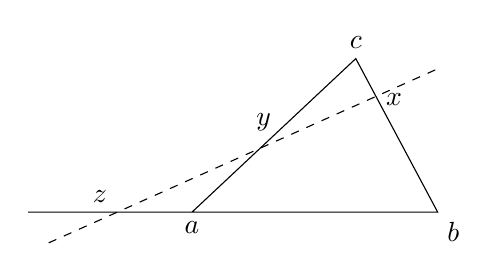
\begin{tikzpicture}[scale=1.3]
      \draw (-1,0)--(3,0)--(2.2, 1.5)--(0.6,0);
      \node[below] at (0.6, 0) {$a$};
      \node[below right] at (3,0) {$b$};
      \node[above] at (2.2, 1.5) {$c$};
      \draw[dashed] (-0.8,-0.3)--(3,1.4);
      \node[above] at (-0.3, 0) {$z$};
      \node[above] at (1.3, 0.7) {$y$};
      \node[right] at (2.4, 1.1) {$x$};
    \end{tikzpicture}\]
    Suppose that they divide these sides in the ratio 
    \[\lambda: 1, \mu: 1, \nu: 1\]
    respectively. Then, the points $x, y, z$ lie on the same line if and only if 
    \[\lambda \mu \nu = -1\]
  \end{corollary}
  \begin{proof}
  By the previous theorem, the points $x, y, z$ are linearly dependent (i.e. lies on a line) if and only if the matrix of barycentric coordinates of $x, y, z$ with respect to $a, b, c$, which is
  \begin{equation}
    \begin{pmatrix}
    0 & \frac{1}{\lambda + 1} & \frac{\lambda}{\lambda + 1} \\
    \frac{\mu}{\mu + 1} & 0 & \frac{1}{\mu + 1} \\
    \frac{1}{\nu + 1} & \frac{\nu}{\nu+1} & 0
    \end{pmatrix}
  \end{equation}
  has nonzero determinant. The determinant of the above matrix is $0$ if and only if $\lambda \mu \nu = -1$. 
  \end{proof}

  \begin{corollary}[Ceva's Theorem]
    In the triangle above, the lines $ax, by, cz$ intersect at one point if and only if 
    \begin{equation}
      \lambda \mu \nu = 1
    \end{equation}
  \end{corollary}
  \begin{proof}
    The proof can be done using barycentric coordinates. 
  \end{proof}

  \begin{theorem}
    A nonempty subset $P \subset S$ is a plane if and only if for any two distinct points $a, b \in P$, the line through $a$ and $b$ also lies in $P$. 
  \end{theorem}

  \begin{theorem}
    Given an inhomogeneous system of linear equations of form 
    \begin{equation}
      A x = b
    \end{equation}
    the set of solutions is an affine plane of dimension $n-r$, where $n$ is the number of variables and $r$ is the rank of the matrix $A$. More precisely, given that the plane is in the form $P = p_0 + U$, $p_0$ is one solution and $U$ is the set of vectors that satisfy the homogeneous system
    \begin{equation}
      Ax = 0
    \end{equation}
  \end{theorem}

  Let us observe the relative position of two planes. 

  \begin{theorem}
    Given two planes 
    \begin{align*}
      P_1 = p_1 + U_1, & P_2 = p_2 + U_2
    \end{align*}
    $P_1$ and $P_2$ intersect if and only if 
    \begin{equation}
      \overline{p_1 p_2} \subset U_1 + U_2
    \end{equation}
    where $U_1 + U_2$ is the set of all vectors of form $u_1 + u_2$, where $u_1 \in U_1, u_2 \in U_2$. 
  \end{theorem}

  Now, consider the class of functions on an affine space corresponding to the class of linear functions on a vector space. 

  \begin{definition}
    An \textbf{affine-linear} function on an affine space $S$ is a function $f: S \longrightarrow \mathbb{F}$ such that
    \begin{equation}
      f(p + x) = f(p) + \alpha (x), \;\; p \in S , x \in V
    \end{equation}
    where $\alpha$, called the \textbf{differential}, is a linear function on the vector space $V$. Let $o \in S$ be a fixed origin. By setting $p = o$, we can express an affine linear function in vectorized form as 
    \begin{equation}
      f(x) = \alpha (x) + b, \;\; b \in \mathbb{F}
    \end{equation}
    where $b = f(o)$. This implies the following coordinate form of $f$. 
    \begin{equation}
      f(x) = b + \sum_i a_i x_i
    \end{equation}
  \end{definition}

  A particular case of affine-linear functions are constant functions, where the defining characteristic is the zero differential. 

  \begin{proposition}
    Given that $\dim{S} = n$, affine-linear functions on $S$ form a $(n+1)$-dimensional subspace on the space of all linear functions on $S$. 
  \end{proposition}

  \begin{proposition}
    Barycentric coordinates are affine-linear functions. 
  \end{proposition}

  \begin{proposition}
    Let $f$ be an affine-linear function. Then
    \begin{equation}
      f \bigg( \sum_i \lambda_i p_i \bigg) = \sum_i \lambda_i f(p_i)
    \end{equation}
    for any barycentric linear combination $\sum_i \lambda_i p_i$ of points $p_1, ..., p_k$. 
  \end{proposition}

  \begin{definition}
    An affine space associated with a Euclidean vector space is called a \textbf{Euclidean affine space}. The \textbf{distance $\rho$} between two points in a Euclidean space is defined as
    \begin{equation}
      \rho(p, q) = ||\overline{pq}||
    \end{equation}
    This definition of $\rho$ satisfies the axioms of a metric space. 
  \end{definition}

\subsection{Convex Sets}

  Let $S$ be an affine space over the field of real numbers and $V$, the associated vector space. 

  \begin{definition}
    The \textbf{(closed) interval} connecting points $p, q \in S$ is the set
    \begin{equation}
      pq = \{\lambda p + (1-\lambda) q \;|\; 0 \leq \lambda \leq 1\}
    \end{equation}
    Geometrically, we can think of this as the straight line segment connecting point $p$ with point $q$. 
  \end{definition}

  \begin{definition}
    A set $M \subset S$ is \textbf{convex} if for any two points $p, q \in S$, it contains the whole interval $p, q$. 
  \end{definition}

  Clearly, the intersection of convex sets is convex. However, the union of them is not. 

  \begin{definition}
    A \textbf{convex linear combination} of points in $S$ is their barycentric linear combination with nonnegative coefficients. 
  \end{definition}

  It is clear to visualize the following proposition. 

  \begin{proposition}
    For any points $p_0, ..., p_k$ in a convex set $M \subset S$, the set $M$ also contains every convex linear combination 
    \begin{equation}
      p = \sum_i \lambda_i p_i
    \end{equation}
    Furthermore, for any set $M \subset S$, the set $\conv{M}$ of all convex linear combinations of points in $M$ is convex. 
  \end{proposition}

  \begin{definition}
    Given $M \subset S$, the set $\conv M$ is the smallest convex set containing $M$. It is called the \textbf{convex hull} of $M$. 
  \end{definition}

  \begin{definition}
    The convex hull of a system of affinely independent points $p_0, p_1, ..., p_n$ in an $n$-dimensional affine space is called the \textbf{$n$-dimensional simplex} with vertices $p_0, ..., p_n$. 
  \end{definition}

  It is clear that the interior points of a simplex is precisely the set of all points whose barycentric coordinates with respect to the vertices are all positive. 

  \begin{example}
    Here are common examples of simplices.
    \begin{enumerate}
      \item A $0$-dimensional simplex is a point. 
      \item A $1$-dimensional simplex is a closed line interval. 
      \item A $2$-dimensional simplex is a triangle. 
      \item A $3$-dimensional simplex is a tetrahedron. 
    \end{enumerate}
  \end{example}

  \begin{proposition}
    A convex set $M$ has interior points if and only if $\aff M = S$. 
  \end{proposition}

  \begin{definition}
    A convex set that has interior points is called a \textbf{convex body}. Clearly, every convex body in $n$-dimensional affine space $S$ is $n$-dimensional. 
  \end{definition}

  The set of interior points of a convex body $M$, denoted $M^\circ$, is an open convex body. 

  \begin{definition}
    For any nonconstant affine-linear function $f$ on the set $S$, let
    \begin{align*}
      H_f \equiv \{p \in S \;|\; f(p) = 0\} \\
      H^+_f \equiv \{p \in S \;|\; f(p) \geq 0\} \\
      H^-_f \equiv \{p \in S \;|\; f(p) \leq 0\}
    \end{align*}
    The set $H_f$ is a hyperplane, and $H^+_f, H^-_f$ are called \textbf{closed half spaces}. 
  \end{definition}

  \begin{definition}
    A hyperplane $H_f$ is a \textbf{supporting hyperplane} of a closed convex body $M$ if $M \subset H^+_f$ and $H_f$ contains at least one (boundary) point of $M$. The half space $H^+_f$ is then called the \textbf{supporting half-space} of $M$. 
  \end{definition}

  \begin{proposition}
    A hyperplane $H$ that passes through a boundary point of a closed convex body $M$, is supporting if and only if $H \cap M^\circ = \emptyset$. 
  \end{proposition}

  A key theorem of convex sets is the following separation theorem. 

  \begin{theorem}[Separation Theorem]
    For every boundary point of a closed convex body, there exists a supporting hyperplane passing through this point. 
  \end{theorem}

  This theorem leads to the following one. 

  \begin{theorem}
    Every closed convex set $M$ is an intersection of (perhaps infinitely many) half-spaces. 
  \end{theorem}

  \begin{definition}
    A \textbf{polyhedron} is the intersection of a finite number of half-spaces. A convex polyhedron which is also a body is called a \textbf{convex solid}. 
  \end{definition}

  \begin{example}
    A simplex with vertices $p_0, p_1, ..., p_n$ is a convex polyhedron since it is determined by linear inequalities $x_i \geq 0$ for $i = 0, 1, ..., n$, where $x_0, x_1, ..., x_n$ are barycentric coordiantes with respect to $p_0, p_1,..., p_n$. 
  \end{example}

  \begin{example}
    A convex polyhedron determined by linear inequalities $0 \leq x_i \leq 1$ for $i = 1, ..., n$, where $x_1,..., x_n$ are affine coordinates with respect ot some frame, is called an $n$-dimensional parallelopiped. 
  \end{example}

  \begin{definition}
    A point $p$ of a convex set $M$ is \textbf{extreme} if it is not an interior point of any interval in $M$. 
  \end{definition}

  \begin{theorem}
    A bounded closed convex set $M$ is the convex hull of the set $E(M)$ of its extreme points. 
  \end{theorem}

  We can create a stronger statement with the following theorem. 

  \begin{theorem}[Minkowski-Weyl Theorem]
    The following properties of a bounded set $M \subset S$ is equivalent.
    \begin{enumerate}
      \item $M$ is a convex polyhedron. 
      \item $M$ is a convex hull of a finite number of points. 
    \end{enumerate}
  \end{theorem}

  \begin{definition}
    A \textbf{face} of a convex polyhedron $M$ is a nonempty intersection of $M$ with some of its supporting hyperplanes. Given that $\dim \aff M = n$, 
    \begin{enumerate}
      \item A $0$-dimensional face is called a \textbf{vertex}. 
      \item A $1$-dimensional face an \textbf{edge}. 
      \item ...
      \item An $(n-1)$-dimensional face a \textbf{hyperface}. 
    \end{enumerate}
  \end{definition}

  Therefore, if a convex polyhedron is determined by a system of linear inequalities, we can obtain its faces by replacing some of these inequalities with equalities (in such a way that we do not get the empty set). 

  The following theorem demonstrates that in order to find its faces, it suffices to consider only the hyperplanes $H_{f_1}, ..., H_{f_m}$. 

  \begin{theorem}
    Every face $\Gamma$ of the polyhedron $M$ is of the form
    \begin{equation}
      \Gamma = M \cap \bigg( \bigcap_{j \in J} H_{f_j} \bigg)
    \end{equation}
    where $J = \{1, 2, ..., m\}$
  \end{theorem}

  \begin{proposition}
    The extreme points of a convex polyhedron $M$ are exactly its vertices. 
  \end{proposition}

  The following theorem is used often in linear programming and in optimization. 

  \begin{theorem}
    The maximum of an affine-linear function on a bounded convex polyhedron $M$ is attained at a vertex. 
  \end{theorem}

\subsection{Affine Transformations and Motions}

  Let $S$ and $S^\prime$ be affine spaces associated with vector spaces $V$ and $V^\prime$, respectively, over the same field $\mathbb{F}$. 

  \begin{definition}
    An \textbf{affine map} from the space $S$ to the space $S^\prime$ is a map $f: S \longrightarrow S^\prime$ such that
    \begin{equation}
      f(p+x) = f(p) + \varphi(x), \;\; p \in S, x \in V
    \end{equation}
    for some linear map $\varphi: V \longrightarrow V^\prime$. It follows that
    \begin{equation}
      \varphi(\overline{pq}) = \overline{f(p) f(q)}, \;\; p, q \in S
    \end{equation}
    Thus, $f$ determines the linear map $\varphi$ uniquely. Similarly, $\varphi$ is called the \textbf{differential} of $f$, denoted $df$. 
  \end{definition}

  \begin{proposition}
    Let $f: S \longrightarrow S^\prime$ and $g: S^\prime \longrightarrow S^{\prime \prime}$ be two affine maps. Then the map
    \begin{equation}
      g \circ f : S \longrightarrow S^{\prime\prime}
    \end{equation}
    is also affine. Also
    \begin{equation}
      d(g \circ f) = dg \cdot df
    \end{equation}
    where $dg$ and $df$ are the differentials of $g$ and $f$, respectively. 
  \end{proposition}

  For $\mathbb{F} = \mathbb{R}$, the differential of an affine map is a particular case of a differential of a smooth map in analysis. That is, the differential is the linear approximation of the function $f$. 

  \begin{proposition}
    An affine map is bijective if and only if its differential is bijective. 
  \end{proposition}

  \begin{definition}
    Similar to linear transformations between vector spaces, bijective affine transformations are called \textbf{isomorphisms} of affine spaces. Affine spaces are \textbf{isomorphic} if there exists an isomorphism between them. 
  \end{definition}

  \begin{corollary}
    Finite-dimensional affine spaces over the same field are isomorphic if and only if they have the same dimension. 
  \end{corollary}

  \begin{definition}
    An affine map from an affine space $S$ to itself is called an \textbf{affine transformation}. Bijective affine transformations form a group called the \textbf{affine group of $S$}, denoted $\GA(S)$. 
  \end{definition}

  It follows that given affine space $S$ with associated vector space $V$, the projection map
  \begin{equation}
    d: \GA(S) \longrightarrow \GL(V)
  \end{equation}
  is a group homomorphism. It's kernel is the group of parallel translations, called Tran$(S)$. 
  \begin{equation}
    t_a : p \mapsto p + a, \;\; a \in V
  \end{equation}

  \begin{proposition}
    For any $f \in \GA(S)$ and $a \in V$, 
    \begin{equation}
      f t_a f^{-1} = t_{df(a)}
    \end{equation}
  \end{proposition}

  \begin{definition}
    A \textbf{homothety} with the center $o$ and coefficient $\lambda$ is an affine transformation defined as
    \begin{equation}
      f( o + x ) \equiv o + \lambda x
    \end{equation}
    In its vectorized form, it is expressed
    \begin{equation}
      f(x) = \lambda x + b, \;\; b \in V
    \end{equation}
    A homothety with coefficient $-1$ is called a \textbf{central symmetry}. 
  \end{definition}

  The group of affine transformations determines the \textbf{affine geometry} of the space. The following theorem shows that all simplices are equal in affine geometry. 

  \begin{theorem}
    Let $\{p_0, ..., p_n\}$ and $\{q_0, ..., q_n\}$ be two systems of affinely independent points in an $n$-dimensional affine space $S$. Then there exists a unique affine transformation $f$ that maps $p_i$ to $q_i$ for $i = 0, 1, ..., n$. 
  \end{theorem}
  \begin{proof}
    It is easy to see once we realize that there exists a unique linear map $\varphi$ of the space $V$ that maps the basis $\{\overline{p_0 p_1}, ..., \overline{p_0 p_n}\}$ to the basis $\{\overline{q_0 q_1}, ..., \overline{q_0 q_n}\}$. If we vectorize $S$ by taking $p_0$ as the origin, the affine transformation in question has the form 
    \begin{equation}
      f(x) = \varphi(x) + \overline{p_0 q_0}
    \end{equation}
  \end{proof}

  \begin{corollary}
    In real affine geometry all parallelopipeds are equal. 
  \end{corollary}

  \begin{definition}
    A \textbf{motion} of the space $S$ is an affine transformation of $S$ whose differential is an orthogonal operator (i.e. an origin preserving isometry). Every motion is bijective. 
  \end{definition}

  Motions of a Euclidean space $S$ form a group denoted Isom$\,S$. A motion is called \textbf{proper (orientation preserving)} if its differential belongs to SO$(V)$ and improper otherwise. 

  \begin{lemma}
    The group Isom$\,S$ is generated by reflections through hyperplanes. 
  \end{lemma}

  \begin{definition}
    Let $M$ be a solid convex polyhedron in an $n$-dimensional Euclidean space. A \textbf{flag of $M$} is a collection of its faces $\{F_0, F_1, ..., F_{n-1}\}$ where $\dim{F_k} = k$ and $F_0 \subset F_1 \subset ... \subset F_{n-1}$. 
  \end{definition}

  \begin{definition}
    A convex polyhedron $M$ is \textbf{regular} if for any two of its flags, there exists a motion $f \in$ Sym$\,M$ mapping the first to the second, where 
    \begin{equation}
      \text{Sym}\,M \equiv \{f \in \text{Isom}\,S \;|\; f(M) = M \}
    \end{equation}
  \end{definition}

  Two dimensional regular polyhedra are the ordinary \textbf{regular polygons}. Their symmetry groups are known as the dihedral groups.

  Three dimensional regular polyhedra are \textbf{Platonic solids}, which are the regular tetrahedron, cube, octahedron, dodecahedron, and icosahedron. 

  \begin{definition}
    A real vector space $V$ with a fixed symmetric bilinear function $\alpha$ of signature $(k, l)$, where $k, l > 0$ and $\dim{V} = k+l$, is called the \textbf{pseudo-Euclidean vector space} of signature $(k, l)$. The group of $\alpha$-preserving linear transformations of $V$ is called the \textbf{pseudo-orthogonal group} and is denoted O$(V, \alpha)$. In an orthonormal basis, the corresponding matrix group is denoted $O{k,l}$. 
  \end{definition}

\subsection{Quadrics}

  Planes are the simplest objects of affine and Euclidean geometry, which are determined by systems of linear equations. The second simplest are quadratic functions. These types of objects are studied futher in algebraic geometry. 

  \begin{definition}
    An \textbf{affine-quadratic function} on an affine space $S$ is a function $Q: S \longrightarrow \mathbb{F}$ such that its vectorized form is
    \begin{equation}
      Q(x) = q(x) + l(x) + c
    \end{equation}
    for a quadratic function $q$, linear function $l$, and constant $c$. 
  \end{definition}

\subsection{Projective Spaces}

  \begin{definition}
    An $n$-dimensional \textbf{projective space $PV$} over a field $\mathbb{F}$ is the set of one-dimensional subspaces of an $(n+1)$-dimensional vector space $V$ over $\mathbb{F}$. For every $(k+1)$-dimensional subspace $U \subset V$, the subset $PU \subset PV$ is called a $k$-dimensional \textbf{plane} of the space $PV$. 
    \begin{enumerate}
      \item $0$-dimensional planes are the points of $PV$. 
      \item $1$-dimensional planes are called \textbf{lines}
      \item ...
      \item $(n-1)$-dimensional planes are called \textbf{hyperplanes}
    \end{enumerate}
  \end{definition}

  \begin{definition}
    $\mathbb{RP}^1$ is called the real projective line, which is topologically equivalent to a circle. 
  \end{definition}

  \begin{example}
    The real projective space of $\mathbb{R}^2$ is the set of all lines that pass through the origin. It is denoted $\mathbb{R P}^2$ and called the \textbf{real projective plane}. 
  \end{example}

  \begin{example}
    $\mathbb{RP}^3$ is diffeomorphic to SO$(3)$. 
  \end{example}

  \begin{example}
    The space $\mathbb{RP}^n$ is formed by taking the quotient of $\mathbb{R}^{n+1} \setminus \{0\}$ under the equivalence relation 
    \begin{equation}
      x \sim \lambda x \text{ for all real numbers } \lambda \neq 0
    \end{equation}
    The set of these equivalence classes is isomorphic to $\mathbb{RP}^n$. 
  \end{example}


\section{Representations}

  We will assume that $V$ is a finite-dimensional vector space over field $\mathbb{C}$. 

  \begin{definition}
    The \textbf{general linear group} of vector space $V$, denoted $\GL(V)$, is the group of all automorphisms of $V$ to itself. The \textbf{special linear group} of vector space $V$, denoted $\SL(V)$ is the subgroup of automorphisms of $V$ with determinant $1$. 
  \end{definition}

  When studying an abstract set, it is often useful to consider the set of all maps from this abstract set to a well known set (e.g. $\GL(V)$). 

  \begin{definition}
    A \textbf{representation} of an (algebraic) group $\mathcal{G}$ is a homomorphism 
    \begin{equation}
      \rho: G \longrightarrow \GL(V)
    \end{equation}
    for some vector space $V$. That is, given an element $g \in \mathcal{G}$, $\rho(g) \in \GL (V)$, meaning that $\rho(g)(v) \in V$. Additionally, since it is a homomorphism, the algebraic structure is preserved. 
    \begin{equation}
      \rho(g_1 \cdot g_2) = \rho(g_1) \cdot \rho(g_2)
    \end{equation}
    where $\cdot$ on the left hand side is the abstract group multiplication while the $\cdot$ on the right hand side is matrix multiplication. To shorten the notation, we will denote 
    \begin{equation}
      g v = \rho(g) v, \; v \in V
    \end{equation}
    Since $\rho$ is a group morphism, we have 
    \begin{equation}
      g_2 (g_1 v) = (g_2 g_1) v \; \iff \rho(g_2) \big( \rho(g_1) (v) \big) = \big( \rho(g_2) \rho(g_1) \big) (v)
    \end{equation}
    Additionally, since $g$ (that is, $\rho(g)$) is a linear map, 
    \begin{equation}
      g(\lambda_1 v_1 + \lambda_2 v_2) = \lambda_1 g v_1 + \lambda_2 g v_2
    \end{equation}
    Usually, we refer to the map as the representation, but if the map is well-understood, we just call the vector space $V$ the representation and say that the group acts on this vector space. 
  \end{definition}

  \begin{example}
    The group $\GL(2, \mathbb{C})$ can be represented a by the vector space $\mathbb{C}^2$, or explicitly, by the group of $2 \times 2$ matrices over $\mathbb{C}$ with nonzero determinant.
    \begin{equation}
      \GL(2, \mathbb{C}) \xmapsto{id} \text{Mat}(2, \mathbb{C})
    \end{equation}
    This is a trivial representation. 
  \end{example}

  We now show a nontrivial representation of $\GL(2, \mathbb{C})$. 

  \begin{example}
    We take Sym$^2 \mathbb{C}^2$, the second symmetric power of $\mathbb{C}^2$. Note that given a basis $x_1, x_2 \in \mathbb{C}^2$, the set
    \begin{equation}
      \{x_1 \odot x_1, x_1 \odot x_2, x_2 \odot x_2\}
    \end{equation}
    forms a basis of Sym$^2 \mathbb{C}^2 \implies \dim\,$Sym$^2 \mathbb{C}^2 = 3$. So, we want to represent $\GL(2, \mathbb{C})$ by associating its element with elements of $\GL(Sym^2 \mathbb{C}^2)$. More concretely, we are choosing to represent a $2 \times 2$ matrix over $\mathbb{C}$ with a $3 \times 3$ matrix group (since $\GL(Sym^2 \mathbb{C}^2) \simeq \GL(3, \mathbb{C})$. Clearly,
    \begin{align*}
      & \rho(g) (x_1 \odot x_1) = g(x_1) \odot g(x_1) \in Sym^2 \mathbb{C}^2 \\
      & \rho(g) (x_1 \odot x_2) = g(x_1) \odot g(x_2) \\
      & \rho(g) (x_2 \odot x_2) = g(x_2) \odot g(x_2)
    \end{align*}
    To present this in matrix form, let us have an element in $\GL (2, \mathbb{C})$
    \begin{equation}
      \mathcal{A} \equiv \begin{pmatrix}
      a & b \\
      c & d
      \end{pmatrix}
    \end{equation}
    We evaluate the corresponding representation in $\GL( Sym^2 \mathbb{C}^2)$. Using the identities above, we have 
    \begin{align*}
      \rho(g) (x_1 \odot x_1) & = g(x_1) \odot g(x_1) \\
      & = (a x_1 + c x_2) \odot (a x_1 + c x_2) \\
      & = a^2 x_1 \odot x_1 + 2ac x_1 \odot x_2 + c^2 x_2 \odot x_2 \\
      \rho(g) (x_1 \odot x_2) & = g(x_1) \odot g(x_2) \\
      & = (a x_1 + c x_2) \odot (b x_1 + d x_2) \\
      & = ab x_1 \odot x_1 + (ad + bc) x_1 \odot x_2 + cd x_2 \odot x_2 \\
      \rho(g) (x_2 \odot x_2) & = g(x_2) \odot g(x_2) \\
      & = (b x_1 + d x_2) \odot (b x_1 + d x_2) \\
      & = b^2 x_1 \odot x_1 + 2bd x_1 \odot x_2 + d^2 x_2 \odot x_2
    \end{align*}
    And this completely determines the matrix. So, 
    \begin{equation}
      \rho \begin{pmatrix}
      a&b\\c&d
      \end{pmatrix} = \begin{pmatrix}
      a^2&ab&b^2\\2ac&ad+bc&2bd\\c^2&cd&d^2
      \end{pmatrix}
    \end{equation}
    is the $3 \times 3$ representation of $\mathcal{A}$ in $\GL(Sym^2 \mathbb{C}^2)$. 
  \end{example}

  We continue to define maps between two representations of $\mathcal{G}$. 

  \begin{definition}
    A \textbf{morphism} between 2 representations 
    \begin{align*}
      & \rho_1: \mathcal{G} \longrightarrow \GL(V_1) \\
      & \rho_2: \mathcal{G} \longrightarrow \GL(V_2) 
    \end{align*}
    of some group but not necessarily the same vector space is a linear map $f: V_1 \longrightarrow V_2$ that is \textbf{compatible} with the group action. That is, $f$ satisfies the property that for all $g \in \mathcal{G}$
    \begin{equation}
      f \circ g = g \circ f
    \end{equation}
    Again, we use the shorthand notation that $g = \rho(g)$, meaning that the statement above really translates to $ f \circ \rho(g) = \rho(g) \circ f$. This is equivalent to saying that the following diagram commutes. 
    \[\begin{tikzcd}
    V_1 \arrow{r}{\rho_1(g)} \arrow{d}{f} & V_1 \arrow{d}{f} \\
    V_2 \arrow{r}{\rho_2 (g)} & V_2
    \end{tikzcd}\]
  \end{definition}

  \begin{definition}
    Let $V$ be a representation of $\mathcal{G}$. A \textbf{subrepresentation} is a subspace $W \subset V$ such that for all $g \in \mathcal{G}$ and for all $w \in W$, 
    \begin{equation}
      \rho(g)(w) \in W
    \end{equation}
  \end{definition}

  \begin{example}
    $V$ and $\{0\}$ are always subrepresentations of $V$. 
  \end{example}

  We now introduce the "building blocks" of all representations. 
  \begin{definition}
    A representation $W$ is \textbf{irreducible representation} if $\{0\}$ and $W$ are the only subrepresentations of $W$. 
  \end{definition}

  \begin{lemma}[Schur's Lemma]
    Let $V_1, V_2$ be irreducible representations and let $f: V_1 \longrightarrow V_2$ be a morphism (of representations). Then, either
    \begin{enumerate}
      \item $f$ is an isomorphism. 
      \item $f = 0$
    \end{enumerate}
    Furthermore, any 2 isomorphisms differ by a constant. That is, 
    \begin{equation}
      f_1 = \lambda f_2
    \end{equation}
  \end{lemma}
  \begin{proof}
    $\ker{f}$ is clearly a vector space. Furthermore, it is a subrepresentation (since it is a subspace of $V_1$) $\implies \ker{f} = V$ or $\ker{f} = 0$. If $\ker{f} = V$, then $f = 0$ and the theorem is satisfied. If $\ker{f} = 0$, then $f$ is injective, and $\im{f}$ is a subrepresentation of $V_2 \implies \im{f} = 0$ or $\im{f} = V_2$. But $\im{f} \neq 0$ since $f$ is injective, so $\im{f} = V_2 \implies f$ is surjective $\implies f$ is bijective, that is, $f$ is an isomorphism of vector spaces. So, the inverse $f^{-1}$ exists, and this map $f^{-1}$ satisfies
    \begin{equation}
      f^{-1} \circ \rho_2(g) = \rho_1 (g) \circ f^{-1}
    \end{equation}
    To prove the second part, without loss of generality, assume that the first isomorphism is the identity mapping. That is, 
    \begin{equation}
      f_1 = id
    \end{equation}
    Since we are working over the field $\mathbb{C}$, we can find an eigenvector of $f_2$. That is, there exists a $v \in V_1$ such that 
    \begin{equation}
      f_2 (v) = \lambda v
    \end{equation}
    Now, we define the map
    \begin{equation}
      f: V_1 \longrightarrow V_2, \; f \equiv f_2 - \lambda f_1
    \end{equation}
    Clearly, $\ker{f} \neq 0$, since $v \in \ker{f}$. That is, we have a map $f$ between 2 irreducible representations that has a nontrivial kernel. This means that $f = 0 \implies f_2 = \lambda f_1$.  
  \end{proof}

  \begin{theorem}[Mache's Theorem]
    Let $V$ be finite dimensional, with $\mathcal{G}$ a finite group. Then, $V$ can be decomposed as 
    \begin{equation}
      V = \bigoplus_{i} V_i
    \end{equation}
    where each $V_i$ is an irreducible representation of $\mathcal{G}$. 
  \end{theorem}
  \begin{proof}
    By induction on dimension, it suffices to prove that if $W$ is a subrepresentation of $V$, then there exists a subrepresentation $W^\prime \subset V$ such that $W \oplus W^\prime = V$. So, if $V$ isn't an irreducible representation, it can always be decomposed into smaller subrepresentations $W$ and $W^\prime$ that direct sum to $V$. Now, we define the canonical (linear) projection 
    \begin{equation}
      \pi: V \longrightarrow W
    \end{equation}
    Then, we define the new map 
    \begin{equation}
      \Tilde{\pi}: V \longrightarrow W, \; \Tilde{\pi}(v) \equiv \frac{1}{|\mathcal{G}|} \sum_{g \in \mathcal{G}} \rho(g)\big|_W \circ \pi \circ \rho(g)^{-1}
    \end{equation}
    This "averaging" of the group elements are done so that this mapping is a map of representations. This implies that 
    \begin{equation}
      V = W \oplus \ker{\Tilde{\pi}}
    \end{equation}
    meaning that $V$ can indeed be decomposed into direct sums of subrepresentations. 
  \end{proof}


\section{Lie Groups and Lie Algebras}

  \begin{definition}
    A \textbf{Lie group} is a group $\mathcal{G}$ that is also a finite-dimensional smooth manifold, in which the group operations of multiplication and inversion are smooth maps. Smoothness of the group multiplication
    \begin{equation}
      \mu: \mathcal{G} \times \mathcal{G} \rightarrow \mathcal{G}, \; \mu(x, y) = x y
    \end{equation}
    means that $\mu$ is a smooth mapping of the product manifold $\mathcal{G} \times \mathcal{G}$ into $\mathcal{G}$. These two requirements can be combined to the single requirement that tahe mapping 
    \begin{equation}
      (x, y) \mapsto x^{-1} y
    \end{equation}
    be a smooth mapping of the product manifold into $\mathcal{G}$. 
  \end{definition}

  \begin{definition}
    A \textbf{Lie Algebra} is a vector space $\mathfrak{g}$ with an operation called the \textbf{Lie Bracket} 
    \begin{equation}
      [\cdot, \cdot]: \mathfrak{g} \times \mathfrak{g} \rightarrow \mathfrak{g}
    \end{equation}
    Satisfying
    \begin{enumerate}
      \item Bilinearity: $[ax + by, z] = a[x,z] + b[y,z], \; [z, ax + by] = a[z, x] + b[z,y]$
      \item Anticommutativity: $[x,y] = -[y,x]$
      \item Jacobi Identity: $[x,[y,z]] + [y,[z,x]] + [z,[x,y]] = 0$
    \end{enumerate}
    Clearly, this implies that $\mathfrak{g}$ is a nonassociative algebra. Note that a Lie Algebra does not necessarily need to be an algebra in the sense that there needs to be multiplication operation that is closed in $\mathfrak{g}$. 
  \end{definition}

  \begin{example}
    A common example of a Lie Braket in the algebra of matrices is defined
    \begin{equation}
      [A, B] \equiv AB - BA
    \end{equation}
    called the \textbf{commutator}. Note that in this case, the definition of the Lie bracket is dependent on the definition of the matrix multiplication. Without defining the multiplication operation, we wouldn't know what $AB$ or $BA$ means. Therefore, we see that the Lie algebra of $n \times n$ matrices has three operations: matrix addition, matrix multiplication, and the commutator (along with scalar multiplication). But in general, it is not necessary to have that multiplication operation for abstract Lie algebras. $\mathfrak{g}$ just needs to be a vector space with the bracket.  
  \end{example}

  \begin{example}
    The set of all symmetric matrices is a vector space, but it is \textbf{not} a Lie algebra since the commutator $[A,B]$ is not symmetric unless $A B = B A$. 
  \end{example}

  We will first talk about groups of matrices as a more concerete example before we get into abstract Lie groups. Recall that the matrix exponential map is defined
  \begin{equation}
    exp: \text{Mat}(n, \mathbb{C}) \rightarrow \text{mat}(n, \mathbb{C}), \; exp(A) = e^A = \sum_{p \geq 0} \frac{A^p}{p!}
  \end{equation}
  Note that this value is always well defined. This lets us define
  \begin{equation}
    exp(t A) \equiv e^{t A} \equiv I + tA + \frac{1}{2} t^2 A^2 + \frac{1}{3!} t^3 A^3 + ... 
  \end{equation}
  where if $t$ is small, we can expect a convergence. Note that exp maps addition to multiplication. That is, we can interpret it as a homomorphism from 
  \begin{equation}
    exp: \mathfrak{g} \rightarrow \mathcal{G}
  \end{equation}
  where $\mathfrak{g}$ is the Lie algebra and $\mathcal{G}$ is the Lie group (which we will treat just as a matrix group). To find the inverse of the exponential map, we can take the derivative of $e^{tA}$ at $t=0$. That is, 
  \begin{align*}
    \bigg(\frac{d}{d t} e^{tA} \bigg) \bigg|_{t=0} & = \bigg(\sum_{k=0}^\infty \frac{1}{k!} t^k A^{k+1} \bigg) \bigg|_{t=0} = A
  \end{align*}
  So, the mapping
  \begin{equation}
    \frac{d}{dt} \bigg|_{t=0}: \mathcal{G} \rightarrow \mathfrak{g}
  \end{equation}
  maps the Lie group back to the algebra. We can interpret this above mapping by visualizing the Lie Algebra as a tangent (vector) space of the abstract Lie group $\mathcal{G}$ at the identity element of the Lie group. The visualization below isn't the most abstract one, but it may help:

  \begin{figure}[H]
    \centering 
    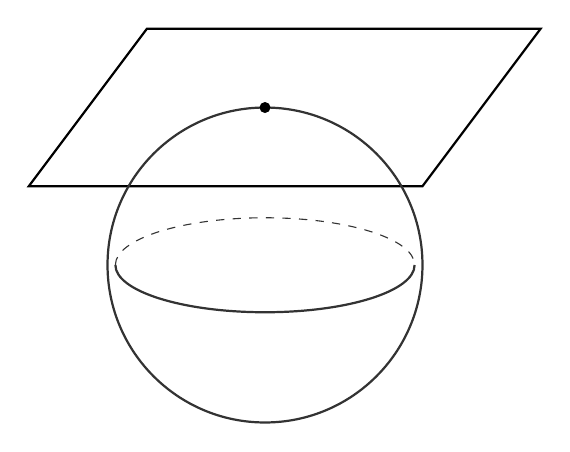
\begin{tikzpicture}[scale=1]
      % Define colors
      \colorlet{spherecol}{black!80}
      \colorlet{arrowcol}{cyan!70!blue}
      
      % Draw the tangent plane (Lie Algebra)
      \draw[thick] (-1.5,3) -- (3.5,3) -- (2,1) -- (-3,1) -- cycle;
      
      % Draw the sphere (Lie Group)
      \draw[spherecol, thick] (0,0) circle (2cm);
      \draw[spherecol, thick] (-1.9,0) arc (180:360:1.9cm and 0.6cm);
      \draw[spherecol, dashed] (-1.9,0) arc (180:0:1.9cm and 0.6cm);
      
      % Identity element
      \fill (0,2) circle (0.07cm);
    \end{tikzpicture}
    \caption{The Lie algebra can be visualized as the tangent space at the identity.} 
    \label{fig:lie_algebra_tangent_space}
  \end{figure}

  For example, say that the Lie group $\mathcal{G}$ is a unit circle in $\mathbb{C}$, then the Lie algebra of $\mathcal{G}$ is the tangent space at the identity $1$, which can be identified as the imaginary line in the complex plane $\{i t \; | \; t \in \mathbb{R}\}$, with 
  \begin{equation}
    i t \mapsto exp(it) \equiv e^{it} \equiv \cos{t} + i \sin{t}
  \end{equation}

  \begin{center}
    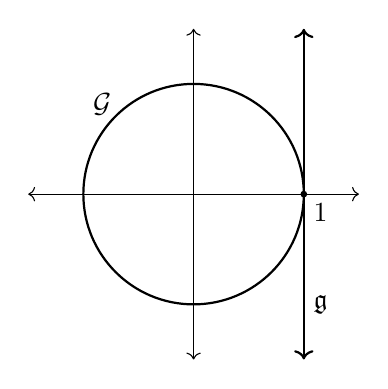
\begin{tikzpicture}[scale=0.7]
      \draw[thick] (0,0) circle (2);
      \node[below right] at (-2,2) {$\mathcal{G}$};
      \draw[<->] (-3,0)--(3,0);
      \draw[<->] (0,-3)--(0,3);
      \draw[fill] (2,0) circle (0.05);
      \node[below right] at (2,0) {$1$};
      \draw[thick, <->] (2,-3)--(2,3);
      \node[right] at (2,-2) {$\mathfrak{g}$};
    \end{tikzpicture}
  \end{center}
  So, analyzing the Lie group by looking at its Lie algebra turns a nonlinear problem to a linear one; this is called a \textbf{linearization} of the Lie group. The existence of this exponential map is one of the primary reasons that Lie algebras are useful for studying Lie groups. 

  \begin{example}
    The exponential map 
    \begin{equation}
      exp: \mathbb{R} \rightarrow \mathbb{R}^+, \; x \mapsto e^x
    \end{equation}
    is a group homomorphism that maps $(\mathbb{R}, +)$ to $(\mathbb{R}^+, \times)$. This means that $\mathbb{R}$ is the Lie algebra of the Lie group $\mathbb{R}^+$. 
  \end{example}

  \begin{theorem}
    If $A$ and $B$ are commuting square matrices, then 
    \begin{equation}
      e^{A + B} = e^A \, e^B
    \end{equation}
    In general, the solution $C$ to the equation
    \begin{equation}
      e^{A} \, e^B = e^C
    \end{equation}
    is given by the \textbf{Baker-Campbell-Hausdorff formula}, defined
    \begin{equation}
      C = A + B + \frac{1}{2}[A,B] + \frac{1}{12} [A,[A,B]] - \frac{1}{12} [B,[A,B]] + ...
    \end{equation}
    consisting of terms involving higher commutators of $A$ and $B$. The full series is much too complicated to write, so we ask the reader to be satisfied with what is shown. 
  \end{theorem}

  The BCH formula is messy, but it allows us to compute products in the Lie Group as long as we known the commutators in the Lie Algebra. 

  Therefore, we can describe the process of constructing a Lie group from a Lie Algebra (which a vector space) as such. We take a vector space $V$ and endow it the additional bracket operation. We denote this as
  \begin{equation}
    \mathfrak{g} \equiv (V, [\cdot, \cdot])
  \end{equation}
  Then, we take every element of $\mathfrak{g}$ and apply the exponential map to them to get an another set $\mathcal{G}$. We then endow a group structure on $\mathcal{G}$ by defining the multiplication as 
  \begin{equation}
    \cdot: \mathcal{G} \times \mathcal{G} \rightarrow \mathcal{G}, \; e^A \cdot e^B = e^{A * B}
  \end{equation}
  where $A*B$ is defined by the BCH formula up to a certain $k$th order. Since the $*$ operation is completely defined by the bracket in the Lie algebra, it tells us how to multiply in the Lie group. This process can be made more abstractly, depending on what $A, B$ and $[\cdot,\cdot]$ is, beyond matrices. 

\subsection{Lie Algebras of Classical Lie Groups}

  \begin{definition}[General Linear Group]
    The \textbf{general linear group}, denoted GL$(V)$, is the set of all bijective linear mappings from $V$ to itself. Similarly, GL$_{n}(\mathbb{F})$, or GL $(n, \mathbb{F})$ is the set of all nonsingular $n \times n$ matrices over the field $\mathbb{F}$. Due to the same dimensionality of the following spaces, it is clear that GL$(V) \simeq$ GL$(\mathbb{F}^{n}) \simeq$ GL$_{n}(\mathbb{F})$. The \textbf{special linear group}, denoted SL$_{n} (\mathbb{F})$ or SL$(n, \mathbb{F})$, is the set of $n\times n$ matrices a with determinant $1$. SL$_{n}(\mathbb{F})$ is a subgroup of GL$_{n}(\mathbb{F})$, which is a subset of the ring of all $n \times n$ matrices over field $\mathbb{F}$, denoted $\mathbb{L}_{n}(\mathbb{F})$. 
  \end{definition}

  \begin{definition}[Translation Group]
    The group of all translations in the space $V$ is denoted Tran$\,V$. Its elements are usually denoted as $t_{u}$, where $u$ is the vector that is being translated by. It can also be interpreted as shifting the origin by $-u$. It is clear that Tran$\,V \simeq V$. 
  \end{definition}

  \begin{definition}[General Affine Group]
    The \textbf{general affine group} is the pair of all transformations
    \begin{equation}
      \text{GA} (V) \equiv \text{Tran}(V) \times \text{GL}(V)
    \end{equation}
  \end{definition}

  \begin{definition}[Isometries]
    The \textbf{Euclidean group} of \textbf{isometries} in the Euclidean space $\mathbb{E}^{n}$ (with the Euclidean norm), denoted Isom$\, \mathbb{E}^{n}$ or $\mathbb{E}(n)$, consists of all distance-preserving bijections from $\mathbb{E}^{n}$ to itself, called \textbf{motions} or \textbf{rigid transformations}. It consists of all combinations of rotations, reflections, and translations. The \textbf{special Euclidean group} of all isometries that preserve the \textbf{handedness} of figures is denoted $\mathbb{SE}(n)$, which is comprised of all combinations rotations and translations called \textbf{rigid motions} or \textbf{proper rigid transformations}.
  \end{definition}

  \begin{definition}[Orthogonal Group]
    The \textbf{orthogonal group}, denoted $\O(n)$, consists of all isometries that preserve the origin, i.e. consists of rotations and reflections. The \textbf{special orthogonal group}, denoted SO$(n)$, is a subgroup of O$(n)$ consisting of only rotations. We can see that 
    \begin{equation}
      \text{O}(n)=\frac{\text{Isom}\, \mathbb{E}^{n}}{\text{Tran}\,V}
    \end{equation}
  \end{definition}

  \begin{definition}[Transitive]
    A transformation group $G$ is called \textbf{transitive} if for any $x, y \in X$, there exists a $\phi \in G$ such that $y = \phi(x)$. 
  \end{definition}

  \begin{example}
    Tran$(V)$ and GA$(V)$ are transitive groups. 
  \end{example}

  \begin{definition}[Congruence Classes]
    Let $X$ be a set and $G$ its transformation group on $X$. The way we define $G$ determines the \textbf{geometry} of $X$. More specifically, a figure $F_{1} \subset X$ is \textbf{equivalent} or \textbf{congruent} to $F_{2} \subset X$ iff there exists $\phi \in G$ such that $F_{2} = \phi (F_{1})$ (or equivalently, $F_{1} = \phi (F_{2})$). This is an equivalence relation since
    \begin{enumerate}
      \item $F \sim F$. 
      \item $F \sim H \implies H \sim F$. 
      \item $F \sim H, H \sim K \implies F \sim K$
    \end{enumerate}
    Two figures that are in the same equivalence class are known to be \textbf{congruent} with respect to the geometry of $X$ induced by $G$. 
  \end{definition}

  Clearly, if two figures are congruent in Euclidean geometry, then they are congruent in Affine geometry, since E$(n) \subset$ GA$(n)$. 


\subsubsection[Lie Algebras of SL(2, R) and SL(2, C)]{Lie Algebras of $\SL(2, \mathbb{R})$ and $\SL(2, \mathbb{C})$}

  Given the group $\SL(2, \mathbb{R})$, there must be a corresponding Lie algebra of matrices such that $g = e^A \in \SL(2, \mathbb{R})$. We attempt to find this Lie algebra. Let $g \in \SL(2, \mathbb{R})$, with $g = e^A$. So, if $\det{g} = 1$, what is the corresponding restriction on $A$ in the algebra? We use the following theorem. 

  \begin{theorem}
    \begin{equation}
      \det{(e^A)} = e^{\Tr{(A)}}
    \end{equation}
  \end{theorem}
  \begin{proof}
    Put $A$ in Jordan Normal Form: $A = S^{-1} J S \implies A^n = S^{-1} J^n S \implies exp(A) = S^{-1} exp(A) S \implies \det{(exp(A))} = \det{e^J}$. But since $J$ is upper trianglar, $J^n$ is upper triangular $\implies e^J$ is upper triangular, which implies that 
    \begin{equation}
      \det{e^J} = \prod_i e^{\lambda_i} = e^{\Tr{(J)}} = e^{\Tr{(A)}}
    \end{equation}
    since trace is invariant under a change of basis. 
  \end{proof}

  So, $\det{(e^A)} = 1 \implies \Tr{(A)} = 2 \pi i n$ for $n \in \mathbb{Z}$. Since we want to component connected to the identity, we choose $n=0$ meaning that $\Tr{(A)} = 0$. And we are done. That is, the Lie algebra of $\SL(2, \mathbb{R})$ consists of traceless $2 \times 2$ matrices, denoted $\mathfrak{sl}_2 \mathbb{R}$. $\mathfrak{sl}_2 \mathbb{R}$ has basis (chosen arbitrarily) 
  \begin{equation}
    \bigg\{ H = \begin{pmatrix}
    1&0\\0&-1
    \end{pmatrix}, X = \begin{pmatrix}
    0&1\\0&0
    \end{pmatrix}, Y = \begin{pmatrix}
    0&0\\1&0
    \end{pmatrix}\bigg\}
  \end{equation}
  and the identity in the Lie algebra is the zero matrix, which translates to the $2 \times 2$ identity matrix in the Lie group. 
  \begin{equation}
    exp \begin{pmatrix}
    0&0\\0&0
    \end{pmatrix} = I
  \end{equation}
  We must not forget to define the bracket structure in $\mathfrak{sl}_2 \mathbb{R}$, so we define it as the commutator, which gives the identity
  \begin{align*}
    & [H,X] = HX - XH = 2X \\
    & [H,Y] = HY - YH = -2Y \\
    & [X,Y] = XY - YX = H
  \end{align*}
  Note that regular matrix multiplication is not closed within this Lie algebra. For example, 
  \begin{equation}
    X Y = \begin{pmatrix}
    1&0\\0&0
    \end{pmatrix}
  \end{equation}
  is clearly not traceless. However, the bracket operation keeps the matrices within this traceless condition (and thus, within this algebra), so you can't just stupidly multiply matrices together in a Lie algebra. Remember that regular matrix multiplication does not have anything to do with the Lie bracket and does not apply to this group. This algebra also simplifies the multiplicative inverse of a group to a simple additive inverse, making calculations easier. 

  Similarly, the Lie algebra of $\SL(2, \mathbb{C})$ also has the same basis 
  \begin{equation}
    \bigg\{ H = \begin{pmatrix}
    1&0\\0&-1
    \end{pmatrix}, X = \begin{pmatrix}
    0&1\\0&0
    \end{pmatrix}, Y = \begin{pmatrix}
    0&0\\1&0
    \end{pmatrix}\bigg\}
  \end{equation}
  but we choose the field to be $\mathbb{C}$, meaning that we take complex linear combinations rather than real linear ones. 

\subsubsection[Lie Algebra of SU(2)]{Lie Algebra of \(\SU(2)\)}

  $g \in $ SU$(2) \implies \det{g} = 1 \implies \Tr{A} = 0$. We also see that by definition $e^A$, 
  \begin{equation}
    (e^A)^\dagger = e^{A^\dagger} \text{ and } (e^A)^{-1} = e^{-A}
  \end{equation}
  which implies that $A^\dagger = - A$. That is, the unitary condition implies that the Lie algebra elements in $\mathfrak{su}(2)$ are traceless, anti-self adjoint $2 \times 2$ matrices over $\mathbb{C}$. 

  \begin{definition}
    The \textbf{Pauli matrices} are the three matrices
    \begin{equation}
      \bigg\{ \sigma_x = \begin{pmatrix}
      0&1\\1&0
      \end{pmatrix}, \sigma_y = \begin{pmatrix}
      0&-i\\i&0
      \end{pmatrix}, \sigma_z = \begin{pmatrix}
      1&0\\0&-1
      \end{pmatrix}\bigg\}
    \end{equation}
    Note that with some calculation, 
    \begin{align*}
      & [\sigma_x, \sigma_y] = 2 i \sigma_z \\
      & [\sigma_y, \sigma_z] = 2 i \sigma_x \\
      & [\sigma_z, \sigma_x] = 2 i \sigma_y
    \end{align*}
  \end{definition}

  To identify the basis of $\mathfrak{su}(2)$, we take the Pauli matrices and let 
  \begin{align*}
    & A_x \equiv - \frac{i}{2} \sigma_x = \begin{pmatrix} 0&-i/2\\-i/2&0 \end{pmatrix} \\
    & A_y \equiv - \frac{i}{2} \sigma_y = \begin{pmatrix}0&-1/2\\1/2&0\end{pmatrix} \\
    & A_z \equiv -\frac{i}{2} \sigma_z = \begin{pmatrix}-i/2&0\\0&i/2\end{pmatrix}
  \end{align*} 
  be the basis of $\mathfrak{su}(2)$. Clearly, $A_x, A_y, A_z$ are all traceless, anti-self adjoint $2 \times 2$ matrices. Moreover, they also satisfy
  \begin{align*}
    & [A_x, A_y] = A_z \\
    & [A_y, A_z] = A_x \\
    & [A_z, A_x] = A_y
  \end{align*}
  However, note that the algebra $\mathfrak{su}(2)$ consists of all \textbf{real} linear combinations of $A_x, A_y, A_z$. That is, $\mathfrak{su}(2)$ is a 3 dimensional \textbf{real} vector space, even though it has basis elements containing complex numbers. 

  However, we can always complexify this space by simply replacing real scalar multiplication in $\mathfrak{su}(2)$ with complex scalar multiplication. By complexifying $\mathfrak{su}(2)$, the Lie group SU$(2)$ formed by taking the exponential map on this complexified space is actually identical to $\SL(2, \mathbb{C})$. Indeed, this is true because first, the basis $\{H, X, Y\}$ of $\mathfrak{sl}_2 \mathbb{C}$ and the basis $\{A_x, A_y, A_z\}$ of $\mathfrak{su}(2)$ span precisely the same subspace in the vector space Mat$(2, \mathbb{C})$, meaning that the two Lie algebras are the same vector space. Secondly, the bracket operation $[\cdot, \cdot]$ in both $\mathfrak{sl}_2 \mathbb{C}$ and $\mathfrak{su}(2)$ are equivalent since the operation defined to be the commutator in both cases, resulting in the similarities in the bracket behaviors. 
  \begin{align*}
    [H,X] = 2X & \iff [A_x, A_y] = A_z \\
    [H,Y] = - 2Y & \iff [A_y, A_z] = A_x\\
    [X,Y] = H & \iff  [A_z, A_x] = A_y 
  \end{align*}
  Therefore, the complexification of SU$(2)$ and $\SL(2, \mathbb{R})$ both leads to the construction of $\SL(2, \mathbb{C})$. 

  \begin{center}
    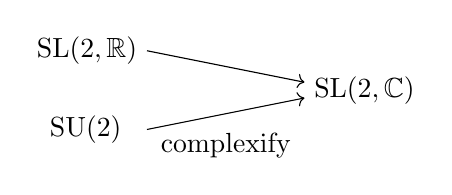
\begin{tikzpicture}
      \node[left] at (0,0.5) {$\SL(2, \mathbb{R})$};
      \node[left] at (-0.2,-0.5) {SU$(2)$};
      \node[right] at (2,0) {$\SL(2,\mathbb{C})$};
      \draw[->] (0,0.5)--(2,0.1);
      \draw[->] (0,-0.5)--(2,-0.1);
      \node at (1,-0.7) {complexify};
    \end{tikzpicture}
  \end{center}
  We can interpret the "real forms" of $\SL(2, \mathbb{C})$ as "slices" of some complex group. However, this does not mean that the real version of these groups are equal. That is, 
  \begin{equation}
    \SL(2, \mathbb{R}) \neq \text{SU}(2)
  \end{equation}

\subsubsection{Lie Algebra of SO(3)}

  It is easy to see that for SO$(2)$, it is easy to see that its Lie algebra $\mathfrak{so}(2)$ has 
  \begin{equation}
    \bigg\{ \begin{pmatrix}
    0&-1\\1&0
    \end{pmatrix}\bigg\}
  \end{equation}
  as its only basis, since 
  \begin{equation}
    exp  \bigg( \begin{pmatrix}
    0&-1\\1&0
    \end{pmatrix} \theta \bigg) = \begin{pmatrix}
    \cos{\theta} & - \sin{\theta} \\
    \sin{\theta} & \cos{\theta}
    \end{pmatrix}
  \end{equation}
  meaning that the dimension of SO$(2)$ is $1$. By adding a component, we can get a rotation in $\mathbb{R}^3$. 
  \begin{align*}
    & R_x = \begin{pmatrix}0&0&0\\0&0&-1\\0&1&0\end{pmatrix} \implies e^{R_x} = \begin{pmatrix}
    1&0&0\\ 0&\cos{\theta}&-\sin{\theta}\\0&\sin{\theta}&\cos{\theta}
    \end{pmatrix}\\
    & R_y = \begin{pmatrix}0&0&1\\0&0&0\\-1&0&0\end{pmatrix} \implies e^{R_y} = \begin{pmatrix}
    \cos{\theta} & 0 & -\sin{\theta}\\ 0&1&0 \\
    \sin{\theta}& 0 & \cos{\theta} \end{pmatrix} \\
    & R_z = \begin{pmatrix}0&-1&0\\1&0&0\\0&0&0\end{pmatrix} \implies e^{R_z} = \begin{pmatrix}
    \cos{\theta} & -\sin{\theta} & 0\\
    \sin{\theta}& \cos{\theta} & 0 \\ 0 & 0 & 1\end{pmatrix}
  \end{align*}
  That is, $e^{R_x}, e^{R_y}$, and $e^{R_z}$ generates a rotation around the $x, y$, and $z$ axis, respectively, which completely generates the group SO$(3)$. Therefore, the Lie algebra $\mathfrak{so}(3)$ consists of the basis 
  \begin{equation}
    \{R_x, R_y, R_z\}
  \end{equation}
  The bracket structure (again, defined as the commutator) of this Lie algebra is 
  \begin{align*}
    & [R_x, R_y] = R_z \\
    & [R_y, R_z] = R_x \\
    & [R_z, R_x] = R_y
  \end{align*}
  which is similar to the brakcet structure of $\mathfrak{su}(2)$. Therefore, SO$(3)$ and SU$(2)$ have the \textbf{same} Lie algebra, which is the algebra of dimension 3 with the same bracket structure. Note that Lie algebras are uniquely determined by the bracket structure and dimension. However, having the same Lie algebra does not imply that the groups are identical (obviously) nor isomorphic. For example, 
  \begin{equation}
    exp(2\pi R_z) = \begin{pmatrix}
    \cos{2\pi} & -\sin{2\pi} & 0 \\
    \sin{2\pi} & \cos{2\pi} & 0 \\
    0 & 0 & 1
    \end{pmatrix} = I
  \end{equation}
  while 
  \begin{equation}
    exp(2\pi A_z) = 
    exp(-i \pi \sigma_z) = exp \bigg(-i \pi \begin{pmatrix}
    1&0\\0&-1
    \end{pmatrix} \bigg) = -I
  \end{equation}
  There is discrepancy by a factor of $-1$. In fact, it turns out that
  \begin{equation}
    \text{SO}(3) = \frac{\text{SU}(2)}{\pm I}
  \end{equation}
  We justify this in the following way. Let $v \in \mathbb{R}^3$ have components $(x, y, z)$. Consider
  \begin{equation}
    M = x \sigma_x + y \sigma_y + z \sigma_z
  \end{equation}
  $M$ is clearly traceless and $M^\dagger = M$. Now, let $S \in$ SU$(2)$ and let $M^\prime = S^{-1} M S$. Then, $\Tr{M^\prime} = \Tr{S^{-1} M S} = \Tr{M} = 0$ and $(M^\prime)^\dagger = (S^{-1} M S)^\dagger = S^\dagger M^\dagger (S^{-1})^\dagger = S^{-1} M S = M^\prime$. Therefore, since $M^\prime$ is self adjoint and traceless, it can be expressed in the form
  \begin{equation}
    x^\prime \sigma_x + y^\prime \sigma_y + z^\prime \sigma_z
  \end{equation}
  for some $(x^\prime, y^\prime, z^\prime)$. Now, since 
  \begin{equation}
    M^2 = (-x^2 - y^2 - z^2) I
  \end{equation}
  we have 
  \begin{align*}
    (M^\prime)^2 & = S^{-1} M^2 S = (-x^2 - y^2 - z^2) I \\
    & = (-x^{\prime 2} - y^{\prime 2} - z^{\prime 2}) I 
  \end{align*}
  So, $x^2 + y^2 + z^2 = x^{\prime 2} + y^{\prime 2} + z^{\prime 2}$, implying that the lengths of $v$ stayed the same. (The proof of linearity of $S$ is easy.) Therefore, the transformation $M \mapsto M^\prime$, i.e. $(x, y, z) \mapsto (x^\prime, y^\prime, z^\prime)$ is a linear transformation preserving length in $\mathbb{R}^3$ (with respect to the usual inner product and norm) $\implies$ it is in SO$(3)$. If we have
  \begin{equation}
    S  = \begin{pmatrix}
    -1&0\\0&-1
    \end{pmatrix}
  \end{equation}
  then $M^\prime = M$, which explains why SO$(3)$ is a coset deviating by both $I$ and $-I$. Visually, if we let SU$(2)$ be a circle, points that are diametrically opposite of each other are "equivalent" in SO$(3)$. That is, SU$(2)$ is a three-dimensional sphere, and $g$ and $-g$ are identified onto the same element in SO$(3)$. This map
  \begin{equation}
    \rho: \text{SU}(2) \rightarrow \text{SO}(3)
  \end{equation}
  in which 2 points are mapped to 1 point is a surjective map with
  \begin{equation}
    \ker{\rho} = \{I, -I\}
  \end{equation}
  \begin{center}
    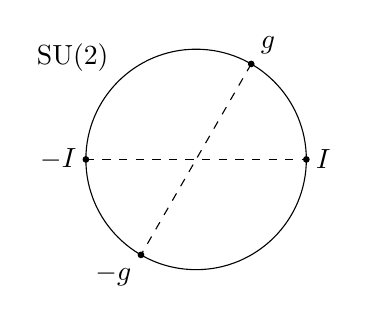
\begin{tikzpicture}[scale=0.7]
      \draw (0,0) circle (2);
      \draw[fill] (2,0) circle (0.05);
      \draw[fill] (-2,0) circle (0.05);
      \node[right] at (2,0) {$I$};
      \node[left] at (-2,0) {$-I$};
      \draw[fill] (1,1.732) circle (0.05);
      \draw[fill] (-1,-1.732) circle (0.05);
      \node[above right] at (1, 1.732) {$g$};
      \node[below left] at (-1, -1.732) {$-g$};
      \draw[dashed] (-2,0)--(2,0);
      \draw[dashed] (1, 1.732)--(-1, -1.732);
      \node[above left] at (-1.414, 1.414) {SU$(2)$};
    \end{tikzpicture}
  \end{center}

  We can in fact explicitly describe exponential map from $\mathfrak{so}(3)$ to SO$(3)$ with the following lemma. 

  \begin{lemma}[Rodrigues' Formula]
    The exponential map $exp: \mathfrak{so}(3) \rightarrow$ SO$(3)$ is defined by 
    \begin{equation}
      e^A = \cos{\theta} I_3 + \frac{\sin{\theta}}{\theta} A + \frac{(1 - \cos{\theta})}{\theta^2} B
    \end{equation}
    where 
    \begin{equation}
      A = \begin{pmatrix}
      0&-c&b\\c&0&-a\\-b&a&0
      \end{pmatrix}, B = \begin{pmatrix}
      a^2&ab&ac\\ab&b^2&bc\\ac&bc&c^2
      \end{pmatrix}
    \end{equation}
    This formula has many applications in kinematics, robotics, and motion interpolation. 
  \end{lemma}

  \begin{theorem}
  The Lie algebras for the following classical Lie groups are summarized as follows. 
  \begin{enumerate}
    \item $\mathfrak{sl}_n \mathbb{R}$ is the real vector space of real $n \times n$ matrices with null trace.
    \item $\mathfrak{so}(n)$ is the real vector space of real $n \times n$ skew-symmetric matrices. 
    \item $\mathfrak{gl}_n \mathbb{R}$ is the real vector space of all real $n \times n$ matrices.
    \item $\mathfrak{o}(n) = \mathfrak{o}(n)$
  \end{enumerate}
  \end{theorem}
  Note that the corresponding groups $\GL(n, \mathbb{R}), \SL(n, \mathbb{R}), \mathfrak{gl}_n \mathbb{R}, \mathfrak{sl}_n \mathbb{R}$ are Lie groups, meaning that they are smooth real manifolds. We can view each of them as smooth real manifolds embedded in the $n^2$ dimensional vector space of real matrices, which is isomorphic to $\mathbb{R}^{n^2}$. 

  \begin{theorem}
    The Lie algebras $\mathfrak{gl}_ \mathbb{R}, \mathfrak{sl}_n \mathbb{R}, \mathfrak{o}(n), \mathfrak{so}(n)$ are well-defined, but only 
    \begin{equation}
      exp: \mathfrak{so}(n) \rightarrow \text{SO}(n)
    \end{equation}
    is surjective. 
  \end{theorem}

  \begin{theorem}
    The Lie algebras for the following classical Lie groups are summarized as follows. 
    \begin{enumerate}
      \item $\mathfrak{sl}_2 \mathbb{C}$ is the real (or complex) vector space of traceless complex $n \times n$ matrices. 
      \item $\mathfrak{u}(n)$ is the real vector space of complex $n \times n$ skew-Hermitian matrices. 
      \item $\mathfrak{su}(n) = \mathfrak{u} \cap \mathfrak{sl}_2 \mathbb{C}$. It is also a real vector space. 
      \item $\mathfrak{gl}_n \mathbb{C}$ is the real (or complex) vector space of complex $n \times n$ matrices. 
    \end{enumerate}
    Note that even though the matrices in these Lie algebras have complex coefficients, we have assigned them to be in a \textbf{real} vector space, which means that we are only allowed to take real linear combinations of these elements. That is, the field we are working over is $\mathbb{R}$ (this does not contradict any of the axioms for vector spaces). For example an element $A$ in $\mathfrak{u}(n)$ or $\mathfrak{su}(n)$ must be anti-self adjoint, but $iA$ is self adjoint. 
  \end{theorem}

  Similarly, the Lie groups 
  \begin{equation}
    \GL(n, \mathbb{C}), \SL(n, \mathbb{C}), \mathfrak{gl}_n \mathbb{C}, \mathfrak{sl}_n \mathbb{C}
  \end{equation}
  are also smooth real manifolds embedded in Mat$(n, \mathbb{C}) \simeq \mathbb{C}^{n^2} \simeq \mathbb{R}^{2 n^2}$. So, we can view these four groups as manifolds embedded in $\mathbb{R}^{2 n^2}$. 

  Note some of the similarities and differences between the real and complex counterparts of these Lie groups and algebras. 
  \begin{enumerate}
    \item $\mathfrak{o}(n) = \mathfrak{so}(n)$, but $\mathfrak{u}(n) \neq \mathfrak{su}(n)$. 
    \item $exp: \mathfrak{gl}_n \mathbb{R} \rightarrow \GL(n, \mathbb{R})$ is not surjective, but $exp: \mathfrak{gl}_n \mathbb{C} \rightarrow \GL(n, \mathbb{C})$ is surjective due to the spectral theorem and surjectivity of $exp: \mathbb{C} \rightarrow \mathbb{C}^*$.
    \item The exponential maps $exp: \mathfrak{u}(n) \rightarrow \text{U}(n)$ and $exp: \mathfrak{su}(n) \rightarrow \text{SU}(n)$ are surjective. 
    \item Still, $exp: \mathfrak{sl}_2 \mathbb{C} \rightarrow \SL(2, \mathbb{C})$ is not surjective. This will be proved now. 
  \end{enumerate}

  \begin{theorem}
    $exp: \mathfrak{sl}_2 \mathbb{C} \rightarrow \SL(2, \mathbb{C})$ is not surjective. 
  \end{theorem}
  \begin{proof}
    Given $M \in \SL(n, \mathbb{C})$, assume that $M = e^A$ for some matrix $A \in \mathfrak{sl}_2 \mathbb{C}$. Putting $A$ into the Jordan Normal Form $J = N A N^{-1}$ means that $J$ can either be of form
    \begin{equation}
      J = \begin{pmatrix}
      0&1\\0&0
      \end{pmatrix}, \begin{pmatrix}
      \lambda&0\\0&-\lambda
      \end{pmatrix} \implies e^J = \begin{pmatrix}
      1&1\\0&1
      \end{pmatrix}, \begin{pmatrix}
      e^\lambda&0\\0&e^{-\lambda}
      \end{pmatrix}
    \end{equation}
    which is also in JNF in $\SL(2, \mathbb{C})$. But a matrix $P \in \SL(2, \mathbb{C})$ may exist with JNF of 
    \begin{equation}
      K = \begin{pmatrix}
      -1&1\\0&-1
      \end{pmatrix}
    \end{equation}
    which is not one of the 2 forms. So, $K \not\in \im{exp} \implies exp$ is not surjective. 
  \end{proof}

  \begin{theorem}
  The exponential maps 
  \begin{align*}
    & exp: \mathfrak{u}(n) \rightarrow \text{U}(n) \\
    & exp: \mathfrak{su}(n) \rightarrow \text{SU}(n)
  \end{align*}
  are surjective. 
  \end{theorem}

\subsubsection{Lie Algebra of SE(n)}

  Recall that the group of affine rigid isometries is denoted SE$(n)$. That is, 
  \begin{equation}
    \text{SE}(n) \equiv \text{SO}(n) \ltimes \text{Tran}\,\mathbb{R}^n
  \end{equation}
  We can define the matrix representation of this affine transformation as such. Given an element $g \in$ SE$(n)$ such that
  \begin{equation}
    g(x) \equiv R x + U, \; R \in \text{SO}(n), U \in \text{Tran}\, \mathbb{R}^n 
  \end{equation}
  we define the representation
  \begin{equation}
    \rho: \text{SE}(n) \rightarrow \GL(n+1, \mathbb{R}), \rho(g) \equiv \begin{pmatrix}
    R&U\\0&1
    \end{pmatrix}
  \end{equation}
  where $R$ is a real $n\times n$ matrix in SO$(n)$ and $U$ is a real $n$-vector in Tran$\,\mathbb{R}^n \simeq \mathbb{R}^n$. We would then have
  \begin{equation}
    \rho(g) \begin{pmatrix}
    x\\1
    \end{pmatrix} \equiv \begin{pmatrix}
    R&U\\0&1
    \end{pmatrix} \begin{pmatrix}
    x\\1
    \end{pmatrix} = \begin{pmatrix}
    R x + U\\1
    \end{pmatrix} \in \mathbb{R}^{n+1}
  \end{equation}

  Clearly, SE$(n)$ is a Lie group, and the matrix representation $\varrho$ of its Lie algebra $\mathfrak{se}(n)$ can be defined as the vector space of $(n+1) \times (n+1)$ matrices of the block form 
  \begin{equation}
    A = \begin{pmatrix}
    \Omega & U \\0 & 0
    \end{pmatrix}
  \end{equation}
  where $\Omega$ is an $n \times n$ skew-symmetric matrix and $U \in \mathbb{R}^n$. Note that there are two different exponential maps here: one belonging to the abstract Lie group SE$(n)$ and another belonging to the concrete, matrix group $\GL(n+1, \mathbb{R})$. This can be represented with the commutative diagram. 
  \[\begin{tikzcd}
  \mathfrak{se}(n) \arrow{r}{exp} \arrow{d}{\varrho} & SE(n) \arrow{d} {\rho}\\
  \mathfrak{gl}_{n+1} \mathbb{R} \arrow{r}{exp} & \GL(n+1, \mathbb{R})
  \end{tikzcd}\]

  \begin{lemma}
    Given any $(n+1) \times (n+1)$ matrix of form 
    \begin{equation}
      A = \begin{pmatrix}
       \Omega & U \\0&0
      \end{pmatrix}
    \end{equation}
    where $\Omega$ is any matrix and $U \in \mathbb{R}^n$, 
    \begin{equation}
      A^k = \begin{pmatrix}
      \Omega^k & \Omega^{k-1} U \\0&0
      \end{pmatrix}
    \end{equation}
    where $\Omega^0 = I_n$, which implies that
    \begin{equation}
      e^A = \begin{pmatrix}
      e^\Omega & V U \\ 0 & 1
      \end{pmatrix}, \; V = I_n + \sum_{k \geq 1} \frac{\Omega^k}{(k+1)!}
    \end{equation}
  \end{lemma}

  \begin{theorem}
    The exponential map
    \begin{equation}
      exp: \mathfrak{se}(n) \rightarrow SE(n)
    \end{equation}
    is well-defined and surjective. 
  \end{theorem}

\subsection{Representations of Lie Groups and Lie Algebras}

  Let $\mathcal{G}$ be an abstract group and let
  \begin{equation}
    \rho: \mathcal{G} \rightarrow \GL(V)
  \end{equation}
  be the representation of $\mathcal{G}$. Then, let $\mathfrak{g}$ be the Lie algebra of $\mathcal{G}$, and $\mathfrak{gl}(V)$ be the Lie algebra of $\GL(V)$. Then, $\rho$ induces another homomorphism 
  \begin{equation}
    \varrho: \mathfrak{g} \rightarrow \mathfrak{gl}(V)
  \end{equation}
  where the bracket structure (in this case, the comutator in the matrix algebra) is preserved. 
  \begin{equation}
    \varrho([X,Y]) = [\varrho(X), \varrho(Y)]
  \end{equation}
  We can visualize this induced homomorphism with the following commutative diagram, which states that $\rho \circ exp = exp \circ \varrho$. 

  \[\begin{tikzcd}
  \mathcal{G} \arrow{r}{\rho} & \GL(V)\\
  \mathfrak{g} \arrow{u}{exp} \arrow{r}{\varrho} & \mathfrak{gl}(V) \arrow{u}{exp}
  \end{tikzcd}\]

  Note that there are very crucial differences between $\rho$ and $\varrho$. First, $\rho$ is a homomorphism between \textbf{groups}, while $\varrho$ is a homomorphism between \textbf{vector spaces}. Additionally, $\GL(V)$ is a group, not a linear space, while $\mathfrak{gl}(V)$ is a linear space. Finally, note that $\GL(V)$ is restricted to only matrices with nonzero determinants, while the elements of $\mathfrak{gl}(V)$ can be any matrix. 

  \begin{example}
    The representation of SE$(n)$ to $\GL(n+1 \mathbb{R}$ and $\mathfrak{se}(n)$ to $\mathfrak{gl}_{n+1} \mathbb{R}$ induces the second homomorphism $\varrho: \mathfrak{gl}_{n+1} \mathbb{R} \rightarrow \GL(n+1, \mathbb{R})$. 
  \end{example}

  \begin{definition}
    The direct sum of representations is a representation. That is, if $U$ is a representation and $V$ is a representation, then $U \oplus V$ is a representation. That is, if 
    \begin{equation}
      \rho_1: \mathcal{G} \rightarrow U, \; \rho_1 (g) = \begin{pmatrix}
      u_1&u_2\\u_3&u_4
      \end{pmatrix}
    \end{equation}
    and
    \begin{equation}
      \rho_2: \mathcal{G} \rightarrow V, \; \rho_2 (g) = \begin{pmatrix}
      v_1 & v_2 \\ v_3 & v_4
      \end{pmatrix}
    \end{equation}
    are two representations of the same group element $g \in \mathcal{G}$, then 
    \begin{equation}
      (\rho_1 \oplus \rho_2): \mathcal{G} \rightarrow (U \oplus V), \;(\rho_1 \oplus \rho_2) (g) = \begin{pmatrix}
      u_1 & u_2 & 0 & 0 \\
      u_3 & u_4 & 0 & 0 \\
      0 & 0 & v_1 & v_2 \\
      0 & 0 & v_3 & v_4 
      \end{pmatrix}
    \end{equation}
    is a bigger representation of $g$ in $U \oplus V$. 
  \end{definition}

  \begin{definition}
    $V$ is irreducible if the only subspaces which are representations are only $V$ and $\{0\}$. 
  \end{definition}

  For our case, we will consider that any representation can be written as a direct sum of irreducible representations. We will now proceed to find an irreducible representation of $\mathfrak{sl}_2 \mathbb{C}$. This means that we want to find the smallest (lowest dimensional) vector space $V$ such that there exists a representation
  \begin{equation}
    \varrho: \mathfrak{sl}_2 \mathbb{C} \rightarrow \mathfrak{gl}(V)
  \end{equation}
  We will write, as shorthand notation, that 
  \begin{equation}
    H = \varrho(H), X = \varrho(X), Y = \varrho(Y)
  \end{equation}
  Clearly, $H, X, Y \in \mathfrak{gl}(V) \simeq \mathfrak{gl}(\mathbb{C}^n)$. By the spectral theorem, we can find an orthonormal basis of eigenvectors $e_1, e_2, ..., e_n$ of the mapping $H$ such that
  \begin{equation}
    H e_i = \lambda_i e_i, \; \lambda_i \in \mathbb{C}
  \end{equation}
  Since $[H,X] = 2X$, it follows that $HX e_i - X H e_i = 2X e_i \implies H (X e_i) = (\lambda_i + 2) (X e_i) \implies Xe_i$ for all $i = 1, 2, ..., n$ are also eigenvectors of $H$ with eigenvalue $(\lambda_i + 2)$, or $X e_i = 0$. So, $X$ is a "ladder operator" that maps each eigenvector $e_i$ with eigenvalue $\lambda_i$ to a different eigenvector $e_j$ with eigenvalue $\lambda_j = \lambda_i + 2$. Having nowhere to be mapped to, the eigenvector with the largest eigenvalue (which must exist since $V$ is finite dimensional) will get mapped to the $0$ vector by $X$. Let us denote this eigenvector having the maximum eigenvalue $m$, as $v_m$. 

  Similarly, $[H,Y] = -2Y$ implies that
  \begin{equation}
    HY e_i - YH e_i = -2Y e_i \implies H(Y e_i) = (\lambda_i - 2)(Y e_i)
  \end{equation}

  implying that $Y$ maps each eigenvector $e_i$ with eigenvaue $\lambda_i$ to another eigenvector $e_j$ with eigenvalue $\lambda_j = \lambda_i - 2$, except for the eigenvector with smallest eigenvalue, which gets mapped to $0$. Since $Y$ clearly maps each eigenvector to a different eigenvector that has a strictly decreasing eigenvalue, we can construct a basis of $V$ to be
  \begin{equation}
    \{v_m, Y v_m, Y^2 v_m, Y^3 v_m, ..., Y^{n-1} v_m\}
  \end{equation}
  (remember that $Y^n v_m = 0$). So, elements of $\mathfrak{sl}_2 \mathbb{C}$ acts on the space $V$ with basis above. To continue, we introduce the following theorem. 

  \begin{theorem}
    \begin{equation}
      X Y^j v_m = j(m-j+1) Y^{j-1} v_m
    \end{equation}
  \end{theorem}
  \begin{proof}
    By induction on $j$ using bracket relations.
  \end{proof}

  $V$ is $n$-dimensional. Since $Y^n v_m = 0$ and $Y^{n-1} v_m \neq 0$, we use the theorem above to get
  \begin{equation}
    0 = X Y^n v_m = n (m-n+1) Y^{n-1} v_m \implies m-n+1=0
  \end{equation}
  So, $n = m+1$, which means that the eigenvalues of $H$ are
  \begin{equation}
    m, m-2, m-4, \ldots, m - 2(n-1) = -m
  \end{equation}

  and we are done. We now classify the 1, 2, and 3 dimensional irreducible representations of $\mathfrak{sl}_2 \mathbb{C}$. 
  \begin{enumerate}
    \item When $n = 1$ (i.e. dimension is 1), $m = n-1 = 0$, meaning that the greatest (and only) eigenvalue is $0$. That is, 
      \begin{equation}
        H v_0 = 0,\; X v_0 = 0,\; Y v_0 = 0
      \end{equation}
    which is the trivial representation of $\mathfrak{sl}_2 \mathbb{C}$. Explicitly, we can completely define the representation (which is a linear homomorphism) with the three equations. 
    \begin{equation}
      \varrho(H) = (0),\; \varrho(X) = (0),\; \varrho(Y) = (0)
    \end{equation}

    \item When $n = 2$ and $m=1$. We now look for a 2 dimensional irreducible representation. The eigenvalues are $1$ and $-1$, with $\{v_1, v_{-1}\}$ as a basis of 2 dimensional space $V$. Then we have 
      \begin{align*}
        & Hv_1 = v_1, \; Hv_{-1} = - v_{-1} \\
        & X v_1 = 0, \; X v_{-1} = v_1 \\
        & Y v_1 = v_{-1}, \; Y v_{-1} = 0
      \end{align*}
    which explicitly translates to the representation $\varrho$ being defined
    \begin{equation}
      \varrho(H) = \begin{pmatrix}
      1&0\\0&-1
      \end{pmatrix}, \; \begin{pmatrix}
      0&1\\0&0
      \end{pmatrix}, \; \begin{pmatrix}
      0&0\\1&0
      \end{pmatrix}
    \end{equation}

    \item When $n=3 \implies m=2$, the basis is $\{v_{-2}, v_0, v_2\}$ with eigenvalues $2, 0, -2$, and the irreducible representation $\varrho$ is defined
      \begin{equation}
        \varrho(H) = \begin{pmatrix}
        2&&\\&0&\\&&-2
        \end{pmatrix}, \varrho(Y) = \begin{pmatrix}
        0&0&0\\1&0&0\\0&1&0
        \end{pmatrix}, \varrho(X) = \begin{pmatrix}
        0&1&0\\0&0&1\\0&0&0
        \end{pmatrix}
      \end{equation}

    \item The same process continues on for $n=4, 5, ...$, and this entirely classifies the irreducible representations of $\mathfrak{sl}_2 \mathbb{C}$. 
  \end{enumerate} 

  \pagebreak

  \subsubsection{Tensor Products of Group Representations}

    \begin{definition}
      If $V$ and $W$ are two different representations of a group $\mathcal{G}$, then we know that $V \oplus W$ is also a representation of $\mathcal{G}$. Furthermore, the tensor product space $V \otimes W$ also defines a representation of $\mathcal{G}$. That is, given representations
      \begin{align*}
        & \rho_V: \mathcal{G} \rightarrow \GL(V) \\
        & \rho_W: \mathcal{G} \rightarrow \GL(W)
      \end{align*}
      The homomorphism $\rho_V \otimes \rho_W: \mathcal{G} \rightarrow \GL(V \otimes W)$ is also a representation of $\mathcal{G}$, which is defined
      \begin{equation}
        (\rho_V \otimes \rho_W)(g) (v \otimes w) \equiv \rho_V (g) (v) \otimes \rho_W (g) (w)
      \end{equation}
      or represented in shorthand notation, 
      \begin{equation}
        g(v \otimes w) \equiv (g v) \otimes (g w)
      \end{equation}
      We know that exp$(H)$ acts on $V$ and $W$ since it is an element of $\GL(V)$ and $\GL(W)$. This means that
      \begin{equation}
        exp(H)(v \otimes w) \equiv \big( exp(H)(v)\big) \otimes \big( exp(H)(w)\big)
      \end{equation}
      If $H$ ($= \rho_V (H)$ or $\rho_W(H)$) has an eigenvalue $\lambda$ on $v$ in $V$ and eigenvalue $\mu$ on $w$ in $W$, then 
      \begin{equation}
        exp(H) (v \otimes w) = (e^\lambda v) \otimes (e^\mu w) = e^{\lambda + \mu} v \otimes w
      \end{equation}
      That is, eigenvalues of $H$ \textbf{add} on tensor products. 
    \end{definition}

    \begin{example}
      Recall that the $2$ dimensional representation $V$ of $\mathfrak{sl}_2 \mathbb{C}$ has eigenvalues $1$ and $-1$ (with corresponding eigenvectors $e_1$ and $e_{-1}$). So, $V \otimes V$ has eigenvalues 
      \begin{align*}
        & (-1) + (-1) = -2, \;\; (-1) + 1 = 0 \\
        & 1 + (-1) = 0, \;\; 1 + 1 = 2
      \end{align*}
      Therefore, the eigenvalues of $V \otimes V$ is $-2$ (geometric multiplicity of 1), $0$ (geometric multiplicity of 2), and $2$ (geometric multiplicity of 1), (Notation-wise, the $n$-dimensional irreducible representation of $\mathfrak{sl}_2 \mathbb{C}$ is denoted $\mathbf{n}$.) which means that
      \begin{equation}
        \mathbf{2} \otimes \mathbf{2} = \mathbf{3} \oplus \mathbf{1}
      \end{equation}
      We can decompose $V \otimes V$ into its symmetric and exterior power components. Sym$^2 V$ has basis (of eigenvectors)
      \begin{equation}
        \{e_{-1} \odot e_{-1}, \; e_{-1} \odot e_1, \; e_1 \odot e_1\}
      \end{equation}
      where the corresponding eigenvalues are $-2$, $0$, and $2$, respectively. So, $\dim{Sym^2 V} = 3$, which means that $Sym^2 V = \mathbf{3}$. As for the exterior power component of $V$, $\Lambda^2 V$ has basis $\{e_{-1} \wedge e_1\}$ with eigenvalue $= 0 \implies \dim{\Lambda^2 V} = 1$, meaning that $\Lambda^2 V = \mathbf{1}$. Therefore, 
      \begin{equation}
        V \otimes V = Sym^2 V \oplus \Lambda^2 V = \mathbf{3} \oplus \mathbf{1}
      \end{equation}
    \end{example}

\subsection{Topological Decompositions of Lie Groups}

  \begin{definition}
    Let us define 
    \begin{enumerate}
      \item S$(n)$ is the vector space of real, symmetric $n \times n$ matrices. 
      \item SP$(n)$ is the set of symmetric, positive semidefinite matrices. 
      \item SPD$(n)$ is the set of symmetric, positive definite matrices. 
    \end{enumerate}
    Note that SP$(n)$ and SPD$(n)$ are not even vector spaces at all. 
  \end{definition}

  \begin{lemma}
    The exponential map 
    \begin{equation}
      exp: S(n) \rightarrow SPD(n)
    \end{equation}
    is a homeomorphism. One may be tempted to call S$(n)$ the Lie algebra of SPD$(n)$, but this is not the case. S$(n)$ is not even a Lie algebra since the commutator is not algebraically closed. Furthermore, SPD$(n)$ is not even a multiplicative group (since matrix multiplication is not closed). 
  \end{lemma}

  Recall from linear algebra the Polar Decomposition. We express this result in a slightly modified way. 

  \begin{theorem}[Polar Decomposition]
    Given a Euclidean space $\mathbb{E}^n$ and any linear endomorphism $f$ of $\mathbb{E}^n$, there are two positive definite self-adjoint linear maps $h_1, h_2 \in$ End$(\mathbb{E}^n)$ and $g \in$ O$(n)$ such that
    \begin{equation}
      f = g \circ h_1 = h_2 \circ g
    \end{equation}
    That is, such that $f$ can be decomposed into the following compositions of functions that commute. 

    \[\begin{tikzcd}
    \mathbb{E}^n \arrow{r}{h_2} & \mathbb{E}^n \\
    \mathbb{E}^n \arrow{u}{g} \arrow{ur}{f} \arrow{r}{h_1} & \mathbb{E}^n \arrow{u}{g}
    \end{tikzcd}\]

    This means that there is a bijection between $Mat(n, \mathbb{R})$ and $O(n) \times SP(n)$. If $f$ is an automorphism, then this decomposition is unique. 
  \end{theorem}

  \begin{corollary}
    The two topological groups are homeomorphic. 
    \begin{equation}
      GL(n, \mathbb{R}) \cong O(n) \times SPD(n)
    \end{equation}
  \end{corollary}

  \begin{corollary}
    For every invertible real matrix $A \in GL(n, \mathbb{R})$, there exists a unique orthogonal matrix $R$ and unique symmetric matrix $S$ such that
    \begin{equation}
      A = R e^S
    \end{equation}
    $\implies$ there is a bijection between $\GL(n, \mathbb{R})$ and $O(n) \times S(n) \simeq \mathbb{R}^{n(n+1)/2}$. Moreover, they are homeomorphic. That is, 
    \begin{equation}
      \GL(n, \mathbb{R}) \simeq O(n) \times S(n) \simeq O(n) \times \mathbb{R}^{n(n+1)/2}
    \end{equation}
    This essentially reduces the study of $\GL(n, \mathbb{R})$ to the study of $O(n)$, which is nice since $O(n)$ is compact. 
  \end{corollary}

  \begin{corollary}
    Given a real matrix $A$, if $\det{A} > 0$, then we can decompose $A$ as
    \begin{equation}
      A = R e^S
    \end{equation}
    where $R \in SO(n)$ and $S \in S(n)$. 
  \end{corollary}

  \begin{corollary}
    There exists a bijection between
    \begin{equation}
      \SL(n, \mathbb{R}) \text{ and } SO(n) \times (S(n) \cap \mathfrak{sl}_n \mathbb{R})
    \end{equation}
  \end{corollary}
  \begin{proof}
    $A \in \SL(n, \mathbb{R}) \implies 1 = \det{A} = \det{R} \det{e^S} = \det{e^S} \implies \det{e^S} = e^{\Tr{S}} = 1 \implies \Tr{S} = 0 \implies S \in$ S$(n) \cap \mathfrak{sl}_n \mathbb{R}$. 
  \end{proof}

  \begin{definition}
    Let us define
    \begin{enumerate}
      \item H$(n)$ is the real vector space of $n \times n$ Hermitian matrices. 
      \item HP$(n)$ is the set of Hermitian, positive semidefinite $n \times n$ matrices. 
      \item HPD$(n)$ is the set of Hermitian, positive definite $n \times n$ matrices. 
    \end{enumerate}
    Similarly, HP$(n)$ and HPD$(n)$ are not vector space. They are just sets. 
  \end{definition}

  \begin{lemma}
    The exponential mapping
    \begin{equation}
      exp: H(n) \rightarrow HPD(n)
    \end{equation}
    is a homeomorphism. 
  \end{lemma}

  However again, HPD$(n)$ is not a Lie group (multiplication is not algebraically closed) nor is H$(n)$ a Lie algebra (commutator is not algebraically closed). By the polar form theorem of complex $n \times n$ matrices, we have a (not necessarily unique) bijection between
  \begin{equation}
    \text{Mat}(n, \mathbb{C}) \text{ and } U(n) \times HP(n)
  \end{equation}
  which implies that
  \begin{equation}
    \GL(n, \mathbb{C}) \cong U(n) \times HPD (n)
  \end{equation}

  \begin{corollary}
    For every complex invertible matrix $A$, there exists a unique decomposition
    \begin{equation}
      A = U e^S
    \end{equation}
    where $U \in U(n)$ and $S \in H(n)$, which implies that the following groups are homeomorphic. 
    \begin{align*}
      \GL(n, \mathbb{C}) & \cong U(n) \times H(n) \\
      & \cong U(n) \times \mathbb{R}^{n^2}
    \end{align*} 
    This essentially reduces the study of $\GL(n, \mathbb{C})$ to that of U$(n)$. 
  \end{corollary}

  \begin{corollary}
    There exists a bijection between 
    \begin{equation}
      \SL(n, \mathbb{C}) \text{ and } SU(n) \times (H(n) \cap \mathfrak{sl}_n \mathbb{C})
    \end{equation}
  \end{corollary}
  \begin{proof}
    Similarly, when $A = U e^S$, we know that $|\det{U}| = 1$ and $\Tr{S}$ is real (since by the Spectral theorem, every self adjoint matrix has a real spectral decomposition). Since $S$ is Hermitian, this implies that $\det{e^S} > 0$. If $A \in \SL(n, \mathbb{C})$, then $\det{A} = 1 \implies \det{e^S} = 1 \implies S \in H(n) \cap \mathfrak{sl}_n \mathbb{C}$. 
  \end{proof}

\subsection{Linear Lie Groups}

  We will assume that the reader has the necessary background knowledge in manifolds, chart mappings, diffeomorphisms, tangent spaces, and transition mappings. 

  Recall that the algebra of real $n \times n$ matrices Mat$(n, \mathbb{R})$ is bijective to $\mathbb{R}^{n^2}$, which is a topological space. Therefore, this bijection 
  \begin{equation}
    i:(\mathbb{R}^{n^2}, \tau_E) \rightarrow \text{Mat}(n, \mathbb{R})
  \end{equation}
  induces a topology on Mat$(n, \mathbb{R})$, defined 
  \begin{equation}
    \tau_M \equiv \{U \in \text{Mat}(n, \mathbb{R}) \; | \; e^{-1} (U) \in \tau_E\}
  \end{equation}
  With this, consider the subset
  \begin{equation}
    \GL(n, \mathbb{R}) \subset \text{Mat}(n, \mathbb{R})
  \end{equation}
  where
  \begin{equation}
    \GL(n, \mathbb{R}) \equiv \{x \in \text{Mat}(n, \mathbb{R}) \;|\; \det{x} \neq 0\}
  \end{equation}
  This set, as we expect, is a multiplicative group. 

  \begin{definition}
    The \textbf{general linear group}, denoted $\GL(n, \mathbb{R})$ is the set of $n \times n$ matrices with nonzero determinant. The more technical definition is that $\GL(n, \mathbb{R})$ is really just the automorphism group of $\mathbb{R}^n$, 
    \begin{equation}
      \GL(n, \mathbb{R}) \equiv \text{Aut}(\mathbb{R}^n)
    \end{equation}
    but it is customary to assume a basis on $\mathbb{R}^n$ in order to realize $\GL(n, \mathbb{R})$ as a matrix group. Note that the procedure of assuming a basis on $\mathbb{R}^n$ is the same as defining a representation of the abstract group $\GL(n, \mathbb{R})$. Both assigns a real $n \times n$ matrix to each element of $\GL(n, \mathbb{R})$. 
  \end{definition}

  In this way, we can view $\GL(n, \mathbb{R})$ as a topological space in $\mathbb{R}^{n^2}$, and it is fine to interpret $\GL(n, \mathbb{R})$ as a matrix group rather than an abstract group. 

  Since the matrix representation of $\GL(n, \mathbb{R})$ is always well defined, the abstract subgroups of $\GL(n, \mathbb{R})$, which are $\SL(n, \mathbb{R}), O(n)$, and $SO(n)$, also have well defined matrix representations (that we are all familiar with). Additionally, since there exists a bijection
  \begin{equation}
    \text{Mat}(n, \mathbb{C}) \cong \mathbb{C}^{n^2} \cong \mathbb{R}^{2 n^2}
  \end{equation}
  we can view $\GL(n, \mathbb{C})$ as a subset of $\mathbb{R}^{2n^2}$, meaning that the subgroups $\SL(n, \mathbb{C}), U(n)$, and $SU(n)$ of $\GL(n, \mathbb{C})$ can also be viewed as subsets of $\mathbb{R}^{2n^2}$. This also applies to $SE(n)$ since it is a subgroup of $\SL(n+1, \mathbb{R})$. We formally state it now. 

  \begin{theorem}
    SE$(n)$ is a linear Lie group. 
  \end{theorem}
  \begin{proof}
    The matrix representation of elements $g \in SE(n)$ is 
    \begin{equation}
      \rho(g) \equiv \begin{pmatrix}
      R_g & U_g \\ 0 & 1
      \end{pmatrix}, \; R_g \in SO(n), U_g \in \mathbb{R}^n
    \end{equation}
    But such matrices also belong to the bigger group $\SL(n+1, \mathbb{R}) \implies SE(n) \subset \SL(n+1, \mathbb{R})$. Moreover, this canonical embedding 
    \begin{equation}
      i: SE(n) \rightarrow \SL(n+1, \mathbb{R})
    \end{equation}
    is a group homomorphism since
    \begin{align*}
      i\big( \rho(g_1 \cdot g_2) \big) & = \begin{pmatrix}
      RS & RV + U \\ 0 & 1
      \end{pmatrix} \\
      & = \begin{pmatrix}
      R & U \\ 0 & 1
      \end{pmatrix} \begin{pmatrix}
      S & V \\ 0 & 1
      \end{pmatrix} = \rho \big( i(g_1) \cdot i(g_2) \big) 
    \end{align*}
    and the inverse is given by 
    \begin{equation}
      \begin{pmatrix}
      R & U \\ 0 & 1
      \end{pmatrix}^{-1} = \begin{pmatrix}
      R^{-1} & - R^{-1} U \\ 0 & 1
      \end{pmatrix} = \begin{pmatrix}
      R^T & - R^T U \\ 0 & 1
      \end{pmatrix}
    \end{equation}
    is also consistent between the inverse operation in SE$(n)$ and $\SL(n+1, \mathbb{R})$. Therefore, SE$(n)$ is a subgroup of $\SL(n+1, \mathbb{R})$, which is a subgroup of $\GL(n+1, \mathbb{R})$. 
  \end{proof}

  Note that even though SE$(n)$ is diffeomorphic (a topological relation) to SO$(n) \times \mathbb{R}^n$, it is \textbf{not} isomorphic (an algebraic relation) sicne group operations are not preserved. Therefore, we write this "equality" as a semidirect product of groups. 
  \begin{equation}
    SE(n) \equiv SO(n) \ltimes \mathbb{R}^n
  \end{equation}

  Therefore, all of the classical Lie groups that we have mentioned can be viewed as subsets of $\mathbb{R}^N$ (with the subspace topology) and as subgroups of $\GL(N, \mathbb{R})$ for some big enough $N$. This defines a special family of Lie groups, called linear Lie groups. 

  \begin{definition}
    A \textbf{linear Lie group} is a subgroup of $\GL(n, \mathbb{R})$ for some $n \geq 1$ which is also a smooth manifold in $\mathbb{R}^{n^2}$. 
  \end{definition}

  \begin{theorem}[Von Neumann, Cartan]
    A closed subgroup $\mathcal{G}$ of $\GL(n, \mathbb{R})$ is a linear Lie group. That is, a closed subgroup $\mathcal{G}$ of $\GL(n, \mathbb{R})$ is a smooth manifold in $\mathbb{R}^{n^2}$.
  \end{theorem}

  \begin{definition}
    Since a linear Lie group $\mathcal{G}$ is a smooth submanifold in $\mathbb{R}^N$, we can take its tangent space at the identity element $I$, which is defined 
    \begin{equation}
      T_I \mathcal{G} \equiv \{p^\prime (0) \;|\; p: I \subset \mathbb{R} \rightarrow \mathcal{G}, p(0) = I\}
    \end{equation}
    where $p$ is a path function on $\mathcal{G}$. 
  \end{definition}

  Note that we haven't mentioned anything about the exponential map up to now. We mention the relationship between this map and the Lie algebra with the following theorem. 

  \begin{theorem}
    Let $\mathcal{G}$ be a linear Lie group. The set $\mathfrak{g}$ defined such that
    \begin{equation}
      \mathfrak{g} \equiv \{X \in \text{Mat}(n, \mathbb{R}) \; | \; e^{t X} \in \mathcal{G} \; \forall t \in \mathbb{R}\}
    \end{equation}
    is equal to the tangent space of $\mathcal{G}$ at the identity element. That is, 
    \begin{equation}
      \mathfrak{g} = T_I \mathcal{G}
    \end{equation}
    Furthermore, $\mathfrak{g}$ is closed under the commutator 
    \begin{equation}
      [A,B] \equiv A B - B A
    \end{equation}
  \end{theorem}

  This theorem ensures that given a linear Lie group $\mathcal{G}$, the tangent space $\mathfrak{g}$ exists and is closed under the commutator. We formally define this space. 

  \begin{definition}
    The Lie algebra of a linear Lie group is a real vector space (of matrices) together with a algebraically closed bilinear map 
    \begin{equation}
      [A,B] \equiv A B - B A
    \end{equation}
    called the \textbf{commutator}. 
  \end{definition} 

  The definition of $\mathfrak{g}$ given in the previous theorem shows that 
  \begin{equation}
    exp: \mathfrak{g} \rightarrow \mathcal{G}
  \end{equation}
  is well defined. In general, exp is neither injective nor surjective. Visually, this exponential mapping is what connects the Lie algebra, i.e. the tangent space of manifold $\mathcal{G}$ to the actual Lie group $\mathcal{G}$. To define the inverse map that maps Lie group elements to Lie algebra ones, we can simply just compute the tangent vectors of the manifold $\mathcal{G}$ at the identity $I$ by taking the derivative of arbitrary path functions in $\mathcal{G}$. That is, for every $X \in T_I \mathcal{G}$, we define the smooth curve 
  \begin{equation}
    \gamma_X: t \mapsto e^{tX}
  \end{equation}
  where $\gamma_X(0) = I$. If we take the derivative of this curve, with respect to $t$ at $t = 0$, we will get the tangent vector $X$ corresponding to that group element $g = e^{X}$. More visually, we just need to take the collection of all smooth path functions $\gamma$ on manifold $\mathcal{G}$ such that $\gamma(0) = I$. Then, taking the derivative of all these paths at $t = 0$ will produce the collection of all tangent vectors at the identity element. We show this process in the following examples. 

  \begin{theorem}
    The matrix representation of $\mathfrak{sl}_n \mathbb{R}$ is precisely the set of traceless $n \times n$ matrices. 
  \end{theorem}

  \begin{proof}
    Clearly, $\mathfrak{sl}_n \mathbb{R}$ is a vector space since it is a Lie algebra. So, $X \in \mathfrak{sl}_n \mathbb{R} \implies t X \in \mathfrak{sl}_n \mathbb{R}$ for all $t \in \mathbb{R} \implies \det{e^{tX}} = 1$ for all $t \in \mathbb{R}$, for all $X \in \mathfrak{sl}_n \mathbb{R}$. But we use the identity 
    \begin{align*}
      \det{e^{tX}} = e^{\Tr{(tX)}} & \implies 1 = e^{\Tr{(t X)}} \\
      & \implies \Tr{(tX)} = 0 \\
      & \implies \Tr{(X)} t = 0 \implies \Tr{X} = 0
    \end{align*}
  \end{proof}
  We now provide an alternative, better proof. We first need a lemma. 

  \begin{lemma}
    $\det^\prime (I) = \Tr$. That is, the differential of the $\det$ operator, evaluated at the identity matrix, is equal to the trace. That is, given any matrix $T$ in the vector space of matrices, 
  \end{lemma}
  \begin{proof}
    \begin{align*}
      \det^\prime (I) (T) = \nabla_T \det(I) \\
      & = \lim_{\varepsilon \rightarrow 0} \frac{\det{(I + \varepsilon T)} - \det{I}}{\varepsilon} \\
      & = \lim_{\varepsilon \rightarrow 0} \frac{\det{(I + \varepsilon T)} - 1}{\varepsilon}
    \end{align*}
    Clearly, $\det(I + \varepsilon(T)) \in \mathbb{R}[\varepsilon]$, where the constant term of the polynomial approaches $1$ and the linear term (coefficient of $\varepsilon$) is $\Tr{T}$. So, 
    \begin{equation}
      \nabla_T \det{I} = \lim_{\varepsilon \rightarrow 0} ... + \Tr{T} = \Tr{T}
    \end{equation}
  \end{proof}

  This means that the instantaneous rate at which $\det$ changes at $I$ when traveling in direction $T$ is directly proportional to $\Tr{T}$. Now, we provide an alternative proof of the theorem. 
  \begin{proof}
    Let $R: \mathbb{R} \rightarrow \SL(n, \mathbb{R})$ such that $R(0) = I$. Then, by definition, $\im{R} \subset \SL(n, \mathbb{R}) \implies \det{(R(t))} = 1$ for all $t \in (-\varepsilon, \varepsilon)$. Compute the derivative of the mapping $\det \circ R$. 
    \begin{align*}
        (\det \circ  R) (t) = 1 & \implies \det^\prime \big( R(t) \big) \cdot R^\prime (t) \\ 
        & \implies \det^\prime (I) = \det^\prime \big(R(t)\big) = 0 
    \end{align*}
    We now use the previous lemma get that 
    \begin{equation}
      \det^\prime \big( R^\prime(0)\big) = \det^\prime (I)=0 \implies \Tr{R^\prime(0)} = 0
    \end{equation}
  \end{proof} 

  \begin{theorem}
    The matrix representation of $\mathfrak{so}(n)$ is precisely the set of antisymmetric matrices. 
  \end{theorem}
  \begin{proof}
    Let $R: \mathbb{R} \rightarrow SO(n)$ be a arbitrary smooth curve in $\SL(n)$ such that $R(0) = I$. Then, for all $t \in (-\epsilon, \epsilon)$, 
    \begin{equation}
      R(t) R(t)^T = I
    \end{equation}
    Taking the derivative at $t = 0$, we get
    \begin{equation}
      R^\prime (0) R(0)^T + R(0) R^\prime(0)^T = 0 \implies R^\prime (0) + R^\prime(0)^T = 0
    \end{equation}
    which states that the tangent vector $X = R^\prime (0)$ is skew symmetric. Since the diagonal elements of a skew symmetric matrix are $0$, the trace is $0$ and the condition that $\det{R} = 1$ yields nothing new. This shows that $\mathfrak{o}(n) = \mathfrak{so}(n)$. 
  \end{proof}




  We have only worked with linear Lie groups so far. The reason that linear Lie groups are so nice to work with is because they have well defined matrix representations. This allows us to have concrete structures on these groups and their Lie algebras. 
  \begin{enumerate}
    \item A linear Lie group is concretely defined as a submanifold of $\mathbb{R}^N$, while a general one is an abstract manifold. 
    \item The Lie bracket with regards to a linear Lie group is defined to be the commutator 
      \begin{equation}
        [A,B] \equiv A B - B A
      \end{equation}
    but for elements that are not matrices this doesn't make sense. 

    \item The exponential map from the algebra to the group is defined
      \begin{equation}
        e^A \equiv \sum_{k=0}^\infty \frac{1}{k!} A^k
      \end{equation}
    but if $A$ is not a matrix, then exp cannot be defined this way.
  \end{enumerate}
  We seek to generalize these concepts to abstract Lie groups, but we will do this in the next section. 

  \subsubsection{Lie Algebras of SO(3) and SU(2), Revisited}

    \begin{example}
      The Lie algebra $\mathfrak{so}(3)$ is the real vector space of $3 \times 3$ skew symmetric matrices of form 
      \begin{equation}
        \begin{pmatrix}
        0 & -d & c \\ d & 0 & -b \\ -c & b & 0
        \end{pmatrix}
      \end{equation}
      where $b, c, d \in \mathbb{R}$. The Lie bracket $[A,B]$ of $\mathfrak{so}(3)$ is also just the usual commutator. 

      We can define an isomorphism of Lie algebras $\psi: (\mathbb{R}^3, \times) \rightarrow \mathfrak{so}(3)$ (where $\times$ is the cross product) by the formula 
      \begin{equation}
        \psi(b, c, d) \equiv \begin{pmatrix}
        0 & -d & c \\
        d & 0 & -b \\
        -c & b & 0
        \end{pmatrix}
      \end{equation}
      where, by definition, 
      \begin{equation}
        \psi(u \times v) = [\psi(u), \psi(v)]
      \end{equation}
      It is also easily verified that for all $u, v \in \mathbb{R}^3$, 
      \begin{equation}
        \psi(u) (v) = u \times v
      \end{equation}
    \end{example}

    \begin{example}
      Similarly, we can see that $\mathfrak{su}(2)$ is the real vector space consisting of all complex $2 \times 2$ skew Hermitian matrices of null trace, which is of form
      \begin{equation}
        i(d \sigma_1 + c \sigma_2 + b \sigma_3) = \begin{pmatrix}
        i b & c + i d\\
        -c + i d & - i b
        \end{pmatrix}
      \end{equation}
      where $\sigma_1, \sigma_2, \sigma_3$ are the Pauli spin matrices. We can also define an isomorphism of Lie algebras $\varphi: (\mathbb{R}^3, \times) \rightarrow \mathfrak{su}(2)$ by the formula
      \begin{equation}
        \varphi(b, c, d) = \frac{i}{2} (d \sigma_1 + c \sigma_2 + b \sigma_3) = \frac{1}{2} \begin{pmatrix}
        i b & c + i d\\
        -c + i d & - i b
        \end{pmatrix}
      \end{equation}
      where, by definition of ismorphism, we have
      \begin{equation}
        \varphi(u \times v) = [\varphi(u), \varphi(v)]
      \end{equation}
    \end{example}

    We now restate the connection between the groups SO$(3)$ and SU$(2)$. Note that letting $\theta = \sqrt{b^2 + c^2 + d^2}$, we can write 
    \begin{equation}
      A = \frac{1}{\theta} (d \sigma_1 + c \sigma_2 + b \sigma_3) = \frac{1}{\theta} \begin{pmatrix}
      i b & c + i d\\
      -c + i d & - i b
      \end{pmatrix}
    \end{equation}
    such that $A^2 = I$. With this, we can rewrite the exponential map as 
    \begin{equation}
      exp: \mathfrak{su}(2) \rightarrow SU(2), \; exp(i \theta A) = \cos{\theta} I  + i \sin{\theta} A
    \end{equation}
    As for the isomorphism $\varphi: (\mathbb{R}^3, \times) \rightarrow \mathfrak{su}(2)$, we have
    \begin{equation}
      \varphi(b, c, d) \equiv \frac{1}{2} \begin{pmatrix}
      i b & c + i d\\
      -c + i d & - i b
      \end{pmatrix} = i \frac{\theta}{2} A
    \end{equation}
    Similarly, we can view the exponential map $exp: (\mathbb{R}^3, \times) \rightarrow SU(2)$ as 
    \begin{equation}
      exp(\theta v) = 
    \end{equation}


    \begin{example}
      The lie algebra $\mathfrak{se}(n)$ is the set of all matrices of form 
      \begin{equation}
        \begin{pmatrix}
        B & U \\ 0 & 0
        \end{pmatrix}
      \end{equation}
      where $B \in \mathfrak{so}(n)$ and $U \in \mathbb{R}^n$. The Lie bracket is given by
      \begin{equation}
        \begin{pmatrix}
        B & U \\ 0 & 0
        \end{pmatrix} \begin{pmatrix}
        C & V \\ 0 & 0
        \end{pmatrix} - \begin{pmatrix}
        C & V \\ 0 & 0
        \end{pmatrix} \begin{pmatrix}
        B & U \\ 0 & 0
        \end{pmatrix} = \begin{pmatrix}
        BC - CB & BV - CU \\ 0 & 0
        \end{pmatrix}
      \end{equation}
    \end{example}

\subsection{Abstract Lie Groups}

  \begin{definition}
    A (real) \textbf{Lie group} $\mathcal{G}$ is a group $\mathcal{G}$ that is also a real, finite-dimensional smooth manifold where  group multiplication and inversion are smooth maps. 
  \end{definition}

  \begin{definition}
    A (real) Lie algebra $\mathfrak{g}$ is a real vector space with a map 
    \begin{equation}
      [\cdot, \cdot]: \mathfrak{g} \times \mathfrak{g} \rightarrow \mathfrak{g}
    \end{equation}
    called the Lie bracket satisfying bilinearity, antisymmetricity, and the Jacobi Identity. 
  \end{definition}

  To every Lie group $\mathcal{G}$ we can associate a Lie algebra $\mathfrak{g}$ whose underlying vector space is the tangent space of $\mathcal{G}$ at the identity element. Additionally, the exponential map allows us to map elements from the Lie algebra to the Lie group. These concrete definitions in the context of linear Lie groups is easy to work with, but has some minor problems: to use it we first need to represent a Lie group as a group of matrices, but not all Lie groups can be represented in this way. 

  To do this, we must introduce further definitions. 

  \begin{definition}
    Let $M_1$ ($m_1$-dimensional) and $M_2$ ($m_2$ dimensional) be manifolds in $\mathbb{R}^N$. For any smooth function $f: M_1 \rightarrow M_2$ and any $p \in M_1$, the function 
    \begin{equation}
      f^\prime_p: T_p M_1 \rightarrow T_{f(p)} M_2
    \end{equation}
    called the \textbf{tangent map, derivative, or differential} of $f$ at $p$, is defined as follows. For every $v \in T_p M_1$ and every smooth curve $\gamma: I \rightarrow M_1$ such that $\gamma(0) = p$ and $\gamma^\prime (0) = v$ , 
    \begin{equation}
      f^\prime_p(v) \equiv (f \circ \gamma)^\prime (0)
    \end{equation}
    The map $f^\prime_p$ is also denoted $d f_p$ and is a linear map. 
  \end{definition}

  \begin{definition}
    Given two Lie groups $\mathcal{G}_1$ and $\mathcal{G}_2$, a \textbf{homomorphism of Lie groups} is a function 
    \begin{equation}
      f: \mathcal{G}_1 \rightarrow \mathcal{G}_2
    \end{equation}
    that is both a group homomorphism and a smooth map (between manifolds $\mathcal{G}_1$ and $\mathcal{G}_2$). An \textbf{isomorphism of Lie groups} is a bijective function $f$ such that both $f$ and $f^{-1}$ are homomorphisms of Lie groups. 
  \end{definition}

  \begin{definition}
    Given two Lie algebras $\mathfrak{g}_1$ and $\mathfrak{g}_2$, a \textbf{homomorphism of Lie algebras} is a function 
    \begin{equation}
      f: \mathfrak{g}_1 \rightarrow \mathfrak{g}_2
    \end{equation}
    that is a linear homomorphism that preserves Lie brackets; that is, 
    \begin{equation}
      f([A,B]) = [f(A), f(B)]
    \end{equation}
    for all $A, B \in \mathfrak{g}$. An \textbf{isomorphism of Lie algebras} is a bijective function $f$such that both $f$ and $f^{-1}$ are homomorphisms of Lie algebras. 
  \end{definition}

  \begin{theorem}
    If $f: \mathcal{G}_1 \rightarrow \mathcal{G}_2$ is a homomorphism of Lie groups, then 
    \begin{equation}
      f_I^\prime: \mathfrak{g}_1 \rightarrow \mathfrak{g}_2
    \end{equation}
    is a homomorphism of Lie algebras. 
  \end{theorem}

  We have explained how to construct the Lie bracket (as the commutator) of the Lie algebra of a linear Lie group, but we have not defined how to construct the Lie bracket for general Lie groups. There are several ways to do this, and we describe one such way through \textbf{adjoint representations}. 

  \begin{definition}
    Given a Lie group $\mathcal{G}$, we define a \textbf{left translation} as the map
    \begin{equation}
      L_a: \mathcal{G} \rightarrow \mathcal{G}, \; L_a (b) \equiv a b
    \end{equation}
    for all $b \in \mathcal{G}$. Similarly, the \textbf{right translation} is defined
    \begin{equation}
      R_a: \mathcal{G} \rightarrow \mathcal{G}, \; R_a (b) \equiv b a
    \end{equation}
    for all $b \in \mathcal{G}$. 
  \end{definition}

  Both $L_a$ and $R_a$ are diffeomorphisms. Additionally, given the automorphism
  \begin{equation}
    R_{a^{-1}} L_a \equiv R_{a^{-1}} \circ L_a, \; R_{a^{-1}} L_a (b) \equiv a b a^{-1}
  \end{equation}
  the derivative
  \begin{equation}
    (R_{a^{-1}} L_a)^\prime_I: \mathfrak{g} \rightarrow \mathfrak{g}
  \end{equation}
  is an ismorphism of Lie algebras, also denoted 
  \begin{equation}
    \text{Ad}_a: \mathfrak{g} \rightarrow \mathfrak{g}
  \end{equation}

  \begin{definition}
    This induces another map $a \mapsto$ Ad$_a$, which is a map of Lie groups
    \begin{equation}
      Ad: \mathcal{G} \rightarrow \GL(\mathcal{\mathfrak{g}})
    \end{equation}
    which is called the \textbf{adjoint representation of $\mathcal{G}$}. In the case of a linear map, we can verify that 
    \begin{equation}
      \text{Ad}(a) (X) \equiv \text{Ad}_a (X) \equiv a X a^{-1}
    \end{equation}
    for all $a \in \mathcal{G}$ and for all $X \in \mathfrak{g}$. 
  \end{definition}

  \begin{definition}
    Furthermore, the derivative of this map at the identity 
    \begin{equation}
      \text{Ad}_I^\prime: \mathfrak{g} \rightarrow \mathfrak{gl}(\mathfrak{g})
    \end{equation}
    is a map between Lie algebras, denoted simply as 
    \begin{equation}
      \text{ad}: \mathfrak{g} \rightarrow \mathfrak{gl}(\mathfrak{g})
    \end{equation}
    called the \textbf{adjoint representation} of $\mathfrak{g}$. It is easily visualized with the following commutative diagram. 

    \[\begin{tikzcd}
    \mathcal{G} \arrow{r}{Ad} & \GL(\mathfrak{g}) \\
    \mathfrak{g} \arrow{u}{exp} \arrow{r}{ad} & \mathfrak{gl}(\mathfrak{g}) \arrow{u}{exp}
    \end{tikzcd}\]

    We define the map ad to be 
    \begin{equation}
      ad(A)(B) \equiv [A,B]
    \end{equation}
    where $[A,B]$ is the Lie bracket (of $\mathfrak{g}$) of $A, B \in \mathfrak{g}$. We can actually conclude something stronger about this mapping. Since the Lie bracket of $\mathfrak{g}$ satisfies the properties of the bracket, the Jacobi identity of $[\cdot, \cdot]$ implies that ad is a Lie algebra homomorphism. 
    \begin{align*}
      & [x, [y,z]] + [y,[z,x]] + [z, [x,y]] = 0 \\
      \implies & [x, ad(y)(z)] + [y, ad(z)(x)] + [z, ad(x)(y)] = 0 \\
      \implies & ad(x)\big(ad(y)(z)\big) + ad(y) \big( ad(z)(x)\big) + ad(z) \big(ad(x)(y)\big) = 0 \\
      \implies & ad(x) ad(y) (z) - ad(y) ad(x) z - ad \big(ad(x)(y)\big) (z) = 0 \\
      \implies & \big( ad(x) ad(y) - ad(y) ad(x) \big) (z) = ad\big( ad(x)(y) \big) (z) \\
      \implies & [ad(x), ad(y)] (z) = ad ([x,y]) (z) \\
      \implies & [ad(x), ad(y)] = ad([x,y])
    \end{align*}
    Therefore, ad preserves brackets and thus ad is a Lie algebra homomorphism. That is, 
    \begin{equation}
      \text{ad}([A,B]) = [\text{ad}(A), \text{ad}(B)]
    \end{equation}
    Note that the bracket on the left side represents the bracket of $\mathfrak{g}$, while the bracket on the right represents the Lie bracket from the Lie algebra $\mathfrak{gl}(\mathfrak{g})$. The fact that ad is a Lie algebra homomorphism indicates that it is a representation of $\mathfrak{g}$, which is why it's called the adjoint representation. 
  \end{definition}

  \begin{definition}
    This construction finally allows us to define the Lie bracket in the case of a general Lie group. The Lie bracket on $\mathfrak{g}$ is defined as 
    \begin{equation}
      [A,B] \equiv \text{ad} (A) (B)
    \end{equation}
  \end{definition}

  We would also need to introduce a general exponential map for non-linear Lie groups, but we will not do it here. 


\section{Exercises} 

\subsection{Group Like Structures}

  \begin{exercise}[Math 401 Spring 2025 Midterm 2]
    Listed. 
    \begin{enumerate}
      \item Let $G$ be a finite group with an even number of elements. Show that $G$ contains an element of order $2$. 
      \item Prove that a group of order $10$ contains an element of order $5$. 
    \end{enumerate}
  \end{exercise}
  \begin{solution}
    Listed. 
    \begin{enumerate}
      \item We know that $e^{-1} = e$, and so remove it from $G$. Then $G$ has an odd number of elements. Now as long as $G$ is nonempty, we can remove $a, a^{-1}$, resulting in an odd cardinality. Since $G$ is finite, this must terminate, and so there must be a case where $a = a^{-1} \implies \ord(a) = 2$. 
      \item Assume that there is no element of order $5$. Then from above it must contain an element of order $2$, and let us call it $a \in G$. $\ord(e) = 1$ obviously. If any $b \in G$ had order 10, then $G = Z_{10}$, which would mean that $\ord(b^5) = 2$. Therefore every element other than the identity must have order $2$. But then given $a, b, ab \in G$, $ab \neq a, b$ since $ab = a \implies b = e$, and this is precisely the Klein 4 group. This subgroup has an order that doesn't divide 10, contradicting Lagrange's theorem. 
    \end{enumerate}
  \end{solution}

  \begin{exercise}[Shifrin 6.1.1]
    Which of the following are groups?
    \begin{enumerate}
      \item[(a)] $\{1,3,7,9\} \subset \mathbb{Z}_{10}$, with operation multiplication
      \item[(b)] $\{0,2,4,6\} \subset \mathbb{Z}_{10}$, with operation addition
      \item[(c)] $\{x \in \mathbb{Q} : 0 < x \leq 1\}$, with operation multiplication
      \item[(d)] the set of all positive irrational real numbers, with operation multiplication
      \item[(e)] the set of imaginary numbers $ix, x \in \mathbb{R}$, with operation addition
      \item[(f)] the set of complex numbers of modulus 1, with operation multiplication
      \item[(g)] $\mathbb{Z}$ with operation $a \bullet b = a + b + 1$
      \item[(h)] $\mathbb{Z}$ with operation $a \bullet b = a - b$
      \item[(i)] $\mathbb{Q} - \{1\}$ with operation $a \bullet b = a + b - ab$
    \end{enumerate}
  \end{exercise}
  \begin{solution}
    Listed. We will denote the sets in question to be $G$. 
    \begin{enumerate}
      \item[(a)] Is a group since product of 2 odds is odd, so is closed. Also we have $1$ as the identity with $3^{-1} = 7, 7^{-1} = 3, 9^{-1} = 9$. It is associative since multiplication on $\mathbb{Z}_{10}$ is associative. 
      \item[(b)] Not a group since $4 + 4 = 8 \not\in G$. 
      \item[(c)] Not a group since $1/2 \in G$ but $(1/2)^{-1} = 2 \not\in G$. 
      \item[(d)] Not a group since $\sqrt{2} \times \sqrt{2} 2  \not\in G$. 
      \item[(e)] Is a group since identity is $0 = 0i$, $ix + iy = i (x + y)$ with $x + y \in \mathbb{R}$, and $-(ix) = i (-x)$ where $-x \in \mathbb{R}$. 
      \item[(f)] Is a group since this is a representation of $O(2)$. 
      \item[(g)] Is a group since this is obviously closed under $\mathbb{Z}$ since $+_{\mathbb{Z}}$ is closed. Now assume that $i$ is the identity. Then $a \bullet i = a + i + 1 = a \implies i = -1$. Therefore $a \bullet a^{-1} = a + a^{-1} + 1 = -1 \implies a^{-1} = -a - 2$. This is associative since 
      \begin{equation}
        (a \bullet b) \bullet c = (a + b + 1) \bullet c = a + b + c + 2 = a \bullet (b + c + 1) = a \bullet (b \bullet c)
      \end{equation}
      \item[(h)] Not a group since it is not associative. Note $(a \bullet b) \bullet c = (a - b) \bullet c = a - b - c$, while $a \bullet (b \bullet c) = a \bullet (b - c) = a - b + c$. 
      \item[(i)] Is a group. We claim that it is closed. Assume not; given $a, b \neq 1$, 
        \begin{equation}
          a \bullet b = a + b - ab = 1 \implies 0 = ab - a - b + 1 = (a - 1)(b-1) 
        \end{equation}
        which means $a = 1$ or $b = 1$, which is a contradiction. As for the identity, $a \bullet i = a + i - ai = a \implies 0 = i - ai = i (1 - a) \implies i = 0$ since $a \neq 1$. We can define the inverse by solving 
        \begin{equation}
          0 = a \bullet a^{-1} = a + a^{-1} - a a^{-1} \implies a^{-1} (1 - a) = -a \implies a^{-1} = \frac{a}{a-1}
        \end{equation}
        which is well-defined since $a \neq 1$. Finally, it is associative since 
        \begin{align}
          (a \bullet b) \bullet c & = (a + b - ab) \bullet c \\
                                  & = a + b - ab + c - ac - bc - abc \\
                                  & = a + b + c - bc - ab - ac - abc \\
                                  & = a \bullet (b + c - bc) \\
                                  & = a \bullet (b \bullet c)
        \end{align}
    \end{enumerate}
  \end{solution}

  \begin{exercise}[Shifrin 6.1.10]
    \begin{enumerate}
      \item[(a)] Let $G$ be a group. Prove that $(ab)^2 = a^2b^2$ for all $a,b \in G$ if and only if $G$ is abelian.
      \item[(b)] Prove that if every element (other than the identity element) of a group $G$ has order 2, then $G$ is abelian.
    \end{enumerate}
  \end{exercise}
  \begin{solution}
    For (a), if $G$ is abelian, then 
    \begin{equation}
      (ab)^2 = (ab) (ab) = a (ba) b = a (ab) b = (aa) (bb) = a^2 b^2
    \end{equation}
    If the identity holds, then 
    \begin{equation}
      (ab)^2 = a^2 b^2 \implies (a^{-1} a) (ba) (b b^{-1}) = a^{-1} (ab)(ab) b^{-1} = a^{-1} a^2 b^2 b^{-1} \implies ba = ab
    \end{equation} 
    For (b), since we have $a^2 = e, b^2 = e$, and $(ab)^2 = e$, from (a) $G$ is abelian. 
  \end{solution}

  \begin{exercise}[Shifrin 6.1.17]
    \begin{enumerate}
      \item[(a)] A group has four elements $a$, $b$, $c$, and $d$, subject to the rules $ca = a$ and $d^2 = a$. Fill in the entire multiplication table at the left below.
      
      \begin{tabular}{c|cccc}
        $\cdot$ & $a$ & $b$ & $c$ & $d$ \\
        \hline
        $a$ & & & & \\
        $b$ & & & & \\
        $c$ & $a$ & & & \\
        $d$ & & & & $a$ \\
      \end{tabular}
      
      \item[(b)] A group has six elements $a$, $b$, $c$, $d$, $e$, and $f$, subject to the rules $ae = a$, $bd = a$, $c^2 = a$, and $df = a$. Fill in the entire multiplication table at the right above.
      
      \begin{tabular}{c|cccccc}
        $\cdot$ & $a$ & $b$ & $c$ & $d$ & $e$ & $f$ \\
        \hline
        $a$ & & & & & $a$ & \\
        $b$ & & & & $a$ & & \\
        $c$ & & & $a$ & & & \\
        $d$ & & & & & & $a$ \\
        $e$ & & & & & & \\
        $f$ & & & & & & \\
      \end{tabular}
    \end{enumerate}
  \end{exercise}
  \begin{solution}
    We can see that $ca = a \implies c = ca a^{-1} = a a^{-1} = i$, so $c$ is the identity. We can fill in the row and column of $c$. Then, we can figure out what $bd$ is. It cannot be $b$ or $d$ since $c$ is the unique identity, so it must be either $a$ or $c$. It cannot be $a$ since then $bd = a = d^2$, and so $b = d$. So it must be $c$. By the same logic we can fill out the rest of the rows and columns. 

    \begin{tabular}{c|cccc}
      $\cdot$ & $a$ & $b$ & $c$ & $d$ \\
      \hline
      $a$ & $c$ & $d$ & $a$ & $b$ \\
      $b$ & $d$ & $a$ & $b$ & $c$ \\
      $c$ & $a$ & $b$ & $c$ & $d$ \\
      $d$ & $b$ & $c$ & $d$ & $a$ \\
    \end{tabular}

    By the same logic as the previous, we can immediately see that $ae = a \implies e$ is the identity. The formal logic above can be simplified down to saying that there can be no two of the same elements in the same row or column, since if it were, then we are saying that $xy = xz \implies y = z$, which cannot be the case since $y$ and $z$ are distinct. So $fb = a$. We can also deduce that $da = ab$ and $ba = af$. At this point, we can recognize that this is the Dihedral group of order $6$, and so we fill in the rest of the multiplication table. 

    \begin{tabular}{c|cccccc}
      $\cdot$ & $a$ & $b$ & $c$ & $d$ & $e$ & $f$ \\
      \hline
      $a$ & c & f & e & b & a & d \\
      $b$ & d & e & f & a & b & c \\
      $c$ & e & d & a & f & c & b \\
      $d$ & f & c & b & e & d & a \\
      $e$ & a & b & c & d & e & f \\
      $f$ & b & a & d & c & f & e
    \end{tabular}
  \end{solution}

\subsection{Subgroups and Quotient Groups}

  \begin{exercise}[Shifrin 6.2.2]
    Prove that $\mathbb{Z}_7^{\times} \cong \mathbb{Z}_6$. (It is crucial to remember that we multiply in $\mathbb{Z}_7^{\times}$ and add in $\mathbb{Z}_6$.)
  \end{exercise}
  \begin{solution}
    Both groups are of order 6, and so $\mathbb{Z}_7^\times$---which is indeed a group (since it is the group of units of the ring $(\mathbb{Z}_7, +, \times)$)---must be isomorphic to either $\mathbb{Z}_6$ or $S_3$. However, $S_3$ is not abelian, while $\mathbb{Z}^\times_7$ is, so it must be the case that it is isomorphic to $\mathbb{Z}_6$. 
  \end{solution}

  \begin{exercise}[Shifrin 6.2.15.a/b]
    The \textbf{dihedral group} of order $2n$, denoted $\mathcal{D}_n$, is given by $\{\rho^i\psi^j : 0 \leq i < n, 0 \leq j \leq 1\}$ subject to the rules $\rho^n = e$, $\psi^2 = e$, and $\psi\rho\psi^{-1} = \rho^{-1}$.
    \begin{enumerate}
      \item Check this is really a group. That is, what is $(\rho^i\psi^j)^{-1}$, and what is the product $(\rho^i\psi^j)(\rho^k\psi^\ell)$?
      \item Check that $\mathcal{T} \cong \mathcal{D}_3$ and $S_q \cong \mathcal{D}_4$.
    \end{enumerate}
  \end{exercise}
  \begin{solution}
    We check the properties of a group. The following identity is useful: 
    \begin{equation}
      (\psi \rho \psi^{-1})^{n-i} = (\rho^{-1})^{n-i} \implies \psi \rho^{n-i} \psi^{-1} = \rho^i \implies \psi \rho^{n-i} = \rho^i \psi
    \end{equation}
    \begin{enumerate}
      \item \textit{Closure}. From simplifying according to the first two rules, we will automatically adjust the exponents to be $i, k < n$ (by subtracting out multiples of $n$) and $j \in \{0, 1\}$ (by subtracting out multiples of $2$). Going case by case, 
      \begin{enumerate}
        \item $j = 0, l = 0$. $\rho^i \rho^k = \rho^{i+k}$. 
        \item $j = 0, l = 1$. $\rho^i \rho^k \psi = \rho^{i+k} \psi$. 
        \item $j = 1, l = 0$. $\rho^i \psi \rho^k = \rho^i \rho^{n-k} \psi = \rho^{n-k+i} \psi$. 
        \item $j = 1, l = 1$. $\rho^i \psi \rho^k \psi = \rho^i \psi \psi \rho^{n-k} = \rho^i \rho^{n-k} = \rho^{n-k+i}$. 
      \end{enumerate}
      \item \textit{Identity}. The identity is $e = \rho^0 \psi^0$. We can see that $e \rho^i \psi^j = \rho^i \psi^j e = \rho^{i+0} \psi^j$. 
      \item \textit{Inverse}. We have $\psi \rho \psi^{-1} = \psi \rho \psi = \rho^{-1} \implies \psi \rho = \rho^{-1} \psi^{-1} = (\psi \rho)^{-1}$. Therefore, 
      \begin{equation}
        (\rho^i \psi^j)^{-1} = \begin{cases} 
          \rho^{n - i} & \text{ if } j = 0  \\
          \rho^{i} \psi & \text{ if } j = 1
        \end{cases}
      \end{equation}
      which are both of the correct form and therefore in $\mathcal{D}_n$. To verify, we see that $\rho^i \rho^{n-i} = \rho^n = e$, and $(\rho^i \psi) (\rho^i \psi) = \rho^i \psi \psi \rho^{n-i} = \rho^i \rho^{n-i} = e$.  
      \item \textit{Associativity}. Can also be proven tediously but problem only asked to state the product and inverse.  
    \end{enumerate} 

    For (b) for $\mathcal{T}$, we can explicitly look at the multiplication tables and see that they are isomorphic. We denote $r_1, r_2$ as the 120 and 240 degree rotations, and $f_1, f_2, f_3$ as the flips across each axis. 

    \begin{figure}[H]
      \centering
      \begin{subfigure}[b]{0.48\textwidth}
        \centering
        \begin{tabular}{c|cccccc}
          & $e$ & $\rho$ & $\rho^2$ & $\psi$ & $\rho\psi$ & $\rho^2\psi$ \\
          \hline
          $e$ & $e$ & $\rho$ & $\rho^2$ & $\psi$ & $\rho\psi$ & $\rho^2\psi$ \\
          $\rho$ & $\rho$ & $\rho^2$ & $e$ & $\rho^2\psi$ & $\psi$ & $\rho\psi$ \\
          $\rho^2$ & $\rho^2$ & $e$ & $\rho$ & $\rho\psi$ & $\rho^2\psi$ & $\psi$ \\
          $\psi$ & $\psi$ & $\rho^2\psi$ & $\rho\psi$ & $e$ & $\rho^2$ & $\rho$ \\
          $\rho\psi$ & $\rho\psi$ & $\psi$ & $\rho^2\psi$ & $\rho$ & $e$ & $\rho^2$ \\
          $\rho^2\psi$ & $\rho^2\psi$ & $\rho\psi$ & $\psi$ & $\rho^2$ & $\rho$ & $e$
        \end{tabular}
        \caption{$\mathcal{D}_3$}
      \end{subfigure}
      \hfill 
      \begin{subfigure}[b]{0.48\textwidth}
        \centering
        \begin{tabular}{c|cccccc}
          & $e$ & $r_1$ & $r_2$ & $f_1$ & $f_2$ & $f_3$ \\
          \hline
          $e$ & $e$ & $r_1$ & $r_2$ & $f_1$ & $f_2$ & $f_3$ \\
          $r_1$ & $r_1$ & $r_2$ & $e$ & $f_3$ & $f_1$ & $f_2$ \\
          $r_2$ & $r_2$ & $e$ & $r_1$ & $f_2$ & $f_3$ & $f_1$ \\
          $f_1$ & $f_1$ & $f_2$ & $f_3$ & $e$ & $r_2$ & $r_1$ \\
          $f_2$ & $f_2$ & $f_3$ & $f_1$ & $r_1$ & $e$ & $r_2$ \\
          $f_3$ & $f_3$ & $f_1$ & $f_2$ & $r_2$ & $r_1$ & $e$
        \end{tabular}
        \caption{$\mathcal{T}$}
      \end{subfigure}
    \end{figure}

    For $S_q$, it is tedious to write the full table, so we construct the isormorphisms using the generators. For $S_q$, the symmetry group of the square consists of 8 elements: the 4 rotations $r_1, r_2, r_3, r_4$ (of 90, 180, 270, and 360=0 degrees), and the flips $f_1, f_2, f_3, f_4$ (across each axis). Now we construct the function $g: \mathcal{D}_3 \rightarrow \mathcal{T}$ such that $f(\rho) = r_1$ and $f(\psi) = f_1$. Then we can see that 
    \begin{equation}
      g(\rho^4) = g(e) = e = r_1^4 = g(\rho^4), \qquad g(\psi^2) = g(e) = e = f_1^2 = g(\psi)^2
    \end{equation}
    since 90 degrees rotated 4 times is $0$ degrees, the identity, and two flips across the same axis is also the identity. Finally, we have 
    \begin{equation}
      g(\psi \rho \psi) = g(\rho^{-1}) = r_1^{-1} = r_3 = f_1 r_1 f_1 = g(\psi) g(\rho) g(\psi)
    \end{equation}
    Where $r_1^{-1} = r_3$ since a rotation of 270 after a 90 is the same as rotation by 360=0, and $r_3 = f_1 r_1 f_1$ is the change of basis symmetry observed in Shifrin Example 6.1.5. Therefore the rules match, making it a homomorphism, and since the order is the same ($\mathcal{D}_3$ has $4 \times 2 = 8$ elements from looking at the indices), this is an isomorphism. 
  \end{solution}

  \begin{exercise}[Shifrin 6.3.8]
    Let $H \subset G$ be a subgroup, and let $a \in G$ be given. Prove that $aHa^{-1} \subset G$ is a subgroup (called a \textbf{conjugate subgroup} of $H$). Prove, moreover, that it is isomorphic to $H$ (cf. Exercise 6.2.12).
  \end{exercise}
  \begin{solution}
    Let $x, y \in aHa^{-1}$. Then $x = a h_x a^{-1}, y = a h_y a^{-1}$ for some $h_x, h_y \in H$. Therefore, 
    \begin{enumerate}
      \item It is closed. $xy = (a h_x a^{-1}) (a h_y a^{-1}) = a h_x (a^{-1} a) h_y a^{-1} = a h_x h_y a^{-1} \in aHa^{-1}$ since $h_x h_y \in H$ by closure. 
      \item It has an identity since $e \in H \implies a e a^{-1} = a a^{-1} = e \in aHa^{-1}$. 
      \item It has inverses since given $x \in H$ as above with inverses $x^{-1}$, we see that $(a x a^{-1})^{-1} = (a^{-1})^{-1} x^{-1} a^{-1} = a x^{-1} a^{-1} \in a H a^{-1}$ since $x^{-1} \in H$ by $H$ being a group. 
      \item Associativity is inherited from $G$. 
    \end{enumerate} 
    It suffices to show that this is injective, since the map $\iota : H \rightarrow a H a^{-1}$ is surjective by definition. Given $x, y \in a H a^{-1}$ with $x = y$, we have $a h_x a^{-1} = a h_y a^{-1}$, and multiplying by $a$ on the right and then $a^{-1}$ on the left, we get $h_x = h_y$.
  \end{solution}

  \begin{exercise}[Shifrin 6.3.11]
    Prove that a group of order $n$ has a proper subgroup if and only if $n$ is composite.
  \end{exercise}
  \begin{solution}
    We prove bidirectionally. Call the group $G$ and subgroup $H$. 
    \begin{enumerate}
      \item $(\rightarrow)$. Assume $n$ is prime. Then by Lagrange's theorem $|H|$ must divide $n$, and so $|H| = 1$ or $n$, neither of which results in a proper subgroup. 
      \item $(\leftarrow)$. Assume $G$ has a proper subgroup $H$. Since it is proper, $|H| \neq 1, n$. Then by Lagrange's theorem, $|H|$ divides $n$, which implies that $n$ is composite. 
    \end{enumerate}
  \end{solution}

  \begin{exercise}[Shifrin 6.3.13]
    Suppose $H, K \subset G$ are subgroups of orders $5$ and $8$, respectively. Prove that $H \cap K = \{e\}$.
  \end{exercise}
  \begin{solution}
    Let us take an arbitrary element in $x \in H \cap K$ and consider the cyclic group $\langle x \rangle$. By Lagrange's Theorem, the order $|x|$ in $H$ must be either $1$ or $5$, while the order in $K$ must be $1, 2, 4, 8$. Therefore, $|x| = 1$ and so $x = e$. 
  \end{solution}

  \begin{exercise}[Shifrin 6.3.17]
    \begin{enumerate}
      \item Prove that a group $G$ of even order has an element of order $2$. (Hint: If $a \neq e$, $a$ has order $2$ if and only if $a = a^{-1}$.)
      \item Suppose $m$ is odd, $|G| = 2m$, and $G$ is abelian. Prove $G$ has precisely one element of order $2$. (Hint: If there were two, they would provide a Klein four-group.)
      \item Prove that if $G$ has exactly one element of order $2$, then it must be in the center of $G$.
    \end{enumerate}
  \end{exercise}
  \begin{solution}
    Listed. 
    \begin{enumerate}
      \item Assume the contrary and take $H = G \setminus \{e\}$. Then $|H|$ is odd, and since no element has order $2$, every element must be associated with a unique inverse $a, a^{-1}$. But this cannot happen since $|H|$ is odd. Therefore there must be at least one element of order $2$. 

      \item It has at least 1 element of order 2 from (1). Now assume that there are two, call them $a, b$. Then $ab \neq a, b$ and $ab$ also has order $2$ since $(ab)(ab) = abba = aa = e$. Therefore, calling $c = ab$, we have $ac = ca = aab = b$ and $bc = cb = abb = a$. This fully defines the multiplication table for the Klein 4 group $K$ of order $4$. Therefore, by Lagrange's theorem, we have found a subgroup $K$ and so $|K|$ must divide $G$. However, this would mean that $m$ must be even, a contradiction. Therefore there is only one such unique $a$. 

      \item Given $a \in G$ with $|a| = 2$, we wish to show that it is an element of $Z = \{ b \in G \mid bx = xb \forall x \in G\}$.\footnote{I am using the definition of center defined in Shifrin 6.3.7.} Consider $z = x^{-1} a x$. We have 
      \begin{equation}
        z^2 = (x^{-1} a x)^2 = x^{-1} a x x^{-1} a x = x^{-1} a^2 x = x^{-1} x = e
      \end{equation}
      which means that $z$ also has order $2$. But since this is unique, it must be that $z = a$. Therefore, by multiplying $x$ on the left, we get 
      \begin{equation}
        x^{-1} a x = a \implies ax = xa
      \end{equation}
    \end{enumerate}
  \end{solution}
  
  \begin{exercise}[Assigned]
    Find all group homomorphisms $\mathbb{Z}_n \to \mathbb{Z}_m$. (Your answer will depend on $n$ and $m$.) 
  \end{exercise}
  \begin{solution}
    Given a homomorphism, $f$, we must have $f(0) = 0$. Let $f(1) = k$. Note that the value of $f(1) = k$ completely determines the homomorphism since the image of every other $l \in \mathbb{Z}_n$ is defined by 
    \begin{equation}
      f(l) = f(\underbrace{1 + \ldots + 1}_{l \text{ times}}) = \underbrace{k + \ldots + k}_{l \text{ times}}
    \end{equation}
    Since the image of $f$ must be a cyclic subgroup of $\mathbb{Z}_m$, we must satisfy 
    \begin{align}
      0 = f(0) & = f(\underbrace{1 + \ldots + 1}_{n \text{ times}}) \\
               & = \underbrace{k + \ldots + k}_{n \text{ times}} 
    \end{align}
    and so $m \mid nk$. Therefore, $k$ must be a multiple of $m/\gcd(n, m)$. So all homomorphisms are determined by the set 
    \begin{equation}
      \bigg\{ k = \frac{a m}{\gcd(n, m)} \; \bigg| \; a \in \mathbb{N}, 0 \leq k \leq m-1 \bigg\}
    \end{equation}
    which we can see ranges from $0 \leq a < \gcd(n, m)$, and so the total number of homomorphisms is $\gcd(n, m)$. Note that there is always the trivial homomorphism when $a = 0$, i.e. everything maps to $0$. For example, if we have $f: \mathbb{Z}_{14} \to \mathbb{Z}_{21}$, we have $k = 0, 3, 6, 9, 12, 15, 18$. 
  \end{solution}

\subsection{Group Actions}

\subsection{Product Groups}

\subsection{Ring Like Structures}

  \begin{exercise}[Shifrin 1.2.1]
    For each of the following pairs of numbers $a$ and $b$, find $d = \gcd(a,b)$ and express $d$ in the form $ma+nb$ for suitable integers $m$ and $n$.
    \begin{enumerate}
      \item[(a)] $14, 35$
      \item[(b)] $56, 77$
      \item[(c)] $618, 336$
      \item[(d)] $2873, 6643$
      \item[(e)] $512, 360$
      \item[(f)] $4432, 1080$
    \end{enumerate}
  \end{exercise}
  \begin{solution}
    Listed. 
    \begin{enumerate}
      \item $d = 7 = (-2) \cdot 14 + (1) \cdot 35$. 
      \item $d = 7 = (-4) \cdot 56 + 3 \cdot 77$. 
      \item $d = 6 = -25 \cdot 618 + 46 \cdot 336$ 
      \item $d = 13 = 37 \cdot 2873 + (-16) \cdot 6643$. 
      \item $d = 8 = 19 \cdot 512 + (-27) \cdot 360$. 
      \item $d = 8 = 29 \cdot 4432 + (-119) \cdot 1080$. 
    \end{enumerate}
  \end{solution}

  \begin{exercise}[Shifrin 1.2.2]
    You have at your disposal arbitrarily many 4-cent stamps and 7-cent stamps. What are the postages you can pay? Show in particular that you can pay all postages greater than 17 cents.
  \end{exercise}

  \begin{exercise}[Shifrin 1.2.3]
    Prove that whenever $m \neq 0$, $\gcd(0, m) = |m|$.
  \end{exercise}

  \begin{exercise}[Shifrin 1.2.4]
    \begin{enumerate}
      \item[(a)] Prove that if $a|x$ and $b|y$, then $ab|xy$.
      \item[(b)] Prove that if $d = \gcd(a, b)$, then $\gcd(\frac{a}{d}, \frac{b}{d}) = 1$.
    \end{enumerate}
  \end{exercise}

  \begin{exercise}[Shifrin 1.2.5]
    Prove or give a counterexample: the integers $q$ and $r$ guaranteed by the division algorithm, Theorem 2.2, are unique.
  \end{exercise}

  \begin{exercise}[Shifrin 1.2.6]
     Prove or give a counterexample. Let $a, b \in \mathbb{Z}$. If there are integers $m$ and $n$ so that $d = am + bn$, then $d = \gcd(a, b)$.
  \end{exercise}

  \begin{exercise}[Shifrin 1.2.7]
    Generalize Proposition 2.5: if $\gcd(m, c) = 1$ and $m|cz$, then prove $m|z$.
  \end{exercise}
  \begin{solution}
    Let $\mathrm{gcd}(m, c) = 1$ and $m | cz$. Then there exists $a, b \in \mathbb{Z}$ such that $am + bc = 1$. Multiply both sides of the equation by $z$ to get by the distributive property 
    \begin{equation}
      (am + bc) z = amz + bcz = z
    \end{equation} 
    $m | amz$ and $m | cz \implies m | bcz$. Therefore, the sum of the two, which is equal to $z$, must be divisible by $m$. Therefore $m | z$. 
  \end{solution}

  \begin{exercise}[Shifrin 1.2.8]
    Suppose $a, b, n \in \mathbb{N}$, $\gcd(a, n) = 1$, and $\gcd(b, n) = 1$. Prove or give a counterexample: $\gcd(ab, n) = 1$.
  \end{exercise}

  \begin{exercise}[Shifrin 1.2.9]
    Prove that if $p$ is prime and $p|(a_1 a_2 \ldots a_n)$, then $p|a_j$ for some $j$, $1 \leq j \leq n$. (Hint: Use Proposition 2.5 and induction.)
  \end{exercise}

  \begin{exercise}[Shifrin 1.2.10]
    Given a positive integer $n$, find $n$ consecutive composite numbers.
  \end{exercise}

  \begin{exercise}[Shifrin 1.2.11]
    Prove that there are no integers $m, n$ so that $(\frac{m}{n})^2 = 2$. (Hint: You may start by assuming $m$ and $n$ are relatively prime. Why? Then use Exercise 1.1.3.)
  \end{exercise}

  \begin{exercise}[Shifrin 1.2.12]
    Find all rectangles whose sides have integral lengths and whose area and perimeter are equal.
  \end{exercise}

  \begin{exercise}[Shifrin 1.2.13]
    Given two nonzero integers $a, b$, in analogy with the definition of $\gcd(a, b)$, we define the \textbf{least common multiple} $\operatorname{lcm}(a, b)$ to be the positive number $\mu$ with the properties:
    \begin{enumerate}
      \item[(i)] $a|\mu$ and $b|\mu$, and
      \item[(ii)] if $s \in \mathbb{Z}$, $a|s$ and $b|s \Rightarrow \mu|s$.
    \end{enumerate}
    Prove that
    \begin{enumerate}
      \item[(a)] if $\gcd(a, b) = 1$, then $\mu = ab$. (Hint: If $\gcd(a, b) = 1$, then there are integers $m$ and $n$ so that $1 = ma + nb$; therefore, $s = mas + nbs$.)
      \item[(b)] more generally, if $\gcd(a, b) = d$, then $\mu = ab/d$.
    \end{enumerate}
  \end{exercise}
  \begin{solution}
    Listed. 
    \begin{enumerate}
      \item We can simply verify the two properties. Since $\mu = ab$, $a | \mu$ and $b | \mu$ trivially by the existence of $b$ and $a$, respectively. As for the second property, let $s \in \mathbb{Z}$ exist such that $a | s$ and $b | s$. Since $a | s$, $s = xa$ for some $x \in \mathbb{Z}$. But since $b | s$, $b | xa$. Since $\mathrm{gcd}(a, b) = 1$ by assumption, the result in [Shifrin 1.2.7] tells us that $b | x$, i.e. there exists some $k \in \mathbb{Z}$ such that $x = kb$. Therefore $s = xa = kba = kab = k \mu$. By existence of $k$, $\mu | s$, and we are done. 
      \item Given $a, b$ with $\mathrm{gcd}(a, b) = d$, there exists some $a^\prime, b^\prime \in \mathbb{Z}$ s.t. $a = da^\prime, b = db^\prime$. We claim that $\mu = ab/d \coloneqq d a^\prime b^\prime$ is the lcm.\footnote{Since division isn't generally closed in the integers, I prefer to define $ab/d$ this way.} It is clear that $a | \mu$ and $b | \mu$ by the existence of integers $b^\prime$ and $a^\prime$, respectively. To prove the second property, let $s \in \mathbb{Z}$ with $a | s$ and $b | s$. Since $a | s \iff d a^\prime | s$, there must exist some $x \in \mathbb{Z}$ s.t. $s = d a^\prime x$. But since $b | s$, this means that $d b^\prime | s \iff d b^\prime | d a^\prime x \iff b^\prime | a^\prime x$. But $\mathrm{gcd}(a^\prime, b^\prime) = 1$ which follows from the definition of gcd, and so by [Shifrin 1.2.7] it must be the case that $b^\prime | x$, i.e. there exists some $k \in \mathbb{Z}$ s.t. $x = b^\prime k$. Substituting this back we have $s = d a^\prime b^\prime k = \mu k$, and by existence of $k$ it follows that $\mu | s$. Since it satisfies these 2 properties $\mu$ is the lcm. 
    \end{enumerate}
  \end{solution} 

  \begin{exercise}[Shifrin 1.2.14]
    See Exercise 13 for the definition of $\operatorname{lcm}(a, b)$. Given prime factorizations $a = p_1^{\mu_1} \cdots p_m^{\mu_m}$ and $b = p_1^{\nu_1} \cdots p_m^{\nu_m}$, with $\mu_i, \nu_i \geq 0$, express $\gcd(a, b)$ and $\operatorname{lcm}(a, b)$ in terms of $p_1,\ldots,p_m$. Prove that your answers are correct.
  \end{exercise}

  \begin{exercise}[Shifrin 1.3.8] 
    We see that in $\bmod{10}$, 
    \begin{align}
      3^{400} \equiv 9^{200} \equiv (-1)^{200} \equiv 1^{100} \equiv 1
    \end{align} 
    so the last digit is $1$. To get the last 2 digits, we use the binomial expansion and focus on the last 2 terms. 
    \begin{equation}
      3^{400} = 9^{200} = (10 - 1)^{200} = \ldots + \binom{200}{199} 10^1 (-1)^{199} + \binom{200}{200} (-1)^{200} 
    \end{equation}
    since every combination of the form $\binom{n}{k}$ is an integer and all the other terms have a factor of $10^2$, the expansion $\bmod{100}$ becomes 
    \begin{equation}
      3^{400} \equiv \binom{200}{199} 10^1 (-1)^{199} + \binom{200}{200} (-1)^{200} = 200 \cdot 10 \cdot (-1)^{199} + 1 \equiv 1 \pmod{100}
    \end{equation}
    and so the last two digits is $01$. To get the last digit of $7^{99}$, we see that in $\bmod{10}$, 
    \begin{equation}
      7^{99} \equiv 7^{96} \cdot 7^3 \equiv (7^4)^{24} \cdot 343 \equiv 2401^{24} \cdot 343 \equiv 1^{24} \cdot 3 \equiv 3
    \end{equation}
  \end{exercise}

  \begin{exercise}[Shifrin 1.3.10]
    We must show that 
    \begin{equation}
      n \equiv 0 \pmod{13} \iff n^\prime = \sum_{i=1}^k a_i 10^{i-1} + 4a_0 \equiv 0 \pmod{13}
    \end{equation} 
    We see that $n \equiv n + 39 a_0 \equiv 0 \pmod{13}$, and 
    \begin{align}
      n + 39 a_0 & = \sum_{i=0}^k 10^i a_i + 39 a_0 \\
                 & = \sum_{i=1}^k 10^i a_i + 40 a_0 \\
                 & = 10 \bigg( \sum_{i=1}^k 10^{i-1} a_i + 4 a_0 \bigg) \\
                 & = 10 n^\prime
    \end{align} 
    and so we have $n \equiv 10 n^\prime \pmod{13}$, and so $n^\prime \equiv 0 \pmod{13} \implies n \equiv 0 \pmod{13}$. Conversely, if $n \equiv 0 \pmod{13}$, then $4n \equiv 0 \pmod{13}$, but $4n \equiv 40 n^\prime$ and so $n^\prime \equiv 40 n^\prime \equiv 4n \equiv 0 \pmod{13}$. Therefore both implications are proven. 
  \end{exercise}

  \begin{exercise}[Shifrin 1.3.12]
    Suppose that $p$ is prime. Prove that if $a^2 \equiv b^2 \pmod{p}$, then $a \equiv b \pmod{p}$ or $a \equiv -b \pmod{p}$. 
  \end{exercise}
  \begin{solution}
    We have 
    \begin{align}
      a^2 \equiv b^2 \pmod{p} & \implies a^2 - b^2 \equiv 0 \pmod{p} \\
                              & \implies (a + b) (a - b) \equiv 0 \pmod{p}
    \end{align} 
    We claim that there are no zero divisors in $\mathbb{Z}_p$. If $mn \equiv 0 \pmod{p}$, then by definition this means $p | mn$, which implies that in the integers this must mean that $p | m$ or $p | n$.\footnote{Proposition 2.5} But since $m, n \not\equiv 0$, $p \not| n$ and $p \not| m$, arriving at a contradiction. Going back to our main argument, it must be the case that $a + b \equiv 0 \implies a \equiv -b$ or $a - b \equiv 0 \implies a \equiv b$.  
  \end{solution}

  \begin{exercise}[Shifrin 1.3.15]
    Let us assume that $n = a^2 + b^2 + c^2$ for some $a, b, c \in \mathbb{Z}$. Let us consider for each integer $z$, all the possible values of $z^2 \pmod{8}$. 
    \begin{align}
      z \equiv 0 & \implies z^2 \equiv 0 \pmod{8} \\
      z \equiv 1 & \implies z^2 \equiv 1 \pmod{8} \\
      z \equiv 2 & \implies z^2 \equiv 4 \pmod{8} \\
      z \equiv 3 & \implies z^2 \equiv 1 \pmod{8} \\
      z \equiv 4 & \implies z^2 \equiv 0 \pmod{8} \\
      z \equiv 5 & \implies z^2 \equiv 1 \pmod{8} \\
      z \equiv 6 & \implies z^2 \equiv 4 \pmod{8} \\
      z \equiv 7 & \implies z^2 \equiv 1 \pmod{8} 
    \end{align}
    Therefore, $a^2 + b^2 + c^2 \pmod{8}$ can take any values of the form 
    \begin{equation}
      x + y + z \pmod{8} \text{ for } x, y, z \in \{0, 1, 4\}
    \end{equation}
    Since addition is commutative, WLOG let $x \leq y \leq z$. We can just brute force search this. 
    \begin{enumerate}
      \item If $z = 0$, then $x = y = z = 0$ and $x + y + z = 0 \not\equiv 7$. 
      \item If $z = 1$, then we see 
      \begin{align}
        0 + 0 + 1 \equiv 1 \\ 
        0 + 1 + 1 \equiv 2 \\ 
        1 + 0 + 1 \equiv 2 \\ 
        1 + 1 + 1 \equiv 3 
      \end{align}
      \item If $z = 4$, then we see that 
        \begin{align}
          0 + 0 + 4 & \equiv 4 \\
          0 + 1 + 4 & \equiv 5 \\
          0 + 4 + 4 & \equiv 0 \\
          1 + 1 + 4 & \equiv 6 \\
          1 + 4 + 4 & \equiv 1 \\
          4 + 4 + 4 & \equiv 4
        \end{align}
    \end{enumerate}
    And so $a^2 + b^2 + c^2 \not\equiv 7 \pmod{8}$ for any $a, b, c \in \mathbb{Z}$. 
  \end{exercise}

  \begin{exercise}[Shifrin 1.3.20.a/b/g]
    For (a), 
    \begin{equation}
      3x \equiv 2 \pmod{5} \implies 6x \equiv 4 \pmod{5} \implies x \equiv 4 \pmod{5} 
    \end{equation}
    For (b), 
    \begin{align}
      6x + 3 \equiv 1 \pmod{10} & \implies 6x \equiv -2 \equiv 8 \pmod{10} \\
                                & \implies 10 | (6x - 8) \\
                                & \implies 5 | (3x - 4) \\
                                & \implies 3x \equiv 4 \pmod{5} \\
                                & \implies 3x \equiv 9 \pmod{5} \\
                                & \implies x \equiv 3 \pmod{5}
    \end{align}
    For (g), 
    \begin{align}
      15x \equiv 25 \pmod{35} & \implies 35 | (15x - 25) \\
                              & \implies 7 | (3x - 5) \\
                              & \implies 3x \equiv 5 \pmod{7} \\
                              & \implies 3x \equiv 12 \pmod{7} \\ 
                              & \implies x \equiv 4 \pmod{7}
    \end{align}
  \end{exercise}

  \begin{exercise}[Shifrin 1.3.21.b/c]
    For (b), we see that $4$ and $13$ are coprime with $-3 \cdot 4 + 1 \cdot 13 = 1$. Therefore, by the Chinese remainder theorem 
    \begin{equation}
      x \equiv 1 \cdot 1 \cdot 12 + (-3) \cdot 7 \cdot 4 \pmod{52} \implies x \equiv 33 \pmod{52}
    \end{equation}
    For (c), we solve the first two congruences $x \equiv 3 \pmod{4}$ and $x \equiv 4 \pmod{5}$. $4$ and $5$ are coprime with $-1 \cdot 4 + 1 \cdot 5 = 1$. Therefore, by CRT 
    \begin{equation}
      x \equiv -1 \cdot 4 \cdot 4 + 1 \cdot 5 \cdot 3 \pmod{20} \implies x \equiv -1 \pmod{20}
    \end{equation}
    Then we solve $x \equiv -1 \pmod{20}$ with the final congruence $x \equiv 3 \pmod{7}$. We see that $20$ and $7$ are coprime with $-1 \cdot 20 + 3 \cdot 7 = 1$. Therefore by CRT 
    \begin{equation}
      x \equiv -1 \cdot 20 \cdot 3 + 3 \cdot 7 \cdot -1 \pmod{140} \implies x \equiv 59 \pmod{140}
    \end{equation}
  \end{exercise}

  \begin{exercise}[Shifrin 1.3.25]
    We prove bidirectionally. 
    \begin{enumerate}
      \item Assume a solution exists for $cx \equiv b \pmod{m}$. Then $m | (cx - b)$, which means that there exists a $y \in \mathbb{Z}$ s.t. $my = cx - b \iff b = cx - my$. Since $d = \mathrm{gcd}(c, m)$, there exists $c^\prime, m^\prime \in \mathbb{Z}$ s.t. $c = d c^\prime$ and $m = d m^\prime$. So 
      \begin{equation}
        b = cx - my = d (c^\prime x - m^\prime y) \implies d | b
      \end{equation} 

    \item Assume that $d | b$. Then there exists a $b^\prime \in \mathbb{Z}$ s.t. $b = d b^\prime$, and we have 
    \begin{align}
      cx \equiv b \pmod{m} & \iff m | (cx - b) \\
                           & \iff d m^\prime | d (c^\prime x - b^\prime) \\
                           & \iff m^\prime | (c^\prime x - b^\prime) \\
                           & \iff c^\prime x \equiv b^\prime \pmod{m^\prime} 
    \end{align}
    Since $\mathrm{gcd}(c^\prime, m^\prime) = 1$\footnote{Since $\mathrm{gcd}(c, m) = d \implies$ that there exists a $y, z \in \mathbb{Z}$ s.t. $c y + m z = d$, and dividing both sides by $d$ guarantees the existence of $y, z$ satisfying $c^\prime y + m^\prime z = 1$, meaning that $\mathrm{gcd}(c^\prime, m^\prime) = 1$.}, by Shifrin Proposition 3.5 the equation $c^\prime x \equiv b^\prime \pmod{m^\prime}$ is guaranteed to have a solution, and working backwards in the iff statements gives us the solution for $cx \equiv b \pmod{m}$. 
    \end{enumerate}

    We have proved existence of a solution in $\bmod{(m/d) = m^\prime}$. Now we show uniqueness. Assume that there are two solutions $x \equiv \alpha$, $x \equiv \beta \pmod{m^\prime}$ with $\alpha \not\equiv \beta \pmod{m^\prime}$. Then, $x$ can be written as $x = k_\alpha m^\prime + \alpha$ and $x = k_\beta m^\prime + \beta$. But we see that 
    \begin{align}
      0 = x - x & = (k_\alpha m^\prime + \alpha) - (k_\beta m^\prime + \beta) \\
                & = m^\prime (k_\alpha - k_\beta) + (\alpha - \beta) \\
                & \equiv \alpha - \beta \pmod{m^\prime}
    \end{align}
    which implies that $\alpha \equiv \beta \pmod{m^\prime}$, contradicting our assumption that they are different in modulo. Therefore the solution must be unique. 
  \end{exercise}

  \begin{exercise}[Shifrin 1.4.1]
    For $\mathbb{Z}_7$. There are no zero divisors and the units are all elements. 
    \begin{equation}
      \begin{array}{c|ccccccc}
        \times & 0 & 1 & 2 & 3 & 4 & 5 & 6 \\
        \hline
        0 & 0 & 0 & 0 & 0 & 0 & 0 & 0 \\
        1 & 0 & 1 & 2 & 3 & 4 & 5 & 6 \\
        2 & 0 & 2 & 4 & 6 & 1 & 3 & 5 \\
        3 & 0 & 3 & 6 & 2 & 5 & 1 & 4 \\
        4 & 0 & 4 & 1 & 5 & 2 & 6 & 3 \\
        5 & 0 & 5 & 3 & 1 & 6 & 4 & 2 \\
        6 & 0 & 6 & 5 & 4 & 3 & 2 & 1
      \end{array}
    \end{equation}
    For $\mathbb{Z}_8$. The zero divisors are $2, 4, 6$. The units are $1, 3, 5, 7$. 
    \begin{equation}
      \begin{array}{c|cccccccc}
        \times & 0 & 1 & 2 & 3 & 4 & 5 & 6 & 7 \\
        \hline
        0 & 0 & 0 & 0 & 0 & 0 & 0 & 0 & 0 \\
        1 & 0 & 1 & 2 & 3 & 4 & 5 & 6 & 7 \\
        2 & 0 & 2 & 4 & 6 & 0 & 2 & 4 & 6 \\
        3 & 0 & 3 & 6 & 1 & 4 & 7 & 2 & 5 \\
        4 & 0 & 4 & 0 & 4 & 0 & 4 & 0 & 4 \\
        5 & 0 & 5 & 2 & 7 & 4 & 1 & 6 & 3 \\
        6 & 0 & 6 & 4 & 2 & 0 & 6 & 4 & 2 \\
        7 & 0 & 7 & 6 & 5 & 4 & 3 & 2 & 1
      \end{array} 
    \end{equation}
    For $\mathbb{Z}_{12}$. The zero divisors are $2, 3, 4, 6, 8, 9, 10$. The units are $1, 5, 7, 11$. 
    \begin{equation}
      \begin{array}{c|cccccccccccc}
        \times & 0 & 1 & 2 & 3 & 4 & 5 & 6 & 7 & 8 & 9 & 10 & 11 \\
        \hline
        0 & 0 & 0 & 0 & 0 & 0 & 0 & 0 & 0 & 0 & 0 & 0 & 0 \\
        1 & 0 & 1 & 2 & 3 & 4 & 5 & 6 & 7 & 8 & 9 & 10 & 11 \\
        2 & 0 & 2 & 4 & 6 & 8 & 10 & 0 & 2 & 4 & 6 & 8 & 10 \\
        3 & 0 & 3 & 6 & 9 & 0 & 3 & 6 & 9 & 0 & 3 & 6 & 9 \\
        4 & 0 & 4 & 8 & 0 & 4 & 8 & 0 & 4 & 8 & 0 & 4 & 8 \\
        5 & 0 & 5 & 10 & 3 & 8 & 1 & 6 & 11 & 4 & 9 & 2 & 7 \\
        6 & 0 & 6 & 0 & 6 & 0 & 6 & 0 & 6 & 0 & 6 & 0 & 6 \\
        7 & 0 & 7 & 2 & 9 & 4 & 11 & 6 & 1 & 8 & 3 & 10 & 5 \\
        8 & 0 & 8 & 4 & 0 & 8 & 4 & 0 & 8 & 4 & 0 & 8 & 4 \\
        9 & 0 & 9 & 6 & 3 & 0 & 9 & 6 & 3 & 0 & 9 & 6 & 3 \\
        10 & 0 & 10 & 8 & 6 & 4 & 2 & 0 & 10 & 8 & 6 & 4 & 2 \\
        11 & 0 & 11 & 10 & 9 & 8 & 7 & 6 & 5 & 4 & 3 & 2 & 1
      \end{array} 
    \end{equation}
  \end{exercise}

  \begin{exercise}[Shifrin 1.4.5.a/b/c]
    \begin{enumerate}
      \item Prove that $\gcd(a, m) = 1 \iff \bar{a} \in \mathbb{Z}_m$ is a unit.
      \item Prove that if $\bar{a} \in \mathbb{Z}_m$ is a zero-divisor, then $\gcd(a, m) > 1$, and conversely, provided $m \nmid a$.
      \item Prove that every nonzero element of $\mathbb{Z}_m$ is either a unit or a zero-divisor.
      \item Prove that in any commutative ring $R$, a zero-divisor cannot be a unit, and a unit cannot be a zero-divisor. Do you think c.\ holds in general?
    \end{enumerate}
  \end{exercise}
  \begin{solution}
    For (a), 
    \begin{enumerate}
      \item $(\rightarrow)$. If $\mathrm{gcd}(a, m) = 1$, then there exists $x, y \in \mathbb{Z}$ such that $ax + my = 1$. Taking the modulo on both sides gives $ax \equiv 1 \pmod{m}$, and therefore we have established the existence of $x \in \mathbb{Z}$, which implies the existence of $\bar{x} \in \mathbb{Z}_m$. 

      \item $(\leftarrow)$. If we have $a \in \mathbb{Z}$ and $\bar{a}$ is a unit, then there exists a $\bar{x} \in \mathbb{Z}_m$ s.t. $\bar{a} \bar{x} = \bar{1} \iff ax \equiv 1 \pmod{m}$, which means that $m | (1 - ax)$. So there exists an integer $y \in \mathbb{Z}$ s.t. $my = 1 - ax \iff ax + my = 1$. By Shifrin corollary 2.4 $a, m$ must be coprime. 
    \end{enumerate}

    For (b), 
    \begin{enumerate}
      \item ($\rightarrow$) Let $\bar{a} \in \mathbb{Z}_m$ be a zero-divisor. Then there exists $\bar{x} \neq \bar{0}$ in $\mathbb{Z}_m$ such that $\bar{a}\bar{x} = \bar{0}$. This means: $ax \equiv 0 \pmod{m}$, so $m \mid ax$, and  $m \nmid x$ (since $\bar{x} \neq \bar{0}$). Since $m \mid ax$ but $m \nmid x$, some prime factor of $m$ must divide $a$. This prime factor is then a common divisor of $a$ and $m$ greater than 1, so $\gcd(a,m) > 1$.

      \item ($\leftarrow$) Let $a \in \mathbb{Z}$, $m \in \mathbb{N}$ where $\gcd(a, m) = d > 1$ and $m \nmid a$. Then $a = a'd$ and $m = m'd$ for some $a', m' \in \mathbb{Z}$. Therefore, 
      \begin{equation}
        \bar{a} \bar{m'} = \overline{am'} = \overline{a'd m'} = \overline{a'm} = \bar{0}
      \end{equation}
      Also since $m \nmid a$, we have $\bar{a} \neq \bar{0}$, and since $m = m'd$, we have $m \nmid m'$ (since $m \nmid a \implies d \neq m$), so $\bar{m'} \neq \bar{0}$. Therefore $\bar{a}$ is a zero-divisor in $\mathbb{Z}_m$.
    \end{enumerate}

    For (c), let $a \in \mathbb{Z}_m$ be a nonzero element. Then it must be the case that $\mathrm{gcd}(a, m) = 1$ or $\mathrm{gcd}(a, m)  > 1$. In the former case, $a$ is a unit by (a), and in the latter case, $a \not\equiv 0 \implies m \nmid a$\footnote{By contrapositive $m \mid a \implies a \equiv 0 \pmod{m}$ is trivial.}, and so by (b) $a$ is a zero divisor. 
  \end{solution}

  \begin{exercise}[Shifrin 1.4.6.b/c/d]
    Prove that in any ring $R$:
    \begin{enumerate}
      \item $0 \cdot a = 0$ for all $a \in R$ (cf.\ Lemma 1.1);
      \item $(-1)a = -a$ for all $a \in R$ (cf.\ Lemma 1.2);
      \item $(-a)(-b) = ab$ for all $a,b \in R$;
      \item the multiplicative identity $1 \in R$ is unique.
    \end{enumerate}
  \end{exercise}
  \begin{solution} 
    For (a), note that $0 a = (0 + 0) \cdot a = 0a + 0a$ and by subtracting $0a$ from both sides, we have $0 = 0a$. Similarly, $a0 = a (0 + 0) = a0 + a0 \implies 0 = a0$. 
    For (b), 
    \begin{align}
      a + (-1) \cdot a & = 1 \cdot a + (-1) \cdot a && \tag{definition of $1$} \\
                       & = (1 + -1) \cdot a && \tag{left distributivity} \\
                       & = 0 \cdot a && \tag{definition of add inverse}\\
                       & = 0 && \tag{From (a)}
    \end{align}
    For (c), note that by right distributivity, 
    \begin{align}
      (-1) \cdot a + a & = (-1) \cdot a + 1 \cdot a && \tag{definition of $1$} \\
                       & = (-1 + 1) \cdot a && \tag{right distributivity} \\
                       & = a \cdot 0 && \tag{definition of add inverse}\\
                       & = 0 && \tag{From (a)}
    \end{align}
    Therefore, 
    \begin{align}
      (-a)(-b) & = (-1 \cdot a) (-1 \cdot b) && \tag{from (b)}\\
               & = -1 \cdot (a \cdot -1) \cdot b && \tag{associativity} \\
               & = -1 \cdot -a \cdot b && \tag{from (b)} \\
               & = -1 \cdot -1 \cdot a \cdot b && \tag{from (b)} \\
               & = (-1 \cdot -1) \cdot ab && \tag{associativity} \\
               & = 1ab && \tag{shown below}\\
               & = ab && \tag{definition of identity}
    \end{align} 
    where $(-1)(-1) = 1$ since by (b), $(-1)(-1) = -(-1)$. We know that $-(-1)$ is an additive inverse for $-1$ and so is $1$. Since the multiplicative identity is unique in a ring, $-(-1) = 1$.  We show uniqueness for (d). Let us have $1 \neq 1^\prime$. Then by definition of identity, 
    \begin{equation}
      1 = 1 1^\prime = 1^\prime 1 = 1^\prime
    \end{equation}
    which is a contradiction. 
  \end{solution}

  \begin{exercise}[Shifrin 1.4.10]
    \begin{enumerate}
      \item Prove that the multiplicative inverse of a unit $a$ in a ring $R$ is unique. That is, if $ab = ba = 1$ and $ac = ca = 1$, then $b = c$. (You will need to use associativity of multiplication in $R$.)
      
      \item Indeed, more is true. If $a \in R$ and there exist $b,c \in R$ so that $ab = 1$ and $ca = 1$, prove that $b = c$ and thus that $a$ is a unit.
    \end{enumerate}
  \end{exercise}
  \begin{solution}
    For (a), we see that 
    \begin{equation}
      c = 1c = (ab)c = (ba)c = b(ac) = b(ca) = b1 = b
    \end{equation} 
    For (b), we have  
    \begin{equation}
      b = 1b = (ca)b = c(ab) = c1 = c
    \end{equation}
  \end{solution}

  \begin{exercise}[Shifrin 1.4.13]
    Let $p$ be a prime number. Use the fact that $\mathbb{Z}_p$ is a field to prove that $(p-1)! \equiv -1 \pmod{p}$. (Hint: Pair elements of $\mathbb{Z}_p$ with their multiplicative inverses; cf. Exercise 1.3.12.). 
  \end{exercise}
  \begin{solution}
    For $p = 2$, the result is trivial. Now let $p > 2$ be a prime. Then since $\mathbb{F}$ is a field, every element $a \in \mathbb{F}$ contains a multiplicative inverse $a^{-1}$. We claim that the only values for which $a = a^{-1}$ is $1, p-1$. Assume that $a = a^{-1}$. Then 
    \begin{equation}
      a^2 = 1 \implies p|(a^2 - 1) \implies p | (a+1)(a-1)
    \end{equation}
    and since $p$ is prime, it must be the case that $p|a+1 \iff a \equiv -1 \pmod{p}$ or $p|a-1 \iff a \equiv 1 \pmod{p}$. Therefore, we are left to consider the $(p-3)$ elements: $2, \ldots, p-2$. Since inverses are unique and the inverses of inverses is the original element, we can partition these $p-2$ elements into $(p-3)/2$ pairs.\footnote{Since $p \neq 2$, $p$ is odd and therefore $p-3$ is even.} Let's call the set of pairs $K = \{(a, b)\}$ where $b = a^{-1}$. Therefore, by commutativity and associativity we have 
    \begin{equation}
      (p-1)! \equiv (1)(p-1) \prod_{(a, b) \in K} ab \equiv -1 \cdot \prod_{(a, b) \in K} 1 \equiv -1 \pmod{p}. 
    \end{equation}
  \end{solution} 

  \begin{exercise}[Shifrin 2.3.2.a/b/c]
    Recall that the conjugate of the complex number $z = a + bi$ is defined to be $\bar{z} = a - bi$. Prove the following properties of the conjugate:
    \begin{enumerate}
      \item $\overline{z + w} = \bar{z} + \bar{w}$
      \item $\overline{zw} = \bar{z}\bar{w}$
      \item $\bar{z} = z \iff z \in \mathbb{R}$ and $\bar{z} = -z \iff iz \in \mathbb{R}$
      \item If $z = r(\cos\theta + i\sin\theta)$, then $\bar{z} = r(\cos\theta - i\sin\theta)$
    \end{enumerate}
  \end{exercise}
  \begin{solution}
    Let $z = a + bi, w = c + di$. For (a), 
    \begin{equation}
      \overline{z + w} = \overline{(a + c) + (b + d)i} = (a + c) - (b + d)i = a + c - bi - di = (a - bi) + (c - di) = \overline{z} + \overline{w}
    \end{equation} 
    For (b), 
    \begin{equation}
      \overline{zw} = \overline{(ac - bd) + (ad + bc)i} = (ac - bd) - (ad + bc)i = ac - bd - adi - bci = (a - bi)(c - di) = \bar{z}\bar{w}
    \end{equation}
    For (c), consider 
    \begin{align}
      \overline{z} = z & \iff a + bi = a - bi \\
                       & \iff bi = -bi \\
                       & \iff 2bi = 0 \\
                       & \iff b = 0 && \tag{field has no 0 divisors}
    \end{align}
    Therefore, $z = a \in \mathbb{R}$. 
    \begin{align}
      \overline{z} = -z & \iff a - bi = -a - bi \\
                        & \iff a = -a \\
                        & \iff 2a = 0 \\
                        & \iff a = 0 && \tag{field has no 0 divisors.}
    \end{align}
    Therefore, $z = bi \implies iz = -b \in \mathbb{R}$. 
  \end{solution}

  \begin{exercise}[Shifrin 2.3.3.a/b/c]
    Recall that the modulus of the complex number $z = a + bi$ is defined to be $|z| = \sqrt{a^2 + b^2}$. Prove the following properties of the modulus:
    \begin{enumerate}
      \item $|zw| = |z||w|$
      \item $|\bar{z}| = |z|$
      \item $|z|^2 = z\bar{z}$
      \item $|z + w| \leq |z| + |w|$ (This is called the triangle inequality; why?)
    \end{enumerate}
  \end{exercise}
  \begin{solution}
    Let $z = a + bi$ and $w = c + di$. For (a),
    \begin{align*}
      |zw| &= |(ac - bd) + (ad + bc)i| \\
      &= \sqrt{(ac - bd)^2 + (ad + bc)^2} \\
      &= \sqrt{a^2c^2 - 2abcd + b^2d^2 + a^2d^2 + 2abcd + b^2c^2} \\
      &= \sqrt{(a^2 + b^2)(c^2 + d^2)} \\
      &= \sqrt{a^2 + b^2}\sqrt{c^2 + d^2} \\
      &= |z||w|
    \end{align*}

    For (b), if $z = a + bi$, then $\bar{z} = a - bi$, so:
    \begin{equation}
      |\bar{z}| = \sqrt{a^2 + (-b)^2} = \sqrt{a^2 + b^2} = |z|
    \end{equation}

    For (c),
    \begin{align*}
      z\bar{z} &= (a + bi)(a - bi) \\
      &= a^2 + b^2 \\
      &= |z|^2
    \end{align*}
  \end{solution}

  \begin{exercise}[Shifrin 3.1.2.c/d]
    Find the greatest common divisors $d(x)$ of the following polynomials $f(x), g(x) \in F[x]$, and express $d(x)$ as $s(x)f(x) + t(x)g(x)$ for appropriate $s(x), t(x) \in F[x]$:
    \begin{enumerate}
      \item $f(x) = x^3 - 1$, $g(x) = x^4 + x^3 - x^2 - 2x - 2$, $F = \mathbb{Q}$
      \item $f(x) = x^2 + (1 - \sqrt{2})x - \sqrt{2}$, $g(x) = x^2 - 2$, $F = \mathbb{R}$
      \item $f(x) = x^2 + 1$, $g(x) = x^2 - i + 2$, $F = \mathbb{C}$
      \item $f(x) = x^2 + 2x + 2$, $g(x) = x^2 + 1$, $F = \mathbb{Q}$
      \item $f(x) = x^2 + 2x + 2$, $g(x) = x^2 + 1$, $F = \mathbb{C}$
    \end{enumerate}
  \end{exercise}
  \begin{solution}
    For (c), the gcd is $1$, with 
    \begin{equation} 
      -\frac{1}{1 - i} (x^2 + 1) + \frac{1}{1 - i} (x^2 - i + 2) = \frac{1}{1-i} (x^2 - i + 2 - x^2 - 1) = \frac{1}{1-i} (1 - i) = 1
    \end{equation}
    where $1/(1-i) = (1 + i)/2$. For (d), the gcd is $1$, with 
    \begin{align}
      \frac{1}{5} (2x + 3) (x^2 + 1) & + \frac{1}{5} (1 - 2x) (x^2 + 2x + 2) \\
                                          & = \frac{1}{5} (2x^3 + 3x^2 + 2x + 3) + \frac{1}{5} (-2x^3 - 3x^2 - 2x + 2) = 1
    \end{align}
  \end{solution}

  \begin{exercise}[Shifrin 3.1.6]
    Prove that if $F$ is a field, $f(x) \in F[x]$, and $\mathrm{deg}(f(x)) = n$, then $f(x)$ has at most $n$ roots in $F$. 
  \end{exercise}
  \begin{solution}
    We start when $n=1$. Then $f(x) = mx + b$ and we claim that the only root is $x = -b/m$ since we can solve for $0 = mx + b$ with the field operations, which leads to a unique solution. This implies by corr 1.5 that $(x + b/m)$ is the only factor of $f$. Now suppose this holds true for some degree $n-1$ and let us have a degree $n$ polynomial $f$. Assume that some $c$ is a root of $f$ (if there exists no $c$, then we are trivially done), which means $(x - c)$ is a factor of $f$, and we can write 
    \begin{equation}
      f(x) = (x - c) \, g(x)
    \end{equation}
    for some polynomial $g(x)$ of degree $n-1$. By our inductive hypothesis, $g(x)$ must have at most $n-1$ roots, and so $f$ has at most $n$ roots. 
  \end{solution}

  \begin{exercise}[Shifrin 3.1.8]
    Let $F$ be a field. Prove that if $f(x) \in F[x]$ is a polynomial of degree $2$ or $3$, then $f(x)$ is irreducible in $F[x]$ if and only if $f(x)$ has no root in $F$.
  \end{exercise}
  \begin{solution}
    We prove bidirectionally. 
    \begin{enumerate}
      \item $(\rightarrow)$. Let $f$ be irreducible. Then it cannot be factored into polynomials $p(x) q(x)$ where $\mathrm{deg}(p) + \mathrm{deg}(q) = n$. Note that two positive integers adding up to $2$ or $3$ means that at least one of the integers must be $1$, by the pigeonhole principle. This means that $f$ irreducible is equivalent to saying that $f$ does not have linear factors of form $(x-c)$, which by corollary 1.5 implies that there exists no root $c$ for $f(x)$. 
      \item $(\leftarrow)$. Let $f$ have no root in $F$. Then by corollary 1.5 there exists no linear factors $(x-c)$. By the same pigeonhole principle argument, we know that having a linear factor for degree 2 or 3 polynomials is equivalent to having (general) factors, and so $f$ has no factors. Therefore $f$ is irreducible. 
    \end{enumerate}
  \end{solution}

  \begin{exercise}[Shifrin 3.1.13]
    List all the irreducible polynomials in $\mathbb{Z}_2[x]$ of degree $\leq 4$. Factor $f(x) = x^7 + 1$ as a product of irreducible polynomials in $\mathbb{Z}_2[x]$.
  \end{exercise}
  \begin{solution}
    Listed by degree. 
    \begin{enumerate}
      \item $1$: $x, x + 1$. 
      \item $2$: $x^2 + x + 1$. 
      \item $3$: $x^3 + x^2 + 1, x^3 + x + 1$. 
      \item $4$: $x^4 + x + 1, x^4 + x^3 + 1, x^4 + x^3 + x^2 + x + 1$. 
    \end{enumerate}
    We have 
    \begin{align}
      x^7 + 1 & = (x + 1)(x^6 + x^5 + x^4 + x^3 + x^2 + x + 1) \\
              & = (x + 1) (x^3 + x + 1) (x^3 + x^2 + 1)
    \end{align}
  \end{solution}

  \begin{exercise}[Shifrin 3.2.2.b/c]
    Prove that
    \begin{enumerate}
      \item $\mathbb{Q}[\sqrt{2}, i] = \mathbb{Q}[\sqrt{2} + i]$, but $\mathbb{Q}[\sqrt{2}i] \subsetneq \mathbb{Q}[\sqrt{2}, i]$
      \item $\mathbb{Q}[\sqrt{2}, \sqrt{3}] = \mathbb{Q}[\sqrt{2} + \sqrt{3}]$, but $\mathbb{Q}[\sqrt{6}] \subsetneq \mathbb{Q}[\sqrt{2}, \sqrt{3}]$
      \item $\mathbb{Q}[\sqrt[3]{2} + i] = \mathbb{Q}[\sqrt[3]{2}, i]$; what about $\mathbb{Q}[\sqrt[3]{2}i] \subset \mathbb{Q}[\sqrt[3]{2}, i]$?
    \end{enumerate}
  \end{exercise}
  \begin{solution}[Shifrin 3.2.2.b]
    From Shifrin, I use the fact that $\mathbb{Q}[\sqrt{2}] = \{ a + b \sqrt{2} \mid a, b \in \mathbb{Q}\}$, and the same proof immediately shows that $\mathbb{Q}[\sqrt{3}] = \{ a + b \sqrt{3} \mid a, b \in \mathbb{Q}\}$ along with that for $\mathbb{Q}[\sqrt{6}]$. As for $\mathbb{Q}[\sqrt{2}, \sqrt{3}]$, I also follow the same logic to show 
    \begin{align}
      \mathbb{Q}[\sqrt{2}, \sqrt{3}] & = \mathbb{Q}[\sqrt{2}][\sqrt{3}] \\
                                     & = \{\alpha + \beta \sqrt{3} \mid a, b \in \mathbb{Q}[\sqrt{2}]\} \\
                                     & = \{ (a + b\sqrt{2}) + (c + d \sqrt{2}) \sqrt{3} \mid a, b, c, d \in \mathbb{Q} \} \\
                                     & = \{ a + b\sqrt{2} + c \sqrt{3} + d \sqrt{6} \mid a, b, c, d \in \mathbb{Q} \} 
    \end{align}
    Where $\sqrt{2} \times \sqrt{3} = \sqrt{2 \times 3} = \sqrt{6}$ follows from the definition of $n$th roots plus associativity on the reals. For (b), we prove bidirectionally.
    \begin{enumerate}
      \item $\mathbb{Q}[ \sqrt{2} + \sqrt{3}] \subset \mathbb{Q}[\sqrt{2}, \sqrt{3}]$. Consider $y \in \mathbb{Q}[\sqrt{2} + \sqrt{3}]$. Then there exists $p \in \mathbb{Q}[x]$ s.t. 
      \begin{equation}
        y = p(\sqrt{2} + \sqrt{3}) = a_n (\sqrt{2} + \sqrt{3})^n + \ldots + a_1 (\sqrt{2} + \sqrt{3}) + a_0
      \end{equation}
      where the terms can be expanded an rearranged to the form $a + b \sqrt{2} + c \sqrt{3} + d \sqrt{6} \in \mathbb{Q}[\sqrt{2}, \sqrt{3}]$. 

    \item $\mathbb{Q}[\sqrt{2}, \sqrt{3}] \subset \mathbb{Q}[ \sqrt{2} + \sqrt{3}]$. Consider $\sqrt{2} + \sqrt{3} \in \mathbb{Q}[\sqrt{2} + \sqrt{3}]$. Since it is a field and $\sqrt{2} + \sqrt{3}$ is a unit, by rationalizing the denominator, we can get 
      \begin{equation}
        (\sqrt{2} + \sqrt{3})^{-1} = \frac{\sqrt{2} - \sqrt{3}}{2 - 3} = \sqrt{3} - \sqrt{2} \in \mathbb{Q}[\sqrt{2} + \sqrt{3}]
      \end{equation}
      Therefore by adding and subtracting the two elements, we have $\sqrt{2}, \sqrt{3} \in \mathbb{Q}[\sqrt{2} + \sqrt{3}] \implies \sqrt{6} \in \mathbb{Q}[\sqrt{2} + \sqrt{3}]$. Since $\mathbb{Q} \subset \mathbb{Q}[\sqrt{2} + \sqrt{3}]$, from the ring properties all elements of the form $a + b \sqrt{2} + c \sqrt{3} + d \sqrt{6} \in \mathbb{Q}[\sqrt{2} + \sqrt{3}]$. 
    \end{enumerate}

    For the second part, I claim that $\sqrt{2} \not\in \mathbb{Q}[\sqrt{6}]$. Assuming it is, we have $\sqrt{2} = a + b \sqrt{6} \implies 2 = a^2 + 6b^2 + 2ab \sqrt{6}$. So $a = 0$ or $b = 0$. If $a = 0$, then $b^2 = 1/3 \implies b = 1/\sqrt{3}$ which contradicts that $b$ is rational. If $b = 0$, then $a^2 = 2 \implies a = \sqrt{2}$ which contradicts that $a$ is rational. 
  \end{solution}

  \begin{solution}[Shifrin 3.2.2.c]
    Note that $\mathbb{Q}[\sqrt[3]{2}] = \{a + b \sqrt[3]{2} + c \sqrt[3]{4}\}$, and so 
    \begin{align}
      \mathbb{Q}[\sqrt[3]{2}, i] & = \mathbb{Q}[\sqrt[3]{2}][i] \\
                                 & = \{\alpha + \beta i \mid \alpha, \beta \in \mathbb{Q}[\sqrt[3]{2}]\} \\
                                 & = \{ (a + b \sqrt[3]{2} + c \sqrt[3]{4}) + (d + e \sqrt[3]{2} + f \sqrt[3]{4}) i \mid a, b, c, d, e, f \in \mathbb{Q}\} \\
                                 & = \{ a + b \sqrt[3]{2} + c \sqrt[3]{4} + d i + e \sqrt[3]{2} i + f \sqrt[3]{4} i \mid a, b, c, d, e, f \in \mathbb{Q}\}
    \end{align}
    We prove bidirectionally. 
    \begin{enumerate}
      \item $\mathbb{Q}[\sqrt[3]{2} + i] \subset \mathbb{Q}[\sqrt[3]{2}, i]$. Consider $y \in \mathbb{Q}[\sqrt[3]{2} + i]$. Then there exists a $p \in \mathbb{Q}[x]$ s.t. 
      \begin{equation}
        y = p(\sqrt[3]{2} + i) = a_n (\sqrt[3]{2} + i)^n + \ldots + a_1 (\sqrt[3]{2} + i) + a_0
      \end{equation}
      Then we can expand and rearrange the terms to be of the form 
      \begin{equation}
        a + b \sqrt[3]{2} + c \sqrt[3]{4} + d i + e i \sqrt[3]{2} + f i \sqrt[3]{4} \in \mathbb{Q}[\sqrt[3]{2}, i]
      \end{equation}

      \item $\mathbb{Q}[\sqrt[3]{2}, i] \subset \mathbb{Q}[\sqrt[3]{2} + i]$. Consider $\alpha = \sqrt[3]{2} + i \in \mathbb{Q}[\sqrt[3]{2} + i]$. Then $(\alpha - i)^3 = 2$. Therefore 
      \begin{align}
        \alpha^3 - 3 \alpha^2 i - 3 \alpha + i = 2 & \implies i(1 - 3 \alpha^2) = 2 + 3 \alpha - \alpha^3 \\ 
                                                   & \implies i = \frac{2 + 3 \alpha - \alpha^3}{1 - 3 \alpha^2} \in \mathbb{Q}[\sqrt[3]{2} + i]
      \end{align}
      Therefore $\sqrt[3]{2} = \alpha - i \in \mathbb{Q}[\sqrt[3]{2} + i]$, which allows us add all combinations $\{1, \sqrt[3]{2}, \sqrt[3]{4}, i, \sqrt[3]{2} i, \sqrt[3]{4} i\}$ into our basis. 
    \end{enumerate}
  \end{solution}

  \begin{exercise}[Shifrin 3.2.6.b/c/d/g]
    Suppose $\alpha \in \mathbb{C}$ is a root of the given irreducible polynomial $f(x) \in \mathbb{Q}[x]$. Find the multiplicative inverse of $\beta \in \mathbb{Q}[\alpha]$.
    \begin{enumerate}
      \item $f(x) = x^2 + 3x - 3$, $\beta = \alpha - 1$ 
      \item $f(x) = x^3 + x^2 - 2x - 1$, $\beta = \alpha + 1$
      \item $f(x) = x^3 + x^2 + 2x + 1$, $\beta = \alpha^2 + 1$
      \item $f(x) = x^3 - 2$, $\beta = \alpha + 1$
      \item $f(x) = x^3 + x^2 - x + 1$, $\beta = \alpha + 2$
      \item $f(x) = x^3 - 2$, $\beta = r + s\alpha + t\alpha^2$
      \item $f(x) = x^4 + x^2 - 1$, $\beta = \alpha^3 + \alpha - 1$
    \end{enumerate}
  \end{exercise}
  \begin{solution}
    For (b), using the Euclidean algorithm gives 
    \begin{equation}
      (1) (x^3 + x^2 - 2x - 1) + (-x^2 + 2) (x + 1) = 1 
    \end{equation}
    and substituting the root $\alpha$ gives $(-\alpha^2 + 2)(\alpha + 1) = 1$. So we have $\beta^{-1} = -\alpha^2 + 2$.  
    For (c), doing the same thing gives 
    \begin{equation}
      (-x) (x^3 + x^2 + 2x + 1) + (x^2 + x + 1)(x^2 + 1) = 1
    \end{equation}
    and substituting $\alpha$ gives $(\alpha^2 + \alpha + 1)(\alpha^2 + 1) = 1$, so $\beta^{-1} = \alpha^2 + \alpha + 1$. 
    For (d), we have 
    \begin{equation}
      (-\frac{1}{3}) (x^3 - 2) + (\frac{1}{3} x^2 - \frac{1}{3} x + \frac{1}{3}) (x + 1) = 1 
    \end{equation}
    and so substituting $\alpha$ gives $(\frac{1}{3} \alpha^2 - \frac{1}{3} \alpha + \frac{1}{3}) (\alpha + 1) = 1$, so $\beta^{-1} = \frac{1}{3} \alpha^2 - \frac{1}{3} \alpha + \frac{1}{3}$. For (g), we have 
    \begin{equation}
      (-x^2 - x - 2) (x^4 + x^2 - 1) + (x^3 + x^2 + 2x + 1) (x^3 + x - 1) = 1
    \end{equation}
    and so substituting $\alpha$ gives $(\alpha^3 + \alpha^2 + 2\alpha + 1) (\alpha^3 + \alpha - 1) = 1$, and so $\beta^{-1} = \alpha^3 + \alpha^2 + 2\alpha + 1$. 
  \end{solution}

  \begin{exercise}[Shifrin 3.2.7]
    Let $f(x) \in \mathbb{R}[x]$.
    \begin{enumerate}
      \item Prove that the complex roots of $f(x)$ come in ``conjugate pairs''; i.e., $\alpha \in \mathbb{C}$ is a root of $f(x)$ if and only if $\overline{\alpha}$ is also a root.
      \item Prove that the only irreducible polynomials in $\mathbb{R}[x]$ are linear polynomials and quadratic polynomials $ax^2 + bx + c$ with $b^2 - 4ac < 0$.
    \end{enumerate}
  \end{exercise}
  \begin{solution}
    Listed. 
    \begin{enumerate}
      \item If $\alpha \in \mathbb{C}$ is a root of $f$, then 
      \begin{equation}
        0 = f(\alpha) = a_n \alpha^n + \ldots + a_1 \alpha + a_0
      \end{equation}
      for $a_i \in \mathbb{R}$. Since 
      \begin{align}
        0 = \overline{0} & = \overline{f(\alpha)} \\
                         & = \overline{a_n \alpha^n + \ldots + a_1 \alpha + a_0} \\
                         & = \overline{a_n} \overline{\alpha^n} + \ldots + \overline{a_1} \overline{\alpha} + \overline{a_0} \\
                         & = a_n \overline{\alpha}^n + \ldots + a_1 \overline{\alpha} + a_0 \\
                         & = p(\overline{\alpha})
      \end{align} 
      we can see that $\overline{\alpha} \in \mathbb{C}$ is immediately a root as well. Since $\overline{\overline{\alpha}} = \alpha$, the converse is immediately proven. 

      \item Linear polynomials in $F[x]$ for a given field are trivially irreducible (since multiplying polynomials increases the degree of the product as there are no zero divisors in a field). Perhaps without Theorem 4.1, we can assume that a real quadratic polynomial $p(x) = ax^2 + bx + c$ is reducible, which is equivalent to 
      \begin{equation}
        p(x) = (dx + e)(fx + g) = dfx^2 + (dg + ef) x + eg 
      \end{equation}
      For $d, e, f, g \in \mathbb{R}$, and evaluating $b^2 - 4ac = (dg + ef)^2 - 4dfeg = (dg - ef)^2 \geq 0$ since this is a squared term of a real number. So we have proved that if it is quadratic and reducible, then the discriminant $\geq 0$. To prove the other way, we assume that it is not reducible, i.e. there exists some complex root $\alpha$ from the fundamental theorem of algebra. Then from (1), we know that $\overline{\alpha}$ must also be a complex conjugate. Then this is reducible in $\mathbb{C}$ as 
      \begin{equation}
        p(x) = a (x - \alpha) (x - \overline{\alpha}) 
      \end{equation}
      for some constant factor $a$. Letting $\alpha = d + ei$ for $d, e \in \mathbb{R}$, expanding it gives us 
      \begin{align}
        p(x) & = a \big( x^2 - (\alpha + \overline{\alpha}) x + \alpha \overline{\alpha} \big) \\
             & = a x^2 + - 2 a d x + a(d^2 + e^2)
      \end{align}
      and evaluating the discriminant gives  
      \begin{equation}
        4a^2 d^2 - 4 a^2 (d^2 + e^2) = -4 a^2 e^2 < 0
      \end{equation}
      and we are done. For higher degree polynomials, we can proceed by taking a complex root (which is guaranteed to exist by fundamental theorem of algebra). If it contains an imaginary term, then its conjugate is also a root, and we factor out the quadratic. If it is real, then we can factor out the linear term. We can keep going this until we hit our base cases of a quadratic or linear term. 
    \end{enumerate}
  \end{solution}

  \begin{exercise}[Shifrin 3.2.13]
    Let $K$ be a field extension of $F$, and suppose $\alpha, \beta \in K$. Show that $(F[\alpha])[\beta] = (F[\beta])[\alpha]$, so that $F[\alpha, \beta]$ makes good sense.
    
    (Remark: One way to do this is to think about the ring of polynomials in two variables. The other way is just to show directly that every element of one ring belongs to the other.)
  \end{exercise}
  \begin{solution}
    Let $y \in (F[\alpha])[\beta]$. Then there exists a polynomial $p \in (F[\alpha])[x]$ s.t. 
    \begin{equation}
      y = p(\beta) = b_n \beta^n + \ldots + b_1 \beta + b_0 = \sum_{i=0}^n b_i \beta^i 
    \end{equation}
    for $b_i \in F[\alpha]$. But since $b_i \in F[\alpha]$, there exists a polynomial $q_i \in F[x]$ s.t. (omitting the subscript $i$ for clarity)
    \begin{equation}
      b_i = q_i (\alpha) = a_{n_i} \alpha^n + \ldots + a_1 \alpha + a_0 = \sum_{j=0}^{n_i} a_{j} \alpha^j 
    \end{equation}
    for $a_j \in F$. Substituting each $b_i$ in gives   
    \begin{equation}
      y = \sum_{i=0}^n \bigg( \sum_{j=0}^{n_i} a_j \alpha^j \bigg) \beta^i = \sum_{i=0}^n \sum_{j=0}^{n_i} a_j \alpha^j \beta^i
    \end{equation}
    With the same logic, every element of $(F[\beta])[\alpha]$ can be written as 
    \begin{equation}
      y = \sum_{i=0}^n \bigg( \sum_{j=0}^{n_i} a_j \beta^j \bigg) \alpha^i = \sum_{i=0}^n \sum_{j=0}^{n_i} a_j \alpha^i \beta^j
    \end{equation}
    Note that since $F[\alpha]$ is a vector space spanned by $\{1, \ldots, \alpha^{n-1}\}$, and $F[\beta]$ is a also a vector space spanned by $\{1, \ldots, \beta^{m-1}\}$ for some $m$, the two spaces above are spanned by all products $\{\alpha^i \beta^j\}_{i < n, j < m}$, and they are the same set. 
  \end{solution}

  \begin{exercise}[Shifrin 3.3.2.a/d/e/g]
    Decide which of the following polynomials are irreducible in
    $\mathbb{Q}[x]$.
    \begin{enumerate}
      \item[a] $f(x) = x^3 + 4x^2 - 3x + 5$
      \item $f(x) = 4x^4 - 6x^2 + 6x - 12$
      \item $f(x) = x^3 + x^2 + x + 1$
      \item[d] $f(x) = x^4 - 180$
      \item[e] $f(x) = x^4 + x^2 - 6$
      \item $f(x) = x^4 - 2x^3 + x^2 + 1$
      \item[g] $f(x) = x^3 + 17x + 36$
      \item $f(x) = x^4 + x + 1$
      \item $f(x) = x^5 + x^3 + x^2 + 1$
      \item $f(x) = x^5 + x^3 + x + 1$
    \end{enumerate}
  \end{exercise}
  \begin{solution}
    For (a), by the rational root theorem the rational roots, if any, must be in the set $\{\pm 1, \pm 5\}$. Calculating them gives $f(x) = 7, 11, 215, -5$. Since this is third degree, no linear factors means that it is irreducible, so $f$ is irreducible. 

    For (d), by the Eisenstein's criterion with $p = 5$ this polynomial is irreducible. 

    For (e), the rational root theorem states that the rational roots must be in $\{\pm 1, \pm 2, \pm 3, \pm 6\}$. This polynomial is clearly even, so it suffices to check the positive candidates. This gives $-4, 14, 84, 1326$. Therefore if it is reducible, by Gauss's lemma it must be of the form 
    \begin{equation}
      (ax^2 + bx + c)(dx^2 + ex + f)
    \end{equation} 
    for integer coefficients. $a = d = 1$ is trivial ($-1, -1$ is also possible but constant factors don't matter). Expanding this gives 
    \begin{equation}
      x^4 + (b + e) x^3 + (c + f + be) x^2 + (bf + ce) x + cf = x^4 + x^2 - 6
    \end{equation}
    The coefficients of $x^3$ tell us that $e = -b$, which means that for the coefficents of $x$, $bf + ce = bf - bc = 0 \implies f = c$. So $c^2 = -6$, which has no solution. Therefore $f$ is irreducible. 

    For (g), we must check rational roots of $\{\pm1, \pm2, \pm3, \pm4, \pm6, \pm9, \pm12, \pm18, \pm36\}$. Since this polynomial is monotonically increasing, with $f(-2) = -6$ and $f(0) = 36$. It only suffices to check $x = -1$, which gives $f(-1) = 18$. Therefore there are no linear factors. Since this is third degree, no linear factors means that it is irreducible, so $f$ is irreducible. 
  \end{solution}

  \begin{exercise}[Shifrin 3.3.4]
    Show that each of the following polynomials has no rational root:
    \begin{enumerate}
      \item $x^{200} - x^{41} + 4x + 1$
      \item $x^8 - 54$
      \item $x^{2k} + 3x^{k+1} - 12$, $k \geq 1$
    \end{enumerate}
  \end{exercise}
  \begin{solution}
    Listed. 
    \begin{enumerate}
      \item By the rational root theorem, the only possible rational roots are $\pm1$. Solving for both of these values gives 
      \begin{align}
        f(1) & = 1 - 1 + 4 + 1 = 5 \\ 
        f(-1)& = 1 + 1 - 4 + 1 = -1
      \end{align}
      Therefore there are no rational roots. 

      \item The only possible rational roots are $\pm 1, \pm 2, \pm 3, \pm 6, \pm 9, \pm 18, \pm 27, \pm 54$. But this polynomial is even, so it suffices to check the positive roots. $f(1) = -53$, $f(2) = 256 - 54 = 202$, and any greater inputs will increase the output since $f$ is monotonic in $\mathbb{Z}^+$. Therefore $f$ has no rational roots. 

      \item By Eisenstein's criterion with $p = 3$, this polynomial is irreducible and therefore has no rational roots. 
    \end{enumerate}
  \end{solution}

  \begin{exercise}[Shifrin 3.3.6]
    Listed. 
    \begin{enumerate}
      \item Prove that $f(x) \in \mathbb{Z}_2[x]$ has $x + 1$ as a factor if and only if it has an even number of nonzero coefficients.
      \item List the irreducible polynomials in $\mathbb{Z}_2[x]$ of degrees $2, 3, 4$, and $5$.
    \end{enumerate}
  \end{exercise}
  \begin{solution}
    Listed. 
    Since $f(x)$ has $x + 1$ as a factor iff 
    \begin{equation}
      f(1) = a_n 1^n + \ldots + a_1 1^1 + a_0 = a_n + \ldots + a_1 + a_0 = 0
    \end{equation}
    where each $a_i \in \{0, 1\}$. Therefore, this is equivalent to saying that there are an even number of $1$'s (nonzero coefficients), which sum to $0$ mod 2. Therefore, the irreducible polynomials should at least have a constant coefficient of $1$ (so we can't factor $x$) and should have odd number of terms (so that we can't factor $x+1$). This will guarantee that $f(0) = f(1) = 1$. 
    \begin{enumerate}
      \item Degree 2: $x^2 + x + 1$ is the only candidate and indeed is an irreducible polynomial. 

      \item Degree 3: $x^3 + x^2 + 1$, $x^3 + x + 1$ and indeed $f(0) = f(1) = 1$. Since it's only degree 3 we don't need to check irreducibility into 2 terms of both degree at least 2. 

      \item Degree 4: $x^4 + x^3 + x^2 + x + 1$, $x^4 + x^3 + 1$, $x^4 + x^2 + 1$, $x^4 + x + 1$ are candidates. However we need to check that they cannot be factored into two irreducible quadratic polynomials. The only possible such factorization is 
      \begin{equation}
        (x^2 + x + 1) (x^2 + x + 1) = x^4 + x^2 + 1 
      \end{equation}
      and so the irreducible polynomials are $x^4 + x^3 + x^2 + x + 1$, $x^4 + x^3 + 1$, $x^4 + x + 1$. 

      \item Degree 5: $x^5 + x^4 + 1$, $x^5 + x^3 + 1$, $x^5 + x^2 + 1$, $x^5 + x + 1$, $x^5 + x^4 + x^3 + x^2 + 1$, $x^5 + x^4 + x^3 + x + 1$, $x^5 + x^4 + x^2 + x + 1$, $x^5 + x^3 + x^2 + x + 1$ are the possible candidates. But we need to check that it is not factorable into an irreducible quadratic and cubic. The three candidates are 
      \begin{align}
        (x^2 + x + 1)(x^3 + x^2 + 1) & = x^5 + x + 1 \\
        (x^2 + x + 1)(x^3 + x + 1) & = x^5 + x^4 + 1
      \end{align}
      and so the irreducible polynomials are $x^5 + x^3 + 1$, $x^5 + x^2 + 1$, $x^5 + x^4 + x^3 + x^2 + 1$, $x^5 + x^4 + x^3 + x + 1$, $x^5 + x^4 + x^2 + x + 1$, $x^5 + x^3 + x^2 + x + 1$. 
    \end{enumerate}
  \end{solution}

  \begin{exercise}[Shifrin 3.3.7]
    Prove that for any prime number $p$, $f(x) = x^{p-1} + x^{p-2} + \cdots + x + 1$ is irreducible in $\mathbb{Q}[x]$.
  \end{exercise}
  \begin{solution}
    We can use the identity 
    \begin{equation}
      f(x) = x^{p-1} + x^{p-2} + \cdots + x + 1 = \frac{x^p - 1}{x - 1} 
    \end{equation}
    Therefore, 
    \begin{align}
      f(x+1) = \frac{(x+1)^p - 1}{(x + 1) - 1} & = \frac{1}{x}\bigg\{ \bigg( \sum_{k=0}^p \binom{p}{k} x^k \bigg) - 1 \bigg\} \\
                                               & = \frac{1}{x} \sum_{k=1}^p \binom{p}{k} x^k =  \sum_{k=1}^p \binom{p}{k} x^{k-1}
    \end{align}
    Focusing on the coefficients, the leading coefficient is $\binom{p}{p} = 1$, and the rest of the coefficients are divisible by $p$. The constant coefficient is $\binom{p}{1} = p$, which is not divisible by $p^2$. By Eisenstein's criterion, $f(x+1)$ is irreducible $\implies f(x)$ is irreducible. To justify the final step, assume that $f(x)$ is reducible. Then $f(x) = g(x) h(x)$ for positive degree polynomials $g, h$. Then by substituting $x + 1$, we have that $f(x+1) = g(x+1) h(x+1)$, which means that $f(x+1)$ is irreducible. 
  \end{solution}

  \begin{exercise}[Shifrin 4.1.3]
    \begin{enumerate}
      \item[(a)] Prove that if $I \subset R$ is an ideal and $1 \in I$, then $I = R$.
      \item[(b)] Prove that $a \in R$ is a unit if and only if $\langle a \rangle = R$.
      \item[(c)] Prove that the only ideals in a (commutative) ring $R$ are $\langle 0 \rangle$ and $R$ if and only if $R$ is a field.
    \end{enumerate}
  \end{exercise}
  \begin{solution}
    Listed. 
    \begin{enumerate}
      \item[(a)] If $1 \in I$, then for every $r \in R$, we must have $r1 = r \in I$. Therefore $I = R$. 
      \item[(b)] If $a \in R$ is a unit, then $a^{-1} \in R$, and so for every $r \in R$, $r a^{-1} \in R$. Therefore, $\langle a \rangle$ must contain all elements of form $ra^{-1} a = r$, which is precisely $R$. Now assume that $a$ is not a unit, and so there exists no $a^{-1} \in R$. Therefore, $\langle a \rangle$, which consists of all $ra$ for $r \in R$, cannot contain $1$ since $r \neq a^{-1}$, and so $\langle a \rangle \neq R$. 
      \item[(c)] For the forwards implication, assume that $R$ is not a field. Then there exists some $a \neq 0$ that is not a unit, and taking $\langle a \rangle$ gives us an ideal that---from (b)---is not $R$. For the backward implication we know that $\langle 0 \rangle$ is an ideal. Now assume that there exists another ideal $I$ containing $a \neq 0$. Since $R$ is a field, $a$ is a unit, and so by (b) $R = \langle a \rangle \subset I \subset R \implies I = R$. 
    \end{enumerate}
  \end{solution}

  \begin{exercise}[Shifrin 4.1.4.a/b/c]
    Find all the ideals in the following rings:
    \begin{enumerate}
      \item[(a)] $\mathbb{Z}$
      \item[(b)] $\mathbb{Z}_7$
      \item[(c)] $\mathbb{Z}_6$
      \item[(d)] $\mathbb{Z}_{12}$
      \item[(e)] $\mathbb{Z}_{36}$
      \item[(f)] $\mathbb{Q}$
      \item[(g)] $\mathbb{Z}[i]$ (see Exercise 2.3.18)
    \end{enumerate}
  \end{exercise}
  \begin{solution}
    Listed. 
    \begin{enumerate}
      \item[(a)] All sets of form $\{k z \in \mathbb{Z} \mid z \in \mathbb{Z}\}$ for all $k \in \mathbb{Z}$. 
      \item[(b)] Only $\{0\}$ and $\mathbb{Z}_7$ is an ideal. 
      \item[(c)] We have $\{0\}, \{0, 2, 4\}, \{0, 3\}, \mathbb{Z}_6$. 
    \end{enumerate}
  \end{solution}

  \begin{exercise}[Shifrin 4.1.5]
    \begin{enumerate}
      \item[(a)] Let $I = \langle f(x) \rangle$, $J = \langle g(x) \rangle$ be ideals in $F[x]$. Prove that $I \subset J \Leftrightarrow g(x)|f(x)$.
      \item[(b)] List all the ideals of $\mathbb{Q}[x]$ containing the element 
      $f(x) = (x^2 + x - 1)^3(x - 3)^2$.
    \end{enumerate}
  \end{exercise}
  \begin{solution}
    For (a), we prove bidirectionally. 
    \begin{enumerate}
      \item $(\rightarrow)$. Since $f (x) \in \langle f(x) \rangle \implies f(x) \in \langle g(x) \rangle$, this means that $f(x) = r(x) g(x)$ for some $r(x) \in F[x$. Therefore $g(x) \mid f(x)$. 

      \item $(\leftarrow)$. Given that $g(x) \mid f(x)$, let us take some $f_1 (x) \in I$. Then it is of the form $f_1(x) = r(x) f(x)$ for some $r(x) \in F[x]$. But since $g(x) \mid f(x)$, $f(x) = h(x) g(x)$ for some $h(x) \in F[x]$. Therefore $f_1 (x) = r(x) h(x) g(x) = (rh)(x) g(x)$, where $(rh)(x) \in F[x]$, and so $f_1 (x) \in J$. 
    \end{enumerate}

    For (b), we can use the logic from (a) to find all the factors of $f(x)$, which generate all sup-ideals of $\langle f(x) \rangle$, which is the minimal ideal containing $f(x)$. 
    \begin{enumerate}
      \item $g(x) = 1 \implies \langle 1 \rangle = F[x]$  
      \item $g(x) = x^2 + x - 1 \implies \langle x^2 + x - 1 \rangle$
      \item $g(x) = (x^2 + x - 1)^2 \implies \langle (x^2 + x - 1)^2 \rangle$
      \item $g(x) = (x^2 + x - 1)^3 \implies \langle (x^2 + x - 1)^3 \rangle$
      \item $g(x) = x - 3 \implies \langle x - 3 \rangle$
      \item $g(x) = (x^2 + x - 1)(x - 3) \implies \langle (x^2 + x - 1)(x - 3) \rangle$
      \item $g(x) = (x^2 + x - 1)^2 (x - 3) \implies \langle (x^2 + x - 1)^2 (x - 3) \rangle$
      \item $g(x) = (x^2 + x - 1)^3 (x - 3) \implies \langle (x^2 + x - 1)^3 (x - 3) \rangle$
      \item $g(x) = (x - 3)^2 \implies \langle (x - 3)^2 \rangle$
      \item $g(x) = (x^2 + x - 1)(x - 3)^2 \implies \langle (x^2 + x - 1)(x - 3)^2 \rangle$
      \item $g(x) = (x^2 + x - 1)^2 (x - 3)^2 \implies \langle (x^2 + x - 1)^2 (x - 3)^2 \rangle$
      \item $g(x) = (x^2 + x - 1)^3 (x - 3)^2 \implies \langle (x^2 + x - 1)^3 (x - 3)^2 \rangle$
    \end{enumerate}
  \end{solution}

  \begin{exercise}[Shifrin 4.1.14.a/b]
    Mimicking Example 5(c), give the addition and multiplication tables of
    \begin{enumerate}
      \item[(a)] $\mathbb{Z}_2[x]/\langle x^2 + x \rangle$
      \item[(b)] $\mathbb{Z}_3[x]/\langle x^2 + x - 1 \rangle$
      \item[(c)] $\mathbb{Z}_2[x]/\langle x^3 + x + 1 \rangle$
    \end{enumerate}
    In each case, is the quotient ring an integral domain? a field?
  \end{exercise}
  \begin{solution}
    For (a), note that the quotient allows us to state that $x^2 \equiv x \pmod{I}$, and therefore every polynomial in $\mathbb{Z}_2 [x]/ \langle x^2 + x \rangle$ is equivalent to a linear polynomial. Therefore, the elements in this quotient are $0, 1, x, x + 1$. As you can see, this is not an integral domain (and hence not a field) since $x, x + 1$ are zero divisors. 

    \begin{figure}[H]
      \centering
      \begin{subfigure}[b]{0.48\textwidth}
        \centering
        \begin{tabular}{c|cccc}
          $+$ & $0$ & $1$ & $x$ & $x+1$ \\
          \hline
          $0$ & $0$ & $1$ & $x$ & $x+1$ \\
          $1$ & $1$ & $0$ & $x+1$ & $x$ \\
          $x$ & $x$ & $x+1$ & $0$ & $1$ \\
          $x+1$ & $x+1$ & $x$ & $1$ & $0$ \\
        \end{tabular}
      \end{subfigure}
      \hfill 
      \begin{subfigure}[b]{0.48\textwidth}
        \centering
        \begin{tabular}{c|cccc}
          $\times$ & $0$ & $1$ & $x$ & $x+1$ \\
          \hline
          $0$ & $0$ & $0$ & $0$ & $0$ \\
          $1$ & $0$ & $1$ & $x$ & $x+1$ \\
          $x$ & $0$ & $x$ & $x$ & $0$ \\
          $x+1$ & $0$ & $x+1$ & $0$ & $x+1$ \\
        \end{tabular}
      \end{subfigure}
      \caption{Addition and multiplication tables for $\mathbb{Z}_2 [x]/ \langle x^2 + x \rangle$. }
    \end{figure}

    For (b), note that the quotient allows us to state that $x^2 \equiv 2x + 1 \pmod{I}$, and therefore every polynomial in $\mathbb{Z}_3 [x] / \langle x^2 + x - 1 \rangle$ is equivalent to a linear polynomial. Therefore, the elements in this quotient are $0, 1, 2, x, x + 1, x + 2, 2x, 2x + 1, 2x + 2$. This is indeed an integral domain since there are no zero divisors, and it is a field since every nonzero element is a unit (all rows/columns are filled with all elements of the set). 

    \begin{figure}[H]
      \centering
      \begin{tabular}{c|ccccccccc}
        $+$ & $0$ & $1$ & $2$ & $x$ & $x+1$ & $x+2$ & $2x$ & $2x+1$ & $2x+2$ \\
        \hline
        $0$ & $0$ & $1$ & $2$ & $x$ & $x+1$ & $x+2$ & $2x$ & $2x+1$ & $2x+2$ \\
        $1$ & $1$ & $2$ & $0$ & $x+1$ & $x+2$ & $x$ & $2x+1$ & $2x+2$ & $2x$ \\
        $2$ & $2$ & $0$ & $1$ & $x+2$ & $x$ & $x+1$ & $2x+2$ & $2x$ & $2x+1$ \\
        $x$ & $x$ & $x+1$ & $x+2$ & $2x$ & $2x+1$ & $2x+2$ & $0$ & $1$ & $2$ \\
        $x+1$ & $x+1$ & $x+2$ & $x$ & $2x+1$ & $2x+2$ & $2x$ & $1$ & $2$ & $0$ \\
        $x+2$ & $x+2$ & $x$ & $x+1$ & $2x+2$ & $2x$ & $2x+1$ & $2$ & $0$ & $1$ \\
        $2x$ & $2x$ & $2x+1$ & $2x+2$ & $0$ & $1$ & $2$ & $x$ & $x+1$ & $x+2$ \\
        $2x+1$ & $2x+1$ & $2x+2$ & $2x$ & $1$ & $2$ & $0$ & $x+1$ & $x+2$ & $x$ \\
        $2x+2$ & $2x+2$ & $2x$ & $2x+1$ & $2$ & $0$ & $1$ & $x+2$ & $x$ & $x+1$ \\
      \end{tabular}
      \caption{Addition table for $\mathbb{Z}_3[x]/ \langle x^2 + x - 1\rangle$.}
    \end{figure}

    \begin{figure}[H]
      \centering
      \begin{tabular}{c|ccccccccc}
        $\times$ & $0$ & $1$ & $2$ & $x$ & $x+1$ & $x+2$ & $2x$ & $2x+1$ & $2x+2$ \\
        \hline
        $0$ & $0$ & $0$ & $0$ & $0$ & $0$ & $0$ & $0$ & $0$ & $0$ \\
        $1$ & $0$ & $1$ & $2$ & $x$ & $x+1$ & $x+2$ & $2x$ & $2x+1$ & $2x+2$ \\
        $2$ & $0$ & $2$ & $1$ & $2x$ & $2x+2$ & $2x+1$ & $x$ & $x+2$ & $x+1$ \\
        $x$ & $0$ & $x$ & $2x$ & $2x + 1$ & $1$ & $x+1$ & $x+2$ & $2x+2$ & $2$ \\
        $x+1$ & $0$ & $x+1$ & $2x+2$ & $1$ & $x+2$ & $2x$ & $2$ & $x$ & $2x+1$ \\
        $x+2$ & $0$ & $x+2$ & $2x+1$ & $x+1$ & $2x$ & $2$ & $2x+2$ & $1$ & $x$ \\
        $2x$ & $0$ & $2x$ & $x$ & $x+2$ & $2$ & $2x+2$ & $2x+1$ & $x+1$ & $1$ \\
        $2x+1$ & $0$ & $2x+1$ & $x+2$ & $2x+2$ & $x$ & $1$ & $x+1$ & $2$ & $2x$ \\
        $2x+2$ & $0$ & $2x+2$ & $x+1$ & $2$ & $2x+1$ & $x$ & $1$ & $2x$ & $x+2$ \\
      \end{tabular}
      \caption{Multiplication table for $\mathbb{Z}_3[x]/\langle x^2 + x - 1\rangle$.}
    \end{figure}
  \end{solution}

  \begin{exercise}[Shifrin 4.1.17]
    Let $R$ be a commutative ring and let $I,J \subset R$ be ideals. Define
    \begin{align*}
      I \cap J &= \{a \in R : a \in I \text{ and } a \in J\}\\
      I + J &= \{a + b \in R : a \in I, b \in J\}.
    \end{align*}
    \begin{enumerate}
      \item[(a)] Prove that $I \cap J$ and $I + J$ are ideals.
      \item[(b)] Suppose $R = \mathbb{Z}$ or $F[x]$, $I = \langle a \rangle$, and $J = \langle b \rangle$. Identify $I \cap J$ and $I + J$.
      \item[(c)] Let $a_1,\ldots,a_n \in R$. Prove that $\langle a_1,\ldots,a_n \rangle = \langle a_1 \rangle + \cdots + \langle a_n \rangle$.
    \end{enumerate}
  \end{exercise}
  \begin{solution}
    For (a), we prove it in \ref{thm:sum_int_ideals}. For (b), the argument is equivalent for $\mathbb{Z}$ and $F[x]$. $I \cap J$ consists of all elements that are divisible by both $a$ and $b$, so $I \cap J = \langle \mathrm{lcm}(a, b) \rangle$. $I + J$ consists of all elements that are of form $r a + s b$, but this are all multiples of $\mathrm{gcd}(a, b)$ and so $I + J = \langle \mathrm{gcd}(a, b) \rangle$. 

    For (c), it suffices to prove $\langle a, b \rangle = \langle a \rangle + \langle b \rangle$. 
    \begin{enumerate}
      \item $\langle a, b \rangle \subset \langle a \rangle + \langle b \rangle$. $x \in \langle a, b \rangle \implies x = r_a a + r_b b$ for $r_a, r_b \in R$. But $a \in \langle a \rangle, b \in \langle b \rangle \implies r_a a \in \langle a \rangle, r_b b \in \langle b \rangle$, and so $x \in \langle a \rangle + \langle b \rangle$. 

    \item $\langle a, b \rangle \supset \langle a \rangle + \langle b \rangle$. $x \in \langle a \rangle + \langle b \rangle \implies x = a_x + b_x$ for $a_x \in \langle a \rangle, b_x \in \langle b \rangle$. But $a_x \in \langle a \rangle \implies a_x = r_a a$ for some $r_a \in R$, and $b_x \in \langle b \rangle \implies b_x = r_b b$ for some $r_b \in R$. So $x = r_a a + r_b b \iff x \in \langle a, b \rangle$. 
    \end{enumerate}
    We know that for $\langle a_1 \rangle = \langle a_1 \rangle$, and so by making this argument $n-1$ times we can build up by induction that $\langle a_1, \ldots a_{n-1}, a_n \rangle = \langle a_1, \ldots, a_{n-1} \rangle + \langle a_n \rangle$. 
  \end{solution}

  \begin{exercise}[Shifrin 4.2.1]
    \begin{enumerate}
      \item[(a)] Prove that the function $\phi: \mathbb{Q}[\sqrt{2}] \to \mathbb{Q}[\sqrt{2}]$ defined by $\phi(a + b\sqrt{2}) = a - b\sqrt{2}$ is an isomorphism.
      \item[(b)] Define $\phi: \mathbb{Q}[\sqrt{3}] \to \mathbb{Q}[\sqrt{7}]$ by $\phi(a + b\sqrt{3}) = a + b\sqrt{7}$. Is $\phi$ an isomorphism? Is there any isomorphism?
    \end{enumerate}
  \end{exercise}
  \begin{solution}
    For (a), we first prove that it is a homomorphism. 
    \begin{align}
      \phi((a + b \sqrt{2}) + (c + d \sqrt{2})) & = \phi((a + c) + (b + d) \sqrt{2}) \\
                                                & = (a + c) - (b + d) \sqrt{2} \\
                                                & = (a - b \sqrt{2}) + (c - d \sqrt{2}) \\
                                                & = \phi(a + b \sqrt{2}) + \phi(c + d \sqrt{2}) \\
      \phi((a + b \sqrt{2}) (c + d \sqrt{2})) & = \phi((ac + 2bd) + (ad + bc) \sqrt{2}) \\
                                              & = (ac + 2bd) - (ad + bc) \sqrt{2} \\
                                              & =  (a - b \sqrt{2}) (c - d \sqrt{2}) \\
                                              & = \phi(a + b \sqrt{2}) \times \phi(c + d \sqrt{2}) \\ 
                                      \phi(1) & = 1
    \end{align}
    This is injective since given that $a + b \sqrt{2} \neq c + d \sqrt{2}$, then at least $a \neq b$ or $c \neq d$, in which case $a - b \sqrt{2} \neq c - d \sqrt{2}$. Alternatively, we can see that the kernel is $0$, so it must be injective. It is onto since given any $c + d\sqrt{2}$, the preimage is $c - d \sqrt{2}$. Therefore $\phi$ is an isomorphism.  

    For (b), no it is not an isomorphism since 
    \begin{align}
      \phi ((a + b \sqrt{3}) (c + d \sqrt{3})) & = \phi ((ac + 3bd) + (ad + bc) \sqrt{3}) \\
                                               & = (ac + 3bd) + (ad + bc) \sqrt{7} \\
                                               & \neq (ac + 7bd) + (ad + bc) \sqrt{7} \\ 
                                               & = (a + b \sqrt{7}) (c + d \sqrt{7}) \\
                                               & = \phi(a + b \sqrt{3}) \phi(c + d  \sqrt{3}) 
    \end{align} 
    We claim that there is no isomorphism. Assume that such $\phi$ exists. Then $\phi(1) = 1$, and so $\phi(3) = \phi(1 + 1 + 1) = \phi(1) + \phi(1) + \phi(1) = 1 + 1 + 1 = 3$. Now given $\sqrt{3} \in \mathbb{Q}[\sqrt{3}]$, we follows that 
    \begin{equation}
      \phi(\sqrt{3})^2 = \phi(3) = 3
    \end{equation}
    and so $\phi(\sqrt{3})$ must map to the square root of $3$ which must live in $\mathbb{Q}[\sqrt{7}]$. Assume such a number is $a + b \sqrt{7} \implies (a^2 + 7b^2) + (2ab) \sqrt{7} = \sqrt{3}$. This implies that $2ab = 0$, leaving the rational term, but we know that $\sqrt{3}$ does not exist in the rationals, and so $\sqrt{3}$ does not exist.  
  \end{solution}

  \begin{exercise}[Shifrin 4.2.3.a/c/e]
    Establish the following isomorphisms (preferably, using Theorem 2.2):
    \begin{enumerate}
      \item[(a)] $\mathbb{R}[x]/ \langle x^2 + 6 \rangle \cong \mathbb{C}$
      \item[(b)] $\mathbb{Z}_{18}/\langle\overline{6}\rangle \cong \mathbb{Z}_6$
      \item[(c)] $\mathbb{Q}[x]/\langle x^2 + x + 1 \rangle \cong \mathbb{Q}[\sqrt{3}i]$
      \item[(d)] $\mathbb{Z}[x]/\langle 2x - 3 \rangle \cong \mathbb{Z}[\frac{3}{2}] = \{\frac{a}{b} \in \mathbb{Q} : b = 2^j \text{ for some } j \geq 0\} \subset \mathbb{Q}$
      \item[(e)] $F[x]/\langle x \rangle \cong F$
      \item[(f)] $\mathbb{Z}_3 \times \mathbb{Z}_4 \cong \mathbb{Z}_{12}$
    \end{enumerate}
  \end{exercise}
  \begin{solution}
    For all, we construct the ring homomorphism $\phi: R \rightarrow S$ with the appropriate kernel, and the result is immediate from the theorem.  
    \begin{enumerate}
      \item[a)] Given $f \in \mathbb{R}[x]$ which is a Euclidean domain, we claim that the map $\phi_1: f(x) \mapsto r(x)$ where $r$ is the remainder of $f$ when divided by $x^2 + 6$, is a homomorphism. It is pretty easy to see that the map $\phi_2 : f(x) = \sum_{k=0}^n a_k x^k \mapsto a_0 + a_1 i$ is also a homomorphism, and thus $\phi = \phi_2 \circ \phi_1$ as the composition of homomorphisms is also a ring homomorphism. $\phi_1$ is a homomorphism since given $f, g \in \mathbb{R}[x]$, we can write them as $f(x) = d_1(x) (x^2 + 6) + r_1 (x)$ and $g(x) = d_2 (x) (x^2 + 6) + r_2 (x)$. Therefore, 
      \begin{align}
        (f + g)(x) & = f(x) + g(x) = (d_1 (x) + d_2 (x)) (x^2 + 6) + (r_1 + r_2) (x) \\
           (fg)(x) & = f(x) \cdot g(x) = (d_1 (x) (x^2 + 6) + r_1 (x)) (d_2 (x) (x^2 + 6) + r_2 (x)) \\
                   & = (\ldots) (x^2 + 6) + (r_1 + r_2)(x) \\
        1 & = 0 (x^2 + 6) + 1
      \end{align}
      Therefore $\phi$ is a homomorphism, and the kernel is simply all polynomials divisible by $x^2 + 6$, which is $\langle x^2 + 6 \rangle$. 

      \item[c)] We define $\phi(f) = f(\frac{-1 + \sqrt{3} i}{2})$, where $\frac{-1 + \sqrt{3} i}{2}$ is a root of $x^2 + x + 1$. Therefore, since $f \in \mathbb{R}$, $\frac{-1 - \sqrt{3} i}{2}$ must also be a root and so the kernel is $\langle x^2 + x + 1 \rangle$. Second, we will show that it is a homomorphism. 
      \begin{align}
        \phi(f + g) & = (f + g) \bigg( \frac{-1 + \sqrt{3} i}{2} \bigg) = f \bigg( \frac{-1 + \sqrt{3} i}{2} \bigg) + g \bigg( \frac{-1 + \sqrt{3} i}{2} \bigg) = \phi(f) + \phi(g) \\
        \phi(fg) & = (f g) \bigg( \frac{-1 + \sqrt{3} i}{2} \bigg) = f \bigg( \frac{-1 + \sqrt{3} i}{2} \bigg) \cdot g \bigg( \frac{-1 + \sqrt{3} i}{2} \bigg) = \phi(f) \cdot \phi(g) \\ 
        \phi(1) & = 1 
      \end{align}
      We are done. 


      \item[e)] Given $f(x) = \sum_{k=0}^n a_k x^k \in F[x]$, we show that $\phi: f \mapsto a_0$ is a homomorphism. Let $f$ be as above and $g$ have coeffients $b_k$ from $k=0 \ldots m$. 
      \begin{align}
        \phi(f + g) & = \phi \bigg( \sum_{k=0}^{\max\{n, m\}} (a_k + b_k) x^k \bigg) = a_0 + b_0 = \phi(f) + \phi(g) \\
        \phi(fg) & = \phi \bigg( \sum_{k=0}^{n+m} \Big( \sum_{i=0}^k a_i b_{k-i} \Big) x^k \bigg) = a_0 b_0 = \phi(f) \phi(g) \\
        \phi(1) & = 1
      \end{align} 
      So this is a homomorphism. Since $\langle x \rangle$ as all multiples of $x$ consists of all polynomials with constant term $a_0 = 0$, we can see that $\ker(\phi) = 0$. Therefore we are done. 
    \end{enumerate}
  \end{solution}

  \begin{exercise}[Shifrin 4.2.11.a/d]
    True or false? (Give proofs or disproofs.)
    \begin{enumerate}
      \item[(a)] $\mathbb{Z}_2[x]/\langle x^2 \rangle \cong \mathbb{Z}_4$, or $\mathbb{Z}_2[x]/\langle x^2 \rangle \cong \mathbb{Z}_2 \times \mathbb{Z}_2$?
      \item[(b)] Same questions for $\mathbb{Z}_2[x]/\langle x^2 + x \rangle$.
      \item[(c)] Same questions for $\mathbb{Z}_2[x]/\langle x^2 + 1 \rangle$.
      \item[(d)] $\mathbb{Z}_3[x]/\langle x^2 - 1 \rangle \cong \mathbb{Z}_3 \times \mathbb{Z}_3$?
      \item[(e)] $\mathbb{Q}[x]/\langle x^2 - 1 \rangle \cong \mathbb{Q} \times \mathbb{Q}$?
    \end{enumerate}
  \end{exercise}
  \begin{solution}
    Listed. 
    \begin{enumerate}
      \item[(a)] False for both. The characteristic of $\mathbb{Z}_2 [x]/ \langle x \rangle$ is $2$ since $1 + 1 = 0$, but the characteristic of $\mathbb{Z}_4$ is $4$ since $1 + 1 + 1 + 1 = 0$, so false. As for $\mathbb{Z}_2 \times \mathbb{Z}_2$, note that $(0, 1)$ and $(1, 0)$ are zero divisors of each other where $(0, 1) \cdot (1, 0) = (0, 0)$. However, the two zero divisors in $\mathbb{Z}_2 [x]/ \langle x \rangle$ are $x$ and $x+1$, where $x^2 = (x+1)^2 = 0$. An isomomorphism $\phi: \mathbb{Z}_2 [x]/ \langle x \rangle \rightarrow \mathbb{Z}_2 \times \mathbb{Z}_2$ would have to preserve $0 = \phi(0) = \phi(x^2) = \phi(x) \cdot \phi(x)$, but there are no nonzero elements $(a, b) \in \mathbb{Z}_2 \times \mathbb{Z}_2$ whose square is $0$. Therefore, there cannot be an isomorphism. 

      \item[(d)] True. All elements of $\mathbb{Q}[x] /\langle x^2 - 1\rangle$ are of form $a + bx$, with $a, b \in \mathbb{Q}$. We define the isomorphism $\phi(a + bx) = (a + b, a - b) \in \mathbb{Z}_3 \times \mathbb{Z}_3$. This is a homomorphism since 
      \begin{align}
        \phi((a_1 + b_1 x) + (a_2 + b_2 x)) & = \phi((a_1 + a_2) + (b_1 + b_2) x) \\
                                            & = (a_1 + a_2 + b_1 + b_2, a_1 + a_2 - b_1 - b_2) \\
                                            & = (a_1 + b_1, a_1 - b_1) + (a_2 + b_2, a_2 - b_2) \\
                                            & = \phi(a_1 + b_1 x) + \phi(a_2 + b_2 x) \\
        \phi((a_1 + b_1 x)(a_2 + b_2 x)) & = \phi(a_1 a_2 + (a_1 b_2 + a_2 b_1) x + b_1 b_2 x^2) \\
                                         & = \phi((a_1 a_2 + b_1 b_2) + (a_1 b_2 + a_2 b_1) x )\\
                                         & = (a_1 a_2 + b_1 b_2 + a_1 b_2 + a_2 b_1, a_1 a_2 + b_1 b_2 - a_1 b_2 - a_2 b_1) \\ 
                                         & = (a_1 + b_1, a_1 - b_1) (a_2 + b_2, a_2 - b_2) \\
                                         & = \phi(a_1 + b_1 x) \phi(a_2 + b_2 x) \\
        \phi(1) & = 1
      \end{align}
      This is also injective since given $a_1 + b_1 x \neq a_2 + b_2 x$, say that their images are the same. Then $a_1 + b_1 = a_2 + b_2$ and $a_1 - b_1 = a_2 - b_2$. Adding and subtracting the two equations, we have $2a_1 = 2a_2$ and $2b_1 = 2b_2$, which means the original elements were the same. 
    \end{enumerate}
  \end{solution}

  \begin{exercise}[Shifrin 4.2.12]
    Let $R$ be a commutative ring, $I \subset R$ an ideal. Suppose $a \in R$, $a \notin I$, and $I + \langle a \rangle = R$ (see Exercise 4.1.17 for the notion of the sum of two ideals). Prove that $\bar{a} \in R/I$ is a unit.
  \end{exercise}
  \begin{solution}
    Since $R = I + \langle a \rangle$, $1 \in R = I + \langle a \rangle$. So there exists $i \in I, ra \in \langle a \rangle$ s.t. $1 = i + ra \implies ra = 1 - i$. Therefore, in the quotient ring, $\bar{i} = 0$ and we have 
    \begin{equation}
      \bar{r} \bar{a} = \bar{1} - \bar{0} = \bar{1}
    \end{equation}
    and so $\bar{r}$ is a multiplicative inverse of $\bar{a}$. So $\bar{a}$ is a unit. 
  \end{solution}

\subsection{Polynomial rings}

\subsection{Modules}

\subsection{Vector Spaces}

\subsection{Field Theory and Galois Theory}

  \begin{exercise}[Shifrin 5.3.3]
    The polynomial $f(x) = x^2 + 1$ is irreducible in $\mathbb{Z}_3[x]$, and so
    $K = \mathbb{Z}_3[x]/(x^2 + 1)$ is a field with nine elements. Let $\alpha \in K$ be
    a root of $f(x)$. Find irreducible polynomials in $\mathbb{Z}_3[x]$ having as
    roots, respectively,
    \begin{enumerate}[label=\alph*.]
      \item $\alpha + 1$
      \item $\alpha - 1$.
    \end{enumerate}
  \end{exercise}
  \begin{solution}
    Listed. 
    \begin{enumerate}
      \item We can see that 
      \begin{align}
        (\alpha + 1)^2 = \alpha^2 + 2\alpha + 1 = 2\alpha & \implies (\alpha + 1)^2 - 2 \alpha = 0 \\
                                                          & \implies (\alpha + 1)^2 - 2\alpha - 2 + 2 = 0 \\
                                                          & \implies (\alpha + 1)^2 - 2(\alpha + 1) + 2 = 0
      \end{align}
      and so $f(x) = x^2 - 2x + 2 \in \mathbb{Z}_3 [x]$ has $\alpha + 1$ as a root. 

      \item Similarly, we have 
      \begin{align}
        (\alpha - 1)^2 = \alpha^2 - 2 \alpha + 1 = -2\alpha & \implies (\alpha - 1)^2 + 2 \alpha = 0 \\
                                                            & \implies (\alpha - 1)^2 + 2 \alpha - 2 + 2 = 0 \\
                                                            & \implies (\alpha - 1)^2 + 2(\alpha - 1) + 2 = 0 
      \end{align}
      and so $f(x) = x^2 + 2x + 2 \in \mathbb{Z}_3 [x]$ has $\alpha - 1$ as a root. 
    \end{enumerate}
  \end{solution}

  \begin{exercise}[Shifrin 5.3.4]
    Construct explicitly an isomorphism
    \[
      \mathbb{Z}_2[x]/(x^3 + x + 1) \to \mathbb{Z}_2[x]/(x^3 + x^2 + 1).
    \]
  \end{exercise}
  \begin{solution}
    Both $x^3 + x + 1$ and $x^3 + x^2 + 1$ are irreducible in $\mathbb{Z}_2 [x]$, so both are fields of order $8$ (since the $x^3$ is equivalent to a lower order polynomial) consisting of all polynomials in $\mathbb{Z}_2 [x]$ of degree $\leq 2$. We can construct the isomorphism $\phi$ sending $\phi(f(x)) = f(x+1)$. This is a homomorphism since it maps $1$ to $1$, and 
    \begin{align}
      \phi((f + g)(x)) & = (f + g)(x + 1) = f(x+1) + g(x+1) = \phi(f(x)) + \phi(g(x)) \\
      \phi((fg)(x)) & = (fg)(x + 1) = f(x + 1) g(x + 1) = \phi(f(x)) \phi(g(x))
    \end{align}
    It is also bijective since the inverse mapping $\phi(f(x)) = f(x - 1) = f(x + 1)$ is well-defined. Finally, we can see that that considering $\phi$ as an automorphism over $\mathbb{Z}_2[x]$, $\phi(x^3 + x + 1) = (x + 1)^3 + (x + 1) + 1 = x^3 + x^2 + 1$, so it maps the ideals to each other. This therefore induces an isomorphism between the quotient rings. We can explicitly write out the image of each element. 
    \begin{enumerate}
      \item $\phi(0) = 0$. 
      \item $\phi(1) = 1$. 
      \item $\phi(x) = x + 1$ 
      \item $\phi(x + 1) = x$. 
      \item $\phi(x^2) = x^2 + 1$. 
      \item $\phi(x^2 + 1) = x^2$. 
      \item $\phi(x^2 + x) = x^2 + x$. 
      \item $\phi(x^2 + x + 1) = x^2 + x + 1$. 
    \end{enumerate}
  \end{solution}

  \begin{exercise}[Shifrin 5.3.5]
    Let $F$ be a finite field of characteristic $p$. Show that every element $a \in F$ can be written in the form $a = b^p$ for some $b \in F$. (Hint: Consider the Frobenius automorphism.)
  \end{exercise}
  \begin{solution}
    Then $F$ has $q = p^n$ elements for some $n \in \mathbb{N}$, and in Shifrin we have established through Frobenius automorphism $\sigma(a) = a^p$ that $\sigma^n (a)$ is the identity, i.e. 
    \begin{equation}
      a = \sigma^n (a) = (a^p)^n = a^{pn} = (a^n)^p
    \end{equation}
    Therefore, we have found $b = a^n \in F$ satisfying the condition. 
  \end{solution}

  \begin{exercise}[Shifrin 5.3.7]
    Let $q = p^n$, and let $f(x) = x^q - x$.
    \begin{enumerate}[label=\alph*.]
      \item Prove that if $g(x)$ is an irreducible polynomial of degree $d$ in $\mathbb{Z}_p[x]$, then $g(x)$ divides $f(x)$ if and only if $d|n$.
      \item Prove that $f(x)$ is the product of all monic, irreducible polynomials in $\mathbb{Z}_p[x]$ whose degrees divide $n$.
    \end{enumerate}
  \end{exercise}
  \begin{solution}
    For (a), we prove bidirectionally. Since $g(x)$ is irreducible, $F = \mathbb{Z}_p [x] / \langle g(x) \rangle$ is a field of $p^d$ elements and $g(x)$ is the minimal polynomial of $\alpha$ over $\mathbb{Z}_p$. We also know that for any element $a$ in a field of order $p^d$, it satisfies $a^{p^d} = a$. Additionally, the multiplicative group of units $(\mathbb{Z}_p [x] / \langle g(x)\rangle)^\ast$ is a cyclic group of order $p^d - 1$ generated by $\alpha$. By Lagrange's theorem, the order of any element of this multiplicative group must divide $p^d - 1$. Choosing $\alpha$, we have $\alpha^{p^d - 1} = 1 \implies \alpha^{p^d} = \alpha$.
    \begin{enumerate}
      \item $(\rightarrow)$. Let $g(x)$ divide $f(x) = x^{p^n} - x$. Then $g(\alpha) = 0 \implies f(\alpha) = \alpha^{p^n} - \alpha = 0 \implies \alpha^{p^n} = \alpha$. Therefore, 
      \begin{equation}
        \alpha = \alpha^{p^d} = \alpha^{p^n}
      \end{equation}
      The smallest positive integer $m$ such that $\alpha^{p^m} = \alpha$ is $m = d$ as $g(x)$ is the minimal polynomial. Since $\alpha^{p^n} = \alpha$ and $d$ is the smallest such exponent, we have $d \mid n$.  

      \item $(\leftarrow)$. Assume that $d \mid n$.
      Consider the field $F = \mathbb{Z}_p [x] / \langle g(x) \rangle$, which is a field of order $p^d$. We also know that for any element $a$ in a field of order $p^d$, it satisfies $a^{p^d} = a$. Taking $x \in \mathbb{Z}_p [x]$, its image $\bar{x} \in F$ has the property that $\bar{x}^{p^d} - \bar{x} = 0$, and so this means that $x^{q^d} - x$ is in the kernel of this quotient map. Therefore $(x^{p^d} - x) \in \langle g(x) \rangle \implies g(x) \mid (x^{p^d} - x)$. To prove the final step, we prove that $\forall d, n$, $x^{p^d}  - x \mid x^{p^n} - x$ iff $d \mid n$. 
      
        Then we have $n = kd$ for some $k \in \mathbb{N}$, and so 
      \begin{equation}
        \alpha^{p^n} = \alpha^{p^{kd}} = \alpha
      \end{equation} 
      and so $\alpha$ is a root of $x^{p^n} - x$. Now assuming that $g(x) \nmid f(x)$, since $g(x)$ is irreducible the GCD is $1$, and so there exists $a(x), b(x)$ s.t. 
      \begin{equation}
        a(x) f(x) + b(x) g(x) = 1
      \end{equation}
      But by setting $x = \alpha$, we get $f(\alpha) = 0$ from above, and $g(\alpha) = 0$ by assumption, leading to $0 = 1$, which is a contradiction since $0 \neq 1$ always in fields. Therefore $g(x) \mid f(x)$. 
    \end{enumerate} 

    For (b), we have shown in (a) that the irreducible factors of $f(x)$ are precisely all polynomials in $\mathbb{Z}_p [x]$ whose degree divides $n$. Since $\mathbb{Z}_p$ is a field, we can scalar multiply the polynomial---and hence the leading coefficient---by the multiplicative inverse of the leading coefficient to make it monic. This doesn't change the factorization since the leading coefficient of $f(x)$ is also $1$. Since $\mathbb{Z}_p [x]$ is a Euclidean domain, by unique factorization theorem all such polynomials $g(x)$ must be contained within the product. 

    It now remains to show that $f(x)$ is square free, i.e. none of its factors have multiplicity greater than $1$. Take $f$ and its derivative (where $p = 0$ in $\mathbb{Z}_p$)
    \begin{equation}
      f(x) = x^{p^n} - x, \qquad f^\prime (x) = p^n x^{p^n - 1} - 1 = -1
    \end{equation}
    It is clear that $\gcd(f, f^\prime) = 1$ since $f^\prime$ is constant. Now assume that there is some factor $a(x)$ of multiplicity at least 2. Then $f(x) = a(x) a(x) b(x)$ for some $b(x) \in \mathbb{Z}_p [x]$. Taking the derivative gives 
    \begin{align}
      f^\prime (x) & = ( a(x) a^\prime (x) + a^\prime (x) a(x) ) b(x) + a(x)^2 b^\prime (x) \\
                   & =  a (x) \big( a^\prime (x) b(x) + a^\prime (x) b(x) + a(x) b^\prime (x) \big) 
    \end{align}
    which means that at least $a(x) \mid \gcd(f, f^\prime)$, contradicting that the gcd is $1$. Therefore $f$ is square free. Finally, since $\mathbb{Z}_p [x]$ is a Euclidean domain, by the unique factorization theorem all of its factors are precisely 
  \end{solution}

\subsection{Affine and Projective Spaces}

\subsection{Representations}

\subsection{Lie Groups and Lie Algebras}





\end{document}

